\documentclass[11pt]{article}
\usepackage[utf8]{inputenc}
\usepackage[T1]{fontenc}
\usepackage{textcomp}
\usepackage[a4paper,margin=2.1cm]{geometry}
\usepackage{amsmath,amssymb}
\usepackage{graphicx}
\usepackage{tikz}
\usetikzlibrary{arrows.meta}
\usepackage{xcolor}
\usepackage{mdframed}
\usepackage[colorlinks=true,linkcolor=blue!60!black]{hyperref}
\setlength{\parindent}{0pt}
\setlength{\parskip}{6pt}

\newcommand{\question}[1]{\par\medskip\noindent\textbf{#1}\par}
\newmdenv[linecolor=green!45!black,linewidth=0.8pt,backgroundcolor=green!4,
  innertopmargin=4pt,innerbottommargin=4pt,skipabove=6pt,skipbelow=6pt]{answerbox}

\title{\textbf{Derivatives and Graphs}\\[0.3em]\large Worked Solutions with TikZ Graphs}
\author{Wisest Maths --- Year 1 A-Level, Differentiation (ref \texttt{d4})}
\date{}

\begin{document}
\maketitle
\noindent This document contains all 70 \emph{Derivatives and Graphs} questions, each with a fully
worked solution and a TikZ sketch: the curve with its \textbf{stationary points} marked and classified
(max / min / point of inflection) for the stationary-point, sketching, and optimisation questions; and the
curve drawn in \textcolor{green!55!black}{\textbf{green where it is increasing}} and
\textcolor{red!70!black}{\textbf{red where it is decreasing}} for the increasing/decreasing questions.
\tableofcontents
\bigskip
\hrule

\section*{Derivatives and Graphs 01\quad\small\texttt{(d4-001)}}
\addcontentsline{toc}{section}{Derivatives and Graphs 01 (d4-001)}
\textit{Difficulty: Foundation \quad\textbar\quad Marks: 2}

\question{Find the \( x \)-coordinates of the stationary points of \( y = x^2 - 10x + 3 \).}

\textbf{Worked solution.}

\textit{Step 1: Differentiate.}
\[\begin{gathered}
\frac{\mathrm{d}y}{\mathrm{d}x} = 2x - 10
\end{gathered}\]
Power rule applied term by term.

\textit{Step 2: Set the derivative equal to zero.}
\[\begin{gathered}
2x - 10 = 0 \implies x = 5
\end{gathered}\]
Stationary points occur where the gradient is zero.

\begin{answerbox}
\textbf{Final answer:}\quad \(\displaystyle  x = 5 \)
\end{answerbox}
\textbf{Diagram.}

\begin{center}
\resizebox{\ifdim\width>\linewidth \linewidth\else \width\fi}{!}{%
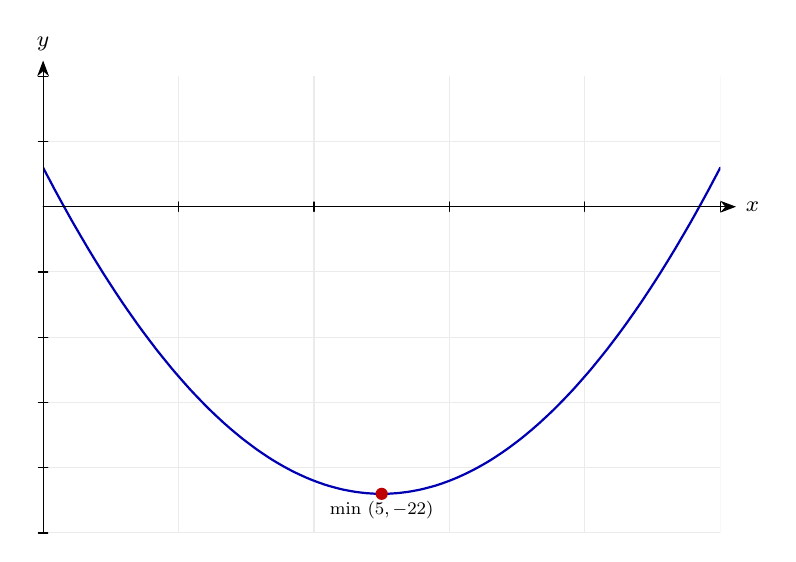
\begin{tikzpicture}[>={Stealth[length=2mm]},font=\footnotesize,line cap=round,line join=round]
\begin{scope}
\clip (0,0) rectangle (8.6,5.8);
\draw[gray!16] (0,0) grid[xstep=1.72,ystep=0.829] (8.6,5.8);
\draw[blue!70!black,thick] (0,4.64) -- (0.048,4.548) -- (0.096,4.458) -- (0.143,4.368) -- (0.191,4.28) -- (0.239,4.192) -- (0.287,4.106) -- (0.334,4.021) -- (0.382,3.936) -- (0.43,3.853) -- (0.478,3.771) -- (0.526,3.689) -- (0.573,3.609) -- (0.621,3.53) -- (0.669,3.451) -- (0.717,3.374) -- (0.764,3.298) -- (0.812,3.223) -- (0.86,3.149) -- (0.908,3.075) -- (0.956,3.003) -- (1.003,2.932) -- (1.051,2.862) -- (1.099,2.793) -- (1.147,2.725) -- (1.194,2.658) -- (1.242,2.592) -- (1.29,2.527) -- (1.338,2.463) -- (1.386,2.4) -- (1.433,2.338) -- (1.481,2.278) -- (1.529,2.218) -- (1.577,2.159) -- (1.624,2.101) -- (1.672,2.044) -- (1.72,1.989) -- (1.768,1.934) -- (1.816,1.88) -- (1.863,1.827) -- (1.911,1.776) -- (1.959,1.725) -- (2.007,1.676) -- (2.054,1.627) -- (2.102,1.579) -- (2.15,1.533) -- (2.198,1.487) -- (2.246,1.443) -- (2.293,1.399) -- (2.341,1.357) -- (2.389,1.315) -- (2.437,1.275) -- (2.484,1.236) -- (2.532,1.197) -- (2.58,1.16) -- (2.628,1.124) -- (2.676,1.088) -- (2.723,1.054) -- (2.771,1.021) -- (2.819,0.989) -- (2.867,0.957) -- (2.914,0.927) -- (2.962,0.898) -- (3.01,0.87) -- (3.058,0.843) -- (3.106,0.817) -- (3.153,0.792) -- (3.201,0.768) -- (3.249,0.745) -- (3.297,0.723) -- (3.344,0.702) -- (3.392,0.682) -- (3.44,0.663) -- (3.488,0.645) -- (3.536,0.628) -- (3.583,0.612) -- (3.631,0.597) -- (3.679,0.584) -- (3.727,0.571) -- (3.774,0.559) -- (3.822,0.548) -- (3.87,0.539) -- (3.918,0.53) -- (3.966,0.522) -- (4.013,0.516) -- (4.061,0.51) -- (4.109,0.505) -- (4.157,0.502) -- (4.204,0.499) -- (4.252,0.498) -- (4.3,0.497) -- (4.348,0.498) -- (4.396,0.499) -- (4.443,0.502) -- (4.491,0.505) -- (4.539,0.51) -- (4.587,0.516) -- (4.634,0.522) -- (4.682,0.53) -- (4.73,0.539) -- (4.778,0.548) -- (4.826,0.559) -- (4.873,0.571) -- (4.921,0.584) -- (4.969,0.597) -- (5.017,0.612) -- (5.064,0.628) -- (5.112,0.645) -- (5.16,0.663) -- (5.208,0.682) -- (5.256,0.702) -- (5.303,0.723) -- (5.351,0.745) -- (5.399,0.768) -- (5.447,0.792) -- (5.494,0.817) -- (5.542,0.843) -- (5.59,0.87) -- (5.638,0.898) -- (5.686,0.927) -- (5.733,0.957) -- (5.781,0.989) -- (5.829,1.021) -- (5.877,1.054) -- (5.924,1.088) -- (5.972,1.124) -- (6.02,1.16) -- (6.068,1.197) -- (6.116,1.236) -- (6.163,1.275) -- (6.211,1.315) -- (6.259,1.357) -- (6.307,1.399) -- (6.354,1.443) -- (6.402,1.487) -- (6.45,1.533) -- (6.498,1.579) -- (6.546,1.627) -- (6.593,1.676) -- (6.641,1.725) -- (6.689,1.776) -- (6.737,1.827) -- (6.784,1.88) -- (6.832,1.934) -- (6.88,1.989) -- (6.928,2.044) -- (6.976,2.101) -- (7.023,2.159) -- (7.071,2.218) -- (7.119,2.278) -- (7.167,2.338) -- (7.214,2.4) -- (7.262,2.463) -- (7.31,2.527) -- (7.358,2.592) -- (7.406,2.658) -- (7.453,2.725) -- (7.501,2.793) -- (7.549,2.862) -- (7.597,2.932) -- (7.644,3.003) -- (7.692,3.075) -- (7.74,3.149) -- (7.788,3.223) -- (7.836,3.298) -- (7.883,3.374) -- (7.931,3.451) -- (7.979,3.53) -- (8.027,3.609) -- (8.074,3.689) -- (8.122,3.771) -- (8.17,3.853) -- (8.218,3.936) -- (8.266,4.021) -- (8.313,4.106) -- (8.361,4.192) -- (8.409,4.28) -- (8.457,4.368) -- (8.504,4.458) -- (8.552,4.548) -- (8.6,4.64);
\end{scope}
\draw[->] (0,4.143) -- (8.8,4.143) node[right]{$x$};
\draw[->] (0,0) -- (0,6) node[above]{$y$};
\draw (1.72,4.083) -- (1.72,4.203);
\draw (3.44,4.083) -- (3.44,4.203);
\draw (5.16,4.083) -- (5.16,4.203);
\draw (6.88,4.083) -- (6.88,4.203);
\draw (8.6,4.083) -- (8.6,4.203);
\draw (-0.06,0) -- (0.06,0);
\draw (-0.06,0.829) -- (0.06,0.829);
\draw (-0.06,1.657) -- (0.06,1.657);
\draw (-0.06,2.486) -- (0.06,2.486);
\draw (-0.06,3.314) -- (0.06,3.314);
\draw (-0.06,4.971) -- (0.06,4.971);
\draw (-0.06,5.8) -- (0.06,5.8);
\fill[red!75!black] (4.3,0.497) circle (2.2pt);
\node[below,scale=0.8] at (4.3,0.497) {min $(5,-22)$};
\end{tikzpicture}
}
\end{center}
\small Curve with classified stationary points marked.\normalsize

\medskip\hrule

\section*{Derivatives and Graphs 02\quad\small\texttt{(d4-002)}}
\addcontentsline{toc}{section}{Derivatives and Graphs 02 (d4-002)}
\textit{Difficulty: Foundation \quad\textbar\quad Marks: 3}

\question{Find the \( x \)-coordinates of the stationary points of \( y = x^3 - 3x^2 - 24x + 1 \).}

\textbf{Worked solution.}

\textit{Step 1: Differentiate.}
\[\begin{gathered}
\frac{\mathrm{d}y}{\mathrm{d}x} = 3x^2 - 6x - 24
\end{gathered}\]
Apply the power rule.

\textit{Step 2: Set equal to zero.}
\[\begin{gathered}
3x^2 - 6x - 24 = 0 \implies x^2 - 2x - 8 = 0
\end{gathered}\]
Divide through by 3.

\textit{Step 3: Factorise and solve.}
\[\begin{gathered}
(x - 4)(x + 2) = 0 \implies x = 4 \text{ or } x = -2
\end{gathered}\]
Two numbers that multiply to \(-8\) and add to \(-2\) are \(-4\) and \(+2\).

\begin{answerbox}
\textbf{Final answer:}\quad \(\displaystyle  x = 4 \) and \(\displaystyle  x = -2 \)
\end{answerbox}
\textbf{Diagram.}

\begin{center}
\resizebox{\ifdim\width>\linewidth \linewidth\else \width\fi}{!}{%
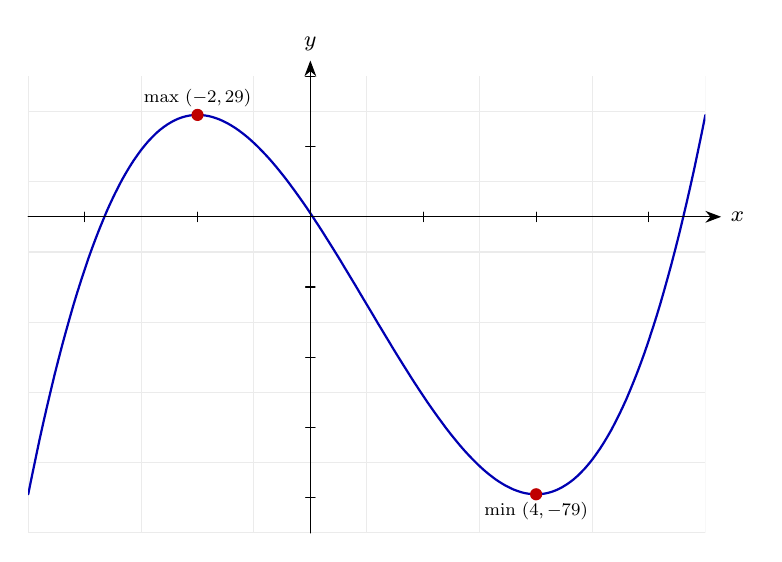
\begin{tikzpicture}[>={Stealth[length=2mm]},font=\footnotesize,line cap=round,line join=round]
\begin{scope}
\clip (0,0) rectangle (8.6,5.8);
\draw[gray!16] (-0.717,-0.446) grid[xstep=1.433,ystep=0.892] (8.6,5.8);
\draw[blue!70!black,thick] (0,0.491) -- (0.048,0.728) -- (0.096,0.958) -- (0.143,1.182) -- (0.191,1.398) -- (0.239,1.608) -- (0.287,1.811) -- (0.334,2.007) -- (0.382,2.196) -- (0.43,2.38) -- (0.478,2.556) -- (0.526,2.727) -- (0.573,2.891) -- (0.621,3.049) -- (0.669,3.2) -- (0.717,3.346) -- (0.764,3.486) -- (0.812,3.62) -- (0.86,3.748) -- (0.908,3.87) -- (0.956,3.987) -- (1.003,4.099) -- (1.051,4.204) -- (1.099,4.305) -- (1.147,4.4) -- (1.194,4.49) -- (1.242,4.574) -- (1.29,4.654) -- (1.338,4.729) -- (1.386,4.798) -- (1.433,4.863) -- (1.481,4.923) -- (1.529,4.979) -- (1.577,5.029) -- (1.624,5.076) -- (1.672,5.118) -- (1.72,5.155) -- (1.768,5.188) -- (1.816,5.217) -- (1.863,5.242) -- (1.911,5.263) -- (1.959,5.28) -- (2.007,5.293) -- (2.054,5.302) -- (2.102,5.307) -- (2.15,5.309) -- (2.198,5.307) -- (2.246,5.302) -- (2.293,5.294) -- (2.341,5.282) -- (2.389,5.266) -- (2.437,5.248) -- (2.484,5.226) -- (2.532,5.202) -- (2.58,5.174) -- (2.628,5.144) -- (2.676,5.111) -- (2.723,5.075) -- (2.771,5.037) -- (2.819,4.996) -- (2.867,4.952) -- (2.914,4.907) -- (2.962,4.858) -- (3.01,4.808) -- (3.058,4.756) -- (3.106,4.701) -- (3.153,4.645) -- (3.201,4.586) -- (3.249,4.526) -- (3.297,4.464) -- (3.344,4.4) -- (3.392,4.335) -- (3.44,4.268) -- (3.488,4.2) -- (3.536,4.131) -- (3.583,4.06) -- (3.631,3.988) -- (3.679,3.915) -- (3.727,3.841) -- (3.774,3.766) -- (3.822,3.69) -- (3.87,3.613) -- (3.918,3.536) -- (3.966,3.458) -- (4.013,3.379) -- (4.061,3.3) -- (4.109,3.22) -- (4.157,3.141) -- (4.204,3.061) -- (4.252,2.98) -- (4.3,2.9) -- (4.348,2.82) -- (4.396,2.739) -- (4.443,2.659) -- (4.491,2.58) -- (4.539,2.5) -- (4.587,2.421) -- (4.634,2.342) -- (4.682,2.264) -- (4.73,2.187) -- (4.778,2.11) -- (4.826,2.034) -- (4.873,1.959) -- (4.921,1.885) -- (4.969,1.812) -- (5.017,1.74) -- (5.064,1.669) -- (5.112,1.6) -- (5.16,1.532) -- (5.208,1.465) -- (5.256,1.4) -- (5.303,1.336) -- (5.351,1.274) -- (5.399,1.214) -- (5.447,1.155) -- (5.494,1.099) -- (5.542,1.044) -- (5.59,0.992) -- (5.638,0.942) -- (5.686,0.893) -- (5.733,0.848) -- (5.781,0.804) -- (5.829,0.763) -- (5.877,0.725) -- (5.924,0.689) -- (5.972,0.656) -- (6.02,0.626) -- (6.068,0.598) -- (6.116,0.574) -- (6.163,0.552) -- (6.211,0.534) -- (6.259,0.518) -- (6.307,0.506) -- (6.354,0.498) -- (6.402,0.493) -- (6.45,0.491) -- (6.498,0.493) -- (6.546,0.498) -- (6.593,0.507) -- (6.641,0.52) -- (6.689,0.537) -- (6.737,0.558) -- (6.784,0.583) -- (6.832,0.612) -- (6.88,0.645) -- (6.928,0.682) -- (6.976,0.724) -- (7.023,0.771) -- (7.071,0.821) -- (7.119,0.877) -- (7.167,0.937) -- (7.214,1.002) -- (7.262,1.071) -- (7.31,1.146) -- (7.358,1.226) -- (7.406,1.31) -- (7.453,1.4) -- (7.501,1.495) -- (7.549,1.596) -- (7.597,1.701) -- (7.644,1.813) -- (7.692,1.93) -- (7.74,2.052) -- (7.788,2.18) -- (7.836,2.314) -- (7.883,2.454) -- (7.931,2.6) -- (7.979,2.751) -- (8.027,2.909) -- (8.074,3.073) -- (8.122,3.244) -- (8.17,3.42) -- (8.218,3.604) -- (8.266,3.793) -- (8.313,3.989) -- (8.361,4.192) -- (8.409,4.402) -- (8.457,4.618) -- (8.504,4.842) -- (8.552,5.072) -- (8.6,5.309);
\end{scope}
\draw[->] (0,4.015) -- (8.8,4.015) node[right]{$x$};
\draw[->] (3.583,0) -- (3.583,6) node[above]{$y$};
\draw (0.717,3.955) -- (0.717,4.075);
\draw (2.15,3.955) -- (2.15,4.075);
\draw (5.017,3.955) -- (5.017,4.075);
\draw (6.45,3.955) -- (6.45,4.075);
\draw (7.883,3.955) -- (7.883,4.075);
\draw (3.523,0.446) -- (3.643,0.446);
\draw (3.523,1.338) -- (3.643,1.338);
\draw (3.523,2.231) -- (3.643,2.231);
\draw (3.523,3.123) -- (3.643,3.123);
\draw (3.523,4.908) -- (3.643,4.908);
\draw (3.523,5.8) -- (3.643,5.8);
\fill[red!75!black] (2.15,5.309) circle (2.2pt);
\node[above,scale=0.8] at (2.15,5.309) {max $(-2,29)$};
\fill[red!75!black] (6.45,0.491) circle (2.2pt);
\node[below,scale=0.8] at (6.45,0.491) {min $(4,-79)$};
\end{tikzpicture}
}
\end{center}
\small Curve with classified stationary points marked.\normalsize

\medskip\hrule

\section*{Derivatives and Graphs 03\quad\small\texttt{(d4-003)}}
\addcontentsline{toc}{section}{Derivatives and Graphs 03 (d4-003)}
\textit{Difficulty: Foundation \quad\textbar\quad Marks: 4}

\question{Find the coordinates of the stationary points of \( y = 2x^3 - 9x^2 + 12x - 3 \).}

\textbf{Worked solution.}

\textit{Step 1: Differentiate.}
\[\begin{gathered}
\frac{\mathrm{d}y}{\mathrm{d}x} = 6x^2 - 18x + 12
\end{gathered}\]
Power rule.

\textit{Step 2: Solve \( \dfrac{\mathrm{d}y}{\mathrm{d}x} = 0 \).}
\[\begin{gathered}
6x^2 - 18x + 12 = 0 \implies x^2 - 3x + 2 = 0 \implies (x-1)(x-2) = 0
\end{gathered}\]
Divide by 6, then factorise.

\textit{Step 3: Find \( y \)-coordinates.}
\[\begin{gathered}
x=1: y = 2 - 9 + 12 - 3 = 2 \newline x=2: y = 16 - 36 + 24 - 3 = 1
\end{gathered}\]
Substitute each \( x \) back into the original equation.

\begin{answerbox}
\textbf{Final answer:}\quad \(\displaystyle  (1, 2) \) and \(\displaystyle  (2, 1) \)
\end{answerbox}
\textbf{Diagram.}

\begin{center}
\resizebox{\ifdim\width>\linewidth \linewidth\else \width\fi}{!}{%
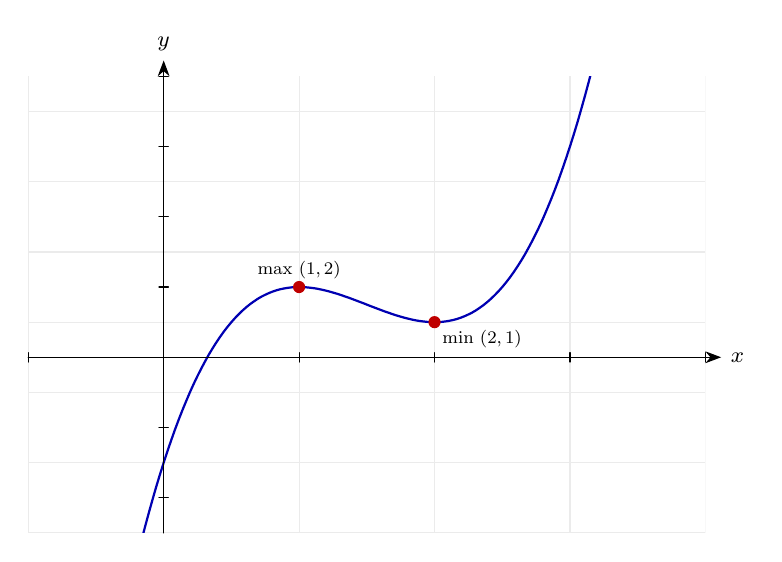
\begin{tikzpicture}[>={Stealth[length=2mm]},font=\footnotesize,line cap=round,line join=round]
\begin{scope}
\clip (0,0) rectangle (8.6,5.8);
\draw[gray!16] (0,-0.446) grid[xstep=1.72,ystep=0.892] (8.6,5.8);
\draw[blue!70!black,thick] (0,-5.8) -- (0.048,-5.8) -- (0.096,-5.8) -- (0.143,-5.8) -- (0.191,-5.8) -- (0.239,-5.8) -- (0.287,-5.8) -- (0.334,-5.8) -- (0.382,-5.8) -- (0.43,-5.758) -- (0.478,-5.405) -- (0.526,-5.061) -- (0.573,-4.726) -- (0.621,-4.4) -- (0.669,-4.083) -- (0.717,-3.774) -- (0.764,-3.474) -- (0.812,-3.183) -- (0.86,-2.9) -- (0.908,-2.625) -- (0.956,-2.359) -- (1.003,-2.1) -- (1.051,-1.849) -- (1.099,-1.607) -- (1.147,-1.372) -- (1.194,-1.144) -- (1.242,-0.924) -- (1.29,-0.711) -- (1.338,-0.506) -- (1.386,-0.307) -- (1.433,-0.116) -- (1.481,0.069) -- (1.529,0.247) -- (1.577,0.418) -- (1.624,0.582) -- (1.672,0.74) -- (1.72,0.892) -- (1.768,1.038) -- (1.816,1.178) -- (1.863,1.311) -- (1.911,1.439) -- (1.959,1.561) -- (2.007,1.677) -- (2.054,1.788) -- (2.102,1.894) -- (2.15,1.994) -- (2.198,2.089) -- (2.246,2.179) -- (2.293,2.264) -- (2.341,2.344) -- (2.389,2.42) -- (2.437,2.491) -- (2.484,2.557) -- (2.532,2.619) -- (2.58,2.677) -- (2.628,2.731) -- (2.676,2.78) -- (2.723,2.826) -- (2.771,2.868) -- (2.819,2.907) -- (2.867,2.941) -- (2.914,2.973) -- (2.962,3.001) -- (3.01,3.025) -- (3.058,3.047) -- (3.106,3.066) -- (3.153,3.082) -- (3.201,3.095) -- (3.249,3.105) -- (3.297,3.113) -- (3.344,3.119) -- (3.392,3.122) -- (3.44,3.123) -- (3.488,3.122) -- (3.536,3.119) -- (3.583,3.114) -- (3.631,3.108) -- (3.679,3.1) -- (3.727,3.09) -- (3.774,3.079) -- (3.822,3.067) -- (3.87,3.053) -- (3.918,3.039) -- (3.966,3.024) -- (4.013,3.007) -- (4.061,2.991) -- (4.109,2.973) -- (4.157,2.955) -- (4.204,2.937) -- (4.252,2.919) -- (4.3,2.9) -- (4.348,2.881) -- (4.396,2.863) -- (4.443,2.845) -- (4.491,2.827) -- (4.539,2.809) -- (4.587,2.793) -- (4.634,2.776) -- (4.682,2.761) -- (4.73,2.747) -- (4.778,2.733) -- (4.826,2.721) -- (4.873,2.71) -- (4.921,2.7) -- (4.969,2.692) -- (5.017,2.686) -- (5.064,2.681) -- (5.112,2.678) -- (5.16,2.677) -- (5.208,2.678) -- (5.256,2.681) -- (5.303,2.687) -- (5.351,2.695) -- (5.399,2.705) -- (5.447,2.718) -- (5.494,2.734) -- (5.542,2.753) -- (5.59,2.775) -- (5.638,2.799) -- (5.686,2.827) -- (5.733,2.859) -- (5.781,2.893) -- (5.829,2.932) -- (5.877,2.974) -- (5.924,3.02) -- (5.972,3.069) -- (6.02,3.123) -- (6.068,3.181) -- (6.116,3.243) -- (6.163,3.309) -- (6.211,3.38) -- (6.259,3.456) -- (6.307,3.536) -- (6.354,3.621) -- (6.402,3.711) -- (6.45,3.806) -- (6.498,3.906) -- (6.546,4.012) -- (6.593,4.123) -- (6.641,4.239) -- (6.689,4.361) -- (6.737,4.489) -- (6.784,4.622) -- (6.832,4.762) -- (6.88,4.908) -- (6.928,5.06) -- (6.976,5.218) -- (7.023,5.382) -- (7.071,5.553) -- (7.119,5.731) -- (7.167,5.916) -- (7.214,6.107) -- (7.262,6.306) -- (7.31,6.511) -- (7.358,6.724) -- (7.406,6.944) -- (7.453,7.172) -- (7.501,7.407) -- (7.549,7.649) -- (7.597,7.9) -- (7.644,8.159) -- (7.692,8.425) -- (7.74,8.7) -- (7.788,8.983) -- (7.836,9.274) -- (7.883,9.574) -- (7.931,9.883) -- (7.979,10.2) -- (8.027,10.526) -- (8.074,10.861) -- (8.122,11.205) -- (8.17,11.558) -- (8.218,11.6) -- (8.266,11.6) -- (8.313,11.6) -- (8.361,11.6) -- (8.409,11.6) -- (8.457,11.6) -- (8.504,11.6) -- (8.552,11.6) -- (8.6,11.6);
\end{scope}
\draw[->] (0,2.231) -- (8.8,2.231) node[right]{$x$};
\draw[->] (1.72,0) -- (1.72,6) node[above]{$y$};
\draw (0,2.171) -- (0,2.291);
\draw (3.44,2.171) -- (3.44,2.291);
\draw (5.16,2.171) -- (5.16,2.291);
\draw (6.88,2.171) -- (6.88,2.291);
\draw (8.6,2.171) -- (8.6,2.291);
\draw (1.66,0.446) -- (1.78,0.446);
\draw (1.66,1.338) -- (1.78,1.338);
\draw (1.66,3.123) -- (1.78,3.123);
\draw (1.66,4.015) -- (1.78,4.015);
\draw (1.66,4.908) -- (1.78,4.908);
\draw (1.66,5.8) -- (1.78,5.8);
\fill[red!75!black] (3.44,3.123) circle (2.2pt);
\node[above,scale=0.8] at (3.44,3.123) {max $(1,2)$};
\fill[red!75!black] (5.16,2.677) circle (2.2pt);
\node[below right,scale=0.8] at (5.16,2.677) {min $(2,1)$};
\end{tikzpicture}
}
\end{center}
\small Curve with classified stationary points marked.\normalsize

\medskip\hrule

\section*{Derivatives and Graphs 04\quad\small\texttt{(d4-004)}}
\addcontentsline{toc}{section}{Derivatives and Graphs 04 (d4-004)}
\textit{Difficulty: Foundation \quad\textbar\quad Marks: 4}

\question{Find the coordinates of the stationary point of \( y = -x^2 + 8x - 10 \) and state its nature.}

\textbf{Worked solution.}

\textit{Step 1: Differentiate.}
\[\begin{gathered}
\frac{\mathrm{d}y}{\mathrm{d}x} = -2x + 8
\end{gathered}\]
Power rule.

\textit{Step 2: Set to zero and solve.}
\[\begin{gathered}
-2x + 8 = 0 \implies x = 4
\end{gathered}\]
Solve the linear equation.

\textit{Step 3: Find \( y \).}
\[\begin{gathered}
y = -16 + 32 - 10 = 6
\end{gathered}\]
Substitute \( x = 4 \).

\textit{Step 4: Determine nature using second derivative.}
\[\begin{gathered}
\frac{\mathrm{d}^2y}{\mathrm{d}x^2} = -2 < 0 \Rightarrow \text{maximum}
\end{gathered}\]
The second derivative is constant and negative, so this is a maximum.

\begin{answerbox}
\textbf{Final answer:}\quad Local maximum at \(\displaystyle  (4, 6) \)
\end{answerbox}
\textbf{Diagram.}

\begin{center}
\resizebox{\ifdim\width>\linewidth \linewidth\else \width\fi}{!}{%
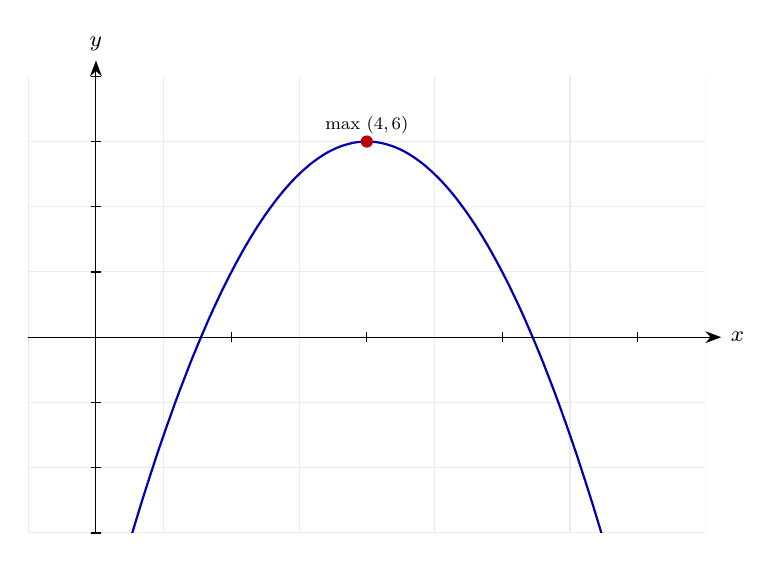
\begin{tikzpicture}[>={Stealth[length=2mm]},font=\footnotesize,line cap=round,line join=round]
\begin{scope}
\clip (0,0) rectangle (8.6,5.8);
\draw[gray!16] (-0.86,0) grid[xstep=1.72,ystep=0.829] (8.6,5.8);
\draw[blue!70!black,thick] (0,-5.386) -- (0.048,-5.157) -- (0.096,-4.931) -- (0.143,-4.707) -- (0.191,-4.486) -- (0.239,-4.267) -- (0.287,-4.051) -- (0.334,-3.837) -- (0.382,-3.626) -- (0.43,-3.418) -- (0.478,-3.212) -- (0.526,-3.009) -- (0.573,-2.808) -- (0.621,-2.61) -- (0.669,-2.414) -- (0.717,-2.221) -- (0.764,-2.031) -- (0.812,-1.843) -- (0.86,-1.657) -- (0.908,-1.474) -- (0.956,-1.294) -- (1.003,-1.116) -- (1.051,-0.941) -- (1.099,-0.768) -- (1.147,-0.598) -- (1.194,-0.431) -- (1.242,-0.266) -- (1.29,-0.104) -- (1.338,0.056) -- (1.386,0.214) -- (1.433,0.368) -- (1.481,0.52) -- (1.529,0.67) -- (1.577,0.817) -- (1.624,0.962) -- (1.672,1.103) -- (1.72,1.243) -- (1.768,1.38) -- (1.816,1.514) -- (1.863,1.646) -- (1.911,1.775) -- (1.959,1.901) -- (2.007,2.025) -- (2.054,2.147) -- (2.102,2.266) -- (2.15,2.382) -- (2.198,2.496) -- (2.246,2.607) -- (2.293,2.716) -- (2.341,2.822) -- (2.389,2.926) -- (2.437,3.027) -- (2.484,3.125) -- (2.532,3.221) -- (2.58,3.314) -- (2.628,3.405) -- (2.676,3.493) -- (2.723,3.579) -- (2.771,3.662) -- (2.819,3.743) -- (2.867,3.821) -- (2.914,3.896) -- (2.962,3.969) -- (3.01,4.039) -- (3.058,4.107) -- (3.106,4.172) -- (3.153,4.235) -- (3.201,4.295) -- (3.249,4.353) -- (3.297,4.408) -- (3.344,4.46) -- (3.392,4.51) -- (3.44,4.557) -- (3.488,4.602) -- (3.536,4.644) -- (3.583,4.684) -- (3.631,4.721) -- (3.679,4.755) -- (3.727,4.787) -- (3.774,4.817) -- (3.822,4.844) -- (3.87,4.868) -- (3.918,4.89) -- (3.966,4.909) -- (4.013,4.925) -- (4.061,4.939) -- (4.109,4.951) -- (4.157,4.96) -- (4.204,4.966) -- (4.252,4.97) -- (4.3,4.971) -- (4.348,4.97) -- (4.396,4.966) -- (4.443,4.96) -- (4.491,4.951) -- (4.539,4.939) -- (4.587,4.925) -- (4.634,4.909) -- (4.682,4.89) -- (4.73,4.868) -- (4.778,4.844) -- (4.826,4.817) -- (4.873,4.787) -- (4.921,4.755) -- (4.969,4.721) -- (5.017,4.684) -- (5.064,4.644) -- (5.112,4.602) -- (5.16,4.557) -- (5.208,4.51) -- (5.256,4.46) -- (5.303,4.408) -- (5.351,4.353) -- (5.399,4.295) -- (5.447,4.235) -- (5.494,4.172) -- (5.542,4.107) -- (5.59,4.039) -- (5.638,3.969) -- (5.686,3.896) -- (5.733,3.821) -- (5.781,3.743) -- (5.829,3.662) -- (5.877,3.579) -- (5.924,3.493) -- (5.972,3.405) -- (6.02,3.314) -- (6.068,3.221) -- (6.116,3.125) -- (6.163,3.027) -- (6.211,2.926) -- (6.259,2.822) -- (6.307,2.716) -- (6.354,2.607) -- (6.402,2.496) -- (6.45,2.382) -- (6.498,2.266) -- (6.546,2.147) -- (6.593,2.025) -- (6.641,1.901) -- (6.689,1.775) -- (6.737,1.646) -- (6.784,1.514) -- (6.832,1.38) -- (6.88,1.243) -- (6.928,1.103) -- (6.976,0.962) -- (7.023,0.817) -- (7.071,0.67) -- (7.119,0.52) -- (7.167,0.368) -- (7.214,0.214) -- (7.262,0.056) -- (7.31,-0.104) -- (7.358,-0.266) -- (7.406,-0.431) -- (7.453,-0.598) -- (7.501,-0.768) -- (7.549,-0.941) -- (7.597,-1.116) -- (7.644,-1.294) -- (7.692,-1.474) -- (7.74,-1.657) -- (7.788,-1.843) -- (7.836,-2.031) -- (7.883,-2.221) -- (7.931,-2.414) -- (7.979,-2.61) -- (8.027,-2.808) -- (8.074,-3.009) -- (8.122,-3.212) -- (8.17,-3.418) -- (8.218,-3.626) -- (8.266,-3.837) -- (8.313,-4.051) -- (8.361,-4.267) -- (8.409,-4.486) -- (8.457,-4.707) -- (8.504,-4.931) -- (8.552,-5.157) -- (8.6,-5.386);
\end{scope}
\draw[->] (0,2.486) -- (8.8,2.486) node[right]{$x$};
\draw[->] (0.86,0) -- (0.86,6) node[above]{$y$};
\draw (2.58,2.426) -- (2.58,2.546);
\draw (4.3,2.426) -- (4.3,2.546);
\draw (6.02,2.426) -- (6.02,2.546);
\draw (7.74,2.426) -- (7.74,2.546);
\draw (0.8,0) -- (0.92,0);
\draw (0.8,0.829) -- (0.92,0.829);
\draw (0.8,1.657) -- (0.92,1.657);
\draw (0.8,3.314) -- (0.92,3.314);
\draw (0.8,4.143) -- (0.92,4.143);
\draw (0.8,4.971) -- (0.92,4.971);
\draw (0.8,5.8) -- (0.92,5.8);
\fill[red!75!black] (4.3,4.971) circle (2.2pt);
\node[above,scale=0.8] at (4.3,4.971) {max $(4,6)$};
\end{tikzpicture}
}
\end{center}
\small Curve with classified stationary points marked.\normalsize

\medskip\hrule

\section*{Derivatives and Graphs 05\quad\small\texttt{(d4-005)}}
\addcontentsline{toc}{section}{Derivatives and Graphs 05 (d4-005)}
\textit{Difficulty: Foundation \quad\textbar\quad Marks: 6}

\question{Find the coordinates of the stationary points of \( y = x^3 + 3x^2 - 45x + 7 \) and classify each one.}

\textbf{Worked solution.}

\textit{Step 1: Differentiate.}
\[\begin{gathered}
\frac{\mathrm{d}y}{\mathrm{d}x} = 3x^2 + 6x - 45
\end{gathered}\]
Power rule.

\textit{Step 2: Solve \( \dfrac{\mathrm{d}y}{\mathrm{d}x} = 0 \).}
\[\begin{gathered}
x^2 + 2x - 15 = 0 \implies (x + 5)(x - 3) = 0 \implies x = -5 \text{ or } x = 3
\end{gathered}\]
Divide by 3 then factorise.

\textit{Step 3: Find \( y \)-coordinates.}
\[\begin{gathered}
x=-5: y = -125 + 75 + 225 + 7 = 182 \newline x=3: y = 27 + 27 - 135 + 7 = -74
\end{gathered}\]
Substitute into the original equation.

\textit{Step 4: Second derivative.}
\[\begin{gathered}
\frac{\mathrm{d}^2y}{\mathrm{d}x^2} = 6x + 6
\end{gathered}\]
Differentiate the first derivative.

\textit{Step 5: Classify each point.}
\[\begin{gathered}
x=-5: 6(-5)+6 = -24 < 0 \Rightarrow \text{maximum} \newline x=3: 6(3)+6 = 24 > 0 \Rightarrow \text{minimum}
\end{gathered}\]
Substitute into \( \dfrac{\mathrm{d}^2y}{\mathrm{d}x^2} \).

\begin{answerbox}
\textbf{Final answer:}\quad Local maximum at \(\displaystyle  (-5, 182) \); local minimum at \(\displaystyle  (3, -74) \)
\end{answerbox}
\textbf{Diagram.}

\begin{center}
\resizebox{\ifdim\width>\linewidth \linewidth\else \width\fi}{!}{%
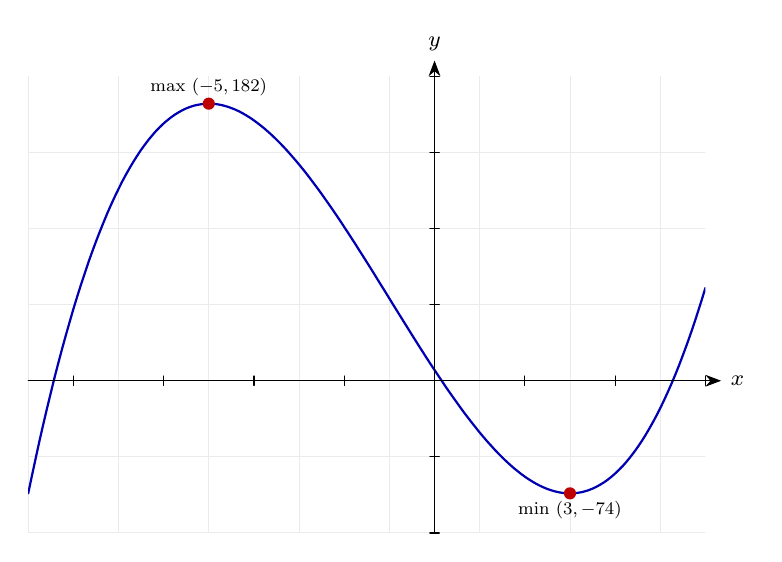
\begin{tikzpicture}[>={Stealth[length=2mm]},font=\footnotesize,line cap=round,line join=round]
\begin{scope}
\clip (0,0) rectangle (8.6,5.8);
\draw[gray!16] (-0.573,0) grid[xstep=1.147,ystep=0.967] (8.6,5.8);
\draw[blue!70!black,thick] (0,0.503) -- (0.048,0.731) -- (0.096,0.954) -- (0.143,1.17) -- (0.191,1.38) -- (0.239,1.584) -- (0.287,1.781) -- (0.334,1.973) -- (0.382,2.158) -- (0.43,2.338) -- (0.478,2.512) -- (0.526,2.68) -- (0.573,2.842) -- (0.621,2.999) -- (0.669,3.15) -- (0.717,3.295) -- (0.764,3.436) -- (0.812,3.57) -- (0.86,3.7) -- (0.908,3.824) -- (0.956,3.943) -- (1.003,4.057) -- (1.051,4.166) -- (1.099,4.27) -- (1.147,4.369) -- (1.194,4.464) -- (1.242,4.553) -- (1.29,4.638) -- (1.338,4.718) -- (1.386,4.794) -- (1.433,4.865) -- (1.481,4.931) -- (1.529,4.994) -- (1.577,5.052) -- (1.624,5.106) -- (1.672,5.155) -- (1.72,5.201) -- (1.768,5.242) -- (1.816,5.28) -- (1.863,5.313) -- (1.911,5.343) -- (1.959,5.369) -- (2.007,5.392) -- (2.054,5.41) -- (2.102,5.426) -- (2.15,5.437) -- (2.198,5.445) -- (2.246,5.45) -- (2.293,5.452) -- (2.341,5.45) -- (2.389,5.446) -- (2.437,5.438) -- (2.484,5.427) -- (2.532,5.413) -- (2.58,5.396) -- (2.628,5.377) -- (2.676,5.355) -- (2.723,5.33) -- (2.771,5.302) -- (2.819,5.272) -- (2.867,5.239) -- (2.914,5.204) -- (2.962,5.167) -- (3.01,5.127) -- (3.058,5.085) -- (3.106,5.041) -- (3.153,4.995) -- (3.201,4.947) -- (3.249,4.897) -- (3.297,4.845) -- (3.344,4.791) -- (3.392,4.736) -- (3.44,4.679) -- (3.488,4.62) -- (3.536,4.56) -- (3.583,4.498) -- (3.631,4.434) -- (3.679,4.37) -- (3.727,4.304) -- (3.774,4.237) -- (3.822,4.169) -- (3.87,4.1) -- (3.918,4.029) -- (3.966,3.958) -- (4.013,3.886) -- (4.061,3.813) -- (4.109,3.739) -- (4.157,3.665) -- (4.204,3.59) -- (4.252,3.515) -- (4.3,3.439) -- (4.348,3.363) -- (4.396,3.286) -- (4.443,3.209) -- (4.491,3.132) -- (4.539,3.055) -- (4.587,2.977) -- (4.634,2.9) -- (4.682,2.823) -- (4.73,2.746) -- (4.778,2.669) -- (4.826,2.592) -- (4.873,2.516) -- (4.921,2.44) -- (4.969,2.364) -- (5.017,2.289) -- (5.064,2.215) -- (5.112,2.142) -- (5.16,2.069) -- (5.208,1.997) -- (5.256,1.925) -- (5.303,1.855) -- (5.351,1.786) -- (5.399,1.718) -- (5.447,1.651) -- (5.494,1.585) -- (5.542,1.52) -- (5.59,1.457) -- (5.638,1.395) -- (5.686,1.335) -- (5.733,1.276) -- (5.781,1.219) -- (5.829,1.163) -- (5.877,1.11) -- (5.924,1.058) -- (5.972,1.008) -- (6.02,0.959) -- (6.068,0.913) -- (6.116,0.869) -- (6.163,0.827) -- (6.211,0.788) -- (6.259,0.75) -- (6.307,0.715) -- (6.354,0.683) -- (6.402,0.653) -- (6.45,0.625) -- (6.498,0.6) -- (6.546,0.578) -- (6.593,0.558) -- (6.641,0.542) -- (6.689,0.528) -- (6.737,0.517) -- (6.784,0.509) -- (6.832,0.504) -- (6.88,0.503) -- (6.928,0.504) -- (6.976,0.509) -- (7.023,0.517) -- (7.071,0.529) -- (7.119,0.544) -- (7.167,0.563) -- (7.214,0.585) -- (7.262,0.612) -- (7.31,0.641) -- (7.358,0.675) -- (7.406,0.713) -- (7.453,0.754) -- (7.501,0.8) -- (7.549,0.849) -- (7.597,0.903) -- (7.644,0.961) -- (7.692,1.023) -- (7.74,1.09) -- (7.788,1.161) -- (7.836,1.237) -- (7.883,1.317) -- (7.931,1.402) -- (7.979,1.491) -- (8.027,1.585) -- (8.074,1.684) -- (8.122,1.788) -- (8.17,1.897) -- (8.218,2.011) -- (8.266,2.13) -- (8.313,2.255) -- (8.361,2.384) -- (8.409,2.519) -- (8.457,2.659) -- (8.504,2.805) -- (8.552,2.956) -- (8.6,3.113);
\end{scope}
\draw[->] (0,1.933) -- (8.8,1.933) node[right]{$x$};
\draw[->] (5.16,0) -- (5.16,6) node[above]{$y$};
\draw (0.573,1.873) -- (0.573,1.993);
\draw (1.72,1.873) -- (1.72,1.993);
\draw (2.867,1.873) -- (2.867,1.993);
\draw (4.013,1.873) -- (4.013,1.993);
\draw (6.307,1.873) -- (6.307,1.993);
\draw (7.453,1.873) -- (7.453,1.993);
\draw (8.6,1.873) -- (8.6,1.993);
\draw (5.1,0) -- (5.22,0);
\draw (5.1,0.967) -- (5.22,0.967);
\draw (5.1,2.9) -- (5.22,2.9);
\draw (5.1,3.867) -- (5.22,3.867);
\draw (5.1,4.833) -- (5.22,4.833);
\draw (5.1,5.8) -- (5.22,5.8);
\fill[red!75!black] (2.293,5.452) circle (2.2pt);
\node[above,scale=0.8] at (2.293,5.452) {max $(-5,182)$};
\fill[red!75!black] (6.88,0.503) circle (2.2pt);
\node[below,scale=0.8] at (6.88,0.503) {min $(3,-74)$};
\end{tikzpicture}
}
\end{center}
\small Curve with classified stationary points marked.\normalsize

\medskip\hrule

\section*{Derivatives and Graphs 06\quad\small\texttt{(d4-006)}}
\addcontentsline{toc}{section}{Derivatives and Graphs 06 (d4-006)}
\textit{Difficulty: Foundation \quad\textbar\quad Marks: 4}

\question{Show that the function \( f(x) = x^2 + 4x + 9 \) has no real roots, and find the coordinates of its stationary point.}

\textbf{Worked solution.}

\textit{Step 1: Check the discriminant for real roots.}
\[\begin{gathered}
\Delta = b^2 - 4ac = 16 - 36 = -20 < 0
\end{gathered}\]
Since \( \Delta < 0 \), the quadratic has no real roots --- it never crosses the \( x \)-axis.

\textit{Step 2: Find the stationary point.}
\[\begin{gathered}
f'(x) = 2x + 4 = 0 \implies x = -2
\end{gathered}\]
Set the derivative to zero.

\textit{Step 3: Find \( y \).}
\[\begin{gathered}
f(-2) = 4 - 8 + 9 = 5
\end{gathered}\]
Substitute \( x = -2 \).

\begin{answerbox}
\textbf{Final answer:}\quad No real roots (\(\displaystyle  \Delta = -20 < 0 \)); stationary point at \(\displaystyle  (-2, 5) \)
\end{answerbox}
\textbf{Diagram.}

\begin{center}
\resizebox{\ifdim\width>\linewidth \linewidth\else \width\fi}{!}{%
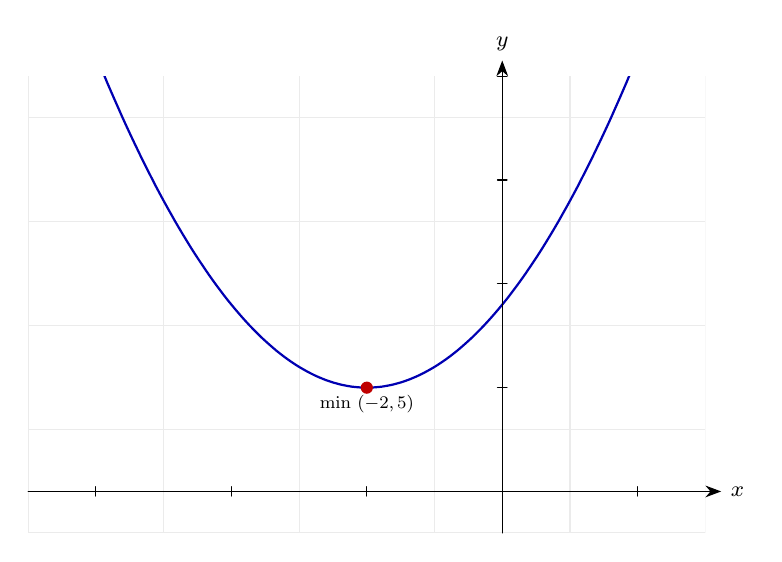
\begin{tikzpicture}[>={Stealth[length=2mm]},font=\footnotesize,line cap=round,line join=round]
\begin{scope}
\clip (0,0) rectangle (8.6,5.8);
\draw[gray!16] (-0.86,-0.791) grid[xstep=1.72,ystep=1.318] (8.6,5.8);
\draw[blue!70!black,thick] (0,8.436) -- (0.048,8.291) -- (0.096,8.147) -- (0.143,8.004) -- (0.191,7.864) -- (0.239,7.724) -- (0.287,7.587) -- (0.334,7.451) -- (0.382,7.317) -- (0.43,7.184) -- (0.478,7.053) -- (0.526,6.924) -- (0.573,6.796) -- (0.621,6.67) -- (0.669,6.545) -- (0.717,6.422) -- (0.764,6.301) -- (0.812,6.182) -- (0.86,6.064) -- (0.908,5.947) -- (0.956,5.833) -- (1.003,5.719) -- (1.051,5.608) -- (1.099,5.498) -- (1.147,5.39) -- (1.194,5.283) -- (1.242,5.178) -- (1.29,5.075) -- (1.338,4.973) -- (1.386,4.873) -- (1.433,4.775) -- (1.481,4.678) -- (1.529,4.583) -- (1.577,4.489) -- (1.624,4.397) -- (1.672,4.307) -- (1.72,4.218) -- (1.768,4.131) -- (1.816,4.046) -- (1.863,3.962) -- (1.911,3.88) -- (1.959,3.799) -- (2.007,3.72) -- (2.054,3.643) -- (2.102,3.567) -- (2.15,3.493) -- (2.198,3.421) -- (2.246,3.35) -- (2.293,3.281) -- (2.341,3.213) -- (2.389,3.147) -- (2.437,3.083) -- (2.484,3.02) -- (2.532,2.959) -- (2.58,2.9) -- (2.628,2.842) -- (2.676,2.786) -- (2.723,2.732) -- (2.771,2.679) -- (2.819,2.627) -- (2.867,2.578) -- (2.914,2.53) -- (2.962,2.483) -- (3.01,2.439) -- (3.058,2.396) -- (3.106,2.354) -- (3.153,2.314) -- (3.201,2.276) -- (3.249,2.239) -- (3.297,2.204) -- (3.344,2.171) -- (3.392,2.139) -- (3.44,2.109) -- (3.488,2.081) -- (3.536,2.054) -- (3.583,2.029) -- (3.631,2.005) -- (3.679,1.983) -- (3.727,1.963) -- (3.774,1.944) -- (3.822,1.927) -- (3.87,1.911) -- (3.918,1.898) -- (3.966,1.885) -- (4.013,1.875) -- (4.061,1.866) -- (4.109,1.858) -- (4.157,1.853) -- (4.204,1.849) -- (4.252,1.846) -- (4.3,1.845) -- (4.348,1.846) -- (4.396,1.849) -- (4.443,1.853) -- (4.491,1.858) -- (4.539,1.866) -- (4.587,1.875) -- (4.634,1.885) -- (4.682,1.898) -- (4.73,1.911) -- (4.778,1.927) -- (4.826,1.944) -- (4.873,1.963) -- (4.921,1.983) -- (4.969,2.005) -- (5.017,2.029) -- (5.064,2.054) -- (5.112,2.081) -- (5.16,2.109) -- (5.208,2.139) -- (5.256,2.171) -- (5.303,2.204) -- (5.351,2.239) -- (5.399,2.276) -- (5.447,2.314) -- (5.494,2.354) -- (5.542,2.396) -- (5.59,2.439) -- (5.638,2.483) -- (5.686,2.53) -- (5.733,2.578) -- (5.781,2.627) -- (5.829,2.679) -- (5.877,2.732) -- (5.924,2.786) -- (5.972,2.842) -- (6.02,2.9) -- (6.068,2.959) -- (6.116,3.02) -- (6.163,3.083) -- (6.211,3.147) -- (6.259,3.213) -- (6.307,3.281) -- (6.354,3.35) -- (6.402,3.421) -- (6.45,3.493) -- (6.498,3.567) -- (6.546,3.643) -- (6.593,3.72) -- (6.641,3.799) -- (6.689,3.88) -- (6.737,3.962) -- (6.784,4.046) -- (6.832,4.131) -- (6.88,4.218) -- (6.928,4.307) -- (6.976,4.397) -- (7.023,4.489) -- (7.071,4.583) -- (7.119,4.678) -- (7.167,4.775) -- (7.214,4.873) -- (7.262,4.973) -- (7.31,5.075) -- (7.358,5.178) -- (7.406,5.283) -- (7.453,5.39) -- (7.501,5.498) -- (7.549,5.608) -- (7.597,5.719) -- (7.644,5.833) -- (7.692,5.947) -- (7.74,6.064) -- (7.788,6.182) -- (7.836,6.301) -- (7.883,6.422) -- (7.931,6.545) -- (7.979,6.67) -- (8.027,6.796) -- (8.074,6.924) -- (8.122,7.053) -- (8.17,7.184) -- (8.218,7.317) -- (8.266,7.451) -- (8.313,7.587) -- (8.361,7.724) -- (8.409,7.864) -- (8.457,8.004) -- (8.504,8.147) -- (8.552,8.291) -- (8.6,8.436);
\end{scope}
\draw[->] (0,0.527) -- (8.8,0.527) node[right]{$x$};
\draw[->] (6.02,0) -- (6.02,6) node[above]{$y$};
\draw (0.86,0.467) -- (0.86,0.587);
\draw (2.58,0.467) -- (2.58,0.587);
\draw (4.3,0.467) -- (4.3,0.587);
\draw (7.74,0.467) -- (7.74,0.587);
\draw (5.96,1.845) -- (6.08,1.845);
\draw (5.96,3.164) -- (6.08,3.164);
\draw (5.96,4.482) -- (6.08,4.482);
\draw (5.96,5.8) -- (6.08,5.8);
\fill[red!75!black] (4.3,1.845) circle (2.2pt);
\node[below,scale=0.8] at (4.3,1.845) {min $(-2,5)$};
\end{tikzpicture}
}
\end{center}
\small Curve with classified stationary points marked.\normalsize

\medskip\hrule

\section*{Derivatives and Graphs 07\quad\small\texttt{(d4-007)}}
\addcontentsline{toc}{section}{Derivatives and Graphs 07 (d4-007)}
\textit{Difficulty: Foundation \quad\textbar\quad Marks: 3}

\question{Show that \( f(x) = x^3 + 5x + 2 \) has no stationary points.}

\textbf{Worked solution.}

\textit{Step 1: Differentiate.}
\[\begin{gathered}
f'(x) = 3x^2 + 5
\end{gathered}\]
Power rule.

\textit{Step 2: Set \( f'(x) = 0 \) and examine the equation.}
\[\begin{gathered}
3x^2 + 5 = 0 \implies x^2 = -\tfrac{5}{3}
\end{gathered}\]
This has no real solutions since \( x^2 \geq 0 \) for all real \( x \).

\textit{Step 3: Conclude.}
\[\begin{gathered}
f'(x) = 3x^2 + 5 \geq 5 > 0 \text{ for all real } x
\end{gathered}\]
Since \( f'(x) > 0 \) always, the gradient is never zero, so there are no stationary points.

\begin{answerbox}
\textbf{Final answer:}\quad \(\displaystyle  f'(x) = 3x^2 + 5 \geq 5 > 0 \) for all real \(\displaystyle  x \), so there are no stationary points.
\end{answerbox}
\textbf{Diagram.}

\begin{center}
\resizebox{\ifdim\width>\linewidth \linewidth\else \width\fi}{!}{%
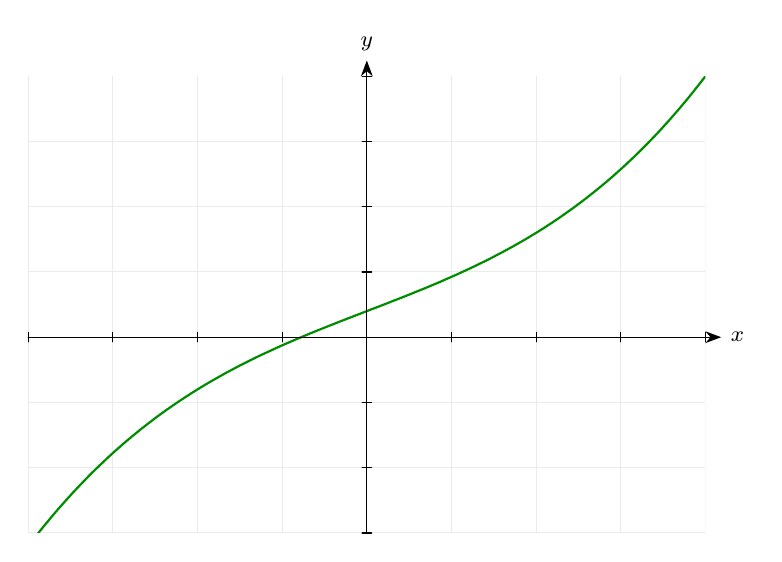
\begin{tikzpicture}[>={Stealth[length=2mm]},font=\footnotesize,line cap=round,line join=round]
\begin{scope}
\clip (0,0) rectangle (8.6,5.8);
\draw[gray!16] (0,0) grid[xstep=1.075,ystep=0.829] (8.6,5.8);
\draw[green!55!black,thick] (0,-0.166) -- (0.048,-0.104) -- (0.096,-0.042) -- (0.143,0.018) -- (0.191,0.077) -- (0.239,0.135) -- (0.287,0.193) -- (0.334,0.249) -- (0.382,0.305) -- (0.43,0.359) -- (0.478,0.413) -- (0.526,0.466) -- (0.573,0.518) -- (0.621,0.569) -- (0.669,0.619) -- (0.717,0.669) -- (0.764,0.718) -- (0.812,0.766) -- (0.86,0.813) -- (0.908,0.859) -- (0.956,0.904) -- (1.003,0.949) -- (1.051,0.993) -- (1.099,1.037) -- (1.147,1.079) -- (1.194,1.121) -- (1.242,1.162) -- (1.29,1.202) -- (1.338,1.242) -- (1.386,1.281) -- (1.433,1.32) -- (1.481,1.357) -- (1.529,1.394) -- (1.577,1.431) -- (1.624,1.467) -- (1.672,1.502) -- (1.72,1.537) -- (1.768,1.571) -- (1.816,1.604) -- (1.863,1.637) -- (1.911,1.669) -- (1.959,1.701) -- (2.007,1.732) -- (2.054,1.763) -- (2.102,1.793) -- (2.15,1.823) -- (2.198,1.852) -- (2.246,1.881) -- (2.293,1.909) -- (2.341,1.937) -- (2.389,1.964) -- (2.437,1.991) -- (2.484,2.018) -- (2.532,2.044) -- (2.58,2.069) -- (2.628,2.095) -- (2.676,2.12) -- (2.723,2.144) -- (2.771,2.168) -- (2.819,2.192) -- (2.867,2.216) -- (2.914,2.239) -- (2.962,2.262) -- (3.01,2.284) -- (3.058,2.306) -- (3.106,2.328) -- (3.153,2.35) -- (3.201,2.372) -- (3.249,2.393) -- (3.297,2.414) -- (3.344,2.434) -- (3.392,2.455) -- (3.44,2.475) -- (3.488,2.495) -- (3.536,2.515) -- (3.583,2.535) -- (3.631,2.554) -- (3.679,2.574) -- (3.727,2.593) -- (3.774,2.612) -- (3.822,2.631) -- (3.87,2.65) -- (3.918,2.669) -- (3.966,2.688) -- (4.013,2.706) -- (4.061,2.725) -- (4.109,2.743) -- (4.157,2.762) -- (4.204,2.78) -- (4.252,2.799) -- (4.3,2.817) -- (4.348,2.836) -- (4.396,2.854) -- (4.443,2.872) -- (4.491,2.891) -- (4.539,2.909) -- (4.587,2.928) -- (4.634,2.947) -- (4.682,2.965) -- (4.73,2.984) -- (4.778,3.003) -- (4.826,3.022) -- (4.873,3.041) -- (4.921,3.061) -- (4.969,3.08) -- (5.017,3.099) -- (5.064,3.119) -- (5.112,3.139) -- (5.16,3.159) -- (5.208,3.179) -- (5.256,3.2) -- (5.303,3.221) -- (5.351,3.242) -- (5.399,3.263) -- (5.447,3.284) -- (5.494,3.306) -- (5.542,3.328) -- (5.59,3.35) -- (5.638,3.373) -- (5.686,3.395) -- (5.733,3.419) -- (5.781,3.442) -- (5.829,3.466) -- (5.877,3.49) -- (5.924,3.515) -- (5.972,3.54) -- (6.02,3.565) -- (6.068,3.591) -- (6.116,3.617) -- (6.163,3.643) -- (6.211,3.67) -- (6.259,3.697) -- (6.307,3.725) -- (6.354,3.753) -- (6.402,3.782) -- (6.45,3.811) -- (6.498,3.841) -- (6.546,3.871) -- (6.593,3.902) -- (6.641,3.933) -- (6.689,3.965) -- (6.737,3.997) -- (6.784,4.03) -- (6.832,4.064) -- (6.88,4.098) -- (6.928,4.132) -- (6.976,4.168) -- (7.023,4.203) -- (7.071,4.24) -- (7.119,4.277) -- (7.167,4.315) -- (7.214,4.353) -- (7.262,4.392) -- (7.31,4.432) -- (7.358,4.472) -- (7.406,4.513) -- (7.453,4.555) -- (7.501,4.598) -- (7.549,4.641) -- (7.597,4.685) -- (7.644,4.73) -- (7.692,4.775) -- (7.74,4.822) -- (7.788,4.869) -- (7.836,4.917) -- (7.883,4.965) -- (7.931,5.015) -- (7.979,5.065) -- (8.027,5.116) -- (8.074,5.168) -- (8.122,5.221) -- (8.17,5.275) -- (8.218,5.33) -- (8.266,5.385) -- (8.313,5.442) -- (8.361,5.499) -- (8.409,5.557) -- (8.457,5.617) -- (8.504,5.677) -- (8.552,5.738) -- (8.6,5.8);
\end{scope}
\draw[->] (0,2.486) -- (8.8,2.486) node[right]{$x$};
\draw[->] (4.3,0) -- (4.3,6) node[above]{$y$};
\draw (0,2.426) -- (0,2.546);
\draw (1.075,2.426) -- (1.075,2.546);
\draw (2.15,2.426) -- (2.15,2.546);
\draw (3.225,2.426) -- (3.225,2.546);
\draw (5.375,2.426) -- (5.375,2.546);
\draw (6.45,2.426) -- (6.45,2.546);
\draw (7.525,2.426) -- (7.525,2.546);
\draw (8.6,2.426) -- (8.6,2.546);
\draw (4.24,0) -- (4.36,0);
\draw (4.24,0.829) -- (4.36,0.829);
\draw (4.24,1.657) -- (4.36,1.657);
\draw (4.24,3.314) -- (4.36,3.314);
\draw (4.24,4.143) -- (4.36,4.143);
\draw (4.24,4.971) -- (4.36,4.971);
\draw (4.24,5.8) -- (4.36,5.8);
\end{tikzpicture}
}
\end{center}
\small Curve coloured green where increasing, red where decreasing.\normalsize

\medskip\hrule

\section*{Derivatives and Graphs 08\quad\small\texttt{(d4-008)}}
\addcontentsline{toc}{section}{Derivatives and Graphs 08 (d4-008)}
\textit{Difficulty: Foundation \quad\textbar\quad Marks: 4}

\question{A function is given by \( f(x) = x^3 + kx \), where \( k \) is a constant. Given that \( f(x) \) has no stationary points, find the range of values of \( k \).}

\textbf{Worked solution.}

\textit{Step 1: Differentiate.}
\[\begin{gathered}
f'(x) = 3x^2 + k
\end{gathered}\]
Power rule.

\textit{Step 2: For no stationary points, \( f'(x) > 0 \) for all \( x \).}
\[\begin{gathered}
3x^2 + k > 0 \text{ for all } x
\end{gathered}\]
The minimum value of \( 3x^2 \) is \(0\) (at \( x = 0 \)), so we need \( k > 0 \).

\textit{Step 3: State the condition.}
\[\begin{gathered}
k > 0
\end{gathered}\]
If \( k > 0 \), then \( f'(x) = 3x^2 + k \geq k > 0 \) for all \( x \).

\begin{answerbox}
\textbf{Final answer:}\quad \(\displaystyle  k > 0 \)
\end{answerbox}
\textbf{Diagram.}

\begin{center}
\resizebox{\ifdim\width>\linewidth \linewidth\else \width\fi}{!}{%
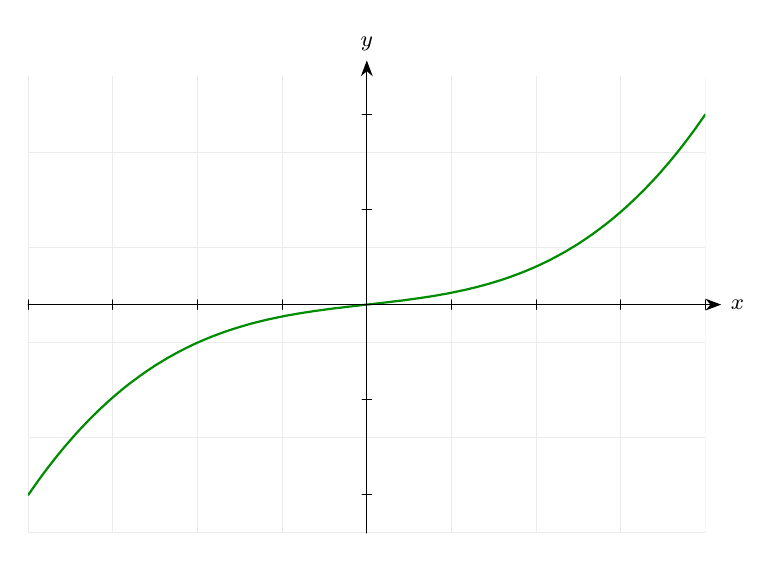
\begin{tikzpicture}[>={Stealth[length=2mm]},font=\footnotesize,line cap=round,line join=round]
\begin{scope}
\clip (0,0) rectangle (8.6,5.8);
\draw[gray!16] (0,-0.725) grid[xstep=1.075,ystep=1.208] (8.6,5.8);
\draw[green!55!black,thick] (0,0.483) -- (0.048,0.552) -- (0.096,0.62) -- (0.143,0.686) -- (0.191,0.751) -- (0.239,0.815) -- (0.287,0.877) -- (0.334,0.938) -- (0.382,0.997) -- (0.43,1.056) -- (0.478,1.113) -- (0.526,1.168) -- (0.573,1.223) -- (0.621,1.276) -- (0.669,1.328) -- (0.717,1.378) -- (0.764,1.428) -- (0.812,1.476) -- (0.86,1.523) -- (0.908,1.57) -- (0.956,1.614) -- (1.003,1.658) -- (1.051,1.701) -- (1.099,1.743) -- (1.147,1.783) -- (1.194,1.823) -- (1.242,1.861) -- (1.29,1.899) -- (1.338,1.935) -- (1.386,1.97) -- (1.433,2.005) -- (1.481,2.038) -- (1.529,2.071) -- (1.577,2.103) -- (1.624,2.134) -- (1.672,2.163) -- (1.72,2.192) -- (1.768,2.221) -- (1.816,2.248) -- (1.863,2.274) -- (1.911,2.3) -- (1.959,2.325) -- (2.007,2.349) -- (2.054,2.372) -- (2.102,2.395) -- (2.15,2.417) -- (2.198,2.438) -- (2.246,2.458) -- (2.293,2.478) -- (2.341,2.497) -- (2.389,2.515) -- (2.437,2.533) -- (2.484,2.55) -- (2.532,2.567) -- (2.58,2.583) -- (2.628,2.598) -- (2.676,2.613) -- (2.723,2.627) -- (2.771,2.641) -- (2.819,2.655) -- (2.867,2.667) -- (2.914,2.68) -- (2.962,2.691) -- (3.01,2.703) -- (3.058,2.714) -- (3.106,2.724) -- (3.153,2.734) -- (3.201,2.744) -- (3.249,2.754) -- (3.297,2.763) -- (3.344,2.771) -- (3.392,2.78) -- (3.44,2.788) -- (3.488,2.796) -- (3.536,2.803) -- (3.583,2.81) -- (3.631,2.818) -- (3.679,2.824) -- (3.727,2.831) -- (3.774,2.837) -- (3.822,2.844) -- (3.87,2.85) -- (3.918,2.856) -- (3.966,2.861) -- (4.013,2.867) -- (4.061,2.873) -- (4.109,2.878) -- (4.157,2.884) -- (4.204,2.889) -- (4.252,2.895) -- (4.3,2.9) -- (4.348,2.905) -- (4.396,2.911) -- (4.443,2.916) -- (4.491,2.922) -- (4.539,2.927) -- (4.587,2.933) -- (4.634,2.939) -- (4.682,2.944) -- (4.73,2.95) -- (4.778,2.956) -- (4.826,2.963) -- (4.873,2.969) -- (4.921,2.976) -- (4.969,2.982) -- (5.017,2.99) -- (5.064,2.997) -- (5.112,3.004) -- (5.16,3.012) -- (5.208,3.02) -- (5.256,3.029) -- (5.303,3.037) -- (5.351,3.046) -- (5.399,3.056) -- (5.447,3.066) -- (5.494,3.076) -- (5.542,3.086) -- (5.59,3.097) -- (5.638,3.109) -- (5.686,3.12) -- (5.733,3.133) -- (5.781,3.145) -- (5.829,3.159) -- (5.877,3.173) -- (5.924,3.187) -- (5.972,3.202) -- (6.02,3.217) -- (6.068,3.233) -- (6.116,3.25) -- (6.163,3.267) -- (6.211,3.285) -- (6.259,3.303) -- (6.307,3.322) -- (6.354,3.342) -- (6.402,3.362) -- (6.45,3.383) -- (6.498,3.405) -- (6.546,3.428) -- (6.593,3.451) -- (6.641,3.475) -- (6.689,3.5) -- (6.737,3.526) -- (6.784,3.552) -- (6.832,3.579) -- (6.88,3.608) -- (6.928,3.637) -- (6.976,3.666) -- (7.023,3.697) -- (7.071,3.729) -- (7.119,3.762) -- (7.167,3.795) -- (7.214,3.83) -- (7.262,3.865) -- (7.31,3.901) -- (7.358,3.939) -- (7.406,3.977) -- (7.453,4.017) -- (7.501,4.057) -- (7.549,4.099) -- (7.597,4.142) -- (7.644,4.186) -- (7.692,4.23) -- (7.74,4.277) -- (7.788,4.324) -- (7.836,4.372) -- (7.883,4.422) -- (7.931,4.472) -- (7.979,4.524) -- (8.027,4.577) -- (8.074,4.632) -- (8.122,4.687) -- (8.17,4.744) -- (8.218,4.803) -- (8.266,4.862) -- (8.313,4.923) -- (8.361,4.985) -- (8.409,5.049) -- (8.457,5.114) -- (8.504,5.18) -- (8.552,5.248) -- (8.6,5.317);
\end{scope}
\draw[->] (0,2.9) -- (8.8,2.9) node[right]{$x$};
\draw[->] (4.3,0) -- (4.3,6) node[above]{$y$};
\draw (0,2.84) -- (0,2.96);
\draw (1.075,2.84) -- (1.075,2.96);
\draw (2.15,2.84) -- (2.15,2.96);
\draw (3.225,2.84) -- (3.225,2.96);
\draw (5.375,2.84) -- (5.375,2.96);
\draw (6.45,2.84) -- (6.45,2.96);
\draw (7.525,2.84) -- (7.525,2.96);
\draw (8.6,2.84) -- (8.6,2.96);
\draw (4.24,0.483) -- (4.36,0.483);
\draw (4.24,1.692) -- (4.36,1.692);
\draw (4.24,4.108) -- (4.36,4.108);
\draw (4.24,5.317) -- (4.36,5.317);
\end{tikzpicture}
}
\end{center}
\small Curve coloured green where increasing, red where decreasing.\normalsize

\medskip\hrule

\section*{Derivatives and Graphs 09\quad\small\texttt{(d4-009)}}
\addcontentsline{toc}{section}{Derivatives and Graphs 09 (d4-009)}
\textit{Difficulty: Foundation \quad\textbar\quad Marks: 6}

\question{Find the coordinates of the stationary points of \( y = x^4 - 8x^2 + 5 \) and classify them.}

\textbf{Worked solution.}

\textit{Step 1: Differentiate.}
\[\begin{gathered}
\frac{\mathrm{d}y}{\mathrm{d}x} = 4x^3 - 16x
\end{gathered}\]
Power rule.

\textit{Step 2: Solve \( 4x^3 - 16x = 0 \).}
\[\begin{gathered}
4x(x^2 - 4) = 0 \implies x = 0,\; x = 2,\; x = -2
\end{gathered}\]
Factorise \( 4x(x-2)(x+2) = 0 \).

\textit{Step 3: Find \( y \)-coordinates.}
\[\begin{gathered}
y(0) = 5; \quad y(2) = 16 - 32 + 5 = -11; \quad y(-2) = -11
\end{gathered}\]
Substitute into \( y = x^4 - 8x^2 + 5 \).

\textit{Step 4: Second derivative.}
\[\begin{gathered}
\frac{\mathrm{d}^2y}{\mathrm{d}x^2} = 12x^2 - 16
\end{gathered}\]
Differentiate the first derivative.

\textit{Step 5: Classify.}
\[\begin{gathered}
x=0: -16 < 0 \Rightarrow \text{maximum} \newline x=\pm2: 48 - 16 = 32 > 0 \Rightarrow \text{minima}
\end{gathered}\]
Substitute each \( x \)-value into \( \dfrac{\mathrm{d}^2y}{\mathrm{d}x^2} \).

\begin{answerbox}
\textbf{Final answer:}\quad Local maximum at \(\displaystyle  (0, 5) \); local minima at \(\displaystyle  (2, -11) \) and \(\displaystyle  (-2, -11) \)
\end{answerbox}
\textbf{Diagram.}

\begin{center}
\resizebox{\ifdim\width>\linewidth \linewidth\else \width\fi}{!}{%
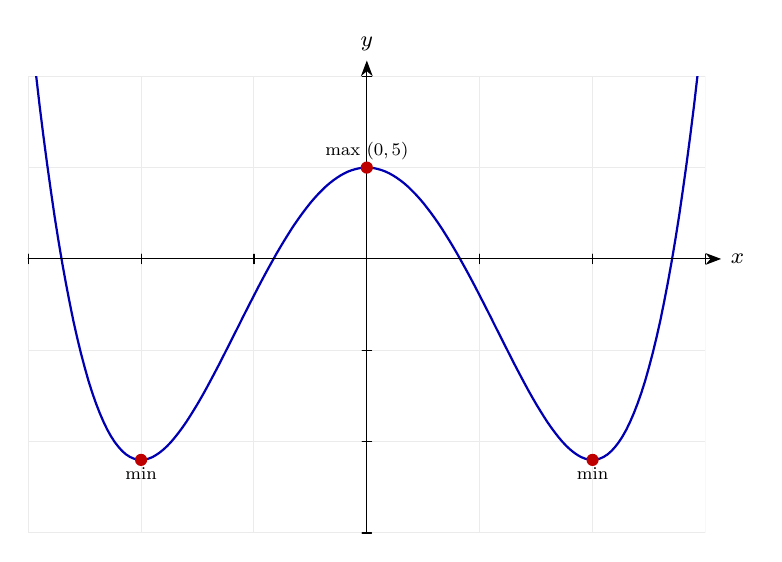
\begin{tikzpicture}[>={Stealth[length=2mm]},font=\footnotesize,line cap=round,line join=round]
\begin{scope}
\clip (0,0) rectangle (8.6,5.8);
\draw[gray!16] (0,0) grid[xstep=1.433,ystep=1.16] (8.6,5.8);
\draw[blue!70!black,thick] (0,6.728) -- (0.048,6.276) -- (0.096,5.847) -- (0.143,5.44) -- (0.191,5.055) -- (0.239,4.692) -- (0.287,4.349) -- (0.334,4.026) -- (0.382,3.723) -- (0.43,3.439) -- (0.478,3.174) -- (0.526,2.926) -- (0.573,2.695) -- (0.621,2.482) -- (0.669,2.284) -- (0.717,2.103) -- (0.764,1.936) -- (0.812,1.784) -- (0.86,1.647) -- (0.908,1.523) -- (0.956,1.412) -- (1.003,1.314) -- (1.051,1.228) -- (1.099,1.154) -- (1.147,1.092) -- (1.194,1.04) -- (1.242,0.998) -- (1.29,0.967) -- (1.338,0.945) -- (1.386,0.932) -- (1.433,0.928) -- (1.481,0.932) -- (1.529,0.944) -- (1.577,0.963) -- (1.624,0.99) -- (1.672,1.023) -- (1.72,1.062) -- (1.768,1.107) -- (1.816,1.158) -- (1.863,1.214) -- (1.911,1.275) -- (1.959,1.34) -- (2.007,1.409) -- (2.054,1.482) -- (2.102,1.559) -- (2.15,1.638) -- (2.198,1.721) -- (2.246,1.806) -- (2.293,1.893) -- (2.341,1.983) -- (2.389,2.074) -- (2.437,2.166) -- (2.484,2.259) -- (2.532,2.354) -- (2.58,2.448) -- (2.628,2.544) -- (2.676,2.639) -- (2.723,2.734) -- (2.771,2.829) -- (2.819,2.923) -- (2.867,3.016) -- (2.914,3.108) -- (2.962,3.199) -- (3.01,3.289) -- (3.058,3.377) -- (3.106,3.463) -- (3.153,3.547) -- (3.201,3.629) -- (3.249,3.709) -- (3.297,3.786) -- (3.344,3.861) -- (3.392,3.933) -- (3.44,4.002) -- (3.488,4.068) -- (3.536,4.131) -- (3.583,4.191) -- (3.631,4.247) -- (3.679,4.3) -- (3.727,4.349) -- (3.774,4.395) -- (3.822,4.437) -- (3.87,4.475) -- (3.918,4.509) -- (3.966,4.54) -- (4.013,4.566) -- (4.061,4.589) -- (4.109,4.607) -- (4.157,4.621) -- (4.204,4.632) -- (4.252,4.638) -- (4.3,4.64) -- (4.348,4.638) -- (4.396,4.632) -- (4.443,4.621) -- (4.491,4.607) -- (4.539,4.589) -- (4.587,4.566) -- (4.634,4.54) -- (4.682,4.509) -- (4.73,4.475) -- (4.778,4.437) -- (4.826,4.395) -- (4.873,4.349) -- (4.921,4.3) -- (4.969,4.247) -- (5.017,4.191) -- (5.064,4.131) -- (5.112,4.068) -- (5.16,4.002) -- (5.208,3.933) -- (5.256,3.861) -- (5.303,3.786) -- (5.351,3.709) -- (5.399,3.629) -- (5.447,3.547) -- (5.494,3.463) -- (5.542,3.377) -- (5.59,3.289) -- (5.638,3.199) -- (5.686,3.108) -- (5.733,3.016) -- (5.781,2.923) -- (5.829,2.829) -- (5.877,2.734) -- (5.924,2.639) -- (5.972,2.544) -- (6.02,2.448) -- (6.068,2.354) -- (6.116,2.259) -- (6.163,2.166) -- (6.211,2.074) -- (6.259,1.983) -- (6.307,1.893) -- (6.354,1.806) -- (6.402,1.721) -- (6.45,1.638) -- (6.498,1.559) -- (6.546,1.482) -- (6.593,1.409) -- (6.641,1.34) -- (6.689,1.275) -- (6.737,1.214) -- (6.784,1.158) -- (6.832,1.107) -- (6.88,1.062) -- (6.928,1.023) -- (6.976,0.99) -- (7.023,0.963) -- (7.071,0.944) -- (7.119,0.932) -- (7.167,0.928) -- (7.214,0.932) -- (7.262,0.945) -- (7.31,0.967) -- (7.358,0.998) -- (7.406,1.04) -- (7.453,1.092) -- (7.501,1.154) -- (7.549,1.228) -- (7.597,1.314) -- (7.644,1.412) -- (7.692,1.523) -- (7.74,1.647) -- (7.788,1.784) -- (7.836,1.936) -- (7.883,2.103) -- (7.931,2.284) -- (7.979,2.482) -- (8.027,2.695) -- (8.074,2.926) -- (8.122,3.174) -- (8.17,3.439) -- (8.218,3.723) -- (8.266,4.026) -- (8.313,4.349) -- (8.361,4.692) -- (8.409,5.055) -- (8.457,5.44) -- (8.504,5.847) -- (8.552,6.276) -- (8.6,6.728);
\end{scope}
\draw[->] (0,3.48) -- (8.8,3.48) node[right]{$x$};
\draw[->] (4.3,0) -- (4.3,6) node[above]{$y$};
\draw (0,3.42) -- (0,3.54);
\draw (1.433,3.42) -- (1.433,3.54);
\draw (2.867,3.42) -- (2.867,3.54);
\draw (5.733,3.42) -- (5.733,3.54);
\draw (7.167,3.42) -- (7.167,3.54);
\draw (8.6,3.42) -- (8.6,3.54);
\draw (4.24,0) -- (4.36,0);
\draw (4.24,1.16) -- (4.36,1.16);
\draw (4.24,2.32) -- (4.36,2.32);
\draw (4.24,4.64) -- (4.36,4.64);
\draw (4.24,5.8) -- (4.36,5.8);
\fill[red!75!black] (4.3,4.64) circle (2.2pt);
\node[above,scale=0.8] at (4.3,4.64) {max $(0,5)$};
\fill[red!75!black] (7.167,0.928) circle (2.2pt);
\node[below,scale=0.8] at (7.167,0.928) {min};
\fill[red!75!black] (1.433,0.928) circle (2.2pt);
\node[below,scale=0.8] at (1.433,0.928) {min};
\end{tikzpicture}
}
\end{center}
\small Curve with classified stationary points marked.\normalsize

\medskip\hrule

\section*{Derivatives and Graphs 10\quad\small\texttt{(d4-010)}}
\addcontentsline{toc}{section}{Derivatives and Graphs 10 (d4-010)}
\textit{Difficulty: Foundation \quad\textbar\quad Marks: 3}

\question{Find the values of \( x \) for which \( y = x^2 - 6x + 5 \) is an increasing function.}

\textbf{Worked solution.}

\textit{Step 1: Differentiate.}
\[\begin{gathered}
\frac{\mathrm{d}y}{\mathrm{d}x} = 2x - 6
\end{gathered}\]
Power rule.

\textit{Step 2: The function is increasing when the derivative is positive.}
\[\begin{gathered}
2x - 6 > 0 \implies x > 3
\end{gathered}\]
Solve the linear inequality.

\begin{answerbox}
\textbf{Final answer:}\quad \(\displaystyle  x > 3 \)
\end{answerbox}
\textbf{Diagram.}

\begin{center}
\resizebox{\ifdim\width>\linewidth \linewidth\else \width\fi}{!}{%
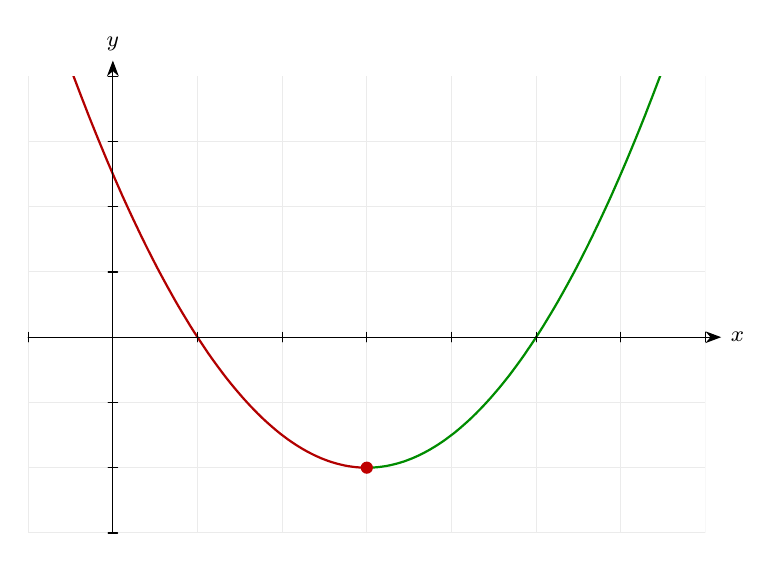
\begin{tikzpicture}[>={Stealth[length=2mm]},font=\footnotesize,line cap=round,line join=round]
\begin{scope}
\clip (0,0) rectangle (8.6,5.8);
\draw[gray!16] (0,0) grid[xstep=1.075,ystep=0.829] (8.6,5.8);
\draw[red!70!black,thick] (0,7.457) -- (0.048,7.311) -- (0.096,7.166) -- (0.143,7.023) -- (0.191,6.881) -- (0.239,6.741) -- (0.287,6.603) -- (0.334,6.466) -- (0.382,6.331) -- (0.43,6.198) -- (0.478,6.066) -- (0.526,5.936) -- (0.573,5.807) -- (0.621,5.681) -- (0.669,5.555) -- (0.717,5.432) -- (0.764,5.31) -- (0.812,5.19) -- (0.86,5.071) -- (0.908,4.954) -- (0.956,4.838) -- (1.003,4.725) -- (1.051,4.613) -- (1.099,4.502) -- (1.147,4.393) -- (1.194,4.286) -- (1.242,4.181) -- (1.29,4.077) -- (1.338,3.974) -- (1.386,3.874) -- (1.433,3.775) -- (1.481,3.677) -- (1.529,3.581) -- (1.577,3.487) -- (1.624,3.395) -- (1.672,3.304) -- (1.72,3.215) -- (1.768,3.127) -- (1.816,3.041) -- (1.863,2.957) -- (1.911,2.874) -- (1.959,2.793) -- (2.007,2.714) -- (2.054,2.636) -- (2.102,2.56) -- (2.15,2.486) -- (2.198,2.413) -- (2.246,2.342) -- (2.293,2.272) -- (2.341,2.204) -- (2.389,2.138) -- (2.437,2.073) -- (2.484,2.01) -- (2.532,1.949) -- (2.58,1.889) -- (2.628,1.831) -- (2.676,1.775) -- (2.723,1.72) -- (2.771,1.667) -- (2.819,1.615) -- (2.867,1.565) -- (2.914,1.517) -- (2.962,1.47) -- (3.01,1.425) -- (3.058,1.382) -- (3.106,1.34) -- (3.153,1.3) -- (3.201,1.261) -- (3.249,1.225) -- (3.297,1.189) -- (3.344,1.156) -- (3.392,1.124) -- (3.44,1.094) -- (3.488,1.065) -- (3.536,1.038) -- (3.583,1.013) -- (3.631,0.989) -- (3.679,0.967) -- (3.727,0.946) -- (3.774,0.928) -- (3.822,0.91) -- (3.87,0.895) -- (3.918,0.881) -- (3.966,0.869) -- (4.013,0.858) -- (4.061,0.849) -- (4.109,0.842) -- (4.157,0.836) -- (4.204,0.832) -- (4.252,0.829) -- (4.3,0.829);
\draw[green!55!black,thick] (4.3,0.829) -- (4.348,0.829) -- (4.396,0.832) -- (4.443,0.836) -- (4.491,0.842) -- (4.539,0.849) -- (4.587,0.858) -- (4.634,0.869) -- (4.682,0.881) -- (4.73,0.895) -- (4.778,0.91) -- (4.826,0.928) -- (4.873,0.946) -- (4.921,0.967) -- (4.969,0.989) -- (5.017,1.013) -- (5.064,1.038) -- (5.112,1.065) -- (5.16,1.094) -- (5.208,1.124) -- (5.256,1.156) -- (5.303,1.189) -- (5.351,1.225) -- (5.399,1.261) -- (5.447,1.3) -- (5.494,1.34) -- (5.542,1.382) -- (5.59,1.425) -- (5.638,1.47) -- (5.686,1.517) -- (5.733,1.565) -- (5.781,1.615) -- (5.829,1.667) -- (5.877,1.72) -- (5.924,1.775) -- (5.972,1.831) -- (6.02,1.889) -- (6.068,1.949) -- (6.116,2.01) -- (6.163,2.073) -- (6.211,2.138) -- (6.259,2.204) -- (6.307,2.272) -- (6.354,2.342) -- (6.402,2.413) -- (6.45,2.486) -- (6.498,2.56) -- (6.546,2.636) -- (6.593,2.714) -- (6.641,2.793) -- (6.689,2.874) -- (6.737,2.957) -- (6.784,3.041) -- (6.832,3.127) -- (6.88,3.215) -- (6.928,3.304) -- (6.976,3.395) -- (7.023,3.487) -- (7.071,3.581) -- (7.119,3.677) -- (7.167,3.775) -- (7.214,3.874) -- (7.262,3.974) -- (7.31,4.077) -- (7.358,4.181) -- (7.406,4.286) -- (7.453,4.393) -- (7.501,4.502) -- (7.549,4.613) -- (7.597,4.725) -- (7.644,4.838) -- (7.692,4.954) -- (7.74,5.071) -- (7.788,5.19) -- (7.836,5.31) -- (7.883,5.432) -- (7.931,5.555) -- (7.979,5.681) -- (8.027,5.807) -- (8.074,5.936) -- (8.122,6.066) -- (8.17,6.198) -- (8.218,6.331) -- (8.266,6.466) -- (8.313,6.603) -- (8.361,6.741) -- (8.409,6.881) -- (8.457,7.023) -- (8.504,7.166) -- (8.552,7.311) -- (8.6,7.457);
\end{scope}
\draw[->] (0,2.486) -- (8.8,2.486) node[right]{$x$};
\draw[->] (1.075,0) -- (1.075,6) node[above]{$y$};
\draw (0,2.426) -- (0,2.546);
\draw (2.15,2.426) -- (2.15,2.546);
\draw (3.225,2.426) -- (3.225,2.546);
\draw (4.3,2.426) -- (4.3,2.546);
\draw (5.375,2.426) -- (5.375,2.546);
\draw (6.45,2.426) -- (6.45,2.546);
\draw (7.525,2.426) -- (7.525,2.546);
\draw (8.6,2.426) -- (8.6,2.546);
\draw (1.015,0) -- (1.135,0);
\draw (1.015,0.829) -- (1.135,0.829);
\draw (1.015,1.657) -- (1.135,1.657);
\draw (1.015,3.314) -- (1.135,3.314);
\draw (1.015,4.143) -- (1.135,4.143);
\draw (1.015,4.971) -- (1.135,4.971);
\draw (1.015,5.8) -- (1.135,5.8);
\fill[red!75!black] (4.3,0.829) circle (2.2pt);
\end{tikzpicture}
}
\end{center}
\small Curve coloured green where increasing, red where decreasing.\normalsize

\medskip\hrule

\section*{Derivatives and Graphs 11\quad\small\texttt{(d4-011)}}
\addcontentsline{toc}{section}{Derivatives and Graphs 11 (d4-011)}
\textit{Difficulty: Foundation \quad\textbar\quad Marks: 3}

\question{Find the values of \( x \) for which \( y = x^2 + 4x - 3 \) is a decreasing function.}

\textbf{Worked solution.}

\textit{Step 1: Differentiate.}
\[\begin{gathered}
\frac{\mathrm{d}y}{\mathrm{d}x} = 2x + 4
\end{gathered}\]
Power rule.

\textit{Step 2: The function is decreasing when the derivative is negative.}
\[\begin{gathered}
2x + 4 < 0 \implies x < -2
\end{gathered}\]
Solve the linear inequality.

\begin{answerbox}
\textbf{Final answer:}\quad \(\displaystyle  x < -2 \)
\end{answerbox}
\textbf{Diagram.}

\begin{center}
\resizebox{\ifdim\width>\linewidth \linewidth\else \width\fi}{!}{%
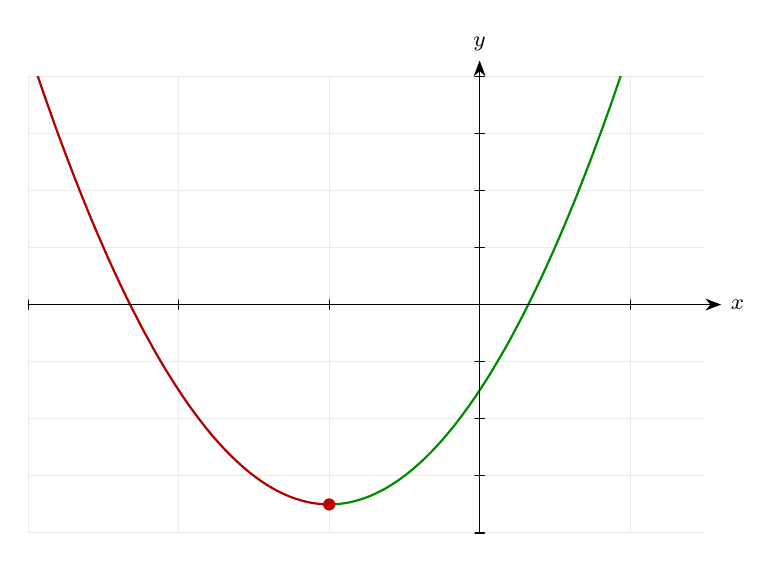
\begin{tikzpicture}[>={Stealth[length=2mm]},font=\footnotesize,line cap=round,line join=round]
\begin{scope}
\clip (0,0) rectangle (8.6,5.8);
\draw[gray!16] (0,0) grid[xstep=1.911,ystep=0.725] (8.6,5.8);
\draw[red!70!black,thick] (0,6.162) -- (0.048,6.018) -- (0.096,5.876) -- (0.143,5.736) -- (0.191,5.597) -- (0.239,5.46) -- (0.287,5.325) -- (0.334,5.192) -- (0.382,5.06) -- (0.43,4.931) -- (0.478,4.803) -- (0.526,4.677) -- (0.573,4.553) -- (0.621,4.431) -- (0.669,4.31) -- (0.717,4.191) -- (0.764,4.075) -- (0.812,3.959) -- (0.86,3.846) -- (0.908,3.735) -- (0.956,3.625) -- (1.003,3.517) -- (1.051,3.411) -- (1.099,3.307) -- (1.147,3.204) -- (1.194,3.104) -- (1.242,3.005) -- (1.29,2.908) -- (1.338,2.813) -- (1.386,2.72) -- (1.433,2.628) -- (1.481,2.538) -- (1.529,2.451) -- (1.577,2.364) -- (1.624,2.28) -- (1.672,2.198) -- (1.72,2.117) -- (1.768,2.038) -- (1.816,1.961) -- (1.863,1.886) -- (1.911,1.813) -- (1.959,1.741) -- (2.007,1.671) -- (2.054,1.603) -- (2.102,1.537) -- (2.15,1.473) -- (2.198,1.41) -- (2.246,1.349) -- (2.293,1.291) -- (2.341,1.233) -- (2.389,1.178) -- (2.437,1.125) -- (2.484,1.073) -- (2.532,1.023) -- (2.58,0.975) -- (2.628,0.929) -- (2.676,0.885) -- (2.723,0.842) -- (2.771,0.801) -- (2.819,0.762) -- (2.867,0.725) -- (2.914,0.69) -- (2.962,0.656) -- (3.01,0.624) -- (3.058,0.594) -- (3.106,0.566) -- (3.153,0.54) -- (3.201,0.516) -- (3.249,0.493) -- (3.297,0.472) -- (3.344,0.453) -- (3.392,0.436) -- (3.44,0.421) -- (3.488,0.407) -- (3.536,0.395) -- (3.583,0.385) -- (3.631,0.377) -- (3.679,0.371) -- (3.727,0.366) -- (3.774,0.363) -- (3.822,0.362);
\draw[green!55!black,thick] (3.822,0.362) -- (3.87,0.363) -- (3.918,0.366) -- (3.966,0.371) -- (4.013,0.377) -- (4.061,0.385) -- (4.109,0.395) -- (4.157,0.407) -- (4.204,0.421) -- (4.252,0.436) -- (4.3,0.453) -- (4.348,0.472) -- (4.396,0.493) -- (4.443,0.516) -- (4.491,0.54) -- (4.539,0.566) -- (4.587,0.595) -- (4.634,0.624) -- (4.682,0.656) -- (4.73,0.69) -- (4.778,0.725) -- (4.826,0.762) -- (4.873,0.801) -- (4.921,0.842) -- (4.969,0.884) -- (5.017,0.929) -- (5.064,0.975) -- (5.112,1.023) -- (5.16,1.073) -- (5.208,1.125) -- (5.256,1.178) -- (5.303,1.233) -- (5.351,1.291) -- (5.399,1.349) -- (5.447,1.41) -- (5.494,1.473) -- (5.542,1.537) -- (5.59,1.603) -- (5.638,1.671) -- (5.686,1.741) -- (5.733,1.813) -- (5.781,1.886) -- (5.829,1.961) -- (5.877,2.038) -- (5.924,2.117) -- (5.972,2.198) -- (6.02,2.28) -- (6.068,2.364) -- (6.116,2.45) -- (6.163,2.538) -- (6.211,2.628) -- (6.259,2.72) -- (6.307,2.813) -- (6.354,2.908) -- (6.402,3.005) -- (6.45,3.104) -- (6.498,3.205) -- (6.546,3.307) -- (6.593,3.411) -- (6.641,3.517) -- (6.689,3.625) -- (6.737,3.735) -- (6.784,3.846) -- (6.832,3.959) -- (6.88,4.075) -- (6.928,4.191) -- (6.976,4.31) -- (7.023,4.431) -- (7.071,4.553) -- (7.119,4.677) -- (7.167,4.803) -- (7.214,4.931) -- (7.262,5.06) -- (7.31,5.192) -- (7.358,5.325) -- (7.406,5.46) -- (7.453,5.597) -- (7.501,5.736) -- (7.549,5.876) -- (7.597,6.018) -- (7.644,6.162) -- (7.692,6.308) -- (7.74,6.456) -- (7.788,6.606) -- (7.836,6.757) -- (7.883,6.91) -- (7.931,7.065) -- (7.979,7.222) -- (8.027,7.381) -- (8.074,7.541) -- (8.122,7.703) -- (8.17,7.867) -- (8.218,8.033) -- (8.266,8.201) -- (8.313,8.37) -- (8.361,8.541) -- (8.409,8.714) -- (8.457,8.889) -- (8.504,9.066) -- (8.552,9.245) -- (8.6,9.425);
\end{scope}
\draw[->] (0,2.9) -- (8.8,2.9) node[right]{$x$};
\draw[->] (5.733,0) -- (5.733,6) node[above]{$y$};
\draw (0,2.84) -- (0,2.96);
\draw (1.911,2.84) -- (1.911,2.96);
\draw (3.822,2.84) -- (3.822,2.96);
\draw (7.644,2.84) -- (7.644,2.96);
\draw (5.673,0) -- (5.793,0);
\draw (5.673,0.725) -- (5.793,0.725);
\draw (5.673,1.45) -- (5.793,1.45);
\draw (5.673,2.175) -- (5.793,2.175);
\draw (5.673,3.625) -- (5.793,3.625);
\draw (5.673,4.35) -- (5.793,4.35);
\draw (5.673,5.075) -- (5.793,5.075);
\draw (5.673,5.8) -- (5.793,5.8);
\fill[red!75!black] (3.822,0.362) circle (2.2pt);
\end{tikzpicture}
}
\end{center}
\small Curve coloured green where increasing, red where decreasing.\normalsize

\medskip\hrule

\section*{Derivatives and Graphs 12\quad\small\texttt{(d4-012)}}
\addcontentsline{toc}{section}{Derivatives and Graphs 12 (d4-012)}
\textit{Difficulty: Foundation \quad\textbar\quad Marks: 4}

\question{Find the values of \( x \) for which \( f(x) = x^3 - 3x^2 - 9x + 2 \) is increasing.}

\textbf{Worked solution.}

\textit{Step 1: Differentiate.}
\[\begin{gathered}
f'(x) = 3x^2 - 6x - 9
\end{gathered}\]
Power rule.

\textit{Step 2: Form the inequality \( f'(x) > 0 \).}
\[\begin{gathered}
3x^2 - 6x - 9 > 0 \implies x^2 - 2x - 3 > 0 \implies (x - 3)(x + 1) > 0
\end{gathered}\]
Divide by 3 and factorise.

\textit{Step 3: Solve the quadratic inequality.}
\[\begin{gathered}
x < -1 \text{ or } x > 3
\end{gathered}\]
The product \( (x-3)(x+1) > 0 \) when both factors are positive or both are negative.

\begin{answerbox}
\textbf{Final answer:}\quad \(\displaystyle  x < -1 \) or \(\displaystyle  x > 3 \)
\end{answerbox}
\textbf{Diagram.}

\begin{center}
\resizebox{\ifdim\width>\linewidth \linewidth\else \width\fi}{!}{%
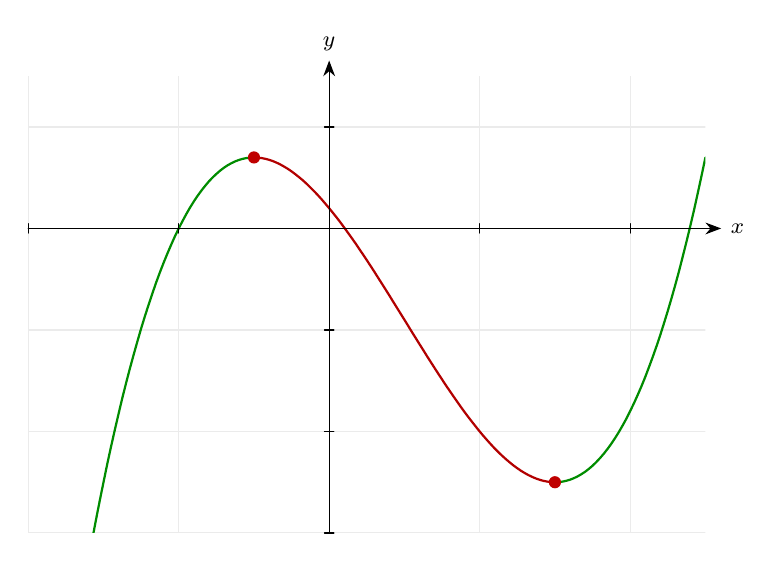
\begin{tikzpicture}[>={Stealth[length=2mm]},font=\footnotesize,line cap=round,line join=round]
\begin{scope}
\clip (0,0) rectangle (8.6,5.8);
\draw[gray!16] (0,0) grid[xstep=1.911,ystep=1.289] (8.6,5.8);
\draw[green!55!black,thick] (0,-5.671) -- (0.048,-5.27) -- (0.096,-4.878) -- (0.143,-4.496) -- (0.191,-4.123) -- (0.239,-3.76) -- (0.287,-3.406) -- (0.334,-3.06) -- (0.382,-2.724) -- (0.43,-2.397) -- (0.478,-2.078) -- (0.526,-1.769) -- (0.573,-1.467) -- (0.621,-1.175) -- (0.669,-0.89) -- (0.717,-0.614) -- (0.764,-0.346) -- (0.812,-0.087) -- (0.86,0.165) -- (0.908,0.409) -- (0.956,0.644) -- (1.003,0.873) -- (1.051,1.093) -- (1.099,1.306) -- (1.147,1.512) -- (1.194,1.71) -- (1.242,1.901) -- (1.29,2.085) -- (1.338,2.261) -- (1.386,2.431) -- (1.433,2.594) -- (1.481,2.75) -- (1.529,2.899) -- (1.577,3.042) -- (1.624,3.179) -- (1.672,3.309) -- (1.72,3.433) -- (1.768,3.55) -- (1.816,3.662) -- (1.863,3.767) -- (1.911,3.867) -- (1.959,3.96) -- (2.007,4.049) -- (2.054,4.131) -- (2.102,4.208) -- (2.15,4.28) -- (2.198,4.346) -- (2.246,4.407) -- (2.293,4.463) -- (2.341,4.514) -- (2.389,4.559) -- (2.437,4.601) -- (2.484,4.637) -- (2.532,4.669) -- (2.58,4.696) -- (2.628,4.719) -- (2.676,4.737) -- (2.723,4.751) -- (2.771,4.761) -- (2.819,4.767) -- (2.867,4.769);
\draw[red!70!black,thick] (2.867,4.769) -- (2.914,4.767) -- (2.962,4.761) -- (3.01,4.752) -- (3.058,4.739) -- (3.106,4.723) -- (3.153,4.703) -- (3.201,4.68) -- (3.249,4.653) -- (3.297,4.624) -- (3.344,4.592) -- (3.392,4.556) -- (3.44,4.518) -- (3.488,4.478) -- (3.536,4.434) -- (3.583,4.388) -- (3.631,4.34) -- (3.679,4.289) -- (3.727,4.236) -- (3.774,4.181) -- (3.822,4.124) -- (3.87,4.065) -- (3.918,4.005) -- (3.966,3.942) -- (4.013,3.878) -- (4.061,3.812) -- (4.109,3.745) -- (4.157,3.677) -- (4.204,3.607) -- (4.252,3.536) -- (4.3,3.464) -- (4.348,3.391) -- (4.396,3.317) -- (4.443,3.242) -- (4.491,3.167) -- (4.539,3.091) -- (4.587,3.015) -- (4.634,2.938) -- (4.682,2.861) -- (4.73,2.784) -- (4.778,2.707) -- (4.826,2.629) -- (4.873,2.552) -- (4.921,2.475) -- (4.969,2.398) -- (5.017,2.322) -- (5.064,2.246) -- (5.112,2.171) -- (5.16,2.096) -- (5.208,2.022) -- (5.256,1.949) -- (5.303,1.877) -- (5.351,1.807) -- (5.399,1.737) -- (5.447,1.668) -- (5.494,1.601) -- (5.542,1.535) -- (5.59,1.471) -- (5.638,1.409) -- (5.686,1.348) -- (5.733,1.289) -- (5.781,1.232) -- (5.829,1.177) -- (5.877,1.124) -- (5.924,1.073) -- (5.972,1.025) -- (6.02,0.979) -- (6.068,0.936) -- (6.116,0.895) -- (6.163,0.857) -- (6.211,0.822) -- (6.259,0.789) -- (6.307,0.76) -- (6.354,0.734) -- (6.402,0.711) -- (6.45,0.691) -- (6.498,0.674) -- (6.546,0.661) -- (6.593,0.652) -- (6.641,0.646) -- (6.689,0.644);
\draw[green!55!black,thick] (6.689,0.644) -- (6.737,0.646) -- (6.784,0.652) -- (6.832,0.662) -- (6.88,0.676) -- (6.928,0.695) -- (6.976,0.718) -- (7.023,0.745) -- (7.071,0.776) -- (7.119,0.813) -- (7.167,0.854) -- (7.214,0.9) -- (7.262,0.951) -- (7.31,1.007) -- (7.358,1.068) -- (7.406,1.134) -- (7.453,1.205) -- (7.501,1.282) -- (7.549,1.365) -- (7.597,1.453) -- (7.644,1.547) -- (7.692,1.646) -- (7.74,1.752) -- (7.788,1.863) -- (7.836,1.981) -- (7.883,2.105) -- (7.931,2.235) -- (7.979,2.371) -- (8.027,2.514) -- (8.074,2.663) -- (8.122,2.819) -- (8.17,2.982) -- (8.218,3.152) -- (8.266,3.329) -- (8.313,3.513) -- (8.361,3.704) -- (8.409,3.902) -- (8.457,4.107) -- (8.504,4.32) -- (8.552,4.541) -- (8.6,4.769);
\end{scope}
\draw[->] (0,3.867) -- (8.8,3.867) node[right]{$x$};
\draw[->] (3.822,0) -- (3.822,6) node[above]{$y$};
\draw (0,3.807) -- (0,3.927);
\draw (1.911,3.807) -- (1.911,3.927);
\draw (5.733,3.807) -- (5.733,3.927);
\draw (7.644,3.807) -- (7.644,3.927);
\draw (3.762,0) -- (3.882,0);
\draw (3.762,1.289) -- (3.882,1.289);
\draw (3.762,2.578) -- (3.882,2.578);
\draw (3.762,5.156) -- (3.882,5.156);
\fill[red!75!black] (2.867,4.769) circle (2.2pt);
\fill[red!75!black] (6.689,0.644) circle (2.2pt);
\end{tikzpicture}
}
\end{center}
\small Curve coloured green where increasing, red where decreasing.\normalsize

\medskip\hrule

\section*{Derivatives and Graphs 13\quad\small\texttt{(d4-013)}}
\addcontentsline{toc}{section}{Derivatives and Graphs 13 (d4-013)}
\textit{Difficulty: Foundation \quad\textbar\quad Marks: 4}

\question{Find the values of \( x \) for which \( f(x) = 2x^3 - 3x^2 - 36x + 5 \) is decreasing.}

\textbf{Worked solution.}

\textit{Step 1: Differentiate.}
\[\begin{gathered}
f'(x) = 6x^2 - 6x - 36
\end{gathered}\]
Power rule.

\textit{Step 2: Form \( f'(x) < 0 \).}
\[\begin{gathered}
6x^2 - 6x - 36 < 0 \implies x^2 - x - 6 < 0 \implies (x - 3)(x + 2) < 0
\end{gathered}\]
Divide by 6 and factorise.

\textit{Step 3: Solve the quadratic inequality.}
\[\begin{gathered}
-2 < x < 3
\end{gathered}\]
The product is negative when one factor is positive and the other is negative, i.e. between the roots.

\begin{answerbox}
\textbf{Final answer:}\quad \(\displaystyle  -2 < x < 3 \)
\end{answerbox}
\textbf{Diagram.}

\begin{center}
\resizebox{\ifdim\width>\linewidth \linewidth\else \width\fi}{!}{%
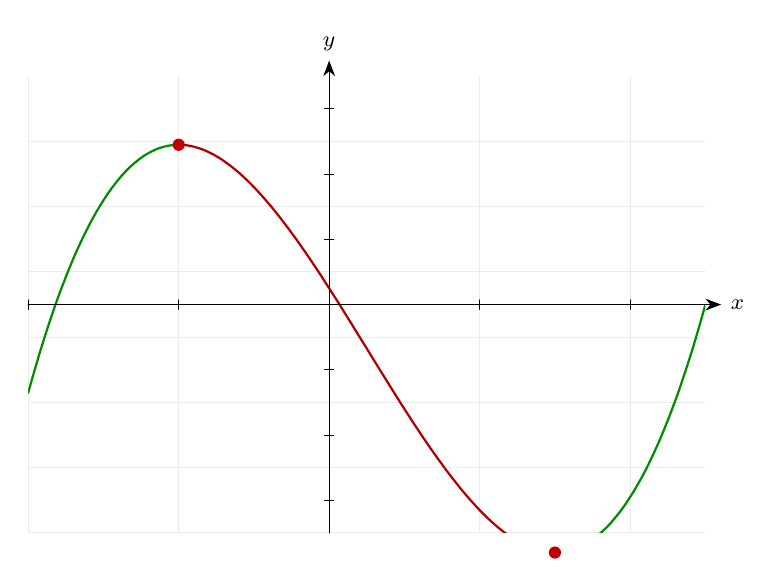
\begin{tikzpicture}[>={Stealth[length=2mm]},font=\footnotesize,line cap=round,line join=round]
\begin{scope}
\clip (0,0) rectangle (8.6,5.8);
\draw[gray!16] (0,-0.414) grid[xstep=1.911,ystep=0.829] (8.6,5.8);
\draw[green!55!black,thick] (0,1.781) -- (0.048,1.953) -- (0.096,2.118) -- (0.143,2.279) -- (0.191,2.433) -- (0.239,2.583) -- (0.287,2.727) -- (0.334,2.866) -- (0.382,3) -- (0.43,3.128) -- (0.478,3.252) -- (0.526,3.371) -- (0.573,3.485) -- (0.621,3.594) -- (0.669,3.698) -- (0.717,3.797) -- (0.764,3.892) -- (0.812,3.982) -- (0.86,4.068) -- (0.908,4.149) -- (0.956,4.226) -- (1.003,4.298) -- (1.051,4.366) -- (1.099,4.43) -- (1.147,4.49) -- (1.194,4.545) -- (1.242,4.597) -- (1.29,4.645) -- (1.338,4.688) -- (1.386,4.728) -- (1.433,4.764) -- (1.481,4.797) -- (1.529,4.825) -- (1.577,4.85) -- (1.624,4.872) -- (1.672,4.89) -- (1.72,4.904) -- (1.768,4.916) -- (1.816,4.924) -- (1.863,4.928) -- (1.911,4.93);
\draw[red!70!black,thick] (1.911,4.93) -- (1.959,4.928) -- (2.007,4.924) -- (2.054,4.916) -- (2.102,4.906) -- (2.15,4.892) -- (2.198,4.876) -- (2.246,4.857) -- (2.293,4.836) -- (2.341,4.812) -- (2.389,4.785) -- (2.437,4.756) -- (2.484,4.724) -- (2.532,4.69) -- (2.58,4.654) -- (2.628,4.615) -- (2.676,4.575) -- (2.723,4.532) -- (2.771,4.487) -- (2.819,4.44) -- (2.867,4.391) -- (2.914,4.341) -- (2.962,4.288) -- (3.01,4.234) -- (3.058,4.178) -- (3.106,4.121) -- (3.153,4.062) -- (3.201,4.001) -- (3.249,3.939) -- (3.297,3.876) -- (3.344,3.811) -- (3.392,3.746) -- (3.44,3.679) -- (3.488,3.61) -- (3.536,3.541) -- (3.583,3.471) -- (3.631,3.4) -- (3.679,3.328) -- (3.727,3.255) -- (3.774,3.181) -- (3.822,3.107) -- (3.87,3.032) -- (3.918,2.957) -- (3.966,2.881) -- (4.013,2.805) -- (4.061,2.728) -- (4.109,2.651) -- (4.157,2.573) -- (4.204,2.496) -- (4.252,2.418) -- (4.3,2.341) -- (4.348,2.263) -- (4.396,2.185) -- (4.443,2.108) -- (4.491,2.031) -- (4.539,1.954) -- (4.587,1.877) -- (4.634,1.801) -- (4.682,1.725) -- (4.73,1.649) -- (4.778,1.574) -- (4.826,1.5) -- (4.873,1.426) -- (4.921,1.354) -- (4.969,1.282) -- (5.017,1.21) -- (5.064,1.14) -- (5.112,1.071) -- (5.16,1.003) -- (5.208,0.936) -- (5.256,0.87) -- (5.303,0.805) -- (5.351,0.742) -- (5.399,0.68) -- (5.447,0.62) -- (5.494,0.561) -- (5.542,0.503) -- (5.59,0.447) -- (5.638,0.393) -- (5.686,0.341) -- (5.733,0.29) -- (5.781,0.241) -- (5.829,0.194) -- (5.877,0.15) -- (5.924,0.107) -- (5.972,0.066) -- (6.02,0.028) -- (6.068,-0.009) -- (6.116,-0.043) -- (6.163,-0.074) -- (6.211,-0.104) -- (6.259,-0.13) -- (6.307,-0.154) -- (6.354,-0.176) -- (6.402,-0.195) -- (6.45,-0.211) -- (6.498,-0.224) -- (6.546,-0.235) -- (6.593,-0.242) -- (6.641,-0.247) -- (6.689,-0.249);
\draw[green!55!black,thick] (6.689,-0.249) -- (6.737,-0.247) -- (6.784,-0.242) -- (6.832,-0.234) -- (6.88,-0.223) -- (6.928,-0.208) -- (6.976,-0.19) -- (7.023,-0.169) -- (7.071,-0.144) -- (7.119,-0.115) -- (7.167,-0.083) -- (7.214,-0.047) -- (7.262,-0.007) -- (7.31,0.037) -- (7.358,0.084) -- (7.406,0.136) -- (7.453,0.192) -- (7.501,0.251) -- (7.549,0.315) -- (7.597,0.383) -- (7.644,0.456) -- (7.692,0.532) -- (7.74,0.614) -- (7.788,0.699) -- (7.836,0.789) -- (7.883,0.884) -- (7.931,0.984) -- (7.979,1.088) -- (8.027,1.197) -- (8.074,1.311) -- (8.122,1.429) -- (8.17,1.553) -- (8.218,1.682) -- (8.266,1.815) -- (8.313,1.954) -- (8.361,2.099) -- (8.409,2.248) -- (8.457,2.403) -- (8.504,2.563) -- (8.552,2.729) -- (8.6,2.9);
\end{scope}
\draw[->] (0,2.9) -- (8.8,2.9) node[right]{$x$};
\draw[->] (3.822,0) -- (3.822,6) node[above]{$y$};
\draw (0,2.84) -- (0,2.96);
\draw (1.911,2.84) -- (1.911,2.96);
\draw (5.733,2.84) -- (5.733,2.96);
\draw (7.644,2.84) -- (7.644,2.96);
\draw (3.762,0.414) -- (3.882,0.414);
\draw (3.762,1.243) -- (3.882,1.243);
\draw (3.762,2.071) -- (3.882,2.071);
\draw (3.762,3.729) -- (3.882,3.729);
\draw (3.762,4.557) -- (3.882,4.557);
\draw (3.762,5.386) -- (3.882,5.386);
\fill[red!75!black] (1.911,4.93) circle (2.2pt);
\fill[red!75!black] (6.689,-0.249) circle (2.2pt);
\end{tikzpicture}
}
\end{center}
\small Curve coloured green where increasing, red where decreasing.\normalsize

\medskip\hrule

\section*{Derivatives and Graphs 14\quad\small\texttt{(d4-014)}}
\addcontentsline{toc}{section}{Derivatives and Graphs 14 (d4-014)}
\textit{Difficulty: Foundation \quad\textbar\quad Marks: 4}

\question{Use differentiation to explain why \( f(x) = x^3 + 3x^2 + 3x + 5 \) is an increasing function for all real values of \( x \).}

\textbf{Worked solution.}

\textit{Step 1: Differentiate.}
\[\begin{gathered}
f'(x) = 3x^2 + 6x + 3
\end{gathered}\]
Power rule.

\textit{Step 2: Factorise the derivative.}
\[\begin{gathered}
f'(x) = 3(x^2 + 2x + 1) = 3(x + 1)^2
\end{gathered}\]
Recognise the perfect square.

\textit{Step 3: Conclude.}
\[\begin{gathered}
f'(x) = 3(x+1)^2 \geq 0 \text{ for all real } x
\end{gathered}\]
A square is always \( \geq 0 \), and equality holds only at \( x = -1 \). Since the gradient is never negative, the function is non-decreasing (and strictly increasing except at the point of inflection \( x = -1 \)).

\begin{answerbox}
\textbf{Final answer:}\quad \(\displaystyle  f'(x) = 3(x+1)^2 \geq 0 \) for all real \(\displaystyle  x \), so \(\displaystyle  f \) is increasing for all real values.
\end{answerbox}
\textbf{Diagram.}

\begin{center}
\resizebox{\ifdim\width>\linewidth \linewidth\else \width\fi}{!}{%
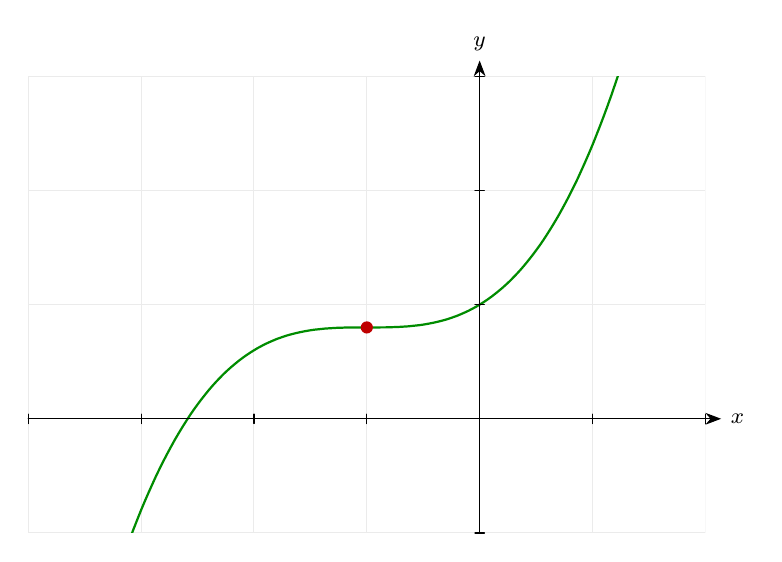
\begin{tikzpicture}[>={Stealth[length=2mm]},font=\footnotesize,line cap=round,line join=round]
\begin{scope}
\clip (0,0) rectangle (8.6,5.8);
\draw[gray!16] (0,0) grid[xstep=1.433,ystep=1.45] (8.6,5.8);
\draw[green!55!black,thick] (0,-5.22) -- (0.048,-4.962) -- (0.096,-4.71) -- (0.143,-4.463) -- (0.191,-4.222) -- (0.239,-3.986) -- (0.287,-3.756) -- (0.334,-3.531) -- (0.382,-3.312) -- (0.43,-3.098) -- (0.478,-2.889) -- (0.526,-2.686) -- (0.573,-2.487) -- (0.621,-2.294) -- (0.669,-2.105) -- (0.717,-1.921) -- (0.764,-1.742) -- (0.812,-1.568) -- (0.86,-1.399) -- (0.908,-1.234) -- (0.956,-1.074) -- (1.003,-0.918) -- (1.051,-0.767) -- (1.099,-0.62) -- (1.147,-0.478) -- (1.194,-0.34) -- (1.242,-0.206) -- (1.29,-0.076) -- (1.338,0.05) -- (1.386,0.172) -- (1.433,0.29) -- (1.481,0.404) -- (1.529,0.514) -- (1.577,0.621) -- (1.624,0.724) -- (1.672,0.823) -- (1.72,0.919) -- (1.768,1.011) -- (1.816,1.1) -- (1.863,1.185) -- (1.911,1.267) -- (1.959,1.346) -- (2.007,1.422) -- (2.054,1.495) -- (2.102,1.565) -- (2.15,1.631) -- (2.198,1.695) -- (2.246,1.756) -- (2.293,1.814) -- (2.341,1.87) -- (2.389,1.923) -- (2.437,1.973) -- (2.484,2.021) -- (2.532,2.066) -- (2.58,2.109) -- (2.628,2.149) -- (2.676,2.188) -- (2.723,2.224) -- (2.771,2.258) -- (2.819,2.29) -- (2.867,2.32) -- (2.914,2.348) -- (2.962,2.374) -- (3.01,2.399) -- (3.058,2.421) -- (3.106,2.442) -- (3.153,2.462) -- (3.201,2.479) -- (3.249,2.496) -- (3.297,2.511) -- (3.344,2.524) -- (3.392,2.536) -- (3.44,2.547) -- (3.488,2.557) -- (3.536,2.566) -- (3.583,2.574) -- (3.631,2.581) -- (3.679,2.586) -- (3.727,2.591) -- (3.774,2.596) -- (3.822,2.599) -- (3.87,2.602) -- (3.918,2.605) -- (3.966,2.606) -- (4.013,2.608) -- (4.061,2.609) -- (4.109,2.609) -- (4.157,2.61) -- (4.204,2.61) -- (4.252,2.61) -- (4.3,2.61);
\draw[green!55!black,thick] (4.3,2.61) -- (4.348,2.61) -- (4.396,2.61) -- (4.443,2.61) -- (4.491,2.611) -- (4.539,2.611) -- (4.587,2.612) -- (4.634,2.614) -- (4.682,2.615) -- (4.73,2.618) -- (4.778,2.621) -- (4.826,2.624) -- (4.873,2.629) -- (4.921,2.634) -- (4.969,2.639) -- (5.017,2.646) -- (5.064,2.654) -- (5.112,2.663) -- (5.16,2.673) -- (5.208,2.684) -- (5.256,2.696) -- (5.303,2.709) -- (5.351,2.724) -- (5.399,2.741) -- (5.447,2.758) -- (5.494,2.778) -- (5.542,2.799) -- (5.59,2.821) -- (5.638,2.846) -- (5.686,2.872) -- (5.733,2.9) -- (5.781,2.93) -- (5.829,2.962) -- (5.877,2.996) -- (5.924,3.032) -- (5.972,3.071) -- (6.02,3.111) -- (6.068,3.154) -- (6.116,3.199) -- (6.163,3.247) -- (6.211,3.297) -- (6.259,3.35) -- (6.307,3.406) -- (6.354,3.464) -- (6.402,3.525) -- (6.45,3.589) -- (6.498,3.655) -- (6.546,3.725) -- (6.593,3.798) -- (6.641,3.874) -- (6.689,3.953) -- (6.737,4.035) -- (6.784,4.12) -- (6.832,4.209) -- (6.88,4.301) -- (6.928,4.397) -- (6.976,4.496) -- (7.023,4.599) -- (7.071,4.706) -- (7.119,4.816) -- (7.167,4.93) -- (7.214,5.048) -- (7.262,5.17) -- (7.31,5.296) -- (7.358,5.426) -- (7.406,5.56) -- (7.453,5.698) -- (7.501,5.84) -- (7.549,5.987) -- (7.597,6.138) -- (7.644,6.294) -- (7.692,6.454) -- (7.74,6.619) -- (7.788,6.788) -- (7.836,6.962) -- (7.883,7.141) -- (7.931,7.325) -- (7.979,7.514) -- (8.027,7.707) -- (8.074,7.906) -- (8.122,8.109) -- (8.17,8.318) -- (8.218,8.532) -- (8.266,8.751) -- (8.313,8.976) -- (8.361,9.206) -- (8.409,9.442) -- (8.457,9.683) -- (8.504,9.93) -- (8.552,10.182) -- (8.6,10.44);
\end{scope}
\draw[->] (0,1.45) -- (8.8,1.45) node[right]{$x$};
\draw[->] (5.733,0) -- (5.733,6) node[above]{$y$};
\draw (0,1.39) -- (0,1.51);
\draw (1.433,1.39) -- (1.433,1.51);
\draw (2.867,1.39) -- (2.867,1.51);
\draw (4.3,1.39) -- (4.3,1.51);
\draw (7.167,1.39) -- (7.167,1.51);
\draw (8.6,1.39) -- (8.6,1.51);
\draw (5.673,0) -- (5.793,0);
\draw (5.673,2.9) -- (5.793,2.9);
\draw (5.673,4.35) -- (5.793,4.35);
\draw (5.673,5.8) -- (5.793,5.8);
\fill[red!75!black] (4.3,2.61) circle (2.2pt);
\end{tikzpicture}
}
\end{center}
\small Curve coloured green where increasing, red where decreasing.\normalsize

\medskip\hrule

\section*{Derivatives and Graphs 15\quad\small\texttt{(d4-015)}}
\addcontentsline{toc}{section}{Derivatives and Graphs 15 (d4-015)}
\textit{Difficulty: Foundation \quad\textbar\quad Marks: 4}

\question{Find the range of values of \( x \) for which \( y = x^3 - 12x + 1 \) is decreasing.}

\textbf{Worked solution.}

\textit{Step 1: Differentiate.}
\[\begin{gathered}
\frac{\mathrm{d}y}{\mathrm{d}x} = 3x^2 - 12
\end{gathered}\]
Power rule.

\textit{Step 2: Form the inequality for decreasing.}
\[\begin{gathered}
3x^2 - 12 < 0 \implies x^2 < 4 \implies -2 < x < 2
\end{gathered}\]
Divide by 3, then solve \( x^2 < 4 \).

\begin{answerbox}
\textbf{Final answer:}\quad \(\displaystyle  -2 < x < 2 \)
\end{answerbox}
\textbf{Diagram.}

\begin{center}
\resizebox{\ifdim\width>\linewidth \linewidth\else \width\fi}{!}{%
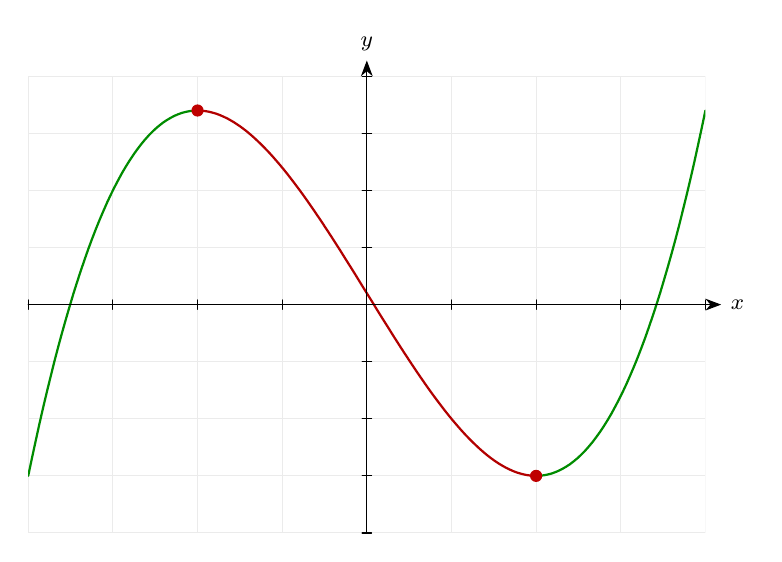
\begin{tikzpicture}[>={Stealth[length=2mm]},font=\footnotesize,line cap=round,line join=round]
\begin{scope}
\clip (0,0) rectangle (8.6,5.8);
\draw[gray!16] (0,0) grid[xstep=1.075,ystep=0.725] (8.6,5.8);
\draw[green!55!black,thick] (0,0.725) -- (0.048,0.954) -- (0.096,1.175) -- (0.143,1.39) -- (0.191,1.599) -- (0.239,1.801) -- (0.287,1.996) -- (0.334,2.185) -- (0.382,2.368) -- (0.43,2.544) -- (0.478,2.714) -- (0.526,2.878) -- (0.573,3.036) -- (0.621,3.188) -- (0.669,3.334) -- (0.717,3.475) -- (0.764,3.609) -- (0.812,3.738) -- (0.86,3.862) -- (0.908,3.98) -- (0.956,4.092) -- (1.003,4.199) -- (1.051,4.301) -- (1.099,4.398) -- (1.147,4.489) -- (1.194,4.576) -- (1.242,4.657) -- (1.29,4.734) -- (1.338,4.806) -- (1.386,4.873) -- (1.433,4.935) -- (1.481,4.993) -- (1.529,5.047) -- (1.577,5.096) -- (1.624,5.14) -- (1.672,5.18) -- (1.72,5.217) -- (1.768,5.248) -- (1.816,5.276) -- (1.863,5.3) -- (1.911,5.32) -- (1.959,5.337) -- (2.007,5.349) -- (2.054,5.358) -- (2.102,5.363) -- (2.15,5.365);
\draw[red!70!black,thick] (2.15,5.365) -- (2.198,5.363) -- (2.246,5.358) -- (2.293,5.35) -- (2.341,5.338) -- (2.389,5.324) -- (2.437,5.306) -- (2.484,5.285) -- (2.532,5.262) -- (2.58,5.235) -- (2.628,5.206) -- (2.676,5.174) -- (2.723,5.14) -- (2.771,5.103) -- (2.819,5.063) -- (2.867,5.021) -- (2.914,4.977) -- (2.962,4.931) -- (3.01,4.882) -- (3.058,4.832) -- (3.106,4.779) -- (3.153,4.725) -- (3.201,4.669) -- (3.249,4.611) -- (3.297,4.551) -- (3.344,4.49) -- (3.392,4.427) -- (3.44,4.363) -- (3.488,4.297) -- (3.536,4.23) -- (3.583,4.162) -- (3.631,4.093) -- (3.679,4.022) -- (3.727,3.951) -- (3.774,3.879) -- (3.822,3.806) -- (3.87,3.732) -- (3.918,3.657) -- (3.966,3.582) -- (4.013,3.506) -- (4.061,3.43) -- (4.109,3.354) -- (4.157,3.277) -- (4.204,3.2) -- (4.252,3.122) -- (4.3,3.045) -- (4.348,2.968) -- (4.396,2.89) -- (4.443,2.813) -- (4.491,2.736) -- (4.539,2.66) -- (4.587,2.584) -- (4.634,2.508) -- (4.682,2.433) -- (4.73,2.358) -- (4.778,2.284) -- (4.826,2.211) -- (4.873,2.139) -- (4.921,2.068) -- (4.969,1.997) -- (5.017,1.928) -- (5.064,1.86) -- (5.112,1.793) -- (5.16,1.727) -- (5.208,1.663) -- (5.256,1.6) -- (5.303,1.539) -- (5.351,1.479) -- (5.399,1.421) -- (5.447,1.365) -- (5.494,1.311) -- (5.542,1.258) -- (5.59,1.208) -- (5.638,1.159) -- (5.686,1.113) -- (5.733,1.069) -- (5.781,1.027) -- (5.829,0.987) -- (5.877,0.95) -- (5.924,0.916) -- (5.972,0.884) -- (6.02,0.855) -- (6.068,0.828) -- (6.116,0.805) -- (6.163,0.784) -- (6.211,0.766) -- (6.259,0.752) -- (6.307,0.74) -- (6.354,0.732) -- (6.402,0.727) -- (6.45,0.725);
\draw[green!55!black,thick] (6.45,0.725) -- (6.498,0.727) -- (6.546,0.732) -- (6.593,0.741) -- (6.641,0.753) -- (6.689,0.77) -- (6.737,0.79) -- (6.784,0.814) -- (6.832,0.842) -- (6.88,0.873) -- (6.928,0.91) -- (6.976,0.95) -- (7.023,0.994) -- (7.071,1.043) -- (7.119,1.097) -- (7.167,1.155) -- (7.214,1.217) -- (7.262,1.284) -- (7.31,1.356) -- (7.358,1.433) -- (7.406,1.514) -- (7.453,1.601) -- (7.501,1.692) -- (7.549,1.789) -- (7.597,1.891) -- (7.644,1.998) -- (7.692,2.11) -- (7.74,2.228) -- (7.788,2.352) -- (7.836,2.481) -- (7.883,2.615) -- (7.931,2.756) -- (7.979,2.902) -- (8.027,3.054) -- (8.074,3.212) -- (8.122,3.376) -- (8.17,3.546) -- (8.218,3.722) -- (8.266,3.905) -- (8.313,4.094) -- (8.361,4.289) -- (8.409,4.491) -- (8.457,4.7) -- (8.504,4.915) -- (8.552,5.136) -- (8.6,5.365);
\end{scope}
\draw[->] (0,2.9) -- (8.8,2.9) node[right]{$x$};
\draw[->] (4.3,0) -- (4.3,6) node[above]{$y$};
\draw (0,2.84) -- (0,2.96);
\draw (1.075,2.84) -- (1.075,2.96);
\draw (2.15,2.84) -- (2.15,2.96);
\draw (3.225,2.84) -- (3.225,2.96);
\draw (5.375,2.84) -- (5.375,2.96);
\draw (6.45,2.84) -- (6.45,2.96);
\draw (7.525,2.84) -- (7.525,2.96);
\draw (8.6,2.84) -- (8.6,2.96);
\draw (4.24,0) -- (4.36,0);
\draw (4.24,0.725) -- (4.36,0.725);
\draw (4.24,1.45) -- (4.36,1.45);
\draw (4.24,2.175) -- (4.36,2.175);
\draw (4.24,3.625) -- (4.36,3.625);
\draw (4.24,4.35) -- (4.36,4.35);
\draw (4.24,5.075) -- (4.36,5.075);
\draw (4.24,5.8) -- (4.36,5.8);
\fill[red!75!black] (2.15,5.365) circle (2.2pt);
\fill[red!75!black] (6.45,0.725) circle (2.2pt);
\end{tikzpicture}
}
\end{center}
\small Curve coloured green where increasing, red where decreasing.\normalsize

\medskip\hrule

\section*{Derivatives and Graphs 16\quad\small\texttt{(d4-016)}}
\addcontentsline{toc}{section}{Derivatives and Graphs 16 (d4-016)}
\textit{Difficulty: Foundation \quad\textbar\quad Marks: 3}

\question{The function \( y = 4 + 6x - x^2 \) is decreasing for \( x > k \). Find the value of \( k \).}

\textbf{Worked solution.}

\textit{Step 1: Differentiate.}
\[\begin{gathered}
\frac{\mathrm{d}y}{\mathrm{d}x} = 6 - 2x
\end{gathered}\]
Power rule.

\textit{Step 2: Find where the derivative changes from positive to negative.}
\[\begin{gathered}
6 - 2x = 0 \implies x = 3
\end{gathered}\]
The stationary point is at \( x = 3 \).

\textit{Step 3: The function is decreasing when \( 6 - 2x < 0 \), i.e. \( x > 3 \).}
\[\begin{gathered}
k = 3
\end{gathered}\]
Since the coefficient of \( x^2 \) is negative, this is an inverted parabola: increasing then decreasing.

\begin{answerbox}
\textbf{Final answer:}\quad \(\displaystyle  k = 3 \)
\end{answerbox}
\textbf{Diagram.}

\begin{center}
\resizebox{\ifdim\width>\linewidth \linewidth\else \width\fi}{!}{%
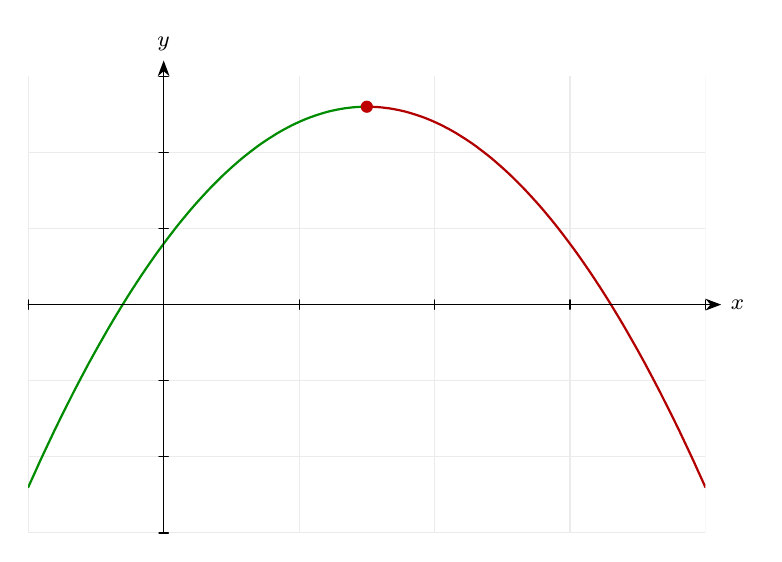
\begin{tikzpicture}[>={Stealth[length=2mm]},font=\footnotesize,line cap=round,line join=round]
\begin{scope}
\clip (0,0) rectangle (8.6,5.8);
\draw[gray!16] (0,0) grid[xstep=1.72,ystep=0.967] (8.6,5.8);
\draw[green!55!black,thick] (0,0.58) -- (0.048,0.687) -- (0.096,0.792) -- (0.143,0.897) -- (0.191,1) -- (0.239,1.102) -- (0.287,1.203) -- (0.334,1.303) -- (0.382,1.401) -- (0.43,1.498) -- (0.478,1.594) -- (0.526,1.689) -- (0.573,1.783) -- (0.621,1.875) -- (0.669,1.967) -- (0.717,2.057) -- (0.764,2.146) -- (0.812,2.233) -- (0.86,2.32) -- (0.908,2.405) -- (0.956,2.489) -- (1.003,2.572) -- (1.051,2.654) -- (1.099,2.735) -- (1.147,2.814) -- (1.194,2.892) -- (1.242,2.969) -- (1.29,3.045) -- (1.338,3.12) -- (1.386,3.193) -- (1.433,3.265) -- (1.481,3.336) -- (1.529,3.406) -- (1.577,3.475) -- (1.624,3.542) -- (1.672,3.608) -- (1.72,3.673) -- (1.768,3.737) -- (1.816,3.8) -- (1.863,3.861) -- (1.911,3.922) -- (1.959,3.981) -- (2.007,4.039) -- (2.054,4.095) -- (2.102,4.151) -- (2.15,4.205) -- (2.198,4.258) -- (2.246,4.31) -- (2.293,4.361) -- (2.341,4.41) -- (2.389,4.459) -- (2.437,4.506) -- (2.484,4.552) -- (2.532,4.596) -- (2.58,4.64) -- (2.628,4.682) -- (2.676,4.724) -- (2.723,4.764) -- (2.771,4.802) -- (2.819,4.84) -- (2.867,4.876) -- (2.914,4.912) -- (2.962,4.946) -- (3.01,4.978) -- (3.058,5.01) -- (3.106,5.04) -- (3.153,5.07) -- (3.201,5.098) -- (3.249,5.125) -- (3.297,5.15) -- (3.344,5.175) -- (3.392,5.198) -- (3.44,5.22) -- (3.488,5.241) -- (3.536,5.261) -- (3.583,5.279) -- (3.631,5.296) -- (3.679,5.312) -- (3.727,5.327) -- (3.774,5.341) -- (3.822,5.354) -- (3.87,5.365) -- (3.918,5.375) -- (3.966,5.384) -- (4.013,5.392) -- (4.061,5.398) -- (4.109,5.404) -- (4.157,5.408) -- (4.204,5.411) -- (4.252,5.413) -- (4.3,5.413);
\draw[red!70!black,thick] (4.3,5.413) -- (4.348,5.413) -- (4.396,5.411) -- (4.443,5.408) -- (4.491,5.404) -- (4.539,5.398) -- (4.587,5.392) -- (4.634,5.384) -- (4.682,5.375) -- (4.73,5.365) -- (4.778,5.354) -- (4.826,5.341) -- (4.873,5.327) -- (4.921,5.312) -- (4.969,5.296) -- (5.017,5.279) -- (5.064,5.261) -- (5.112,5.241) -- (5.16,5.22) -- (5.208,5.198) -- (5.256,5.175) -- (5.303,5.15) -- (5.351,5.125) -- (5.399,5.098) -- (5.447,5.07) -- (5.494,5.04) -- (5.542,5.01) -- (5.59,4.978) -- (5.638,4.946) -- (5.686,4.912) -- (5.733,4.876) -- (5.781,4.84) -- (5.829,4.802) -- (5.877,4.764) -- (5.924,4.724) -- (5.972,4.682) -- (6.02,4.64) -- (6.068,4.596) -- (6.116,4.552) -- (6.163,4.506) -- (6.211,4.459) -- (6.259,4.41) -- (6.307,4.361) -- (6.354,4.31) -- (6.402,4.258) -- (6.45,4.205) -- (6.498,4.151) -- (6.546,4.095) -- (6.593,4.039) -- (6.641,3.981) -- (6.689,3.922) -- (6.737,3.861) -- (6.784,3.8) -- (6.832,3.737) -- (6.88,3.673) -- (6.928,3.608) -- (6.976,3.542) -- (7.023,3.475) -- (7.071,3.406) -- (7.119,3.336) -- (7.167,3.265) -- (7.214,3.193) -- (7.262,3.12) -- (7.31,3.045) -- (7.358,2.969) -- (7.406,2.892) -- (7.453,2.814) -- (7.501,2.735) -- (7.549,2.654) -- (7.597,2.572) -- (7.644,2.489) -- (7.692,2.405) -- (7.74,2.32) -- (7.788,2.233) -- (7.836,2.146) -- (7.883,2.057) -- (7.931,1.967) -- (7.979,1.875) -- (8.027,1.783) -- (8.074,1.689) -- (8.122,1.594) -- (8.17,1.498) -- (8.218,1.401) -- (8.266,1.303) -- (8.313,1.203) -- (8.361,1.102) -- (8.409,1) -- (8.457,0.897) -- (8.504,0.792) -- (8.552,0.687) -- (8.6,0.58);
\end{scope}
\draw[->] (0,2.9) -- (8.8,2.9) node[right]{$x$};
\draw[->] (1.72,0) -- (1.72,6) node[above]{$y$};
\draw (0,2.84) -- (0,2.96);
\draw (3.44,2.84) -- (3.44,2.96);
\draw (5.16,2.84) -- (5.16,2.96);
\draw (6.88,2.84) -- (6.88,2.96);
\draw (8.6,2.84) -- (8.6,2.96);
\draw (1.66,0) -- (1.78,0);
\draw (1.66,0.967) -- (1.78,0.967);
\draw (1.66,1.933) -- (1.78,1.933);
\draw (1.66,3.867) -- (1.78,3.867);
\draw (1.66,4.833) -- (1.78,4.833);
\draw (1.66,5.8) -- (1.78,5.8);
\fill[red!75!black] (4.3,5.413) circle (2.2pt);
\end{tikzpicture}
}
\end{center}
\small Curve coloured green where increasing, red where decreasing.\normalsize

\medskip\hrule

\section*{Derivatives and Graphs 17\quad\small\texttt{(d4-017)}}
\addcontentsline{toc}{section}{Derivatives and Graphs 17 (d4-017)}
\textit{Difficulty: Foundation \quad\textbar\quad Marks: 4}

\question{Find the range of values of \( x \) for which \( f(x) = x^3 - 6x^2 + 15x - 7 \) is increasing.}

\textbf{Worked solution.}

\textit{Step 1: Differentiate.}
\[\begin{gathered}
f'(x) = 3x^2 - 12x + 15
\end{gathered}\]
Power rule.

\textit{Step 2: Check the discriminant of \( f'(x) \).}
\[\begin{gathered}
\Delta = (-12)^2 - 4(3)(15) = 144 - 180 = -36 < 0
\end{gathered}\]
Since \( \Delta < 0 \) and the leading coefficient is positive, \( f'(x) > 0 \) for all \( x \).

\textit{Step 3: Conclude.}
\[\begin{gathered}
f'(x) = 3x^2 - 12x + 15 > 0 \text{ for all real } x
\end{gathered}\]
The function is increasing for all real values of \( x \).

\begin{answerbox}
\textbf{Final answer:}\quad \(\displaystyle  f(x) \) is increasing for all real values of \(\displaystyle  x \).
\end{answerbox}
\textbf{Diagram.}

\begin{center}
\resizebox{\ifdim\width>\linewidth \linewidth\else \width\fi}{!}{%
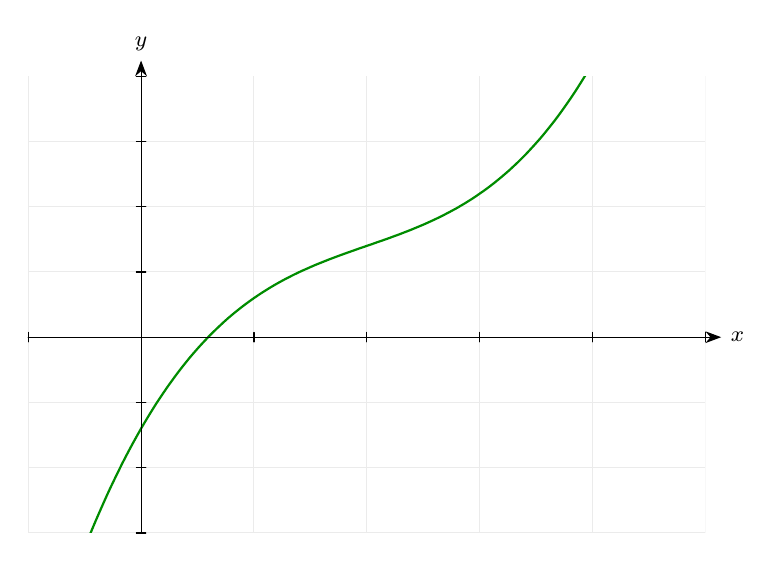
\begin{tikzpicture}[>={Stealth[length=2mm]},font=\footnotesize,line cap=round,line join=round]
\begin{scope}
\clip (0,0) rectangle (8.6,5.8);
\draw[gray!16] (0,0) grid[xstep=1.433,ystep=0.829] (8.6,5.8);
\draw[green!55!black,thick] (0,-2.32) -- (0.048,-2.156) -- (0.096,-1.995) -- (0.143,-1.838) -- (0.191,-1.683) -- (0.239,-1.532) -- (0.287,-1.384) -- (0.334,-1.239) -- (0.382,-1.097) -- (0.43,-0.958) -- (0.478,-0.822) -- (0.526,-0.689) -- (0.573,-0.559) -- (0.621,-0.432) -- (0.669,-0.308) -- (0.717,-0.186) -- (0.764,-0.068) -- (0.812,0.048) -- (0.86,0.162) -- (0.908,0.272) -- (0.956,0.381) -- (1.003,0.486) -- (1.051,0.589) -- (1.099,0.689) -- (1.147,0.787) -- (1.194,0.883) -- (1.242,0.976) -- (1.29,1.067) -- (1.338,1.156) -- (1.386,1.242) -- (1.433,1.326) -- (1.481,1.407) -- (1.529,1.487) -- (1.577,1.565) -- (1.624,1.64) -- (1.672,1.713) -- (1.72,1.784) -- (1.768,1.854) -- (1.816,1.921) -- (1.863,1.986) -- (1.911,2.05) -- (1.959,2.112) -- (2.007,2.172) -- (2.054,2.23) -- (2.102,2.286) -- (2.15,2.341) -- (2.198,2.394) -- (2.246,2.445) -- (2.293,2.495) -- (2.341,2.543) -- (2.389,2.59) -- (2.437,2.635) -- (2.484,2.679) -- (2.532,2.722) -- (2.58,2.763) -- (2.628,2.803) -- (2.676,2.841) -- (2.723,2.878) -- (2.771,2.914) -- (2.819,2.949) -- (2.867,2.983) -- (2.914,3.015) -- (2.962,3.047) -- (3.01,3.077) -- (3.058,3.107) -- (3.106,3.136) -- (3.153,3.163) -- (3.201,3.19) -- (3.249,3.216) -- (3.297,3.241) -- (3.344,3.265) -- (3.392,3.289) -- (3.44,3.312) -- (3.488,3.334) -- (3.536,3.355) -- (3.583,3.376) -- (3.631,3.397) -- (3.679,3.417) -- (3.727,3.436) -- (3.774,3.455) -- (3.822,3.474) -- (3.87,3.492) -- (3.918,3.51) -- (3.966,3.528) -- (4.013,3.545) -- (4.061,3.562) -- (4.109,3.579) -- (4.157,3.596) -- (4.204,3.613) -- (4.252,3.629) -- (4.3,3.646) -- (4.348,3.662) -- (4.396,3.679) -- (4.443,3.696) -- (4.491,3.712) -- (4.539,3.729) -- (4.587,3.746) -- (4.634,3.764) -- (4.682,3.781) -- (4.73,3.799) -- (4.778,3.818) -- (4.826,3.836) -- (4.873,3.855) -- (4.921,3.875) -- (4.969,3.895) -- (5.017,3.915) -- (5.064,3.936) -- (5.112,3.958) -- (5.16,3.98) -- (5.208,4.003) -- (5.256,4.026) -- (5.303,4.051) -- (5.351,4.076) -- (5.399,4.102) -- (5.447,4.128) -- (5.494,4.156) -- (5.542,4.184) -- (5.59,4.214) -- (5.638,4.244) -- (5.686,4.276) -- (5.733,4.309) -- (5.781,4.342) -- (5.829,4.377) -- (5.877,4.413) -- (5.924,4.45) -- (5.972,4.489) -- (6.02,4.529) -- (6.068,4.57) -- (6.116,4.612) -- (6.163,4.656) -- (6.211,4.701) -- (6.259,4.748) -- (6.307,4.796) -- (6.354,4.846) -- (6.402,4.898) -- (6.45,4.951) -- (6.498,5.005) -- (6.546,5.062) -- (6.593,5.12) -- (6.641,5.18) -- (6.689,5.241) -- (6.737,5.305) -- (6.784,5.37) -- (6.832,5.438) -- (6.88,5.507) -- (6.928,5.578) -- (6.976,5.652) -- (7.023,5.727) -- (7.071,5.804) -- (7.119,5.884) -- (7.167,5.966) -- (7.214,6.05) -- (7.262,6.136) -- (7.31,6.224) -- (7.358,6.315) -- (7.406,6.408) -- (7.453,6.504) -- (7.501,6.602) -- (7.549,6.702) -- (7.597,6.805) -- (7.644,6.911) -- (7.692,7.019) -- (7.74,7.13) -- (7.788,7.243) -- (7.836,7.359) -- (7.883,7.478) -- (7.931,7.599) -- (7.979,7.724) -- (8.027,7.851) -- (8.074,7.981) -- (8.122,8.114) -- (8.17,8.25) -- (8.218,8.389) -- (8.266,8.531) -- (8.313,8.675) -- (8.361,8.824) -- (8.409,8.975) -- (8.457,9.129) -- (8.504,9.287) -- (8.552,9.447) -- (8.6,9.611);
\end{scope}
\draw[->] (0,2.486) -- (8.8,2.486) node[right]{$x$};
\draw[->] (1.433,0) -- (1.433,6) node[above]{$y$};
\draw (0,2.426) -- (0,2.546);
\draw (2.867,2.426) -- (2.867,2.546);
\draw (4.3,2.426) -- (4.3,2.546);
\draw (5.733,2.426) -- (5.733,2.546);
\draw (7.167,2.426) -- (7.167,2.546);
\draw (8.6,2.426) -- (8.6,2.546);
\draw (1.373,0) -- (1.493,0);
\draw (1.373,0.829) -- (1.493,0.829);
\draw (1.373,1.657) -- (1.493,1.657);
\draw (1.373,3.314) -- (1.493,3.314);
\draw (1.373,4.143) -- (1.493,4.143);
\draw (1.373,4.971) -- (1.493,4.971);
\draw (1.373,5.8) -- (1.493,5.8);
\end{tikzpicture}
}
\end{center}
\small Curve coloured green where increasing, red where decreasing.\normalsize

\medskip\hrule

\section*{Derivatives and Graphs 18\quad\small\texttt{(d4-018)}}
\addcontentsline{toc}{section}{Derivatives and Graphs 18 (d4-018)}
\textit{Difficulty: Foundation \quad\textbar\quad Marks: 3}

\question{Given that \( g(x) = 3 - 4x - 2x^2 \) is a decreasing function for \( x > k \), find \( k \).}

\textbf{Worked solution.}

\textit{Step 1: Differentiate.}
\[\begin{gathered}
g'(x) = -4 - 4x
\end{gathered}\]
Power rule.

\textit{Step 2: Find where \( g'(x) = 0 \).}
\[\begin{gathered}
-4 - 4x = 0 \implies x = -1
\end{gathered}\]
This is the stationary point of \( g \).

\textit{Step 3: Check when the gradient is negative.}
\[\begin{gathered}
-4 - 4x < 0 \implies x > -1
\end{gathered}\]
The inverted parabola decreases for \( x > -1 \).

\begin{answerbox}
\textbf{Final answer:}\quad \(\displaystyle  k = -1 \)
\end{answerbox}
\textbf{Diagram.}

\begin{center}
\resizebox{\ifdim\width>\linewidth \linewidth\else \width\fi}{!}{%
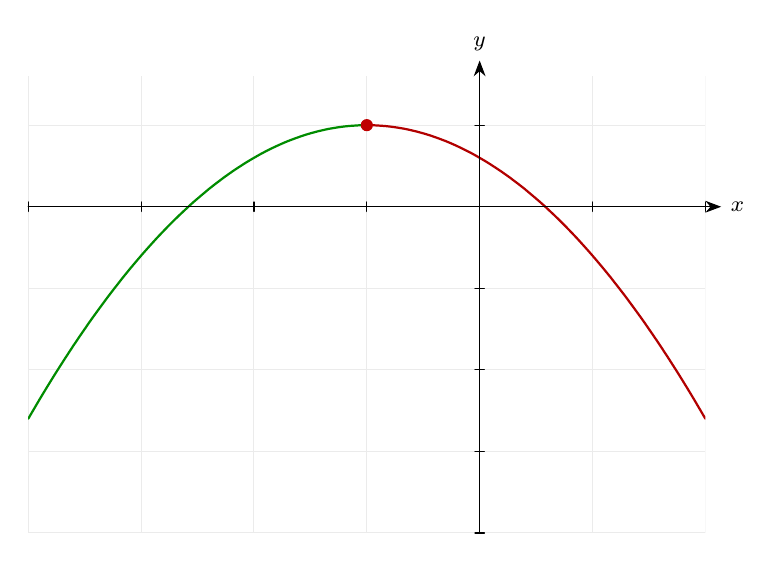
\begin{tikzpicture}[>={Stealth[length=2mm]},font=\footnotesize,line cap=round,line join=round]
\begin{scope}
\clip (0,0) rectangle (8.6,5.8);
\draw[gray!16] (0,0) grid[xstep=1.433,ystep=1.036] (8.6,5.8);
\draw[green!55!black,thick] (0,1.45) -- (0.048,1.532) -- (0.096,1.614) -- (0.143,1.694) -- (0.191,1.774) -- (0.239,1.853) -- (0.287,1.931) -- (0.334,2.007) -- (0.382,2.083) -- (0.43,2.158) -- (0.478,2.233) -- (0.526,2.306) -- (0.573,2.378) -- (0.621,2.449) -- (0.669,2.52) -- (0.717,2.589) -- (0.764,2.658) -- (0.812,2.726) -- (0.86,2.792) -- (0.908,2.858) -- (0.956,2.923) -- (1.003,2.987) -- (1.051,3.05) -- (1.099,3.112) -- (1.147,3.173) -- (1.194,3.234) -- (1.242,3.293) -- (1.29,3.352) -- (1.338,3.409) -- (1.386,3.466) -- (1.433,3.521) -- (1.481,3.576) -- (1.529,3.63) -- (1.577,3.683) -- (1.624,3.735) -- (1.672,3.786) -- (1.72,3.836) -- (1.768,3.886) -- (1.816,3.934) -- (1.863,3.981) -- (1.911,4.028) -- (1.959,4.073) -- (2.007,4.118) -- (2.054,4.162) -- (2.102,4.205) -- (2.15,4.246) -- (2.198,4.287) -- (2.246,4.327) -- (2.293,4.367) -- (2.341,4.405) -- (2.389,4.442) -- (2.437,4.478) -- (2.484,4.514) -- (2.532,4.548) -- (2.58,4.582) -- (2.628,4.615) -- (2.676,4.646) -- (2.723,4.677) -- (2.771,4.707) -- (2.819,4.736) -- (2.867,4.764) -- (2.914,4.791) -- (2.962,4.818) -- (3.01,4.843) -- (3.058,4.867) -- (3.106,4.891) -- (3.153,4.913) -- (3.201,4.935) -- (3.249,4.956) -- (3.297,4.976) -- (3.344,4.994) -- (3.392,5.012) -- (3.44,5.029) -- (3.488,5.046) -- (3.536,5.061) -- (3.583,5.075) -- (3.631,5.088) -- (3.679,5.101) -- (3.727,5.112) -- (3.774,5.123) -- (3.822,5.133) -- (3.87,5.141) -- (3.918,5.149) -- (3.966,5.156) -- (4.013,5.162) -- (4.061,5.167) -- (4.109,5.171) -- (4.157,5.174) -- (4.204,5.177) -- (4.252,5.178) -- (4.3,5.179);
\draw[red!70!black,thick] (4.3,5.179) -- (4.348,5.178) -- (4.396,5.177) -- (4.443,5.174) -- (4.491,5.171) -- (4.539,5.167) -- (4.587,5.162) -- (4.634,5.156) -- (4.682,5.149) -- (4.73,5.141) -- (4.778,5.133) -- (4.826,5.123) -- (4.873,5.112) -- (4.921,5.101) -- (4.969,5.088) -- (5.017,5.075) -- (5.064,5.061) -- (5.112,5.046) -- (5.16,5.029) -- (5.208,5.012) -- (5.256,4.994) -- (5.303,4.976) -- (5.351,4.956) -- (5.399,4.935) -- (5.447,4.913) -- (5.494,4.891) -- (5.542,4.867) -- (5.59,4.843) -- (5.638,4.818) -- (5.686,4.791) -- (5.733,4.764) -- (5.781,4.736) -- (5.829,4.707) -- (5.877,4.677) -- (5.924,4.646) -- (5.972,4.615) -- (6.02,4.582) -- (6.068,4.548) -- (6.116,4.514) -- (6.163,4.478) -- (6.211,4.442) -- (6.259,4.405) -- (6.307,4.367) -- (6.354,4.327) -- (6.402,4.287) -- (6.45,4.246) -- (6.498,4.205) -- (6.546,4.162) -- (6.593,4.118) -- (6.641,4.073) -- (6.689,4.028) -- (6.737,3.981) -- (6.784,3.934) -- (6.832,3.886) -- (6.88,3.836) -- (6.928,3.786) -- (6.976,3.735) -- (7.023,3.683) -- (7.071,3.63) -- (7.119,3.576) -- (7.167,3.521) -- (7.214,3.466) -- (7.262,3.409) -- (7.31,3.352) -- (7.358,3.293) -- (7.406,3.234) -- (7.453,3.173) -- (7.501,3.112) -- (7.549,3.05) -- (7.597,2.987) -- (7.644,2.923) -- (7.692,2.858) -- (7.74,2.792) -- (7.788,2.726) -- (7.836,2.658) -- (7.883,2.589) -- (7.931,2.52) -- (7.979,2.449) -- (8.027,2.378) -- (8.074,2.306) -- (8.122,2.233) -- (8.17,2.158) -- (8.218,2.083) -- (8.266,2.007) -- (8.313,1.931) -- (8.361,1.853) -- (8.409,1.774) -- (8.457,1.694) -- (8.504,1.614) -- (8.552,1.532) -- (8.6,1.45);
\end{scope}
\draw[->] (0,4.143) -- (8.8,4.143) node[right]{$x$};
\draw[->] (5.733,0) -- (5.733,6) node[above]{$y$};
\draw (0,4.083) -- (0,4.203);
\draw (1.433,4.083) -- (1.433,4.203);
\draw (2.867,4.083) -- (2.867,4.203);
\draw (4.3,4.083) -- (4.3,4.203);
\draw (7.167,4.083) -- (7.167,4.203);
\draw (8.6,4.083) -- (8.6,4.203);
\draw (5.673,0) -- (5.793,0);
\draw (5.673,1.036) -- (5.793,1.036);
\draw (5.673,2.071) -- (5.793,2.071);
\draw (5.673,3.107) -- (5.793,3.107);
\draw (5.673,5.179) -- (5.793,5.179);
\fill[red!75!black] (4.3,5.179) circle (2.2pt);
\end{tikzpicture}
}
\end{center}
\small Curve coloured green where increasing, red where decreasing.\normalsize

\medskip\hrule

\section*{Derivatives and Graphs 19\quad\small\texttt{(d4-019)}}
\addcontentsline{toc}{section}{Derivatives and Graphs 19 (d4-019)}
\textit{Difficulty: Foundation \quad\textbar\quad Marks: 7}

\question{Sketch the curve \( y = x^3 - 3x^2 \), clearly labelling: (i) the coordinates where the curve crosses the axes, (ii) the coordinates of any stationary points, and (iii) the nature of each stationary point.}

\textbf{Worked solution.}

\textit{Step 1: Find \( y \)-intercept (set \( x = 0 \)).}
\[\begin{gathered}
y = 0
\end{gathered}\]
The curve passes through the origin.

\textit{Step 2: Find \( x \)-intercepts (set \( y = 0 \)).}
\[\begin{gathered}
x^3 - 3x^2 = 0 \implies x^2(x - 3) = 0 \implies x = 0 \text{ (double root) and } x = 3
\end{gathered}\]
The double root at \( x = 0 \) means the curve touches but does not cross the axis there.

\textit{Step 3: Find stationary points.}
\[\begin{gathered}
\frac{\mathrm{d}y}{\mathrm{d}x} = 3x^2 - 6x = 3x(x-2) = 0 \implies x = 0 \text{ or } x = 2
\end{gathered}\]
Set \( \dfrac{\mathrm{d}y}{\mathrm{d}x} = 0 \) and factorise.

\textit{Step 4: Find \( y \)-coordinates of stationary points.}
\[\begin{gathered}
x=0: y=0; \quad x=2: y = 8 - 12 = -4
\end{gathered}\]
Substitute into the original equation.

\textit{Step 5: Classify using second derivative.}
\[\begin{gathered}
\frac{\mathrm{d}^2y}{\mathrm{d}x^2} = 6x - 6 \newline x=0: -6 < 0 \Rightarrow \text{maximum} \newline x=2: 6 > 0 \Rightarrow \text{minimum}
\end{gathered}\]
Evaluate \( \dfrac{\mathrm{d}^2y}{\mathrm{d}x^2} \) at each stationary point.

\textit{Step 6: Sketch description.}
\[\begin{gathered}
\text{Cubic with positive leading coefficient; passes through } (0,0),\, (3,0); \text{ local max at } (0,0),\text{ local min at } (2,-4).
\end{gathered}\]
The curve rises from bottom-left to top-right, with a local maximum at the origin and a local minimum at \( (2,-4) \).

\begin{answerbox}
\textbf{Final answer:}\quad Crosses axes at \(\displaystyle  (0, 0) \) and \(\displaystyle  (3, 0) \). Local maximum at \(\displaystyle  (0, 0) \); local minimum at \(\displaystyle  (2, -4) \).
\end{answerbox}
\textbf{Diagram.}

\begin{center}
\resizebox{\ifdim\width>\linewidth \linewidth\else \width\fi}{!}{%
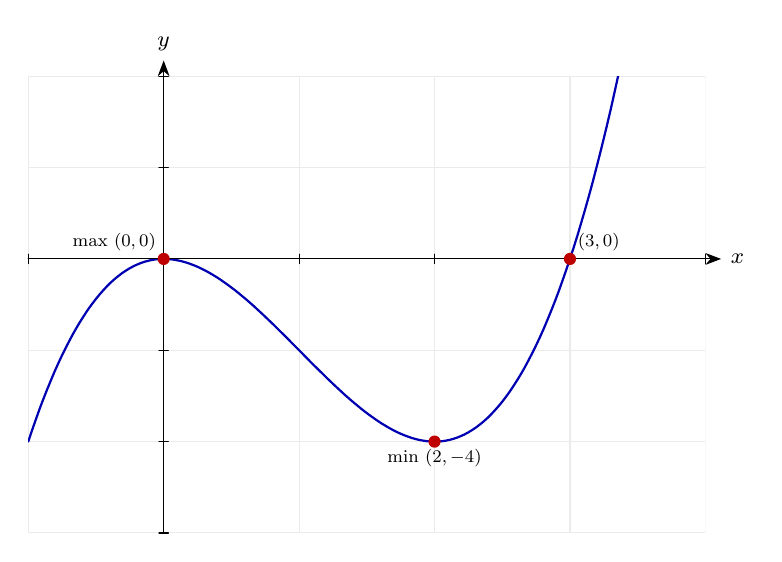
\begin{tikzpicture}[>={Stealth[length=2mm]},font=\footnotesize,line cap=round,line join=round]
\begin{scope}
\clip (0,0) rectangle (8.6,5.8);
\draw[gray!16] (0,0) grid[xstep=1.72,ystep=1.16] (8.6,5.8);
\draw[blue!70!black,thick] (0,1.16) -- (0.048,1.302) -- (0.096,1.439) -- (0.143,1.571) -- (0.191,1.698) -- (0.239,1.819) -- (0.287,1.936) -- (0.334,2.048) -- (0.382,2.155) -- (0.43,2.257) -- (0.478,2.354) -- (0.526,2.447) -- (0.573,2.535) -- (0.621,2.619) -- (0.669,2.698) -- (0.717,2.773) -- (0.764,2.844) -- (0.812,2.91) -- (0.86,2.972) -- (0.908,3.031) -- (0.956,3.085) -- (1.003,3.136) -- (1.051,3.183) -- (1.099,3.226) -- (1.147,3.265) -- (1.194,3.301) -- (1.242,3.333) -- (1.29,3.362) -- (1.338,3.388) -- (1.386,3.41) -- (1.433,3.429) -- (1.481,3.445) -- (1.529,3.458) -- (1.577,3.468) -- (1.624,3.475) -- (1.672,3.479) -- (1.72,3.48) -- (1.768,3.479) -- (1.816,3.475) -- (1.863,3.468) -- (1.911,3.459) -- (1.959,3.448) -- (2.007,3.434) -- (2.054,3.418) -- (2.102,3.4) -- (2.15,3.38) -- (2.198,3.358) -- (2.246,3.334) -- (2.293,3.308) -- (2.341,3.28) -- (2.389,3.251) -- (2.437,3.22) -- (2.484,3.187) -- (2.532,3.153) -- (2.58,3.117) -- (2.628,3.081) -- (2.676,3.042) -- (2.723,3.003) -- (2.771,2.963) -- (2.819,2.921) -- (2.867,2.879) -- (2.914,2.835) -- (2.962,2.791) -- (3.01,2.746) -- (3.058,2.7) -- (3.106,2.654) -- (3.153,2.607) -- (3.201,2.56) -- (3.249,2.513) -- (3.297,2.465) -- (3.344,2.417) -- (3.392,2.368) -- (3.44,2.32) -- (3.488,2.272) -- (3.536,2.223) -- (3.583,2.175) -- (3.631,2.127) -- (3.679,2.08) -- (3.727,2.033) -- (3.774,1.986) -- (3.822,1.94) -- (3.87,1.894) -- (3.918,1.849) -- (3.966,1.805) -- (4.013,1.761) -- (4.061,1.719) -- (4.109,1.677) -- (4.157,1.637) -- (4.204,1.598) -- (4.252,1.559) -- (4.3,1.522) -- (4.348,1.487) -- (4.396,1.453) -- (4.443,1.42) -- (4.491,1.389) -- (4.539,1.36) -- (4.587,1.332) -- (4.634,1.306) -- (4.682,1.282) -- (4.73,1.26) -- (4.778,1.24) -- (4.826,1.222) -- (4.873,1.206) -- (4.921,1.192) -- (4.969,1.181) -- (5.017,1.172) -- (5.064,1.165) -- (5.112,1.161) -- (5.16,1.16) -- (5.208,1.161) -- (5.256,1.165) -- (5.303,1.172) -- (5.351,1.182) -- (5.399,1.195) -- (5.447,1.211) -- (5.494,1.23) -- (5.542,1.252) -- (5.59,1.278) -- (5.638,1.307) -- (5.686,1.339) -- (5.733,1.375) -- (5.781,1.414) -- (5.829,1.457) -- (5.877,1.504) -- (5.924,1.555) -- (5.972,1.609) -- (6.02,1.667) -- (6.068,1.73) -- (6.116,1.796) -- (6.163,1.867) -- (6.211,1.942) -- (6.259,2.021) -- (6.307,2.105) -- (6.354,2.193) -- (6.402,2.286) -- (6.45,2.383) -- (6.498,2.485) -- (6.546,2.592) -- (6.593,2.704) -- (6.641,2.821) -- (6.689,2.942) -- (6.737,3.069) -- (6.784,3.201) -- (6.832,3.338) -- (6.88,3.48) -- (6.928,3.628) -- (6.976,3.781) -- (7.023,3.94) -- (7.071,4.104) -- (7.119,4.274) -- (7.167,4.449) -- (7.214,4.631) -- (7.262,4.818) -- (7.31,5.012) -- (7.358,5.211) -- (7.406,5.416) -- (7.453,5.628) -- (7.501,5.846) -- (7.549,6.07) -- (7.597,6.301) -- (7.644,6.538) -- (7.692,6.782) -- (7.74,7.032) -- (7.788,7.29) -- (7.836,7.554) -- (7.883,7.824) -- (7.931,8.102) -- (7.979,8.387) -- (8.027,8.679) -- (8.074,8.977) -- (8.122,9.284) -- (8.17,9.597) -- (8.218,9.918) -- (8.266,10.246) -- (8.313,10.582) -- (8.361,10.926) -- (8.409,11.277) -- (8.457,11.6) -- (8.504,11.6) -- (8.552,11.6) -- (8.6,11.6);
\end{scope}
\draw[->] (0,3.48) -- (8.8,3.48) node[right]{$x$};
\draw[->] (1.72,0) -- (1.72,6) node[above]{$y$};
\draw (0,3.42) -- (0,3.54);
\draw (3.44,3.42) -- (3.44,3.54);
\draw (5.16,3.42) -- (5.16,3.54);
\draw (6.88,3.42) -- (6.88,3.54);
\draw (8.6,3.42) -- (8.6,3.54);
\draw (1.66,0) -- (1.78,0);
\draw (1.66,1.16) -- (1.78,1.16);
\draw (1.66,2.32) -- (1.78,2.32);
\draw (1.66,4.64) -- (1.78,4.64);
\draw (1.66,5.8) -- (1.78,5.8);
\fill[red!75!black] (1.72,3.48) circle (2.2pt);
\node[above left,scale=0.8] at (1.72,3.48) {max $(0,0)$};
\fill[red!75!black] (5.16,1.16) circle (2.2pt);
\node[below,scale=0.8] at (5.16,1.16) {min $(2,-4)$};
\fill[red!75!black] (6.88,3.48) circle (2.2pt);
\node[above right,scale=0.8] at (6.88,3.48) {$(3,0)$};
\end{tikzpicture}
}
\end{center}
\small Curve with classified stationary points marked.\normalsize

\medskip\hrule

\section*{Derivatives and Graphs 20\quad\small\texttt{(d4-020)}}
\addcontentsline{toc}{section}{Derivatives and Graphs 20 (d4-020)}
\textit{Difficulty: Foundation \quad\textbar\quad Marks: 6}

\question{For the curve \( y = x^3 - 4x \): (a) Find the coordinates where the curve crosses the \( x \)-axis. (b) Find \( \dfrac{\mathrm{d}y}{\mathrm{d}x} \) and the coordinates of the stationary points. (c) Determine the nature of each stationary point.}

\textbf{Worked solution.}

\textit{Step 1: (a) Solve \( y = 0 \).}
\[\begin{gathered}
x^3 - 4x = 0 \implies x(x^2 - 4) = 0 \implies x(x-2)(x+2) = 0
\end{gathered}\]
Factorise completely.

\textit{Step 2: Roots.}
\[\begin{gathered}
x = 0, \; x = 2, \; x = -2
\end{gathered}\]
Three \( x \)-intercepts: \( (-2, 0) \), \( (0, 0) \), \( (2, 0) \).

\textit{Step 3: (b) Differentiate.}
\[\begin{gathered}
\frac{\mathrm{d}y}{\mathrm{d}x} = 3x^2 - 4
\end{gathered}\]
Power rule.

\textit{Step 4: Solve \( 3x^2 - 4 = 0 \).}
\[\begin{gathered}
x^2 = \tfrac{4}{3} \implies x = \pm \tfrac{2}{\sqrt{3}} = \pm \tfrac{2\sqrt{3}}{3}
\end{gathered}\]
Take square roots; rationalise if needed.

\textit{Step 5: Find \( y \)-coordinates.}
\[\begin{gathered}
y\!\left(\tfrac{2}{\sqrt{3}}\right) = \tfrac{8}{3\sqrt{3}} - \tfrac{8}{\sqrt{3}} = -\tfrac{16}{3\sqrt{3}} = -\tfrac{16\sqrt{3}}{9} \approx -3.08 \newline y\!\left(-\tfrac{2}{\sqrt{3}}\right) \approx 3.08
\end{gathered}\]
Substitute each \( x \) into \( y = x^3 - 4x \).

\textit{Step 6: (c) Second derivative.}
\[\begin{gathered}
\frac{\mathrm{d}^2y}{\mathrm{d}x^2} = 6x \newline x > 0: 6x > 0 \Rightarrow \text{minimum} \newline x < 0: 6x < 0 \Rightarrow \text{maximum}
\end{gathered}\]
The positive root gives a minimum; the negative root gives a maximum.

\begin{answerbox}
\textbf{Final answer:}\quad (a) \(\displaystyle  (-2,0) \), \(\displaystyle  (0,0) \), \(\displaystyle  (2,0) \) \\[3pt]  (b) \(\displaystyle  \dfrac{\mathrm{d}y}{\mathrm{d}x} = 3x^2 - 4 \); stationary points at \(\displaystyle  \left(\tfrac{2\sqrt{3}}{3},\, -\tfrac{16\sqrt{3}}{9}\right) \) and \(\displaystyle  \left(-\tfrac{2\sqrt{3}}{3},\, \tfrac{16\sqrt{3}}{9}\right) \) \\[3pt]  (c) Minimum at the positive \(\displaystyle  x \) point; maximum at the negative \(\displaystyle  x \) point.
\end{answerbox}
\textbf{Diagram.}

\begin{center}
\resizebox{\ifdim\width>\linewidth \linewidth\else \width\fi}{!}{%
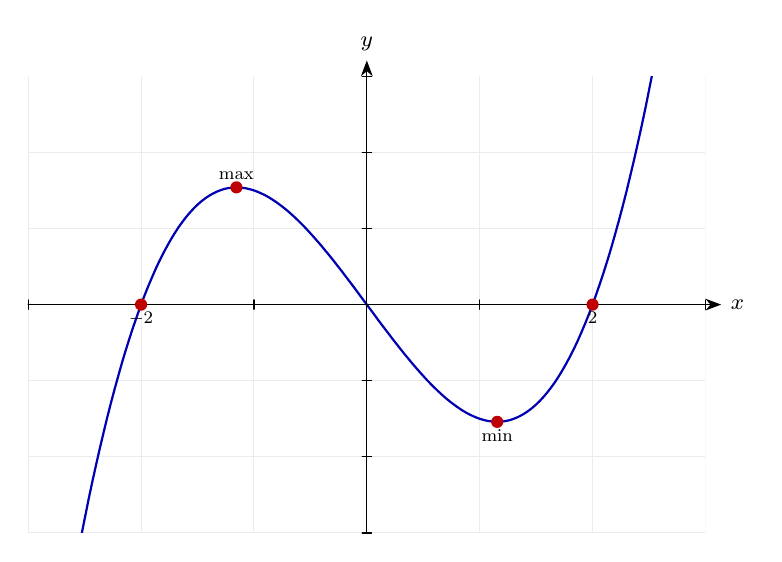
\begin{tikzpicture}[>={Stealth[length=2mm]},font=\footnotesize,line cap=round,line join=round]
\begin{scope}
\clip (0,0) rectangle (8.6,5.8);
\draw[gray!16] (0,0) grid[xstep=1.433,ystep=0.967] (8.6,5.8);
\draw[blue!70!black,thick] (0,-4.35) -- (0.048,-3.984) -- (0.096,-3.628) -- (0.143,-3.281) -- (0.191,-2.944) -- (0.239,-2.616) -- (0.287,-2.297) -- (0.334,-1.987) -- (0.382,-1.686) -- (0.43,-1.393) -- (0.478,-1.11) -- (0.526,-0.835) -- (0.573,-0.568) -- (0.621,-0.31) -- (0.669,-0.06) -- (0.717,0.181) -- (0.764,0.415) -- (0.812,0.641) -- (0.86,0.858) -- (0.908,1.069) -- (0.956,1.271) -- (1.003,1.466) -- (1.051,1.654) -- (1.099,1.834) -- (1.147,2.007) -- (1.194,2.173) -- (1.242,2.332) -- (1.29,2.484) -- (1.338,2.629) -- (1.386,2.768) -- (1.433,2.9) -- (1.481,3.026) -- (1.529,3.145) -- (1.577,3.258) -- (1.624,3.365) -- (1.672,3.466) -- (1.72,3.561) -- (1.768,3.65) -- (1.816,3.734) -- (1.863,3.812) -- (1.911,3.885) -- (1.959,3.952) -- (2.007,4.014) -- (2.054,4.07) -- (2.102,4.122) -- (2.15,4.169) -- (2.198,4.211) -- (2.246,4.248) -- (2.293,4.28) -- (2.341,4.308) -- (2.389,4.332) -- (2.437,4.351) -- (2.484,4.367) -- (2.532,4.378) -- (2.58,4.385) -- (2.628,4.388) -- (2.676,4.388) -- (2.723,4.383) -- (2.771,4.376) -- (2.819,4.364) -- (2.867,4.35) -- (2.914,4.332) -- (2.962,4.311) -- (3.01,4.288) -- (3.058,4.261) -- (3.106,4.231) -- (3.153,4.199) -- (3.201,4.164) -- (3.249,4.127) -- (3.297,4.088) -- (3.344,4.046) -- (3.392,4.002) -- (3.44,3.956) -- (3.488,3.908) -- (3.536,3.858) -- (3.583,3.806) -- (3.631,3.753) -- (3.679,3.698) -- (3.727,3.642) -- (3.774,3.585) -- (3.822,3.527) -- (3.87,3.467) -- (3.918,3.406) -- (3.966,3.345) -- (4.013,3.283) -- (4.061,3.22) -- (4.109,3.157) -- (4.157,3.093) -- (4.204,3.029) -- (4.252,2.964) -- (4.3,2.9) -- (4.348,2.836) -- (4.396,2.771) -- (4.443,2.707) -- (4.491,2.643) -- (4.539,2.58) -- (4.587,2.517) -- (4.634,2.455) -- (4.682,2.394) -- (4.73,2.333) -- (4.778,2.273) -- (4.826,2.215) -- (4.873,2.158) -- (4.921,2.102) -- (4.969,2.047) -- (5.017,1.994) -- (5.064,1.942) -- (5.112,1.892) -- (5.16,1.844) -- (5.208,1.798) -- (5.256,1.754) -- (5.303,1.712) -- (5.351,1.673) -- (5.399,1.636) -- (5.447,1.601) -- (5.494,1.569) -- (5.542,1.539) -- (5.59,1.512) -- (5.638,1.489) -- (5.686,1.468) -- (5.733,1.45) -- (5.781,1.436) -- (5.829,1.424) -- (5.877,1.417) -- (5.924,1.412) -- (5.972,1.412) -- (6.02,1.415) -- (6.068,1.422) -- (6.116,1.433) -- (6.163,1.449) -- (6.211,1.468) -- (6.259,1.492) -- (6.307,1.52) -- (6.354,1.552) -- (6.402,1.589) -- (6.45,1.631) -- (6.498,1.678) -- (6.546,1.73) -- (6.593,1.786) -- (6.641,1.848) -- (6.689,1.915) -- (6.737,1.988) -- (6.784,2.066) -- (6.832,2.15) -- (6.88,2.239) -- (6.928,2.334) -- (6.976,2.435) -- (7.023,2.542) -- (7.071,2.655) -- (7.119,2.774) -- (7.167,2.9) -- (7.214,3.032) -- (7.262,3.171) -- (7.31,3.316) -- (7.358,3.468) -- (7.406,3.627) -- (7.453,3.793) -- (7.501,3.966) -- (7.549,4.146) -- (7.597,4.334) -- (7.644,4.529) -- (7.692,4.731) -- (7.74,4.942) -- (7.788,5.159) -- (7.836,5.385) -- (7.883,5.619) -- (7.931,5.86) -- (7.979,6.11) -- (8.027,6.368) -- (8.074,6.635) -- (8.122,6.91) -- (8.17,7.193) -- (8.218,7.486) -- (8.266,7.787) -- (8.313,8.097) -- (8.361,8.416) -- (8.409,8.744) -- (8.457,9.081) -- (8.504,9.428) -- (8.552,9.784) -- (8.6,10.15);
\end{scope}
\draw[->] (0,2.9) -- (8.8,2.9) node[right]{$x$};
\draw[->] (4.3,0) -- (4.3,6) node[above]{$y$};
\draw (0,2.84) -- (0,2.96);
\draw (1.433,2.84) -- (1.433,2.96);
\draw (2.867,2.84) -- (2.867,2.96);
\draw (5.733,2.84) -- (5.733,2.96);
\draw (7.167,2.84) -- (7.167,2.96);
\draw (8.6,2.84) -- (8.6,2.96);
\draw (4.24,0) -- (4.36,0);
\draw (4.24,0.967) -- (4.36,0.967);
\draw (4.24,1.933) -- (4.36,1.933);
\draw (4.24,3.867) -- (4.36,3.867);
\draw (4.24,4.833) -- (4.36,4.833);
\draw (4.24,5.8) -- (4.36,5.8);
\fill[red!75!black] (5.956,1.411) circle (2.2pt);
\node[below,scale=0.8] at (5.956,1.411) {min};
\fill[red!75!black] (2.644,4.389) circle (2.2pt);
\node[above,scale=0.8] at (2.644,4.389) {max};
\fill[red!75!black] (1.433,2.9) circle (2.2pt);
\node[below,scale=0.8] at (1.433,2.9) {$-2$};
\fill[red!75!black] (7.167,2.9) circle (2.2pt);
\node[below,scale=0.8] at (7.167,2.9) {$2$};
\end{tikzpicture}
}
\end{center}
\small Curve with classified stationary points marked.\normalsize

\medskip\hrule

\section*{Derivatives and Graphs 21\quad\small\texttt{(d4-021)}}
\addcontentsline{toc}{section}{Derivatives and Graphs 21 (d4-021)}
\textit{Difficulty: Foundation \quad\textbar\quad Marks: 6}

\question{Sketch the curve \( y = x^3 + 3x^2 \), labelling the coordinates of all stationary points and axis intercepts.}

\textbf{Worked solution.}

\textit{Step 1: Find axis intercepts.}
\[\begin{gathered}
y\text{-intercept}: x=0 \Rightarrow y=0 \newline x\text{-intercepts}: x^2(x+3)=0 \Rightarrow x=0 \text{ (double root)},\; x=-3
\end{gathered}\]
The double root at \(0\) means the curve touches but does not cross the \(x\)-axis there.

\textit{Step 2: Find stationary points.}
\[\begin{gathered}
\frac{\mathrm{d}y}{\mathrm{d}x} = 3x^2 + 6x = 3x(x+2) = 0 \implies x=0 \text{ or } x=-2
\end{gathered}\]
Set \( \dfrac{\mathrm{d}y}{\mathrm{d}x} = 0 \).

\textit{Step 3: Coordinates.}
\[\begin{gathered}
x=0: y=0; \quad x=-2: y = -8 + 12 = 4
\end{gathered}\]
Substitute back into \( y \).

\textit{Step 4: Classify.}
\[\begin{gathered}
\frac{\mathrm{d}^2y}{\mathrm{d}x^2} = 6x + 6 \newline x=0: 6>0 \Rightarrow \text{minimum} \newline x=-2: -6<0 \Rightarrow \text{maximum}
\end{gathered}\]
Second derivative test.

\textit{Step 5: Overall shape.}
\[\begin{gathered}
\text{Cubic with positive leading coefficient; rises left-to-right.}
\end{gathered}\]
Crosses \(x\)-axis at \((-3, 0)\), touches at \((0, 0)\); local max at \((-2, 4)\), local min at \((0, 0)\).

\begin{answerbox}
\textbf{Final answer:}\quad Intercepts: \(\displaystyle  (-3, 0) \) and \(\displaystyle  (0, 0) \). Local maximum at \(\displaystyle  (-2, 4) \); local minimum at \(\displaystyle  (0, 0) \).
\end{answerbox}
\textbf{Diagram.}

\begin{center}
\resizebox{\ifdim\width>\linewidth \linewidth\else \width\fi}{!}{%
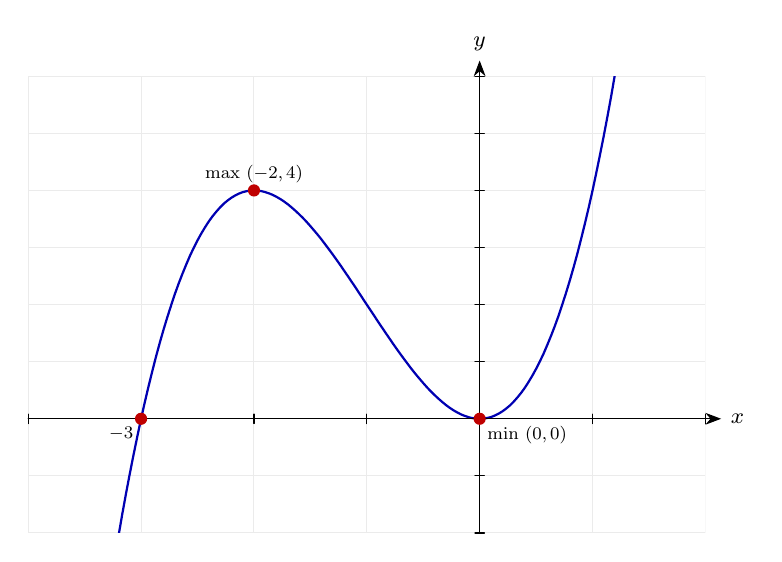
\begin{tikzpicture}[>={Stealth[length=2mm]},font=\footnotesize,line cap=round,line join=round]
\begin{scope}
\clip (0,0) rectangle (8.6,5.8);
\draw[gray!16] (0,0) grid[xstep=1.433,ystep=0.725] (8.6,5.8);
\draw[blue!70!black,thick] (0,-5.8) -- (0.048,-5.8) -- (0.096,-5.8) -- (0.143,-5.8) -- (0.191,-5.8) -- (0.239,-5.8) -- (0.287,-5.8) -- (0.334,-5.8) -- (0.382,-5.8) -- (0.43,-5.498) -- (0.478,-5.048) -- (0.526,-4.612) -- (0.573,-4.188) -- (0.621,-3.776) -- (0.669,-3.377) -- (0.717,-2.991) -- (0.764,-2.616) -- (0.812,-2.253) -- (0.86,-1.902) -- (0.908,-1.563) -- (0.956,-1.235) -- (1.003,-0.919) -- (1.051,-0.613) -- (1.099,-0.319) -- (1.147,-0.035) -- (1.194,0.238) -- (1.242,0.501) -- (1.29,0.753) -- (1.338,0.995) -- (1.386,1.228) -- (1.433,1.45) -- (1.481,1.663) -- (1.529,1.866) -- (1.577,2.06) -- (1.624,2.244) -- (1.672,2.42) -- (1.72,2.587) -- (1.768,2.745) -- (1.816,2.894) -- (1.863,3.036) -- (1.911,3.169) -- (1.959,3.293) -- (2.007,3.41) -- (2.054,3.52) -- (2.102,3.621) -- (2.15,3.716) -- (2.198,3.803) -- (2.246,3.883) -- (2.293,3.956) -- (2.341,4.022) -- (2.389,4.081) -- (2.437,4.135) -- (2.484,4.182) -- (2.532,4.222) -- (2.58,4.257) -- (2.628,4.286) -- (2.676,4.31) -- (2.723,4.328) -- (2.771,4.34) -- (2.819,4.348) -- (2.867,4.35) -- (2.914,4.348) -- (2.962,4.341) -- (3.01,4.329) -- (3.058,4.313) -- (3.106,4.293) -- (3.153,4.269) -- (3.201,4.241) -- (3.249,4.209) -- (3.297,4.174) -- (3.344,4.135) -- (3.392,4.093) -- (3.44,4.048) -- (3.488,4.001) -- (3.536,3.95) -- (3.583,3.897) -- (3.631,3.841) -- (3.679,3.784) -- (3.727,3.724) -- (3.774,3.662) -- (3.822,3.598) -- (3.87,3.533) -- (3.918,3.466) -- (3.966,3.398) -- (4.013,3.329) -- (4.061,3.259) -- (4.109,3.188) -- (4.157,3.117) -- (4.204,3.045) -- (4.252,2.972) -- (4.3,2.9) -- (4.348,2.828) -- (4.396,2.755) -- (4.443,2.683) -- (4.491,2.612) -- (4.539,2.541) -- (4.587,2.471) -- (4.634,2.402) -- (4.682,2.334) -- (4.73,2.267) -- (4.778,2.202) -- (4.826,2.138) -- (4.873,2.076) -- (4.921,2.016) -- (4.969,1.959) -- (5.017,1.903) -- (5.064,1.85) -- (5.112,1.799) -- (5.16,1.752) -- (5.208,1.707) -- (5.256,1.665) -- (5.303,1.626) -- (5.351,1.591) -- (5.399,1.559) -- (5.447,1.531) -- (5.494,1.507) -- (5.542,1.487) -- (5.59,1.471) -- (5.638,1.459) -- (5.686,1.452) -- (5.733,1.45) -- (5.781,1.452) -- (5.829,1.46) -- (5.877,1.472) -- (5.924,1.49) -- (5.972,1.514) -- (6.02,1.543) -- (6.068,1.578) -- (6.116,1.618) -- (6.163,1.665) -- (6.211,1.719) -- (6.259,1.778) -- (6.307,1.844) -- (6.354,1.917) -- (6.402,1.997) -- (6.45,2.084) -- (6.498,2.179) -- (6.546,2.28) -- (6.593,2.39) -- (6.641,2.507) -- (6.689,2.631) -- (6.737,2.764) -- (6.784,2.906) -- (6.832,3.055) -- (6.88,3.213) -- (6.928,3.38) -- (6.976,3.556) -- (7.023,3.74) -- (7.071,3.934) -- (7.119,4.137) -- (7.167,4.35) -- (7.214,4.572) -- (7.262,4.805) -- (7.31,5.047) -- (7.358,5.299) -- (7.406,5.562) -- (7.453,5.835) -- (7.501,6.119) -- (7.549,6.413) -- (7.597,6.719) -- (7.644,7.035) -- (7.692,7.363) -- (7.74,7.702) -- (7.788,8.053) -- (7.836,8.416) -- (7.883,8.791) -- (7.931,9.177) -- (7.979,9.576) -- (8.027,9.988) -- (8.074,10.412) -- (8.122,10.848) -- (8.17,11.298) -- (8.218,11.6) -- (8.266,11.6) -- (8.313,11.6) -- (8.361,11.6) -- (8.409,11.6) -- (8.457,11.6) -- (8.504,11.6) -- (8.552,11.6) -- (8.6,11.6);
\end{scope}
\draw[->] (0,1.45) -- (8.8,1.45) node[right]{$x$};
\draw[->] (5.733,0) -- (5.733,6) node[above]{$y$};
\draw (0,1.39) -- (0,1.51);
\draw (1.433,1.39) -- (1.433,1.51);
\draw (2.867,1.39) -- (2.867,1.51);
\draw (4.3,1.39) -- (4.3,1.51);
\draw (7.167,1.39) -- (7.167,1.51);
\draw (8.6,1.39) -- (8.6,1.51);
\draw (5.673,0) -- (5.793,0);
\draw (5.673,0.725) -- (5.793,0.725);
\draw (5.673,2.175) -- (5.793,2.175);
\draw (5.673,2.9) -- (5.793,2.9);
\draw (5.673,3.625) -- (5.793,3.625);
\draw (5.673,4.35) -- (5.793,4.35);
\draw (5.673,5.075) -- (5.793,5.075);
\draw (5.673,5.8) -- (5.793,5.8);
\fill[red!75!black] (2.867,4.35) circle (2.2pt);
\node[above,scale=0.8] at (2.867,4.35) {max $(-2,4)$};
\fill[red!75!black] (5.733,1.45) circle (2.2pt);
\node[below right,scale=0.8] at (5.733,1.45) {min $(0,0)$};
\fill[red!75!black] (1.433,1.45) circle (2.2pt);
\node[below left,scale=0.8] at (1.433,1.45) {$-3$};
\end{tikzpicture}
}
\end{center}
\small Curve with classified stationary points marked.\normalsize

\medskip\hrule

\section*{Derivatives and Graphs 22\quad\small\texttt{(d4-022)}}
\addcontentsline{toc}{section}{Derivatives and Graphs 22 (d4-022)}
\textit{Difficulty: Foundation \quad\textbar\quad Marks: 6}

\question{For the function \( f(x) = x^3 + 2x^2 - 4x + 1 \): (a) Find \( f'(x) \). (b) Find the range of values of \( x \) for which \( f \) is increasing. (c) Find the range of values of \( x \) for which \( f \) is decreasing.}

\textbf{Worked solution.}

\textit{Step 1: (a) Differentiate.}
\[\begin{gathered}
f'(x) = 3x^2 + 4x - 4
\end{gathered}\]
Power rule.

\textit{Step 2: Factorise \( f'(x) \).}
\[\begin{gathered}
f'(x) = (3x - 2)(x + 2)
\end{gathered}\]
Find factors of \( 3 \times (-4) = -12 \) that add to \( 4 \): these are \( 6 \) and \( -2 \).

\textit{Step 3: (b) Increasing: \( f'(x) > 0 \).}
\[\begin{gathered}
(3x-2)(x+2) > 0 \implies x < -2 \text{ or } x > \tfrac{2}{3}
\end{gathered}\]
Both factors positive or both negative.

\textit{Step 4: (c) Decreasing: \( f'(x) < 0 \).}
\[\begin{gathered}
-2 < x < \tfrac{2}{3}
\end{gathered}\]
Between the roots of \( f'(x) = 0 \), the product is negative.

\begin{answerbox}
\textbf{Final answer:}\quad (a) \(\displaystyle  f'(x) = (3x-2)(x+2) \) \\[3pt]  (b) Increasing: \(\displaystyle  x < -2 \) or \(\displaystyle  x > \tfrac{2}{3} \) \\[3pt]  (c) Decreasing: \(\displaystyle  -2 < x < \tfrac{2}{3} \)
\end{answerbox}
\textbf{Diagram.}

\begin{center}
\resizebox{\ifdim\width>\linewidth \linewidth\else \width\fi}{!}{%
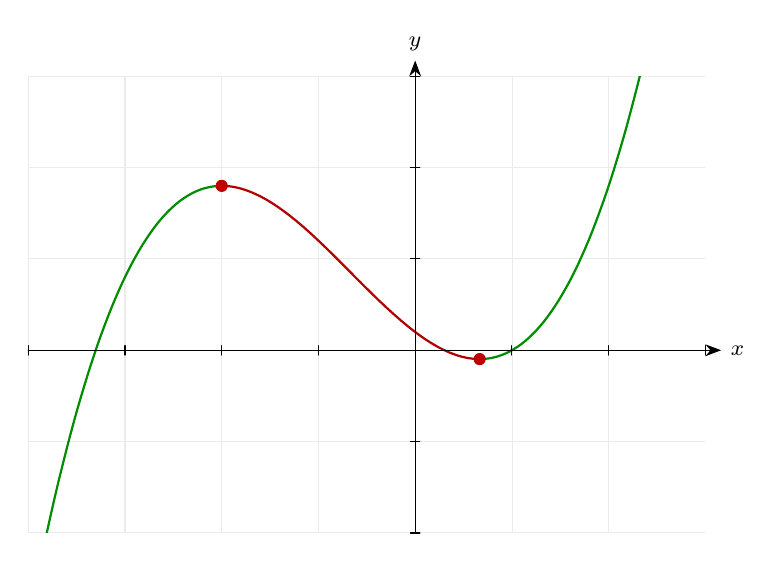
\begin{tikzpicture}[>={Stealth[length=2mm]},font=\footnotesize,line cap=round,line join=round]
\begin{scope}
\clip (0,0) rectangle (8.6,5.8);
\draw[gray!16] (0,0) grid[xstep=1.229,ystep=1.16] (8.6,5.8);
\draw[green!55!black,thick] (0,-1.16) -- (0.048,-0.909) -- (0.096,-0.665) -- (0.145,-0.427) -- (0.193,-0.197) -- (0.241,0.026) -- (0.289,0.243) -- (0.337,0.453) -- (0.385,0.657) -- (0.434,0.854) -- (0.482,1.045) -- (0.53,1.229) -- (0.578,1.407) -- (0.626,1.579) -- (0.675,1.746) -- (0.723,1.906) -- (0.771,2.06) -- (0.819,2.208) -- (0.867,2.351) -- (0.915,2.488) -- (0.964,2.62) -- (1.012,2.746) -- (1.06,2.867) -- (1.108,2.982) -- (1.156,3.092) -- (1.204,3.197) -- (1.253,3.297) -- (1.301,3.393) -- (1.349,3.483) -- (1.397,3.568) -- (1.445,3.649) -- (1.494,3.725) -- (1.542,3.797) -- (1.59,3.864) -- (1.638,3.927) -- (1.686,3.985) -- (1.734,4.04) -- (1.783,4.09) -- (1.831,4.136) -- (1.879,4.178) -- (1.927,4.217) -- (1.975,4.251) -- (2.024,4.282) -- (2.072,4.309) -- (2.12,4.333) -- (2.168,4.354) -- (2.216,4.371) -- (2.264,4.384) -- (2.313,4.395) -- (2.361,4.402) -- (2.409,4.407) -- (2.457,4.408);
\draw[red!70!black,thick] (2.457,4.408) -- (2.505,4.407) -- (2.552,4.403) -- (2.6,4.396) -- (2.647,4.387) -- (2.695,4.375) -- (2.742,4.361) -- (2.79,4.345) -- (2.837,4.326) -- (2.884,4.305) -- (2.932,4.283) -- (2.979,4.258) -- (3.027,4.232) -- (3.074,4.203) -- (3.122,4.173) -- (3.169,4.141) -- (3.217,4.108) -- (3.264,4.073) -- (3.312,4.037) -- (3.359,3.999) -- (3.407,3.961) -- (3.454,3.921) -- (3.502,3.88) -- (3.549,3.838) -- (3.597,3.795) -- (3.644,3.751) -- (3.692,3.706) -- (3.739,3.661) -- (3.787,3.615) -- (3.834,3.569) -- (3.882,3.522) -- (3.929,3.475) -- (3.977,3.427) -- (4.024,3.38) -- (4.071,3.332) -- (4.119,3.284) -- (4.166,3.236) -- (4.214,3.189) -- (4.261,3.141) -- (4.309,3.094) -- (4.356,3.047) -- (4.404,3.001) -- (4.451,2.955) -- (4.499,2.91) -- (4.546,2.865) -- (4.594,2.822) -- (4.641,2.779) -- (4.689,2.737) -- (4.736,2.696) -- (4.784,2.656) -- (4.831,2.617) -- (4.879,2.579) -- (4.926,2.543) -- (4.974,2.508) -- (5.021,2.475) -- (5.069,2.443) -- (5.116,2.413) -- (5.164,2.385) -- (5.211,2.358) -- (5.259,2.334) -- (5.306,2.311) -- (5.353,2.29) -- (5.401,2.272) -- (5.448,2.255) -- (5.496,2.241) -- (5.543,2.23) -- (5.591,2.22) -- (5.638,2.214) -- (5.686,2.21) -- (5.733,2.208);
\draw[green!55!black,thick] (5.733,2.208) -- (5.781,2.21) -- (5.829,2.214) -- (5.877,2.221) -- (5.924,2.232) -- (5.972,2.245) -- (6.02,2.262) -- (6.068,2.282) -- (6.116,2.305) -- (6.163,2.332) -- (6.211,2.362) -- (6.259,2.396) -- (6.307,2.434) -- (6.354,2.475) -- (6.402,2.521) -- (6.45,2.57) -- (6.498,2.623) -- (6.546,2.681) -- (6.593,2.743) -- (6.641,2.809) -- (6.689,2.879) -- (6.737,2.954) -- (6.784,3.033) -- (6.832,3.117) -- (6.88,3.205) -- (6.928,3.299) -- (6.976,3.397) -- (7.023,3.5) -- (7.071,3.608) -- (7.119,3.721) -- (7.167,3.84) -- (7.214,3.964) -- (7.262,4.093) -- (7.31,4.227) -- (7.358,4.367) -- (7.406,4.513) -- (7.453,4.664) -- (7.501,4.821) -- (7.549,4.984) -- (7.597,5.152) -- (7.644,5.327) -- (7.692,5.508) -- (7.74,5.695) -- (7.788,5.888) -- (7.836,6.088) -- (7.883,6.294) -- (7.931,6.506) -- (7.979,6.725) -- (8.027,6.951) -- (8.074,7.183) -- (8.122,7.423) -- (8.17,7.669) -- (8.218,7.922) -- (8.266,8.182) -- (8.313,8.449) -- (8.361,8.724) -- (8.409,9.006) -- (8.457,9.295) -- (8.504,9.592) -- (8.552,9.896) -- (8.6,10.208);
\end{scope}
\draw[->] (0,2.32) -- (8.8,2.32) node[right]{$x$};
\draw[->] (4.914,0) -- (4.914,6) node[above]{$y$};
\draw (0,2.26) -- (0,2.38);
\draw (1.229,2.26) -- (1.229,2.38);
\draw (2.457,2.26) -- (2.457,2.38);
\draw (3.686,2.26) -- (3.686,2.38);
\draw (6.143,2.26) -- (6.143,2.38);
\draw (7.371,2.26) -- (7.371,2.38);
\draw (8.6,2.26) -- (8.6,2.38);
\draw (4.854,0) -- (4.974,0);
\draw (4.854,1.16) -- (4.974,1.16);
\draw (4.854,3.48) -- (4.974,3.48);
\draw (4.854,4.64) -- (4.974,4.64);
\draw (4.854,5.8) -- (4.974,5.8);
\fill[red!75!black] (2.457,4.408) circle (2.2pt);
\fill[red!75!black] (5.733,2.208) circle (2.2pt);
\end{tikzpicture}
}
\end{center}
\small Curve coloured green where increasing, red where decreasing.\normalsize

\medskip\hrule

\section*{Derivatives and Graphs 23\quad\small\texttt{(d4-023)}}
\addcontentsline{toc}{section}{Derivatives and Graphs 23 (d4-023)}
\textit{Difficulty: Foundation \quad\textbar\quad Marks: 3}

\question{A function \( f \) satisfies \( f(2) = -3 \), \( f'(2) = 0 \) and \( f''(2) = 5 \). (a) Write down the coordinates of a stationary point of \( f \). (b) Determine its nature, giving a reason.}

\textbf{Worked solution.}

\textit{Step 1: (a) A stationary point occurs where \( f'(x) = 0 \).}
\[\begin{gathered}
f'(2) = 0, \text{ so the stationary point is at } (2, -3)
\end{gathered}\]
\( f(2) = -3 \) gives the \( y \)-coordinate.

\textit{Step 2: (b) Determine the nature.}
\[\begin{gathered}
f''(2) = 5 > 0 \Rightarrow \text{local minimum}
\end{gathered}\]
A positive second derivative at a stationary point confirms a local minimum.

\begin{answerbox}
\textbf{Final answer:}\quad (a) \(\displaystyle  (2, -3) \) \\[3pt]  (b) Local minimum, since \(\displaystyle  f''(2) = 5 > 0 \).
\end{answerbox}
\textbf{Diagram.}

\begin{center}
\resizebox{\ifdim\width>\linewidth \linewidth\else \width\fi}{!}{%
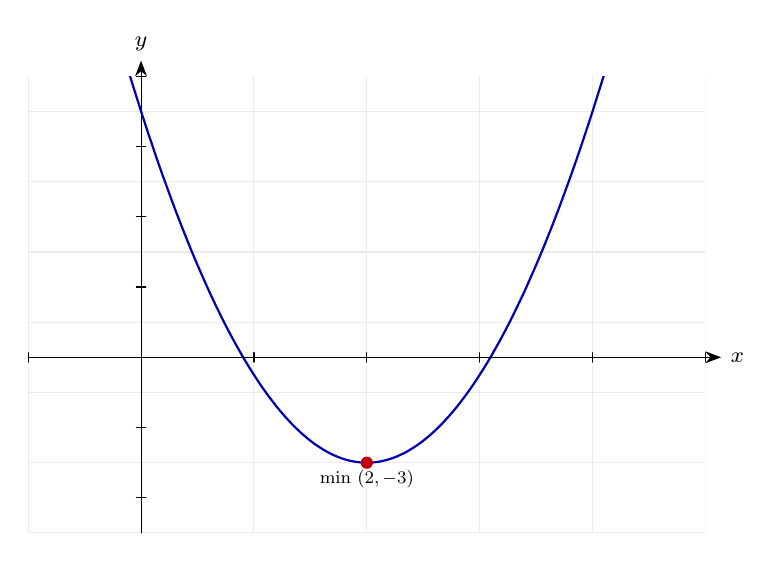
\begin{tikzpicture}[>={Stealth[length=2mm]},font=\footnotesize,line cap=round,line join=round]
\begin{scope}
\clip (0,0) rectangle (8.6,5.8);
\draw[gray!16] (0,-0.446) grid[xstep=1.433,ystep=0.892] (8.6,5.8);
\draw[blue!70!black,thick] (0,10.931) -- (0.048,10.709) -- (0.096,10.49) -- (0.143,10.273) -- (0.191,10.058) -- (0.239,9.846) -- (0.287,9.637) -- (0.334,9.43) -- (0.382,9.225) -- (0.43,9.023) -- (0.478,8.824) -- (0.526,8.627) -- (0.573,8.432) -- (0.621,8.24) -- (0.669,8.051) -- (0.717,7.863) -- (0.764,7.679) -- (0.812,7.497) -- (0.86,7.317) -- (0.908,7.14) -- (0.956,6.965) -- (1.003,6.793) -- (1.051,6.623) -- (1.099,6.456) -- (1.147,6.291) -- (1.194,6.128) -- (1.242,5.969) -- (1.29,5.811) -- (1.338,5.656) -- (1.386,5.504) -- (1.433,5.354) -- (1.481,5.206) -- (1.529,5.061) -- (1.577,4.919) -- (1.624,4.779) -- (1.672,4.641) -- (1.72,4.506) -- (1.768,4.374) -- (1.816,4.243) -- (1.863,4.116) -- (1.911,3.991) -- (1.959,3.868) -- (2.007,3.748) -- (2.054,3.63) -- (2.102,3.515) -- (2.15,3.402) -- (2.198,3.292) -- (2.246,3.184) -- (2.293,3.078) -- (2.341,2.976) -- (2.389,2.875) -- (2.437,2.777) -- (2.484,2.682) -- (2.532,2.589) -- (2.58,2.498) -- (2.628,2.41) -- (2.676,2.325) -- (2.723,2.242) -- (2.771,2.161) -- (2.819,2.083) -- (2.867,2.008) -- (2.914,1.935) -- (2.962,1.864) -- (3.01,1.796) -- (3.058,1.73) -- (3.106,1.667) -- (3.153,1.606) -- (3.201,1.548) -- (3.249,1.492) -- (3.297,1.439) -- (3.344,1.388) -- (3.392,1.34) -- (3.44,1.294) -- (3.488,1.25) -- (3.536,1.21) -- (3.583,1.171) -- (3.631,1.135) -- (3.679,1.102) -- (3.727,1.071) -- (3.774,1.042) -- (3.822,1.016) -- (3.87,0.993) -- (3.918,0.972) -- (3.966,0.953) -- (4.013,0.937) -- (4.061,0.923) -- (4.109,0.912) -- (4.157,0.903) -- (4.204,0.897) -- (4.252,0.894) -- (4.3,0.892) -- (4.348,0.894) -- (4.396,0.897) -- (4.443,0.903) -- (4.491,0.912) -- (4.539,0.923) -- (4.587,0.937) -- (4.634,0.953) -- (4.682,0.972) -- (4.73,0.993) -- (4.778,1.016) -- (4.826,1.042) -- (4.873,1.071) -- (4.921,1.102) -- (4.969,1.135) -- (5.017,1.171) -- (5.064,1.21) -- (5.112,1.25) -- (5.16,1.294) -- (5.208,1.34) -- (5.256,1.388) -- (5.303,1.439) -- (5.351,1.492) -- (5.399,1.548) -- (5.447,1.606) -- (5.494,1.667) -- (5.542,1.73) -- (5.59,1.796) -- (5.638,1.864) -- (5.686,1.935) -- (5.733,2.008) -- (5.781,2.083) -- (5.829,2.161) -- (5.877,2.242) -- (5.924,2.325) -- (5.972,2.41) -- (6.02,2.498) -- (6.068,2.589) -- (6.116,2.682) -- (6.163,2.777) -- (6.211,2.875) -- (6.259,2.976) -- (6.307,3.078) -- (6.354,3.184) -- (6.402,3.292) -- (6.45,3.402) -- (6.498,3.515) -- (6.546,3.63) -- (6.593,3.748) -- (6.641,3.868) -- (6.689,3.991) -- (6.737,4.116) -- (6.784,4.243) -- (6.832,4.374) -- (6.88,4.506) -- (6.928,4.641) -- (6.976,4.779) -- (7.023,4.919) -- (7.071,5.061) -- (7.119,5.206) -- (7.167,5.354) -- (7.214,5.504) -- (7.262,5.656) -- (7.31,5.811) -- (7.358,5.969) -- (7.406,6.128) -- (7.453,6.291) -- (7.501,6.456) -- (7.549,6.623) -- (7.597,6.793) -- (7.644,6.965) -- (7.692,7.14) -- (7.74,7.317) -- (7.788,7.497) -- (7.836,7.679) -- (7.883,7.863) -- (7.931,8.051) -- (7.979,8.24) -- (8.027,8.432) -- (8.074,8.627) -- (8.122,8.824) -- (8.17,9.023) -- (8.218,9.225) -- (8.266,9.43) -- (8.313,9.637) -- (8.361,9.846) -- (8.409,10.058) -- (8.457,10.273) -- (8.504,10.49) -- (8.552,10.709) -- (8.6,10.931);
\end{scope}
\draw[->] (0,2.231) -- (8.8,2.231) node[right]{$x$};
\draw[->] (1.433,0) -- (1.433,6) node[above]{$y$};
\draw (0,2.171) -- (0,2.291);
\draw (2.867,2.171) -- (2.867,2.291);
\draw (4.3,2.171) -- (4.3,2.291);
\draw (5.733,2.171) -- (5.733,2.291);
\draw (7.167,2.171) -- (7.167,2.291);
\draw (8.6,2.171) -- (8.6,2.291);
\draw (1.373,0.446) -- (1.493,0.446);
\draw (1.373,1.338) -- (1.493,1.338);
\draw (1.373,3.123) -- (1.493,3.123);
\draw (1.373,4.015) -- (1.493,4.015);
\draw (1.373,4.908) -- (1.493,4.908);
\draw (1.373,5.8) -- (1.493,5.8);
\fill[red!75!black] (4.3,0.892) circle (2.2pt);
\node[below,scale=0.8] at (4.3,0.892) {min $(2,-3)$};
\end{tikzpicture}
}
\end{center}
\small Curve with classified stationary points marked.\normalsize

\medskip\hrule

\section*{Derivatives and Graphs 24\quad\small\texttt{(d4-024)}}
\addcontentsline{toc}{section}{Derivatives and Graphs 24 (d4-024)}
\textit{Difficulty: Foundation \quad\textbar\quad Marks: 5}

\question{A function is given by \( y = x^3 + ax^2 + bx + 5 \). The curve has a stationary point at \( (1, 4) \). Find the values of \( a \) and \( b \).}

\textbf{Worked solution.}

\textit{Step 1: Since \( (1, 4) \) lies on the curve, substitute \( x = 1 \), \( y = 4 \).}
\[\begin{gathered}
1 + a + b + 5 = 4 \implies a + b = -2 \quad \cdots (1)
\end{gathered}\]
This gives one equation in \( a \) and \( b \).

\textit{Step 2: Differentiate.}
\[\begin{gathered}
\frac{\mathrm{d}y}{\mathrm{d}x} = 3x^2 + 2ax + b
\end{gathered}\]
Power rule.

\textit{Step 3: At a stationary point \( \dfrac{\mathrm{d}y}{\mathrm{d}x} = 0 \) when \( x = 1 \).}
\[\begin{gathered}
3 + 2a + b = 0 \implies 2a + b = -3 \quad \cdots (2)
\end{gathered}\]
This gives a second equation.

\textit{Step 4: Solve simultaneously: subtract (1) from (2).}
\[\begin{gathered}
(2a + b) - (a + b) = -3 - (-2) \implies a = -1
\end{gathered}\]
Eliminate \( b \).

\textit{Step 5: Back-substitute into (1).}
\[\begin{gathered}
-1 + b = -2 \implies b = -1
\end{gathered}\]
Solve for \( b \).

\begin{answerbox}
\textbf{Final answer:}\quad \(\displaystyle  a = -1,\; b = -1 \)
\end{answerbox}
\textbf{Diagram.}

\begin{center}
\resizebox{\ifdim\width>\linewidth \linewidth\else \width\fi}{!}{%
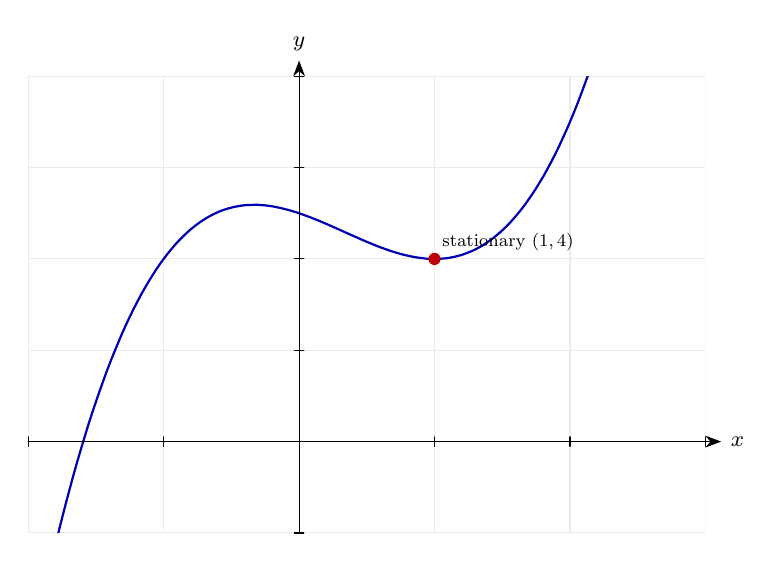
\begin{tikzpicture}[>={Stealth[length=2mm]},font=\footnotesize,line cap=round,line join=round]
\begin{scope}
\clip (0,0) rectangle (8.6,5.8);
\draw[gray!16] (0,0) grid[xstep=1.72,ystep=1.16] (8.6,5.8);
\draw[blue!70!black,thick] (0,-1.74) -- (0.048,-1.501) -- (0.096,-1.269) -- (0.143,-1.043) -- (0.191,-0.823) -- (0.239,-0.608) -- (0.287,-0.4) -- (0.334,-0.198) -- (0.382,-0.001) -- (0.43,0.19) -- (0.478,0.376) -- (0.526,0.556) -- (0.573,0.73) -- (0.621,0.9) -- (0.669,1.063) -- (0.717,1.222) -- (0.764,1.376) -- (0.812,1.524) -- (0.86,1.667) -- (0.908,1.806) -- (0.956,1.94) -- (1.003,2.069) -- (1.051,2.193) -- (1.099,2.312) -- (1.147,2.427) -- (1.194,2.538) -- (1.242,2.644) -- (1.29,2.746) -- (1.338,2.844) -- (1.386,2.937) -- (1.433,3.026) -- (1.481,3.111) -- (1.529,3.193) -- (1.577,3.27) -- (1.624,3.344) -- (1.672,3.414) -- (1.72,3.48) -- (1.768,3.543) -- (1.816,3.602) -- (1.863,3.658) -- (1.911,3.71) -- (1.959,3.759) -- (2.007,3.805) -- (2.054,3.848) -- (2.102,3.887) -- (2.15,3.924) -- (2.198,3.958) -- (2.246,3.989) -- (2.293,4.017) -- (2.341,4.043) -- (2.389,4.065) -- (2.437,4.086) -- (2.484,4.104) -- (2.532,4.119) -- (2.58,4.132) -- (2.628,4.143) -- (2.676,4.152) -- (2.723,4.159) -- (2.771,4.164) -- (2.819,4.166) -- (2.867,4.167) -- (2.914,4.167) -- (2.962,4.164) -- (3.01,4.16) -- (3.058,4.154) -- (3.106,4.147) -- (3.153,4.138) -- (3.201,4.128) -- (3.249,4.116) -- (3.297,4.104) -- (3.344,4.09) -- (3.392,4.076) -- (3.44,4.06) -- (3.488,4.043) -- (3.536,4.026) -- (3.583,4.008) -- (3.631,3.989) -- (3.679,3.97) -- (3.727,3.95) -- (3.774,3.93) -- (3.822,3.909) -- (3.87,3.888) -- (3.918,3.867) -- (3.966,3.845) -- (4.013,3.824) -- (4.061,3.802) -- (4.109,3.781) -- (4.157,3.76) -- (4.204,3.739) -- (4.252,3.718) -- (4.3,3.697) -- (4.348,3.678) -- (4.396,3.658) -- (4.443,3.639) -- (4.491,3.621) -- (4.539,3.604) -- (4.587,3.587) -- (4.634,3.572) -- (4.682,3.557) -- (4.73,3.543) -- (4.778,3.531) -- (4.826,3.52) -- (4.873,3.51) -- (4.921,3.501) -- (4.969,3.494) -- (5.017,3.488) -- (5.064,3.483) -- (5.112,3.481) -- (5.16,3.48) -- (5.208,3.481) -- (5.256,3.484) -- (5.303,3.488) -- (5.351,3.495) -- (5.399,3.504) -- (5.447,3.515) -- (5.494,3.528) -- (5.542,3.544) -- (5.59,3.562) -- (5.638,3.582) -- (5.686,3.605) -- (5.733,3.63) -- (5.781,3.659) -- (5.829,3.69) -- (5.877,3.723) -- (5.924,3.76) -- (5.972,3.8) -- (6.02,3.842) -- (6.068,3.888) -- (6.116,3.937) -- (6.163,3.99) -- (6.211,4.046) -- (6.259,4.105) -- (6.307,4.167) -- (6.354,4.234) -- (6.402,4.304) -- (6.45,4.377) -- (6.498,4.455) -- (6.546,4.536) -- (6.593,4.621) -- (6.641,4.71) -- (6.689,4.804) -- (6.737,4.901) -- (6.784,5.003) -- (6.832,5.109) -- (6.88,5.22) -- (6.928,5.335) -- (6.976,5.455) -- (7.023,5.579) -- (7.071,5.708) -- (7.119,5.841) -- (7.167,5.98) -- (7.214,6.123) -- (7.262,6.272) -- (7.31,6.425) -- (7.358,6.584) -- (7.406,6.748) -- (7.453,6.917) -- (7.501,7.092) -- (7.549,7.272) -- (7.597,7.457) -- (7.644,7.648) -- (7.692,7.845) -- (7.74,8.047) -- (7.788,8.256) -- (7.836,8.47) -- (7.883,8.69) -- (7.931,8.917) -- (7.979,9.149) -- (8.027,9.387) -- (8.074,9.632) -- (8.122,9.883) -- (8.17,10.141) -- (8.218,10.405) -- (8.266,10.676) -- (8.313,10.953) -- (8.361,11.237) -- (8.409,11.528) -- (8.457,11.6) -- (8.504,11.6) -- (8.552,11.6) -- (8.6,11.6);
\end{scope}
\draw[->] (0,1.16) -- (8.8,1.16) node[right]{$x$};
\draw[->] (3.44,0) -- (3.44,6) node[above]{$y$};
\draw (0,1.1) -- (0,1.22);
\draw (1.72,1.1) -- (1.72,1.22);
\draw (5.16,1.1) -- (5.16,1.22);
\draw (6.88,1.1) -- (6.88,1.22);
\draw (8.6,1.1) -- (8.6,1.22);
\draw (3.38,0) -- (3.5,0);
\draw (3.38,2.32) -- (3.5,2.32);
\draw (3.38,3.48) -- (3.5,3.48);
\draw (3.38,4.64) -- (3.5,4.64);
\draw (3.38,5.8) -- (3.5,5.8);
\fill[red!75!black] (5.16,3.48) circle (2.2pt);
\node[above right,scale=0.8] at (5.16,3.48) {stationary $(1,4)$};
\end{tikzpicture}
}
\end{center}
\small Curve with classified stationary points marked.\normalsize

\medskip\hrule

\section*{Derivatives and Graphs 25\quad\small\texttt{(d4-025)}}
\addcontentsline{toc}{section}{Derivatives and Graphs 25 (d4-025)}
\textit{Difficulty: Foundation \quad\textbar\quad Marks: 6}

\question{For the curve \( y = 3x^2 - x^3 \): (a) Find the coordinates of both stationary points. (b) Find the range of values of \( x \) for which the curve is increasing.}

\textbf{Worked solution.}

\textit{Step 1: (a) Differentiate.}
\[\begin{gathered}
\frac{\mathrm{d}y}{\mathrm{d}x} = 6x - 3x^2 = 3x(2 - x)
\end{gathered}\]
Factorise the derivative.

\textit{Step 2: Stationary points.}
\[\begin{gathered}
3x(2-x) = 0 \implies x = 0 \text{ or } x = 2
\end{gathered}\]
Set equal to zero.

\textit{Step 3: Find \( y \)-coordinates.}
\[\begin{gathered}
y(0) = 0; \quad y(2) = 12 - 8 = 4
\end{gathered}\]
Substitute into the original.

\textit{Step 4: (b) Increasing when \( \dfrac{\mathrm{d}y}{\mathrm{d}x} > 0 \).}
\[\begin{gathered}
3x(2-x) > 0 \implies 0 < x < 2
\end{gathered}\]
The product is positive when both factors have the same sign. \( 3x > 0 \) and \( 2-x > 0 \) when \( 0 < x < 2 \).

\begin{answerbox}
\textbf{Final answer:}\quad (a) \(\displaystyle  (0, 0) \) and \(\displaystyle  (2, 4) \) \\[3pt]  (b) \(\displaystyle  0 < x < 2 \)
\end{answerbox}
\textbf{Diagram.}

\begin{center}
\resizebox{\ifdim\width>\linewidth \linewidth\else \width\fi}{!}{%
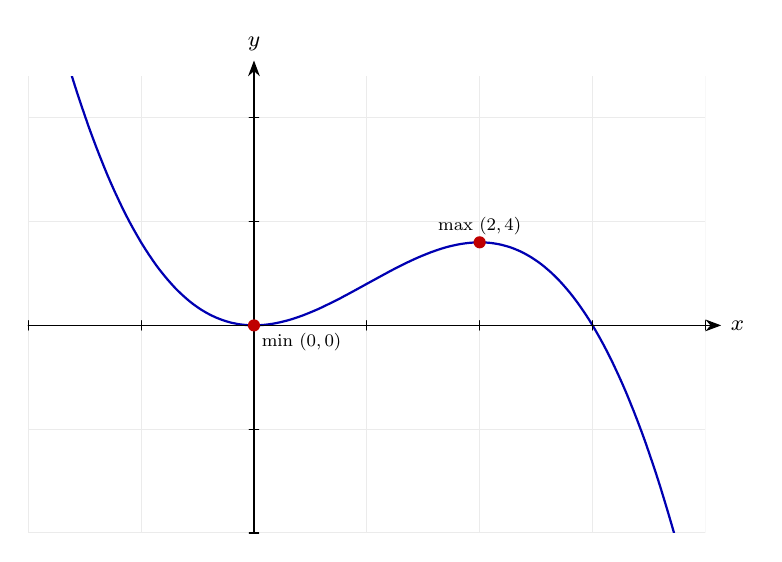
\begin{tikzpicture}[>={Stealth[length=2mm]},font=\footnotesize,line cap=round,line join=round]
\begin{scope}
\clip (0,0) rectangle (8.6,5.8);
\draw[gray!16] (0,0) grid[xstep=1.433,ystep=1.318] (8.6,5.8);
\draw[blue!70!black,thick] (0,7.909) -- (0.048,7.701) -- (0.096,7.498) -- (0.143,7.3) -- (0.191,7.107) -- (0.239,6.919) -- (0.287,6.736) -- (0.334,6.559) -- (0.382,6.386) -- (0.43,6.217) -- (0.478,6.054) -- (0.526,5.895) -- (0.573,5.741) -- (0.621,5.591) -- (0.669,5.446) -- (0.717,5.306) -- (0.764,5.169) -- (0.812,5.038) -- (0.86,4.91) -- (0.908,4.787) -- (0.956,4.667) -- (1.003,4.552) -- (1.051,4.441) -- (1.099,4.334) -- (1.147,4.231) -- (1.194,4.132) -- (1.242,4.036) -- (1.29,3.944) -- (1.338,3.856) -- (1.386,3.772) -- (1.433,3.691) -- (1.481,3.614) -- (1.529,3.54) -- (1.577,3.469) -- (1.624,3.402) -- (1.672,3.338) -- (1.72,3.278) -- (1.768,3.22) -- (1.816,3.166) -- (1.863,3.114) -- (1.911,3.066) -- (1.959,3.021) -- (2.007,2.978) -- (2.054,2.938) -- (2.102,2.901) -- (2.15,2.867) -- (2.198,2.835) -- (2.246,2.806) -- (2.293,2.78) -- (2.341,2.756) -- (2.389,2.734) -- (2.437,2.715) -- (2.484,2.698) -- (2.532,2.683) -- (2.58,2.67) -- (2.628,2.66) -- (2.676,2.651) -- (2.723,2.645) -- (2.771,2.64) -- (2.819,2.637) -- (2.867,2.636) -- (2.914,2.637) -- (2.962,2.64) -- (3.01,2.644) -- (3.058,2.65) -- (3.106,2.657) -- (3.153,2.666) -- (3.201,2.676) -- (3.249,2.688) -- (3.297,2.7) -- (3.344,2.714) -- (3.392,2.73) -- (3.44,2.746) -- (3.488,2.763) -- (3.536,2.782) -- (3.583,2.801) -- (3.631,2.821) -- (3.679,2.842) -- (3.727,2.864) -- (3.774,2.887) -- (3.822,2.91) -- (3.87,2.933) -- (3.918,2.958) -- (3.966,2.982) -- (4.013,3.008) -- (4.061,3.033) -- (4.109,3.059) -- (4.157,3.085) -- (4.204,3.111) -- (4.252,3.137) -- (4.3,3.164) -- (4.348,3.19) -- (4.396,3.216) -- (4.443,3.242) -- (4.491,3.268) -- (4.539,3.294) -- (4.587,3.32) -- (4.634,3.345) -- (4.682,3.37) -- (4.73,3.394) -- (4.778,3.418) -- (4.826,3.441) -- (4.873,3.463) -- (4.921,3.485) -- (4.969,3.506) -- (5.017,3.526) -- (5.064,3.545) -- (5.112,3.564) -- (5.16,3.581) -- (5.208,3.598) -- (5.256,3.613) -- (5.303,3.627) -- (5.351,3.64) -- (5.399,3.651) -- (5.447,3.661) -- (5.494,3.67) -- (5.542,3.677) -- (5.59,3.683) -- (5.638,3.687) -- (5.686,3.69) -- (5.733,3.691) -- (5.781,3.69) -- (5.829,3.687) -- (5.877,3.683) -- (5.924,3.676) -- (5.972,3.668) -- (6.02,3.657) -- (6.068,3.644) -- (6.116,3.63) -- (6.163,3.613) -- (6.211,3.593) -- (6.259,3.572) -- (6.307,3.547) -- (6.354,3.521) -- (6.402,3.492) -- (6.45,3.46) -- (6.498,3.426) -- (6.546,3.389) -- (6.593,3.349) -- (6.641,3.307) -- (6.689,3.261) -- (6.737,3.213) -- (6.784,3.162) -- (6.832,3.107) -- (6.88,3.05) -- (6.928,2.989) -- (6.976,2.925) -- (7.023,2.858) -- (7.071,2.788) -- (7.119,2.714) -- (7.167,2.636) -- (7.214,2.556) -- (7.262,2.471) -- (7.31,2.383) -- (7.358,2.291) -- (7.406,2.196) -- (7.453,2.096) -- (7.501,1.993) -- (7.549,1.886) -- (7.597,1.775) -- (7.644,1.66) -- (7.692,1.541) -- (7.74,1.417) -- (7.788,1.29) -- (7.836,1.158) -- (7.883,1.022) -- (7.931,0.881) -- (7.979,0.736) -- (8.027,0.586) -- (8.074,0.432) -- (8.122,0.273) -- (8.17,0.11) -- (8.218,-0.058) -- (8.266,-0.231) -- (8.313,-0.409) -- (8.361,-0.592) -- (8.409,-0.78) -- (8.457,-0.973) -- (8.504,-1.17) -- (8.552,-1.374) -- (8.6,-1.582);
\end{scope}
\draw[->] (0,2.636) -- (8.8,2.636) node[right]{$x$};
\draw[->] (2.867,0) -- (2.867,6) node[above]{$y$};
\draw (0,2.576) -- (0,2.696);
\draw (1.433,2.576) -- (1.433,2.696);
\draw (4.3,2.576) -- (4.3,2.696);
\draw (5.733,2.576) -- (5.733,2.696);
\draw (7.167,2.576) -- (7.167,2.696);
\draw (8.6,2.576) -- (8.6,2.696);
\draw (2.807,0) -- (2.927,0);
\draw (2.807,1.318) -- (2.927,1.318);
\draw (2.807,3.955) -- (2.927,3.955);
\draw (2.807,5.273) -- (2.927,5.273);
\fill[red!75!black] (2.867,2.636) circle (2.2pt);
\node[below right,scale=0.8] at (2.867,2.636) {min $(0,0)$};
\fill[red!75!black] (5.733,3.691) circle (2.2pt);
\node[above,scale=0.8] at (5.733,3.691) {max $(2,4)$};
\end{tikzpicture}
}
\end{center}
\small Curve with classified stationary points marked.\normalsize

\medskip\hrule

\section*{Derivatives and Graphs 26\quad\small\texttt{(d4-026)}}
\addcontentsline{toc}{section}{Derivatives and Graphs 26 (d4-026)}
\textit{Difficulty: Foundation \quad\textbar\quad Marks: 5}

\question{Given \( f(x) = x^2 + \dfrac{16}{x} \) for \( x > 0 \), find the value of \( x \) at which \( f \) has a stationary point and determine its nature.}

\textbf{Worked solution.}

\textit{Step 1: Rewrite \( \dfrac{16}{x} = 16x^{-1} \).}
\[\begin{gathered}
f(x) = x^2 + 16x^{-1}
\end{gathered}\]
Convert to index notation.

\textit{Step 2: Differentiate.}
\[\begin{gathered}
f'(x) = 2x - 16x^{-2} = 2x - \frac{16}{x^2}
\end{gathered}\]
Power rule.

\textit{Step 3: Solve \( f'(x) = 0 \).}
\[\begin{gathered}
2x = \frac{16}{x^2} \implies 2x^3 = 16 \implies x^3 = 8 \implies x = 2
\end{gathered}\]
Multiply through by \( x^2 \) and solve.

\textit{Step 4: Second derivative.}
\[\begin{gathered}
f''(x) = 2 + 32x^{-3} = 2 + \frac{32}{x^3}
\end{gathered}\]
Differentiate \( f'(x) \).

\textit{Step 5: Evaluate at \( x = 2 \).}
\[\begin{gathered}
f''(2) = 2 + \frac{32}{8} = 2 + 4 = 6 > 0 \Rightarrow \text{minimum}
\end{gathered}\]
Positive second derivative confirms a minimum.

\begin{answerbox}
\textbf{Final answer:}\quad Local minimum at \(\displaystyle  x = 2 \)
\end{answerbox}
\textbf{Diagram.}

\begin{center}
\resizebox{\ifdim\width>\linewidth \linewidth\else \width\fi}{!}{%
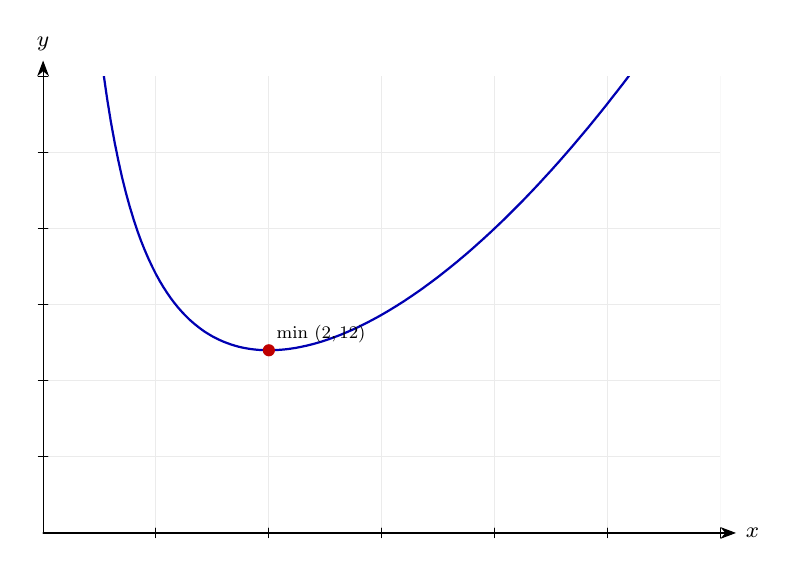
\begin{tikzpicture}[>={Stealth[length=2mm]},font=\footnotesize,line cap=round,line join=round]
\begin{scope}
\clip (0,0) rectangle (8.6,5.8);
\draw[gray!16] (0,0) grid[xstep=1.433,ystep=0.967] (8.6,5.8);
\draw[blue!70!black,thick] (0.048,11.6) -- (0.096,11.6) -- (0.143,11.6) -- (0.191,11.6) -- (0.239,11.6) -- (0.287,11.6) -- (0.334,11.6) -- (0.382,11.6) -- (0.43,10.329) -- (0.478,9.301) -- (0.526,8.462) -- (0.573,7.764) -- (0.621,7.175) -- (0.669,6.671) -- (0.717,6.235) -- (0.764,5.855) -- (0.812,5.521) -- (0.86,5.225) -- (0.908,4.962) -- (0.956,4.726) -- (1.003,4.514) -- (1.051,4.322) -- (1.099,4.148) -- (1.147,3.99) -- (1.194,3.846) -- (1.242,3.714) -- (1.29,3.594) -- (1.338,3.483) -- (1.386,3.381) -- (1.433,3.287) -- (1.481,3.2) -- (1.529,3.12) -- (1.577,3.046) -- (1.624,2.978) -- (1.672,2.915) -- (1.72,2.856) -- (1.768,2.802) -- (1.816,2.752) -- (1.863,2.706) -- (1.911,2.664) -- (1.959,2.625) -- (2.007,2.588) -- (2.054,2.555) -- (2.102,2.525) -- (2.15,2.497) -- (2.198,2.472) -- (2.246,2.449) -- (2.293,2.428) -- (2.341,2.41) -- (2.389,2.393) -- (2.437,2.378) -- (2.484,2.365) -- (2.532,2.354) -- (2.58,2.345) -- (2.628,2.337) -- (2.676,2.331) -- (2.723,2.326) -- (2.771,2.323) -- (2.819,2.321) -- (2.867,2.32) -- (2.914,2.321) -- (2.962,2.323) -- (3.01,2.326) -- (3.058,2.33) -- (3.106,2.335) -- (3.153,2.342) -- (3.201,2.349) -- (3.249,2.358) -- (3.297,2.368) -- (3.344,2.378) -- (3.392,2.39) -- (3.44,2.402) -- (3.488,2.416) -- (3.536,2.43) -- (3.583,2.446) -- (3.631,2.462) -- (3.679,2.479) -- (3.727,2.497) -- (3.774,2.515) -- (3.822,2.535) -- (3.87,2.555) -- (3.918,2.576) -- (3.966,2.598) -- (4.013,2.62) -- (4.061,2.644) -- (4.109,2.668) -- (4.157,2.693) -- (4.204,2.718) -- (4.252,2.744) -- (4.3,2.771) -- (4.348,2.799) -- (4.396,2.827) -- (4.443,2.856) -- (4.491,2.885) -- (4.539,2.916) -- (4.587,2.946) -- (4.634,2.978) -- (4.682,3.01) -- (4.73,3.043) -- (4.778,3.076) -- (4.826,3.11) -- (4.873,3.145) -- (4.921,3.18) -- (4.969,3.216) -- (5.017,3.252) -- (5.064,3.289) -- (5.112,3.327) -- (5.16,3.365) -- (5.208,3.404) -- (5.256,3.443) -- (5.303,3.483) -- (5.351,3.523) -- (5.399,3.564) -- (5.447,3.606) -- (5.494,3.648) -- (5.542,3.691) -- (5.59,3.734) -- (5.638,3.778) -- (5.686,3.822) -- (5.733,3.867) -- (5.781,3.912) -- (5.829,3.958) -- (5.877,4.004) -- (5.924,4.051) -- (5.972,4.099) -- (6.02,4.147) -- (6.068,4.195) -- (6.116,4.245) -- (6.163,4.294) -- (6.211,4.344) -- (6.259,4.395) -- (6.307,4.446) -- (6.354,4.498) -- (6.402,4.55) -- (6.45,4.602) -- (6.498,4.656) -- (6.546,4.709) -- (6.593,4.763) -- (6.641,4.818) -- (6.689,4.873) -- (6.737,4.929) -- (6.784,4.985) -- (6.832,5.042) -- (6.88,5.099) -- (6.928,5.156) -- (6.976,5.215) -- (7.023,5.273) -- (7.071,5.332) -- (7.119,5.392) -- (7.167,5.452) -- (7.214,5.513) -- (7.262,5.574) -- (7.31,5.635) -- (7.358,5.697) -- (7.406,5.76) -- (7.453,5.823) -- (7.501,5.886) -- (7.549,5.95) -- (7.597,6.014) -- (7.644,6.079) -- (7.692,6.145) -- (7.74,6.21) -- (7.788,6.277) -- (7.836,6.344) -- (7.883,6.411) -- (7.931,6.478) -- (7.979,6.547) -- (8.027,6.615) -- (8.074,6.684) -- (8.122,6.754) -- (8.17,6.824) -- (8.218,6.895) -- (8.266,6.966) -- (8.313,7.037) -- (8.361,7.109) -- (8.409,7.181) -- (8.457,7.254) -- (8.504,7.328) -- (8.552,7.401) -- (8.6,7.476);
\end{scope}
\draw[->] (0,0) -- (8.8,0) node[right]{$x$};
\draw[->] (0,0) -- (0,6) node[above]{$y$};
\draw (1.433,-0.06) -- (1.433,0.06);
\draw (2.867,-0.06) -- (2.867,0.06);
\draw (4.3,-0.06) -- (4.3,0.06);
\draw (5.733,-0.06) -- (5.733,0.06);
\draw (7.167,-0.06) -- (7.167,0.06);
\draw (8.6,-0.06) -- (8.6,0.06);
\draw (-0.06,0.967) -- (0.06,0.967);
\draw (-0.06,1.933) -- (0.06,1.933);
\draw (-0.06,2.9) -- (0.06,2.9);
\draw (-0.06,3.867) -- (0.06,3.867);
\draw (-0.06,4.833) -- (0.06,4.833);
\draw (-0.06,5.8) -- (0.06,5.8);
\fill[red!75!black] (2.867,2.32) circle (2.2pt);
\node[above right,scale=0.8] at (2.867,2.32) {min $(2,12)$};
\end{tikzpicture}
}
\end{center}
\small Curve with classified stationary points marked.\normalsize

\medskip\hrule

\section*{Derivatives and Graphs 27\quad\small\texttt{(d4-027)}}
\addcontentsline{toc}{section}{Derivatives and Graphs 27 (d4-027)}
\textit{Difficulty: Foundation \quad\textbar\quad Marks: 6}

\question{Find the stationary points on \( y = 5x^4 - 4x^5 \) and determine their nature.}

\textbf{Worked solution.}

\textit{Step 1: Differentiate.}
\[\begin{gathered}
\frac{\mathrm{d}y}{\mathrm{d}x} = 20x^3 - 20x^4 = 20x^3(1 - x)
\end{gathered}\]
Power rule, then factorise.

\textit{Step 2: Solve \( \dfrac{\mathrm{d}y}{\mathrm{d}x} = 0 \).}
\[\begin{gathered}
20x^3(1-x) = 0 \implies x = 0 \text{ or } x = 1
\end{gathered}\]
Set each factor to zero.

\textit{Step 3: Find \( y \)-coordinates.}
\[\begin{gathered}
y(0) = 0; \quad y(1) = 5 - 4 = 1
\end{gathered}\]
Substitute into the original.

\textit{Step 4: Second derivative.}
\[\begin{gathered}
\frac{\mathrm{d}^2y}{\mathrm{d}x^2} = 60x^2 - 80x^3
\end{gathered}\]
Differentiate the first derivative.

\textit{Step 5: Classify.}
\[\begin{gathered}
x=0: 0 - 0 = 0 \Rightarrow \text{inconclusive - check sign of } \frac{\mathrm{d}y}{\mathrm{d}x} \text{ either side} \newline x=1: 60 - 80 = -20 < 0 \Rightarrow \text{maximum}
\end{gathered}\]
At \( x = 0 \): for \( x < 0 \), \( 20x^3 < 0 \) and \( (1-x) > 0 \), so \( \frac{\mathrm{d}y}{\mathrm{d}x} < 0 \). For small \( x > 0 \), \( 20x^3 > 0 \) and \( (1-x) > 0 \), so \( \frac{\mathrm{d}y}{\mathrm{d}x} > 0 \). Gradient changes from negative to positive $\to$ minimum at \( x = 0 \).

\begin{answerbox}
\textbf{Final answer:}\quad Local minimum at \(\displaystyle  (0, 0) \); local maximum at \(\displaystyle  (1, 1) \)
\end{answerbox}
\textbf{Diagram.}

\begin{center}
\resizebox{\ifdim\width>\linewidth \linewidth\else \width\fi}{!}{%
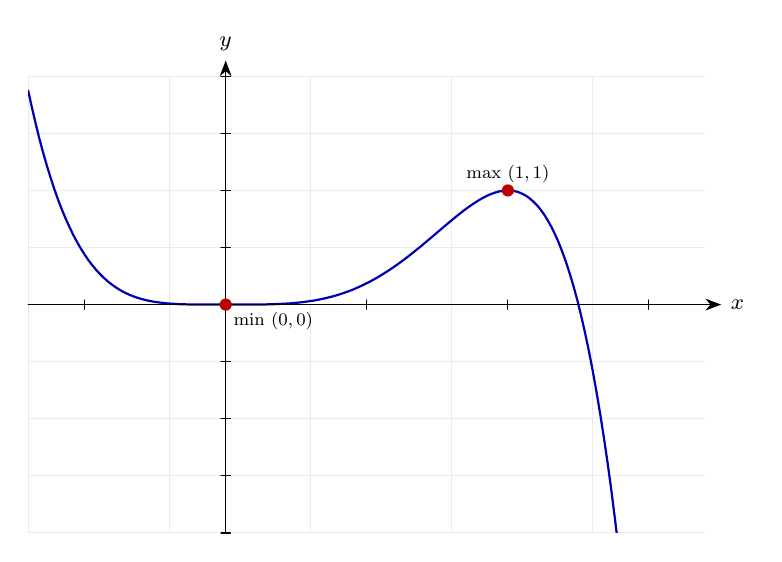
\begin{tikzpicture}[>={Stealth[length=2mm]},font=\footnotesize,line cap=round,line join=round]
\begin{scope}
\clip (0,0) rectangle (8.6,5.8);
\draw[gray!16] (-1.075,0) grid[xstep=1.792,ystep=0.725] (8.6,5.8);
\draw[blue!70!black,thick] (0,5.616) -- (0.048,5.397) -- (0.096,5.193) -- (0.143,5.002) -- (0.191,4.824) -- (0.239,4.657) -- (0.287,4.503) -- (0.334,4.359) -- (0.382,4.225) -- (0.43,4.101) -- (0.478,3.986) -- (0.526,3.881) -- (0.573,3.783) -- (0.621,3.693) -- (0.669,3.61) -- (0.717,3.534) -- (0.764,3.465) -- (0.812,3.402) -- (0.86,3.344) -- (0.908,3.292) -- (0.956,3.244) -- (1.003,3.201) -- (1.051,3.163) -- (1.099,3.128) -- (1.147,3.097) -- (1.194,3.069) -- (1.242,3.045) -- (1.29,3.023) -- (1.338,3.004) -- (1.386,2.987) -- (1.433,2.973) -- (1.481,2.96) -- (1.529,2.949) -- (1.577,2.94) -- (1.624,2.932) -- (1.672,2.926) -- (1.72,2.92) -- (1.768,2.915) -- (1.816,2.912) -- (1.863,2.909) -- (1.911,2.906) -- (1.959,2.904) -- (2.007,2.903) -- (2.054,2.902) -- (2.102,2.901) -- (2.15,2.901) -- (2.198,2.9) -- (2.246,2.9) -- (2.293,2.9) -- (2.341,2.9) -- (2.389,2.9) -- (2.437,2.9) -- (2.484,2.9) -- (2.532,2.9) -- (2.58,2.9) -- (2.628,2.9) -- (2.676,2.9) -- (2.723,2.9) -- (2.771,2.9) -- (2.819,2.9) -- (2.867,2.901) -- (2.914,2.901) -- (2.962,2.902) -- (3.01,2.902) -- (3.058,2.904) -- (3.106,2.905) -- (3.153,2.907) -- (3.201,2.909) -- (3.249,2.911) -- (3.297,2.914) -- (3.344,2.917) -- (3.392,2.922) -- (3.44,2.926) -- (3.488,2.932) -- (3.536,2.938) -- (3.583,2.945) -- (3.631,2.952) -- (3.679,2.961) -- (3.727,2.971) -- (3.774,2.981) -- (3.822,2.993) -- (3.87,3.005) -- (3.918,3.019) -- (3.966,3.034) -- (4.013,3.05) -- (4.061,3.067) -- (4.109,3.085) -- (4.157,3.105) -- (4.204,3.126) -- (4.252,3.148) -- (4.3,3.172) -- (4.348,3.197) -- (4.396,3.223) -- (4.443,3.25) -- (4.491,3.279) -- (4.539,3.309) -- (4.587,3.34) -- (4.634,3.372) -- (4.682,3.405) -- (4.73,3.44) -- (4.778,3.475) -- (4.826,3.512) -- (4.873,3.549) -- (4.921,3.588) -- (4.969,3.626) -- (5.017,3.666) -- (5.064,3.706) -- (5.112,3.746) -- (5.16,3.787) -- (5.208,3.828) -- (5.256,3.869) -- (5.303,3.909) -- (5.351,3.949) -- (5.399,3.989) -- (5.447,4.028) -- (5.494,4.065) -- (5.542,4.102) -- (5.59,4.137) -- (5.638,4.171) -- (5.686,4.202) -- (5.733,4.232) -- (5.781,4.259) -- (5.829,4.283) -- (5.877,4.304) -- (5.924,4.321) -- (5.972,4.335) -- (6.02,4.344) -- (6.068,4.349) -- (6.116,4.349) -- (6.163,4.344) -- (6.211,4.333) -- (6.259,4.315) -- (6.307,4.291) -- (6.354,4.26) -- (6.402,4.221) -- (6.45,4.174) -- (6.498,4.118) -- (6.546,4.053) -- (6.593,3.978) -- (6.641,3.892) -- (6.689,3.795) -- (6.737,3.687) -- (6.784,3.567) -- (6.832,3.433) -- (6.88,3.285) -- (6.928,3.124) -- (6.976,2.947) -- (7.023,2.754) -- (7.071,2.544) -- (7.119,2.317) -- (7.167,2.072) -- (7.214,1.807) -- (7.262,1.523) -- (7.31,1.217) -- (7.358,0.89) -- (7.406,0.539) -- (7.453,0.165) -- (7.501,-0.233) -- (7.549,-0.658) -- (7.597,-1.109) -- (7.644,-1.588) -- (7.692,-2.096) -- (7.74,-2.634) -- (7.788,-3.204) -- (7.836,-3.805) -- (7.883,-4.441) -- (7.931,-5.111) -- (7.979,-5.8) -- (8.027,-5.8) -- (8.074,-5.8) -- (8.122,-5.8) -- (8.17,-5.8) -- (8.218,-5.8) -- (8.266,-5.8) -- (8.313,-5.8) -- (8.361,-5.8) -- (8.409,-5.8) -- (8.457,-5.8) -- (8.504,-5.8) -- (8.552,-5.8) -- (8.6,-5.8);
\end{scope}
\draw[->] (0,2.9) -- (8.8,2.9) node[right]{$x$};
\draw[->] (2.508,0) -- (2.508,6) node[above]{$y$};
\draw (0.717,2.84) -- (0.717,2.96);
\draw (4.3,2.84) -- (4.3,2.96);
\draw (6.092,2.84) -- (6.092,2.96);
\draw (7.883,2.84) -- (7.883,2.96);
\draw (2.448,0) -- (2.568,0);
\draw (2.448,0.725) -- (2.568,0.725);
\draw (2.448,1.45) -- (2.568,1.45);
\draw (2.448,2.175) -- (2.568,2.175);
\draw (2.448,3.625) -- (2.568,3.625);
\draw (2.448,4.35) -- (2.568,4.35);
\draw (2.448,5.075) -- (2.568,5.075);
\draw (2.448,5.8) -- (2.568,5.8);
\fill[red!75!black] (2.508,2.9) circle (2.2pt);
\node[below right,scale=0.8] at (2.508,2.9) {min $(0,0)$};
\fill[red!75!black] (6.092,4.35) circle (2.2pt);
\node[above,scale=0.8] at (6.092,4.35) {max $(1,1)$};
\end{tikzpicture}
}
\end{center}
\small Curve with classified stationary points marked.\normalsize

\medskip\hrule

\section*{Derivatives and Graphs 28\quad\small\texttt{(d4-028)}}
\addcontentsline{toc}{section}{Derivatives and Graphs 28 (d4-028)}
\textit{Difficulty: Foundation \quad\textbar\quad Marks: 4}

\question{Find the range of values of \( x \) for which \( y = x^3 - 6x^2 + 9x + 4 \) is increasing.}

\textbf{Worked solution.}

\textit{Step 1: Differentiate.}
\[\begin{gathered}
\frac{\mathrm{d}y}{\mathrm{d}x} = 3x^2 - 12x + 9
\end{gathered}\]
Power rule.

\textit{Step 2: Solve the inequality \( 3x^2 - 12x + 9 > 0 \).}
\[\begin{gathered}
x^2 - 4x + 3 > 0 \implies (x - 1)(x - 3) > 0
\end{gathered}\]
Divide by 3 and factorise.

\textit{Step 3: Solve.}
\[\begin{gathered}
x < 1 \text{ or } x > 3
\end{gathered}\]
The product is positive outside the roots.

\begin{answerbox}
\textbf{Final answer:}\quad \(\displaystyle  x < 1 \) or \(\displaystyle  x > 3 \)
\end{answerbox}
\textbf{Diagram.}

\begin{center}
\resizebox{\ifdim\width>\linewidth \linewidth\else \width\fi}{!}{%
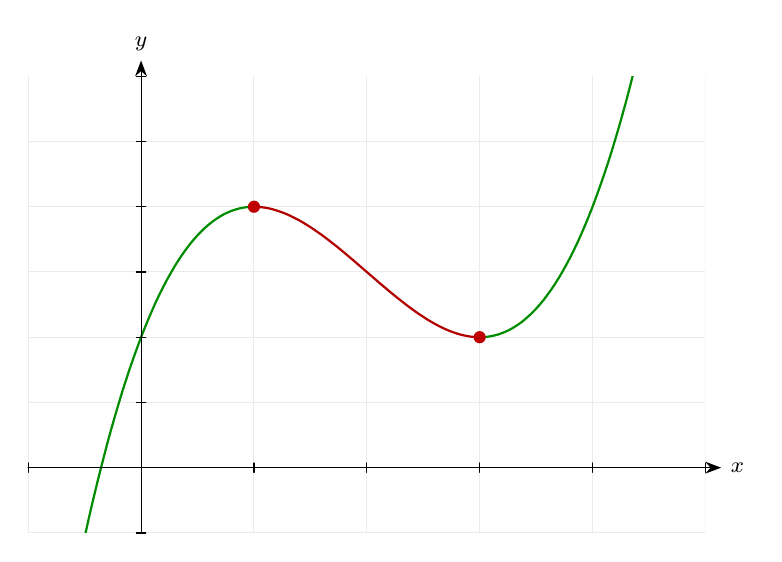
\begin{tikzpicture}[>={Stealth[length=2mm]},font=\footnotesize,line cap=round,line join=round]
\begin{scope}
\clip (0,0) rectangle (8.6,5.8);
\draw[gray!16] (0,0) grid[xstep=1.433,ystep=0.829] (8.6,5.8);
\draw[green!55!black,thick] (0,-4.143) -- (0.048,-3.816) -- (0.096,-3.496) -- (0.143,-3.185) -- (0.191,-2.882) -- (0.239,-2.587) -- (0.287,-2.3) -- (0.334,-2.021) -- (0.382,-1.749) -- (0.43,-1.484) -- (0.478,-1.228) -- (0.526,-0.978) -- (0.573,-0.736) -- (0.621,-0.501) -- (0.669,-0.273) -- (0.717,-0.052) -- (0.764,0.162) -- (0.812,0.37) -- (0.86,0.57) -- (0.908,0.764) -- (0.956,0.951) -- (1.003,1.132) -- (1.051,1.307) -- (1.099,1.475) -- (1.147,1.637) -- (1.194,1.793) -- (1.242,1.943) -- (1.29,2.088) -- (1.338,2.226) -- (1.386,2.359) -- (1.433,2.486) -- (1.481,2.607) -- (1.529,2.723) -- (1.577,2.834) -- (1.624,2.94) -- (1.672,3.04) -- (1.72,3.135) -- (1.768,3.226) -- (1.816,3.311) -- (1.863,3.392) -- (1.911,3.468) -- (1.959,3.539) -- (2.007,3.606) -- (2.054,3.668) -- (2.102,3.726) -- (2.15,3.78) -- (2.198,3.83) -- (2.246,3.876) -- (2.293,3.917) -- (2.341,3.955) -- (2.389,3.989) -- (2.437,4.02) -- (2.484,4.047) -- (2.532,4.07) -- (2.58,4.09) -- (2.628,4.106) -- (2.676,4.12) -- (2.723,4.13) -- (2.771,4.137) -- (2.819,4.141) -- (2.867,4.143);
\draw[red!70!black,thick] (2.867,4.143) -- (2.914,4.141) -- (2.962,4.137) -- (3.01,4.131) -- (3.058,4.122) -- (3.106,4.11) -- (3.153,4.096) -- (3.201,4.08) -- (3.249,4.062) -- (3.297,4.042) -- (3.344,4.02) -- (3.392,3.996) -- (3.44,3.971) -- (3.488,3.943) -- (3.536,3.914) -- (3.583,3.884) -- (3.631,3.852) -- (3.679,3.819) -- (3.727,3.785) -- (3.774,3.75) -- (3.822,3.713) -- (3.87,3.676) -- (3.918,3.638) -- (3.966,3.599) -- (4.013,3.56) -- (4.061,3.52) -- (4.109,3.479) -- (4.157,3.438) -- (4.204,3.397) -- (4.252,3.356) -- (4.3,3.314) -- (4.348,3.273) -- (4.396,3.232) -- (4.443,3.19) -- (4.491,3.15) -- (4.539,3.109) -- (4.587,3.069) -- (4.634,3.03) -- (4.682,2.991) -- (4.73,2.953) -- (4.778,2.915) -- (4.826,2.879) -- (4.873,2.844) -- (4.921,2.809) -- (4.969,2.776) -- (5.017,2.745) -- (5.064,2.714) -- (5.112,2.685) -- (5.16,2.658) -- (5.208,2.632) -- (5.256,2.608) -- (5.303,2.586) -- (5.351,2.566) -- (5.399,2.548) -- (5.447,2.532) -- (5.494,2.518) -- (5.542,2.507) -- (5.59,2.498) -- (5.638,2.491) -- (5.686,2.487) -- (5.733,2.486);
\draw[green!55!black,thick] (5.733,2.486) -- (5.781,2.487) -- (5.829,2.491) -- (5.877,2.499) -- (5.924,2.509) -- (5.972,2.522) -- (6.02,2.539) -- (6.068,2.559) -- (6.116,2.582) -- (6.163,2.609) -- (6.211,2.639) -- (6.259,2.673) -- (6.307,2.711) -- (6.354,2.753) -- (6.402,2.798) -- (6.45,2.848) -- (6.498,2.902) -- (6.546,2.96) -- (6.593,3.023) -- (6.641,3.089) -- (6.689,3.161) -- (6.737,3.237) -- (6.784,3.317) -- (6.832,3.403) -- (6.88,3.493) -- (6.928,3.589) -- (6.976,3.689) -- (7.023,3.794) -- (7.071,3.905) -- (7.119,4.021) -- (7.167,4.143) -- (7.214,4.27) -- (7.262,4.403) -- (7.31,4.541) -- (7.358,4.685) -- (7.406,4.835) -- (7.453,4.991) -- (7.501,5.153) -- (7.549,5.322) -- (7.597,5.496) -- (7.644,5.677) -- (7.692,5.865) -- (7.74,6.059) -- (7.788,6.259) -- (7.836,6.466) -- (7.883,6.68) -- (7.931,6.901) -- (7.979,7.129) -- (8.027,7.364) -- (8.074,7.607) -- (8.122,7.856) -- (8.17,8.113) -- (8.218,8.377) -- (8.266,8.649) -- (8.313,8.929) -- (8.361,9.216) -- (8.409,9.511) -- (8.457,9.814) -- (8.504,10.125) -- (8.552,10.444) -- (8.6,10.771);
\end{scope}
\draw[->] (0,0.829) -- (8.8,0.829) node[right]{$x$};
\draw[->] (1.433,0) -- (1.433,6) node[above]{$y$};
\draw (0,0.769) -- (0,0.889);
\draw (2.867,0.769) -- (2.867,0.889);
\draw (4.3,0.769) -- (4.3,0.889);
\draw (5.733,0.769) -- (5.733,0.889);
\draw (7.167,0.769) -- (7.167,0.889);
\draw (8.6,0.769) -- (8.6,0.889);
\draw (1.373,0) -- (1.493,0);
\draw (1.373,1.657) -- (1.493,1.657);
\draw (1.373,2.486) -- (1.493,2.486);
\draw (1.373,3.314) -- (1.493,3.314);
\draw (1.373,4.143) -- (1.493,4.143);
\draw (1.373,4.971) -- (1.493,4.971);
\draw (1.373,5.8) -- (1.493,5.8);
\fill[red!75!black] (2.867,4.143) circle (2.2pt);
\fill[red!75!black] (5.733,2.486) circle (2.2pt);
\end{tikzpicture}
}
\end{center}
\small Curve coloured green where increasing, red where decreasing.\normalsize

\medskip\hrule

\section*{Derivatives and Graphs 29\quad\small\texttt{(d4-029)}}
\addcontentsline{toc}{section}{Derivatives and Graphs 29 (d4-029)}
\textit{Difficulty: Foundation \quad\textbar\quad Marks: 7}

\question{A curve has equation \( y = x^3 - 3x + 2 \). (a) Find the \( x \)-intercepts. (b) Find and classify the stationary points. (c) Describe the shape of a sketch of the curve.}

\textbf{Worked solution.}

\textit{Step 1: (a) Solve \( x^3 - 3x + 2 = 0 \).}
\[\begin{gathered}
x = 1 \text{ is a root: } (x-1)(x^2 + x - 2) = (x-1)(x-1)(x+2) = (x-1)^2(x+2)
\end{gathered}\]
Try \( x = 1 \), then factorise the quotient \( x^2 + x - 2 \).

\textit{Step 2: \( x \)-intercepts.}
\[\begin{gathered}
x = 1 \text{ (double root)}, \; x = -2
\end{gathered}\]
\( (x-1)^2(x+2)=0 \). Double root at \(x=1\) means the curve touches the axis there.

\textit{Step 3: (b) Differentiate.}
\[\begin{gathered}
\frac{\mathrm{d}y}{\mathrm{d}x} = 3x^2 - 3 = 3(x-1)(x+1)
\end{gathered}\]
Set to zero: \( x = 1 \) or \( x = -1 \).

\textit{Step 4: Coordinates.}
\[\begin{gathered}
x=1: y = 1-3+2=0; \quad x=-1: y = -1+3+2=4
\end{gathered}\]
Substitute into the original.

\textit{Step 5: Classify.}
\[\begin{gathered}
\frac{\mathrm{d}^2y}{\mathrm{d}x^2} = 6x \newline x=1: 6>0 \Rightarrow \text{minimum} \newline x=-1: -6<0 \Rightarrow \text{maximum}
\end{gathered}\]
Second derivative test.

\textit{Step 6: (c) Sketch description.}
\[\begin{gathered}
\text{Positive cubic; crosses at }(-2,0)\text{; touches at }(1,0)\text{; local max at }(-1,4)\text{; local min at }(1,0).
\end{gathered}\]
The curve enters from bottom-left, rises to a local max at \((-1,4)\), dips to touch the axis at \((1,0)\), then rises to top-right.

\begin{answerbox}
\textbf{Final answer:}\quad (a) \(\displaystyle  x = -2 \) and \(\displaystyle  x = 1 \) (double root) \\[3pt]  (b) Local maximum at \(\displaystyle  (-1, 4) \); local minimum at \(\displaystyle  (1, 0) \) \\[3pt]  (c) Positive cubic; touches \(\displaystyle  x \)-axis at \(\displaystyle  (1,0) \)
\end{answerbox}
\textbf{Diagram.}

\begin{center}
\resizebox{\ifdim\width>\linewidth \linewidth\else \width\fi}{!}{%
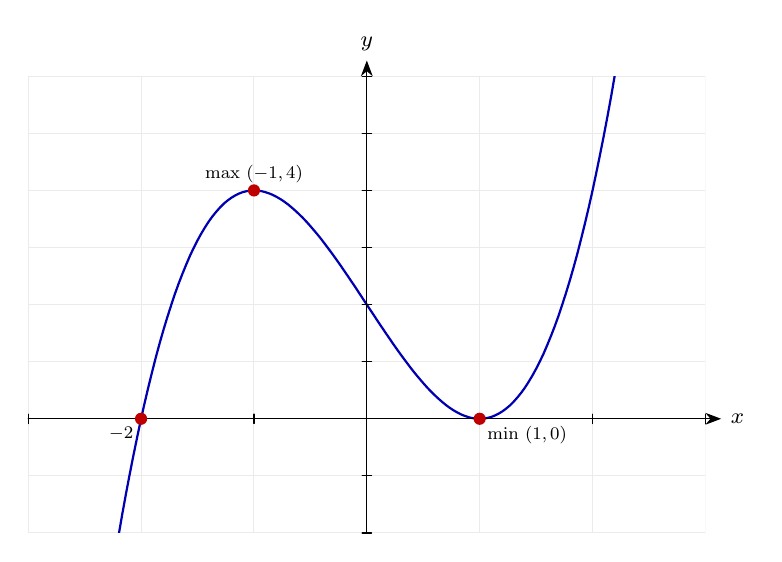
\begin{tikzpicture}[>={Stealth[length=2mm]},font=\footnotesize,line cap=round,line join=round]
\begin{scope}
\clip (0,0) rectangle (8.6,5.8);
\draw[gray!16] (0,0) grid[xstep=1.433,ystep=0.725] (8.6,5.8);
\draw[blue!70!black,thick] (0,-5.8) -- (0.048,-5.8) -- (0.096,-5.8) -- (0.143,-5.8) -- (0.191,-5.8) -- (0.239,-5.8) -- (0.287,-5.8) -- (0.334,-5.8) -- (0.382,-5.8) -- (0.43,-5.498) -- (0.478,-5.048) -- (0.526,-4.612) -- (0.573,-4.188) -- (0.621,-3.776) -- (0.669,-3.377) -- (0.717,-2.991) -- (0.764,-2.616) -- (0.812,-2.253) -- (0.86,-1.902) -- (0.908,-1.563) -- (0.956,-1.235) -- (1.003,-0.919) -- (1.051,-0.613) -- (1.099,-0.319) -- (1.147,-0.035) -- (1.194,0.238) -- (1.242,0.501) -- (1.29,0.753) -- (1.338,0.995) -- (1.386,1.228) -- (1.433,1.45) -- (1.481,1.663) -- (1.529,1.866) -- (1.577,2.06) -- (1.624,2.244) -- (1.672,2.42) -- (1.72,2.587) -- (1.768,2.745) -- (1.816,2.894) -- (1.863,3.036) -- (1.911,3.169) -- (1.959,3.293) -- (2.007,3.41) -- (2.054,3.52) -- (2.102,3.621) -- (2.15,3.716) -- (2.198,3.803) -- (2.246,3.883) -- (2.293,3.956) -- (2.341,4.022) -- (2.389,4.081) -- (2.437,4.135) -- (2.484,4.182) -- (2.532,4.222) -- (2.58,4.257) -- (2.628,4.286) -- (2.676,4.31) -- (2.723,4.328) -- (2.771,4.34) -- (2.819,4.348) -- (2.867,4.35) -- (2.914,4.348) -- (2.962,4.341) -- (3.01,4.329) -- (3.058,4.313) -- (3.106,4.293) -- (3.153,4.269) -- (3.201,4.241) -- (3.249,4.209) -- (3.297,4.174) -- (3.344,4.135) -- (3.392,4.093) -- (3.44,4.048) -- (3.488,4.001) -- (3.536,3.95) -- (3.583,3.897) -- (3.631,3.841) -- (3.679,3.784) -- (3.727,3.724) -- (3.774,3.662) -- (3.822,3.598) -- (3.87,3.533) -- (3.918,3.466) -- (3.966,3.398) -- (4.013,3.329) -- (4.061,3.259) -- (4.109,3.188) -- (4.157,3.117) -- (4.204,3.045) -- (4.252,2.972) -- (4.3,2.9) -- (4.348,2.828) -- (4.396,2.755) -- (4.443,2.683) -- (4.491,2.612) -- (4.539,2.541) -- (4.587,2.471) -- (4.634,2.402) -- (4.682,2.334) -- (4.73,2.267) -- (4.778,2.202) -- (4.826,2.138) -- (4.873,2.076) -- (4.921,2.016) -- (4.969,1.959) -- (5.017,1.903) -- (5.064,1.85) -- (5.112,1.799) -- (5.16,1.752) -- (5.208,1.707) -- (5.256,1.665) -- (5.303,1.626) -- (5.351,1.591) -- (5.399,1.559) -- (5.447,1.531) -- (5.494,1.507) -- (5.542,1.487) -- (5.59,1.471) -- (5.638,1.459) -- (5.686,1.452) -- (5.733,1.45) -- (5.781,1.452) -- (5.829,1.46) -- (5.877,1.472) -- (5.924,1.49) -- (5.972,1.514) -- (6.02,1.543) -- (6.068,1.578) -- (6.116,1.618) -- (6.163,1.665) -- (6.211,1.719) -- (6.259,1.778) -- (6.307,1.844) -- (6.354,1.917) -- (6.402,1.997) -- (6.45,2.084) -- (6.498,2.179) -- (6.546,2.28) -- (6.593,2.39) -- (6.641,2.507) -- (6.689,2.631) -- (6.737,2.764) -- (6.784,2.906) -- (6.832,3.055) -- (6.88,3.213) -- (6.928,3.38) -- (6.976,3.556) -- (7.023,3.74) -- (7.071,3.934) -- (7.119,4.137) -- (7.167,4.35) -- (7.214,4.572) -- (7.262,4.805) -- (7.31,5.047) -- (7.358,5.299) -- (7.406,5.562) -- (7.453,5.835) -- (7.501,6.119) -- (7.549,6.413) -- (7.597,6.719) -- (7.644,7.035) -- (7.692,7.363) -- (7.74,7.702) -- (7.788,8.053) -- (7.836,8.416) -- (7.883,8.791) -- (7.931,9.177) -- (7.979,9.576) -- (8.027,9.988) -- (8.074,10.412) -- (8.122,10.848) -- (8.17,11.298) -- (8.218,11.6) -- (8.266,11.6) -- (8.313,11.6) -- (8.361,11.6) -- (8.409,11.6) -- (8.457,11.6) -- (8.504,11.6) -- (8.552,11.6) -- (8.6,11.6);
\end{scope}
\draw[->] (0,1.45) -- (8.8,1.45) node[right]{$x$};
\draw[->] (4.3,0) -- (4.3,6) node[above]{$y$};
\draw (0,1.39) -- (0,1.51);
\draw (1.433,1.39) -- (1.433,1.51);
\draw (2.867,1.39) -- (2.867,1.51);
\draw (5.733,1.39) -- (5.733,1.51);
\draw (7.167,1.39) -- (7.167,1.51);
\draw (8.6,1.39) -- (8.6,1.51);
\draw (4.24,0) -- (4.36,0);
\draw (4.24,0.725) -- (4.36,0.725);
\draw (4.24,2.175) -- (4.36,2.175);
\draw (4.24,2.9) -- (4.36,2.9);
\draw (4.24,3.625) -- (4.36,3.625);
\draw (4.24,4.35) -- (4.36,4.35);
\draw (4.24,5.075) -- (4.36,5.075);
\draw (4.24,5.8) -- (4.36,5.8);
\fill[red!75!black] (2.867,4.35) circle (2.2pt);
\node[above,scale=0.8] at (2.867,4.35) {max $(-1,4)$};
\fill[red!75!black] (5.733,1.45) circle (2.2pt);
\node[below right,scale=0.8] at (5.733,1.45) {min $(1,0)$};
\fill[red!75!black] (1.433,1.45) circle (2.2pt);
\node[below left,scale=0.8] at (1.433,1.45) {$-2$};
\end{tikzpicture}
}
\end{center}
\small Curve with classified stationary points marked.\normalsize

\medskip\hrule

\section*{Derivatives and Graphs 30\quad\small\texttt{(d4-030)}}
\addcontentsline{toc}{section}{Derivatives and Graphs 30 (d4-030)}
\textit{Difficulty: Foundation \quad\textbar\quad Marks: 4}

\question{The function \( y = 5 - 3x - ax^2 \) is a decreasing function for all real values of \( x \). Find the range of possible values of \( a \).}

\textbf{Worked solution.}

\textit{Step 1: Differentiate.}
\[\begin{gathered}
\frac{\mathrm{d}y}{\mathrm{d}x} = -3 - 2ax
\end{gathered}\]
Power rule.

\textit{Step 2: For the function to be decreasing for all \( x \), we need \( \dfrac{\mathrm{d}y}{\mathrm{d}x} \leq 0 \) for all \( x \).}
\[\begin{gathered}
-3 - 2ax \leq 0 \text{ for all } x
\end{gathered}\]
This must hold for every real \( x \), not just at a specific point.

\textit{Step 3: The derivative \( -3 - 2ax \) is linear in \( x \). A non-constant linear function takes both signs, so for \( \dfrac{\mathrm{d}y}{\mathrm{d}x} \leq 0 \) to hold for every real \( x \), the coefficient of \( x \) must vanish.}
\[\begin{gathered}
-2a = 0 \implies a = 0
\end{gathered}\]
If \( a \neq 0 \) the gradient \( -3 - 2ax \) is positive for large \( |x| \) of the appropriate sign, so the curve is not decreasing everywhere. Setting the coefficient of \( x \) to zero is the only way to force the gradient to be the constant \(-3\).

\textit{Step 4: Check the constant term is negative.}
\[\begin{gathered}
a = 0 \Rightarrow \dfrac{\mathrm{d}y}{\mathrm{d}x} = -3 < 0 \checkmark
\end{gathered}\]
With \( a = 0 \), the function reduces to \( y = 5 - 3x \), a straight line with constant negative gradient --- decreasing for every real \( x \).

\begin{answerbox}
\textbf{Final answer:}\quad \(\displaystyle  a = 0 \) (for the function to be strictly decreasing for all real \(\displaystyle  x \))
\end{answerbox}
\textbf{Diagram.}

\begin{center}
\resizebox{\ifdim\width>\linewidth \linewidth\else \width\fi}{!}{%
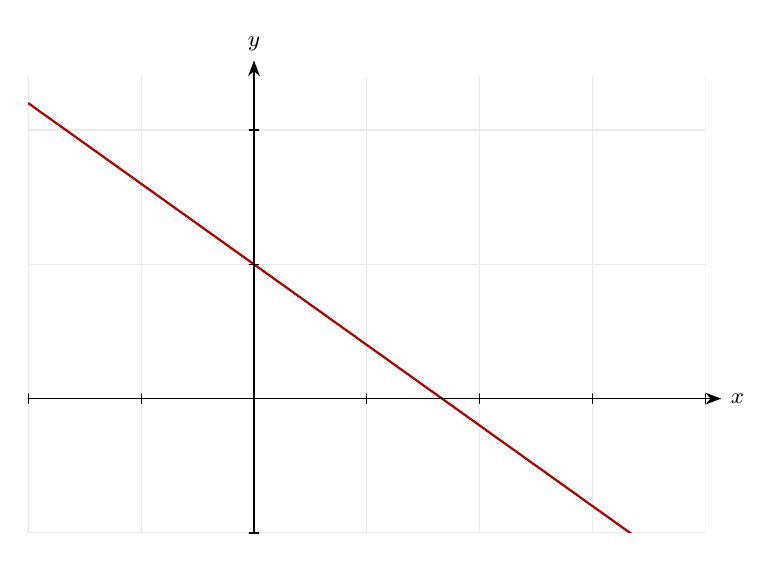
\begin{tikzpicture}[>={Stealth[length=2mm]},font=\footnotesize,line cap=round,line join=round]
\begin{scope}
\clip (0,0) rectangle (8.6,5.8);
\draw[gray!16] (0,0) grid[xstep=1.433,ystep=1.706] (8.6,5.8);
\draw[red!70!black,thick] (0,5.459) -- (0.048,5.425) -- (0.096,5.391) -- (0.143,5.356) -- (0.191,5.322) -- (0.239,5.288) -- (0.287,5.254) -- (0.334,5.22) -- (0.382,5.186) -- (0.43,5.152) -- (0.478,5.118) -- (0.526,5.084) -- (0.573,5.049) -- (0.621,5.015) -- (0.669,4.981) -- (0.717,4.947) -- (0.764,4.913) -- (0.812,4.879) -- (0.86,4.845) -- (0.908,4.811) -- (0.956,4.776) -- (1.003,4.742) -- (1.051,4.708) -- (1.099,4.674) -- (1.147,4.64) -- (1.194,4.606) -- (1.242,4.572) -- (1.29,4.538) -- (1.338,4.504) -- (1.386,4.469) -- (1.433,4.435) -- (1.481,4.401) -- (1.529,4.367) -- (1.577,4.333) -- (1.624,4.299) -- (1.672,4.265) -- (1.72,4.231) -- (1.768,4.196) -- (1.816,4.162) -- (1.863,4.128) -- (1.911,4.094) -- (1.959,4.06) -- (2.007,4.026) -- (2.054,3.992) -- (2.102,3.958) -- (2.15,3.924) -- (2.198,3.889) -- (2.246,3.855) -- (2.293,3.821) -- (2.341,3.787) -- (2.389,3.753) -- (2.437,3.719) -- (2.484,3.685) -- (2.532,3.651) -- (2.58,3.616) -- (2.628,3.582) -- (2.676,3.548) -- (2.723,3.514) -- (2.771,3.48) -- (2.819,3.446) -- (2.867,3.412) -- (2.914,3.378) -- (2.962,3.344) -- (3.01,3.309) -- (3.058,3.275) -- (3.106,3.241) -- (3.153,3.207) -- (3.201,3.173) -- (3.249,3.139) -- (3.297,3.105) -- (3.344,3.071) -- (3.392,3.036) -- (3.44,3.002) -- (3.488,2.968) -- (3.536,2.934) -- (3.583,2.9) -- (3.631,2.866) -- (3.679,2.832) -- (3.727,2.798) -- (3.774,2.764) -- (3.822,2.729) -- (3.87,2.695) -- (3.918,2.661) -- (3.966,2.627) -- (4.013,2.593) -- (4.061,2.559) -- (4.109,2.525) -- (4.157,2.491) -- (4.204,2.456) -- (4.252,2.422) -- (4.3,2.388) -- (4.348,2.354) -- (4.396,2.32) -- (4.443,2.286) -- (4.491,2.252) -- (4.539,2.218) -- (4.587,2.184) -- (4.634,2.149) -- (4.682,2.115) -- (4.73,2.081) -- (4.778,2.047) -- (4.826,2.013) -- (4.873,1.979) -- (4.921,1.945) -- (4.969,1.911) -- (5.017,1.876) -- (5.064,1.842) -- (5.112,1.808) -- (5.16,1.774) -- (5.208,1.74) -- (5.256,1.706) -- (5.303,1.672) -- (5.351,1.638) -- (5.399,1.604) -- (5.447,1.569) -- (5.494,1.535) -- (5.542,1.501) -- (5.59,1.467) -- (5.638,1.433) -- (5.686,1.399) -- (5.733,1.365) -- (5.781,1.331) -- (5.829,1.296) -- (5.877,1.262) -- (5.924,1.228) -- (5.972,1.194) -- (6.02,1.16) -- (6.068,1.126) -- (6.116,1.092) -- (6.163,1.058) -- (6.211,1.024) -- (6.259,0.989) -- (6.307,0.955) -- (6.354,0.921) -- (6.402,0.887) -- (6.45,0.853) -- (6.498,0.819) -- (6.546,0.785) -- (6.593,0.751) -- (6.641,0.716) -- (6.689,0.682) -- (6.737,0.648) -- (6.784,0.614) -- (6.832,0.58) -- (6.88,0.546) -- (6.928,0.512) -- (6.976,0.478) -- (7.023,0.444) -- (7.071,0.409) -- (7.119,0.375) -- (7.167,0.341) -- (7.214,0.307) -- (7.262,0.273) -- (7.31,0.239) -- (7.358,0.205) -- (7.406,0.171) -- (7.453,0.136) -- (7.501,0.102) -- (7.549,0.068) -- (7.597,0.034) -- (7.644,0) -- (7.692,-0.034) -- (7.74,-0.068) -- (7.788,-0.102) -- (7.836,-0.136) -- (7.883,-0.171) -- (7.931,-0.205) -- (7.979,-0.239) -- (8.027,-0.273) -- (8.074,-0.307) -- (8.122,-0.341) -- (8.17,-0.375) -- (8.218,-0.409) -- (8.266,-0.444) -- (8.313,-0.478) -- (8.361,-0.512) -- (8.409,-0.546) -- (8.457,-0.58) -- (8.504,-0.614) -- (8.552,-0.648) -- (8.6,-0.682);
\end{scope}
\draw[->] (0,1.706) -- (8.8,1.706) node[right]{$x$};
\draw[->] (2.867,0) -- (2.867,6) node[above]{$y$};
\draw (0,1.646) -- (0,1.766);
\draw (1.433,1.646) -- (1.433,1.766);
\draw (4.3,1.646) -- (4.3,1.766);
\draw (5.733,1.646) -- (5.733,1.766);
\draw (7.167,1.646) -- (7.167,1.766);
\draw (8.6,1.646) -- (8.6,1.766);
\draw (2.807,0) -- (2.927,0);
\draw (2.807,3.412) -- (2.927,3.412);
\draw (2.807,5.118) -- (2.927,5.118);
\end{tikzpicture}
}
\end{center}
\small Curve coloured green where increasing, red where decreasing.\normalsize

\medskip\hrule

\section*{Derivatives and Graphs 31\quad\small\texttt{(d4-031)}}
\addcontentsline{toc}{section}{Derivatives and Graphs 31 (d4-031)}
\textit{Difficulty: Foundation \quad\textbar\quad Marks: 9}

\question{The curve \( C \) has equation \( y = f(x) \) where \( f(x) = x^3 - 6x^2 + 9x - 2 \). (a) Find \( f'(x) \). (b) Find the coordinates of the stationary points of \( C \). (c) Determine the nature of each stationary point. (d) Find the range of values of \( x \) for which \( f(x) \) is increasing.}

\textbf{Worked solution.}

\textit{Step 1: (a) Differentiate.}
\[\begin{gathered}
f'(x) = 3x^2 - 12x + 9
\end{gathered}\]
Power rule.

\textit{Step 2: (b) Solve \( f'(x) = 0 \).}
\[\begin{gathered}
3x^2 - 12x + 9 = 0 \implies x^2 - 4x + 3 = 0 \implies (x-1)(x-3) = 0
\end{gathered}\]
Divide by 3 and factorise.

\textit{Step 3: Coordinates.}
\[\begin{gathered}
f(1) = 1 - 6 + 9 - 2 = 2; \quad f(3) = 27 - 54 + 27 - 2 = -2
\end{gathered}\]
Substitute each \( x \) into \( f(x) \).

\textit{Step 4: (c) Second derivative.}
\[\begin{gathered}
f''(x) = 6x - 12 \newline f''(1) = -6 < 0 \Rightarrow \text{maximum} \newline f''(3) = 6 > 0 \Rightarrow \text{minimum}
\end{gathered}\]
Apply the second derivative test.

\textit{Step 5: (d) Increasing: \( f'(x) > 0 \).}
\[\begin{gathered}
(x-1)(x-3) > 0 \implies x < 1 \text{ or } x > 3
\end{gathered}\]
The factorised form of \( f'(x) \) makes solving the inequality straightforward.

\begin{answerbox}
\textbf{Final answer:}\quad (a) \(\displaystyle  f'(x) = 3x^2-12x+9 \) \\[3pt]  (b) \(\displaystyle  (1, 2) \) and \(\displaystyle  (3, -2) \) \\[3pt]  (c) Local maximum at \(\displaystyle  (1, 2) \); local minimum at \(\displaystyle  (3, -2) \) \\[3pt]  (d) \(\displaystyle  x < 1 \) or \(\displaystyle  x > 3 \)
\end{answerbox}
\textbf{Diagram.}

\begin{center}
\resizebox{\ifdim\width>\linewidth \linewidth\else \width\fi}{!}{%
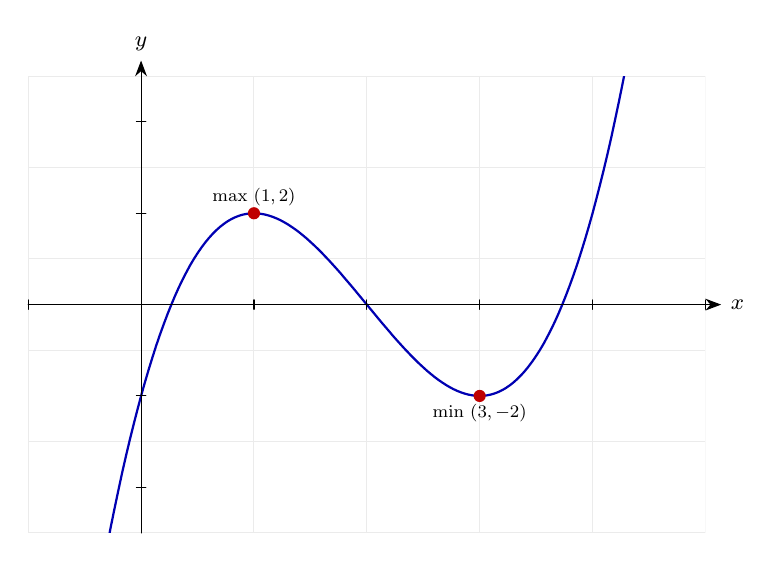
\begin{tikzpicture}[>={Stealth[length=2mm]},font=\footnotesize,line cap=round,line join=round]
\begin{scope}
\clip (0,0) rectangle (8.6,5.8);
\draw[gray!16] (0,-0.58) grid[xstep=1.433,ystep=1.16] (8.6,5.8);
\draw[blue!70!black,thick] (0,-5.8) -- (0.048,-5.8) -- (0.096,-5.8) -- (0.143,-5.8) -- (0.191,-5.775) -- (0.239,-5.362) -- (0.287,-4.96) -- (0.334,-4.569) -- (0.382,-4.188) -- (0.43,-3.818) -- (0.478,-3.459) -- (0.526,-3.109) -- (0.573,-2.77) -- (0.621,-2.441) -- (0.669,-2.122) -- (0.717,-1.812) -- (0.764,-1.513) -- (0.812,-1.223) -- (0.86,-0.942) -- (0.908,-0.67) -- (0.956,-0.408) -- (1.003,-0.155) -- (1.051,0.09) -- (1.099,0.325) -- (1.147,0.552) -- (1.194,0.771) -- (1.242,0.981) -- (1.29,1.183) -- (1.338,1.376) -- (1.386,1.562) -- (1.433,1.74) -- (1.481,1.91) -- (1.529,2.073) -- (1.577,2.228) -- (1.624,2.376) -- (1.672,2.516) -- (1.72,2.649) -- (1.768,2.776) -- (1.816,2.896) -- (1.863,3.008) -- (1.911,3.115) -- (1.959,3.215) -- (2.007,3.308) -- (2.054,3.396) -- (2.102,3.477) -- (2.15,3.552) -- (2.198,3.622) -- (2.246,3.686) -- (2.293,3.744) -- (2.341,3.797) -- (2.389,3.845) -- (2.437,3.888) -- (2.484,3.925) -- (2.532,3.958) -- (2.58,3.986) -- (2.628,4.009) -- (2.676,4.028) -- (2.723,4.042) -- (2.771,4.052) -- (2.819,4.058) -- (2.867,4.06) -- (2.914,4.058) -- (2.962,4.052) -- (3.01,4.043) -- (3.058,4.03) -- (3.106,4.014) -- (3.153,3.995) -- (3.201,3.973) -- (3.249,3.947) -- (3.297,3.919) -- (3.344,3.888) -- (3.392,3.855) -- (3.44,3.819) -- (3.488,3.78) -- (3.536,3.74) -- (3.583,3.697) -- (3.631,3.653) -- (3.679,3.607) -- (3.727,3.559) -- (3.774,3.509) -- (3.822,3.459) -- (3.87,3.406) -- (3.918,3.353) -- (3.966,3.299) -- (4.013,3.243) -- (4.061,3.187) -- (4.109,3.131) -- (4.157,3.073) -- (4.204,3.016) -- (4.252,2.958) -- (4.3,2.9) -- (4.348,2.842) -- (4.396,2.784) -- (4.443,2.727) -- (4.491,2.669) -- (4.539,2.613) -- (4.587,2.557) -- (4.634,2.501) -- (4.682,2.447) -- (4.73,2.394) -- (4.778,2.341) -- (4.826,2.291) -- (4.873,2.241) -- (4.921,2.193) -- (4.969,2.147) -- (5.017,2.103) -- (5.064,2.06) -- (5.112,2.02) -- (5.16,1.981) -- (5.208,1.945) -- (5.256,1.912) -- (5.303,1.881) -- (5.351,1.853) -- (5.399,1.827) -- (5.447,1.805) -- (5.494,1.786) -- (5.542,1.77) -- (5.59,1.757) -- (5.638,1.748) -- (5.686,1.742) -- (5.733,1.74) -- (5.781,1.742) -- (5.829,1.748) -- (5.877,1.758) -- (5.924,1.772) -- (5.972,1.791) -- (6.02,1.814) -- (6.068,1.842) -- (6.116,1.875) -- (6.163,1.912) -- (6.211,1.955) -- (6.259,2.003) -- (6.307,2.056) -- (6.354,2.114) -- (6.402,2.178) -- (6.45,2.248) -- (6.498,2.323) -- (6.546,2.404) -- (6.593,2.492) -- (6.641,2.585) -- (6.689,2.685) -- (6.737,2.792) -- (6.784,2.904) -- (6.832,3.024) -- (6.88,3.151) -- (6.928,3.284) -- (6.976,3.424) -- (7.023,3.572) -- (7.071,3.727) -- (7.119,3.89) -- (7.167,4.06) -- (7.214,4.238) -- (7.262,4.424) -- (7.31,4.617) -- (7.358,4.819) -- (7.406,5.029) -- (7.453,5.248) -- (7.501,5.475) -- (7.549,5.71) -- (7.597,5.955) -- (7.644,6.208) -- (7.692,6.47) -- (7.74,6.742) -- (7.788,7.023) -- (7.836,7.313) -- (7.883,7.612) -- (7.931,7.922) -- (7.979,8.241) -- (8.027,8.57) -- (8.074,8.909) -- (8.122,9.259) -- (8.17,9.618) -- (8.218,9.988) -- (8.266,10.369) -- (8.313,10.76) -- (8.361,11.162) -- (8.409,11.575) -- (8.457,11.6) -- (8.504,11.6) -- (8.552,11.6) -- (8.6,11.6);
\end{scope}
\draw[->] (0,2.9) -- (8.8,2.9) node[right]{$x$};
\draw[->] (1.433,0) -- (1.433,6) node[above]{$y$};
\draw (0,2.84) -- (0,2.96);
\draw (2.867,2.84) -- (2.867,2.96);
\draw (4.3,2.84) -- (4.3,2.96);
\draw (5.733,2.84) -- (5.733,2.96);
\draw (7.167,2.84) -- (7.167,2.96);
\draw (8.6,2.84) -- (8.6,2.96);
\draw (1.373,0.58) -- (1.493,0.58);
\draw (1.373,1.74) -- (1.493,1.74);
\draw (1.373,4.06) -- (1.493,4.06);
\draw (1.373,5.22) -- (1.493,5.22);
\fill[red!75!black] (2.867,4.06) circle (2.2pt);
\node[above,scale=0.8] at (2.867,4.06) {max $(1,2)$};
\fill[red!75!black] (5.733,1.74) circle (2.2pt);
\node[below,scale=0.8] at (5.733,1.74) {min $(3,-2)$};
\end{tikzpicture}
}
\end{center}
\small Curve with classified stationary points marked.\normalsize

\medskip\hrule

\section*{Derivatives and Graphs 32\quad\small\texttt{(d4-032)}}
\addcontentsline{toc}{section}{Derivatives and Graphs 32 (d4-032)}
\textit{Difficulty: Foundation \quad\textbar\quad Marks: 7}

\question{Sketch the graph of \( y = x^3 + 6x^2 + 9x \), clearly labelling all axis intercepts and stationary points with their coordinates.}

\textbf{Worked solution.}

\textit{Step 1: Find intercepts.}
\[\begin{gathered}
y\text{-intercept: }x=0 \Rightarrow y=0 \newline x\text{-intercepts: }x(x^2+6x+9)=x(x+3)^2=0 \Rightarrow x=0,\;x=-3
\end{gathered}\]
Double root at \( x = -3 \) means the curve touches the axis there.

\textit{Step 2: Find stationary points.}
\[\begin{gathered}
\frac{\mathrm{d}y}{\mathrm{d}x} = 3x^2 + 12x + 9 = 3(x+1)(x+3) = 0 \implies x=-1,\; x=-3
\end{gathered}\]
Set derivative to zero.

\textit{Step 3: Coordinates.}
\[\begin{gathered}
x=-1: y=-1+6-9=-4; \quad x=-3: y=-27+54-27=0
\end{gathered}\]
Substitute.

\textit{Step 4: Classify.}
\[\begin{gathered}
\frac{\mathrm{d}^2y}{\mathrm{d}x^2} = 6x+12 \newline x=-1: 6>0 \Rightarrow \text{minimum} \newline x=-3: -6<0 \Rightarrow \text{maximum}
\end{gathered}\]
Second derivative test.

\textit{Step 5: Overall shape.}
\[\begin{gathered}
\text{Positive cubic; intercepts at }(0,0)\text{ and touches }(-3,0)\text{; max at }(-3,0)\text{; min at }(-1,-4).
\end{gathered}\]
Curve rises from bottom-left, passes through a local maximum at \((-3,0)\), dips to a local minimum at \((-1,-4)\), then rises to top-right, passing through the origin.

\begin{answerbox}
\textbf{Final answer:}\quad Axis intercepts: \(\displaystyle  (0,0) \) and \(\displaystyle  (-3, 0) \) (touch). Local maximum at \(\displaystyle  (-3, 0) \); local minimum at \(\displaystyle  (-1, -4) \).
\end{answerbox}
\textbf{Diagram.}

\begin{center}
\resizebox{\ifdim\width>\linewidth \linewidth\else \width\fi}{!}{%
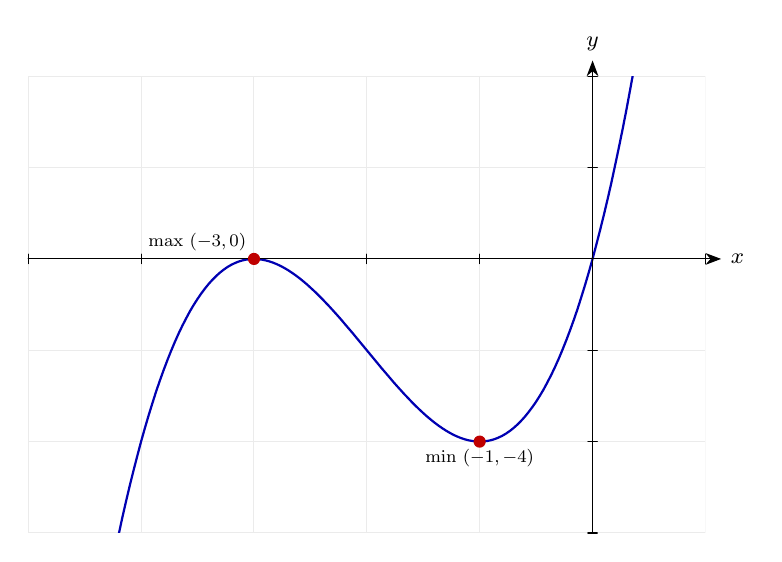
\begin{tikzpicture}[>={Stealth[length=2mm]},font=\footnotesize,line cap=round,line join=round]
\begin{scope}
\clip (0,0) rectangle (8.6,5.8);
\draw[gray!16] (0,0) grid[xstep=1.433,ystep=1.16] (8.6,5.8);
\draw[blue!70!black,thick] (0,-5.8) -- (0.048,-5.8) -- (0.096,-5.8) -- (0.143,-5.8) -- (0.191,-5.8) -- (0.239,-5.8) -- (0.287,-5.54) -- (0.334,-5.149) -- (0.382,-4.768) -- (0.43,-4.398) -- (0.478,-4.039) -- (0.526,-3.689) -- (0.573,-3.35) -- (0.621,-3.021) -- (0.669,-2.702) -- (0.717,-2.392) -- (0.764,-2.093) -- (0.812,-1.803) -- (0.86,-1.522) -- (0.908,-1.25) -- (0.956,-0.988) -- (1.003,-0.735) -- (1.051,-0.49) -- (1.099,-0.255) -- (1.147,-0.028) -- (1.194,0.191) -- (1.242,0.401) -- (1.29,0.603) -- (1.338,0.796) -- (1.386,0.982) -- (1.433,1.16) -- (1.481,1.33) -- (1.529,1.493) -- (1.577,1.648) -- (1.624,1.796) -- (1.672,1.936) -- (1.72,2.069) -- (1.768,2.196) -- (1.816,2.316) -- (1.863,2.428) -- (1.911,2.535) -- (1.959,2.635) -- (2.007,2.728) -- (2.054,2.816) -- (2.102,2.897) -- (2.15,2.972) -- (2.198,3.042) -- (2.246,3.106) -- (2.293,3.164) -- (2.341,3.217) -- (2.389,3.265) -- (2.437,3.308) -- (2.484,3.345) -- (2.532,3.378) -- (2.58,3.406) -- (2.628,3.429) -- (2.676,3.448) -- (2.723,3.462) -- (2.771,3.472) -- (2.819,3.478) -- (2.867,3.48) -- (2.914,3.478) -- (2.962,3.472) -- (3.01,3.463) -- (3.058,3.45) -- (3.106,3.434) -- (3.153,3.415) -- (3.201,3.393) -- (3.249,3.367) -- (3.297,3.339) -- (3.344,3.308) -- (3.392,3.275) -- (3.44,3.239) -- (3.488,3.2) -- (3.536,3.16) -- (3.583,3.117) -- (3.631,3.073) -- (3.679,3.027) -- (3.727,2.979) -- (3.774,2.929) -- (3.822,2.879) -- (3.87,2.826) -- (3.918,2.773) -- (3.966,2.719) -- (4.013,2.663) -- (4.061,2.607) -- (4.109,2.551) -- (4.157,2.493) -- (4.204,2.436) -- (4.252,2.378) -- (4.3,2.32) -- (4.348,2.262) -- (4.396,2.204) -- (4.443,2.147) -- (4.491,2.089) -- (4.539,2.033) -- (4.587,1.977) -- (4.634,1.921) -- (4.682,1.867) -- (4.73,1.814) -- (4.778,1.761) -- (4.826,1.711) -- (4.873,1.661) -- (4.921,1.613) -- (4.969,1.567) -- (5.017,1.522) -- (5.064,1.48) -- (5.112,1.44) -- (5.16,1.401) -- (5.208,1.365) -- (5.256,1.332) -- (5.303,1.301) -- (5.351,1.273) -- (5.399,1.247) -- (5.447,1.225) -- (5.494,1.206) -- (5.542,1.19) -- (5.59,1.177) -- (5.638,1.168) -- (5.686,1.162) -- (5.733,1.16) -- (5.781,1.162) -- (5.829,1.168) -- (5.877,1.178) -- (5.924,1.192) -- (5.972,1.211) -- (6.02,1.234) -- (6.068,1.262) -- (6.116,1.295) -- (6.163,1.332) -- (6.211,1.375) -- (6.259,1.423) -- (6.307,1.476) -- (6.354,1.534) -- (6.402,1.598) -- (6.45,1.667) -- (6.498,1.743) -- (6.546,1.824) -- (6.593,1.912) -- (6.641,2.005) -- (6.689,2.105) -- (6.737,2.212) -- (6.784,2.324) -- (6.832,2.444) -- (6.88,2.571) -- (6.928,2.704) -- (6.976,2.844) -- (7.023,2.992) -- (7.071,3.147) -- (7.119,3.31) -- (7.167,3.48) -- (7.214,3.658) -- (7.262,3.844) -- (7.31,4.037) -- (7.358,4.239) -- (7.406,4.449) -- (7.453,4.668) -- (7.501,4.895) -- (7.549,5.13) -- (7.597,5.375) -- (7.644,5.628) -- (7.692,5.89) -- (7.74,6.162) -- (7.788,6.443) -- (7.836,6.733) -- (7.883,7.032) -- (7.931,7.342) -- (7.979,7.661) -- (8.027,7.99) -- (8.074,8.329) -- (8.122,8.679) -- (8.17,9.038) -- (8.218,9.408) -- (8.266,9.789) -- (8.313,10.18) -- (8.361,10.582) -- (8.409,10.995) -- (8.457,11.42) -- (8.504,11.6) -- (8.552,11.6) -- (8.6,11.6);
\end{scope}
\draw[->] (0,3.48) -- (8.8,3.48) node[right]{$x$};
\draw[->] (7.167,0) -- (7.167,6) node[above]{$y$};
\draw (0,3.42) -- (0,3.54);
\draw (1.433,3.42) -- (1.433,3.54);
\draw (2.867,3.42) -- (2.867,3.54);
\draw (4.3,3.42) -- (4.3,3.54);
\draw (5.733,3.42) -- (5.733,3.54);
\draw (8.6,3.42) -- (8.6,3.54);
\draw (7.107,0) -- (7.227,0);
\draw (7.107,1.16) -- (7.227,1.16);
\draw (7.107,2.32) -- (7.227,2.32);
\draw (7.107,4.64) -- (7.227,4.64);
\draw (7.107,5.8) -- (7.227,5.8);
\fill[red!75!black] (2.867,3.48) circle (2.2pt);
\node[above left,scale=0.8] at (2.867,3.48) {max $(-3,0)$};
\fill[red!75!black] (5.733,1.16) circle (2.2pt);
\node[below,scale=0.8] at (5.733,1.16) {min $(-1,-4)$};
\end{tikzpicture}
}
\end{center}
\small Curve with classified stationary points marked.\normalsize

\medskip\hrule

\section*{Derivatives and Graphs 33\quad\small\texttt{(d4-033)}}
\addcontentsline{toc}{section}{Derivatives and Graphs 33 (d4-033)}
\textit{Difficulty: Foundation \quad\textbar\quad Marks: 9}

\question{The curve \( C \) has equation \( y = x^4 - 4x^3 + 4 \). (a) Find \( \dfrac{\mathrm{d}y}{\mathrm{d}x} \) and \( \dfrac{\mathrm{d}^2y}{\mathrm{d}x^2} \). (b) Find the coordinates of all stationary points and determine their nature. (c) Find the range of values of \( x \) for which \( C \) is decreasing.}

\textbf{Worked solution.}

\textit{Step 1: (a) First derivative.}
\[\begin{gathered}
\frac{\mathrm{d}y}{\mathrm{d}x} = 4x^3 - 12x^2
\end{gathered}\]
Power rule.

\textit{Step 2: Second derivative.}
\[\begin{gathered}
\frac{\mathrm{d}^2y}{\mathrm{d}x^2} = 12x^2 - 24x
\end{gathered}\]
Differentiate the first derivative.

\textit{Step 3: (b) Solve \( 4x^3 - 12x^2 = 0 \).}
\[\begin{gathered}
4x^2(x-3) = 0 \implies x=0 \text{ or } x=3
\end{gathered}\]
Factorise.

\textit{Step 4: Coordinates.}
\[\begin{gathered}
y(0) = 4; \quad y(3) = 81 - 108 + 4 = -23
\end{gathered}\]
Substitute into the original.

\textit{Step 5: Classify.}
\[\begin{gathered}
x=0: 0-0=0 \Rightarrow \text{inconclusive - check signs either side} \newline x=3: 12(9)-24(3)=108-72=36>0 \Rightarrow \text{minimum}
\end{gathered}\]
At \( x = 0 \): for \( x < 0 \), \( 4x^2 > 0 \) and \( (x-3) < 0 \), so \( \frac{\mathrm{d}y}{\mathrm{d}x} < 0 \). For small \( x > 0 \), \( 4x^2 > 0 \) and \( (x-3) < 0 \), so \( \frac{\mathrm{d}y}{\mathrm{d}x} < 0 \). Gradient does not change sign $\to$ point of inflection at \( (0, 4) \).

\textit{Step 6: (c) Decreasing: \( 4x^2(x-3) < 0 \).}
\[\begin{gathered}
4x^2 \geq 0 \text{ always; so need } (x-3) < 0 \text{ and } x \neq 0
\end{gathered}\]
Since \( 4x^2 \geq 0 \), the sign of the product depends on \( (x-3) \). The curve is decreasing when \( x < 3 \) (and \( x \neq 0 \), where the gradient is momentarily zero).

\begin{answerbox}
\textbf{Final answer:}\quad (a) \(\displaystyle  \dfrac{\mathrm{d}y}{\mathrm{d}x} = 4x^3-12x^2 \), \(\displaystyle  \dfrac{\mathrm{d}^2y}{\mathrm{d}x^2} = 12x^2-24x \) \\[3pt]  (b) Point of inflection at \(\displaystyle  (0,4) \); local minimum at \(\displaystyle  (3,-23) \) \\[3pt]  (c) Decreasing for \(\displaystyle  x < 3 \), \(\displaystyle  x \neq 0 \)
\end{answerbox}
\textbf{Diagram.}

\begin{center}
\resizebox{\ifdim\width>\linewidth \linewidth\else \width\fi}{!}{%
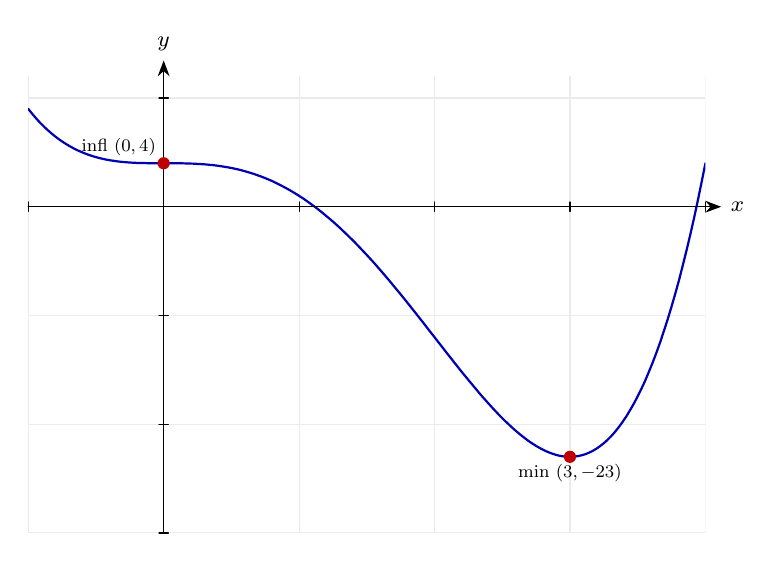
\begin{tikzpicture}[>={Stealth[length=2mm]},font=\footnotesize,line cap=round,line join=round]
\begin{scope}
\clip (0,0) rectangle (8.6,5.8);
\draw[gray!16] (0,0) grid[xstep=1.72,ystep=1.381] (8.6,5.8);
\draw[blue!70!black,thick] (0,5.386) -- (0.048,5.326) -- (0.096,5.27) -- (0.143,5.218) -- (0.191,5.169) -- (0.239,5.124) -- (0.287,5.081) -- (0.334,5.042) -- (0.382,5.006) -- (0.43,4.972) -- (0.478,4.941) -- (0.526,4.912) -- (0.573,4.886) -- (0.621,4.862) -- (0.669,4.841) -- (0.717,4.821) -- (0.764,4.803) -- (0.812,4.787) -- (0.86,4.773) -- (0.908,4.76) -- (0.956,4.749) -- (1.003,4.739) -- (1.051,4.731) -- (1.099,4.724) -- (1.147,4.717) -- (1.194,4.712) -- (1.242,4.708) -- (1.29,4.704) -- (1.338,4.702) -- (1.386,4.699) -- (1.433,4.698) -- (1.481,4.697) -- (1.529,4.696) -- (1.577,4.696) -- (1.624,4.695) -- (1.672,4.695) -- (1.72,4.695) -- (1.768,4.695) -- (1.816,4.695) -- (1.863,4.695) -- (1.911,4.695) -- (1.959,4.694) -- (2.007,4.693) -- (2.054,4.691) -- (2.102,4.69) -- (2.15,4.687) -- (2.198,4.684) -- (2.246,4.681) -- (2.293,4.676) -- (2.341,4.672) -- (2.389,4.666) -- (2.437,4.659) -- (2.484,4.652) -- (2.532,4.644) -- (2.58,4.635) -- (2.628,4.625) -- (2.676,4.614) -- (2.723,4.602) -- (2.771,4.588) -- (2.819,4.574) -- (2.867,4.559) -- (2.914,4.542) -- (2.962,4.525) -- (3.01,4.506) -- (3.058,4.486) -- (3.106,4.465) -- (3.153,4.442) -- (3.201,4.418) -- (3.249,4.393) -- (3.297,4.367) -- (3.344,4.34) -- (3.392,4.311) -- (3.44,4.281) -- (3.488,4.25) -- (3.536,4.217) -- (3.583,4.183) -- (3.631,4.148) -- (3.679,4.112) -- (3.727,4.074) -- (3.774,4.035) -- (3.822,3.995) -- (3.87,3.954) -- (3.918,3.911) -- (3.966,3.867) -- (4.013,3.822) -- (4.061,3.776) -- (4.109,3.729) -- (4.157,3.681) -- (4.204,3.632) -- (4.252,3.581) -- (4.3,3.53) -- (4.348,3.478) -- (4.396,3.425) -- (4.443,3.371) -- (4.491,3.316) -- (4.539,3.26) -- (4.587,3.203) -- (4.634,3.146) -- (4.682,3.088) -- (4.73,3.03) -- (4.778,2.971) -- (4.826,2.911) -- (4.873,2.852) -- (4.921,2.791) -- (4.969,2.73) -- (5.017,2.67) -- (5.064,2.608) -- (5.112,2.547) -- (5.16,2.486) -- (5.208,2.424) -- (5.256,2.363) -- (5.303,2.302) -- (5.351,2.241) -- (5.399,2.18) -- (5.447,2.12) -- (5.494,2.06) -- (5.542,2.001) -- (5.59,1.943) -- (5.638,1.885) -- (5.686,1.828) -- (5.733,1.771) -- (5.781,1.716) -- (5.829,1.662) -- (5.877,1.609) -- (5.924,1.558) -- (5.972,1.507) -- (6.02,1.459) -- (6.068,1.411) -- (6.116,1.366) -- (6.163,1.322) -- (6.211,1.281) -- (6.259,1.241) -- (6.307,1.204) -- (6.354,1.168) -- (6.402,1.136) -- (6.45,1.105) -- (6.498,1.078) -- (6.546,1.053) -- (6.593,1.031) -- (6.641,1.012) -- (6.689,0.996) -- (6.737,0.983) -- (6.784,0.974) -- (6.832,0.969) -- (6.88,0.967) -- (6.928,0.969) -- (6.976,0.975) -- (7.023,0.985) -- (7.071,0.999) -- (7.119,1.018) -- (7.167,1.041) -- (7.214,1.069) -- (7.262,1.102) -- (7.31,1.14) -- (7.358,1.183) -- (7.406,1.231) -- (7.453,1.285) -- (7.501,1.345) -- (7.549,1.411) -- (7.597,1.482) -- (7.644,1.56) -- (7.692,1.644) -- (7.74,1.735) -- (7.788,1.832) -- (7.836,1.936) -- (7.883,2.048) -- (7.931,2.166) -- (7.979,2.292) -- (8.027,2.426) -- (8.074,2.568) -- (8.122,2.717) -- (8.17,2.875) -- (8.218,3.041) -- (8.266,3.215) -- (8.313,3.399) -- (8.361,3.591) -- (8.409,3.793) -- (8.457,4.004) -- (8.504,4.224) -- (8.552,4.455) -- (8.6,4.695);
\end{scope}
\draw[->] (0,4.143) -- (8.8,4.143) node[right]{$x$};
\draw[->] (1.72,0) -- (1.72,6) node[above]{$y$};
\draw (0,4.083) -- (0,4.203);
\draw (3.44,4.083) -- (3.44,4.203);
\draw (5.16,4.083) -- (5.16,4.203);
\draw (6.88,4.083) -- (6.88,4.203);
\draw (8.6,4.083) -- (8.6,4.203);
\draw (1.66,0) -- (1.78,0);
\draw (1.66,1.381) -- (1.78,1.381);
\draw (1.66,2.762) -- (1.78,2.762);
\draw (1.66,5.524) -- (1.78,5.524);
\fill[red!75!black] (1.72,4.695) circle (2.2pt);
\node[above left,scale=0.8] at (1.72,4.695) {infl $(0,4)$};
\fill[red!75!black] (6.88,0.967) circle (2.2pt);
\node[below,scale=0.8] at (6.88,0.967) {min $(3,-23)$};
\end{tikzpicture}
}
\end{center}
\small Curve with classified stationary points marked.\normalsize

\medskip\hrule

\section*{Derivatives and Graphs 34\quad\small\texttt{(d4-034)}}
\addcontentsline{toc}{section}{Derivatives and Graphs 34 (d4-034)}
\textit{Difficulty: Foundation \quad\textbar\quad Marks: 8}

\question{The curve \( y = x^3 + ax^2 + bx + c \) has a stationary point at \( (3, 27) \) and \( \dfrac{\mathrm{d}^2y}{\mathrm{d}x^2} = 0 \) at \( (3, 27) \). Given also that the curve passes through the origin, find \( a \), \( b \), and \( c \).}

\textbf{Worked solution.}

\textit{Step 1: The curve passes through the origin: \( c = 0 \).}
\[\begin{gathered}
x=0, y=0: 0+0+0+c=0 \implies c=0
\end{gathered}\]
Substitute the known point \( (0,0) \).

\textit{Step 2: The curve passes through \( (3, 27) \).}
\[\begin{gathered}
27 + 9a + 3b = 27 \implies 9a + 3b = 0 \implies 3a + b = 0 \quad \cdots (1)
\end{gathered}\]
Substitute \( x=3, y=27 \) with \( c = 0 \) to obtain one equation in \( a \) and \( b \).

\textit{Step 3: Stationary point at \( x = 3 \): \( \dfrac{\mathrm{d}y}{\mathrm{d}x} = 0 \).}
\[\begin{gathered}
\frac{\mathrm{d}y}{\mathrm{d}x} = 3x^2 + 2ax + b \newline 27 + 6a + b = 0 \quad \cdots (2)
\end{gathered}\]
Differentiate, substitute \( x = 3 \) and set the gradient to zero, since a stationary point has zero gradient.

\textit{Step 4: \( \dfrac{\mathrm{d}^2y}{\mathrm{d}x^2} = 0 \) at \( x = 3 \).}
\[\begin{gathered}
\frac{\mathrm{d}^2y}{\mathrm{d}x^2} = 6x + 2a \newline 18 + 2a = 0 \implies a = -9 \quad \cdots (3)
\end{gathered}\]
Differentiating once more and setting \( \dfrac{\mathrm{d}^2y}{\mathrm{d}x^2} = 0 \) pins down \( a \) directly. A simultaneous \( y'=0 \) and \( y''=0 \) at the same point signals a stationary point of inflection.

\textit{Step 5: Find \( b \) from equation (2).}
\[\begin{gathered}
27 + 6(-9) + b = 0 \implies 27 - 54 + b = 0 \implies b = 27
\end{gathered}\]
Back-substitute \( a = -9 \) into (2) to solve for \( b \).

\textit{Step 6: Verify with equation (1).}
\[\begin{gathered}
3(-9) + 27 = -27 + 27 = 0 \checkmark
\end{gathered}\]
Equation (1) is satisfied, so the three conditions are consistent. The cubic \( y = x^3 - 9x^2 + 27x = (x-3)^3 + 27 \) has a stationary point of inflection at \( (3, 27) \) and passes through the origin, as required.

\begin{answerbox}
\textbf{Final answer:}\quad \(\displaystyle  a = -9,\; b = 27,\; c = 0 \)
\end{answerbox}
\textbf{Diagram.}

\begin{center}
\resizebox{\ifdim\width>\linewidth \linewidth\else \width\fi}{!}{%
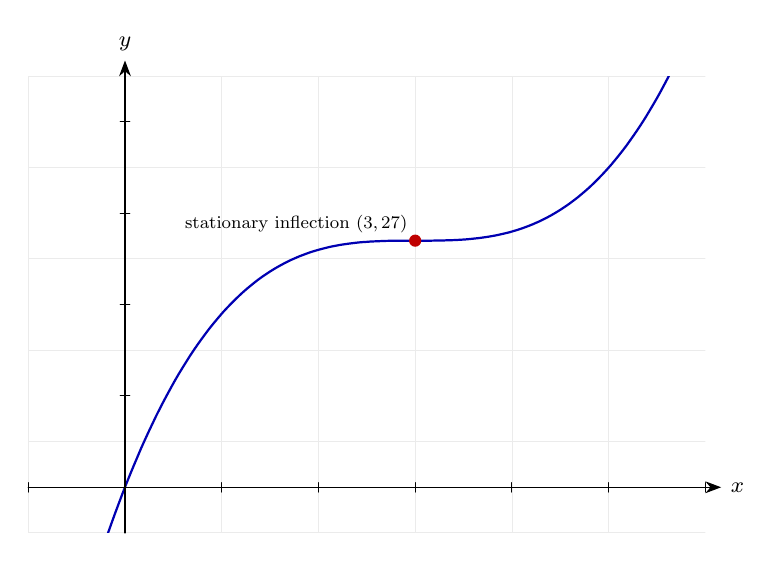
\begin{tikzpicture}[>={Stealth[length=2mm]},font=\footnotesize,line cap=round,line join=round]
\begin{scope}
\clip (0,0) rectangle (8.6,5.8);
\draw[gray!16] (0,-0.58) grid[xstep=1.229,ystep=1.16] (8.6,5.8);
\draw[blue!70!black,thick] (0,-3.712) -- (0.048,-3.498) -- (0.096,-3.287) -- (0.143,-3.081) -- (0.191,-2.879) -- (0.239,-2.681) -- (0.287,-2.487) -- (0.334,-2.297) -- (0.382,-2.111) -- (0.43,-1.929) -- (0.478,-1.75) -- (0.526,-1.576) -- (0.573,-1.405) -- (0.621,-1.238) -- (0.669,-1.074) -- (0.717,-0.915) -- (0.764,-0.758) -- (0.812,-0.606) -- (0.86,-0.457) -- (0.908,-0.311) -- (0.956,-0.169) -- (1.003,-0.03) -- (1.051,0.105) -- (1.099,0.238) -- (1.147,0.367) -- (1.194,0.492) -- (1.242,0.615) -- (1.29,0.734) -- (1.338,0.85) -- (1.386,0.963) -- (1.433,1.074) -- (1.481,1.181) -- (1.529,1.285) -- (1.577,1.386) -- (1.624,1.485) -- (1.672,1.58) -- (1.72,1.673) -- (1.768,1.763) -- (1.816,1.851) -- (1.863,1.936) -- (1.911,2.018) -- (1.959,2.097) -- (2.007,2.174) -- (2.054,2.249) -- (2.102,2.321) -- (2.15,2.391) -- (2.198,2.458) -- (2.246,2.523) -- (2.293,2.586) -- (2.341,2.646) -- (2.389,2.704) -- (2.437,2.761) -- (2.484,2.815) -- (2.532,2.866) -- (2.58,2.916) -- (2.628,2.964) -- (2.676,3.01) -- (2.723,3.054) -- (2.771,3.096) -- (2.819,3.136) -- (2.867,3.175) -- (2.914,3.212) -- (2.962,3.247) -- (3.01,3.28) -- (3.058,3.312) -- (3.106,3.342) -- (3.153,3.37) -- (3.201,3.397) -- (3.249,3.423) -- (3.297,3.447) -- (3.344,3.47) -- (3.392,3.491) -- (3.44,3.512) -- (3.488,3.53) -- (3.536,3.548) -- (3.583,3.565) -- (3.631,3.58) -- (3.679,3.594) -- (3.727,3.607) -- (3.774,3.619) -- (3.822,3.631) -- (3.87,3.641) -- (3.918,3.65) -- (3.966,3.659) -- (4.013,3.666) -- (4.061,3.673) -- (4.109,3.679) -- (4.157,3.685) -- (4.204,3.69) -- (4.252,3.694) -- (4.3,3.697) -- (4.348,3.701) -- (4.396,3.703) -- (4.443,3.705) -- (4.491,3.707) -- (4.539,3.709) -- (4.587,3.71) -- (4.634,3.711) -- (4.682,3.711) -- (4.73,3.712) -- (4.778,3.712) -- (4.826,3.712) -- (4.873,3.712) -- (4.921,3.712) -- (4.969,3.712) -- (5.017,3.712) -- (5.064,3.712) -- (5.112,3.712) -- (5.16,3.713) -- (5.208,3.714) -- (5.256,3.714) -- (5.303,3.716) -- (5.351,3.717) -- (5.399,3.719) -- (5.447,3.721) -- (5.494,3.724) -- (5.542,3.727) -- (5.59,3.731) -- (5.638,3.736) -- (5.686,3.741) -- (5.733,3.746) -- (5.781,3.753) -- (5.829,3.76) -- (5.877,3.768) -- (5.924,3.776) -- (5.972,3.786) -- (6.02,3.797) -- (6.068,3.808) -- (6.116,3.82) -- (6.163,3.834) -- (6.211,3.848) -- (6.259,3.864) -- (6.307,3.881) -- (6.354,3.899) -- (6.402,3.918) -- (6.45,3.939) -- (6.498,3.96) -- (6.546,3.984) -- (6.593,4.008) -- (6.641,4.034) -- (6.689,4.062) -- (6.737,4.091) -- (6.784,4.121) -- (6.832,4.153) -- (6.88,4.187) -- (6.928,4.223) -- (6.976,4.26) -- (7.023,4.299) -- (7.071,4.34) -- (7.119,4.382) -- (7.167,4.427) -- (7.214,4.473) -- (7.262,4.522) -- (7.31,4.572) -- (7.358,4.625) -- (7.406,4.679) -- (7.453,4.736) -- (7.501,4.795) -- (7.549,4.856) -- (7.597,4.919) -- (7.644,4.985) -- (7.692,5.053) -- (7.74,5.123) -- (7.788,5.196) -- (7.836,5.271) -- (7.883,5.349) -- (7.931,5.43) -- (7.979,5.512) -- (8.027,5.598) -- (8.074,5.686) -- (8.122,5.777) -- (8.17,5.871) -- (8.218,5.967) -- (8.266,6.066) -- (8.313,6.169) -- (8.361,6.274) -- (8.409,6.382) -- (8.457,6.493) -- (8.504,6.607) -- (8.552,6.724) -- (8.6,6.844);
\end{scope}
\draw[->] (0,0.58) -- (8.8,0.58) node[right]{$x$};
\draw[->] (1.229,0) -- (1.229,6) node[above]{$y$};
\draw (0,0.52) -- (0,0.64);
\draw (2.457,0.52) -- (2.457,0.64);
\draw (3.686,0.52) -- (3.686,0.64);
\draw (4.914,0.52) -- (4.914,0.64);
\draw (6.143,0.52) -- (6.143,0.64);
\draw (7.371,0.52) -- (7.371,0.64);
\draw (8.6,0.52) -- (8.6,0.64);
\draw (1.169,1.74) -- (1.289,1.74);
\draw (1.169,2.9) -- (1.289,2.9);
\draw (1.169,4.06) -- (1.289,4.06);
\draw (1.169,5.22) -- (1.289,5.22);
\fill[red!75!black] (4.914,3.712) circle (2.2pt);
\node[above left,scale=0.8] at (4.914,3.712) {stationary inflection $(3,27)$};
\end{tikzpicture}
}
\end{center}
\small Curve with classified stationary points marked.\normalsize

\medskip\hrule

\section*{Derivatives and Graphs 35\quad\small\texttt{(d4-035)}}
\addcontentsline{toc}{section}{Derivatives and Graphs 35 (d4-035)}
\textit{Difficulty: Foundation \quad\textbar\quad Marks: 10}

\question{A manufacturer models the cost \( C \) (\pounds  thousands) of producing \( x \) hundred units as \( C(x) = x^3 - 9x^2 + 24x + 10 \) for \( 0 \leq x \leq 6 \). (a) Find \( C'(x) \). (b) Find the stationary points of \( C \) and classify them. (c) State the values of \( x \) for which \( C \) is decreasing, and explain what this means in context. (d) Find the minimum cost in the given domain.}

\textbf{Worked solution.}

\textit{Step 1: (a) Differentiate.}
\[\begin{gathered}
C'(x) = 3x^2 - 18x + 24
\end{gathered}\]
Power rule.

\textit{Step 2: (b) Solve \( C'(x) = 0 \).}
\[\begin{gathered}
3x^2 - 18x + 24 = 0 \implies x^2 - 6x + 8 = 0 \implies (x-2)(x-4) = 0
\end{gathered}\]
Divide by 3 and factorise.

\textit{Step 3: Coordinates.}
\[\begin{gathered}
C(2) = 8 - 36 + 48 + 10 = 30; \quad C(4) = 64 - 144 + 96 + 10 = 26
\end{gathered}\]
Substitute \( x = 2 \) and \( x = 4 \) into \( C(x) \).

\textit{Step 4: Second derivative.}
\[\begin{gathered}
C''(x) = 6x - 18 \newline C''(2) = -6 < 0 \Rightarrow \text{local maximum} \newline C''(4) = 6 > 0 \Rightarrow \text{local minimum}
\end{gathered}\]
Apply the second derivative test.

\textit{Step 5: (c) Decreasing: \( C'(x) < 0 \).}
\[\begin{gathered}
(x-2)(x-4) < 0 \implies 2 < x < 4
\end{gathered}\]
In context: costs are falling (economies of scale) between producing 200 and 400 units.

\textit{Step 6: (d) Compare the local minimum \( C(4) = 26 \) with the endpoint \( C(0) = 10 \) and \( C(6) = 216 - 324 + 144 + 10 = 46 \).}
\[\begin{gathered}
\min\{C(0), C(4), C(6)\} = \min\{10, 26, 46\} = 10
\end{gathered}\]
Always check endpoints when optimising over a closed interval.

\begin{answerbox}
\textbf{Final answer:}\quad (a) \(\displaystyle  C'(x) = 3x^2-18x+24 \) \\[3pt]  (b) Local max at \(\displaystyle  (2, 30) \); local min at \(\displaystyle  (4, 26) \) \\[3pt]  (c) Decreasing for \(\displaystyle  2 < x < 4 \) --- costs fall as production rises from 200 to 400 units \\[3pt]  (d) Minimum cost is \pounds 10\,000 (at \(\displaystyle  x = 0 \))
\end{answerbox}
\textbf{Diagram.}

\begin{center}
\resizebox{\ifdim\width>\linewidth \linewidth\else \width\fi}{!}{%
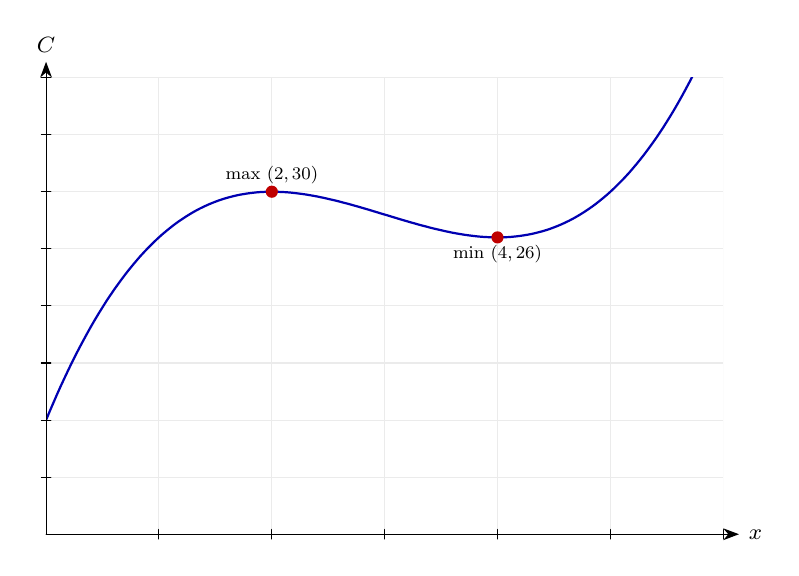
\begin{tikzpicture}[>={Stealth[length=2mm]},font=\footnotesize,line cap=round,line join=round]
\begin{scope}
\clip (0,0) rectangle (8.6,5.8);
\draw[gray!16] (0,0) grid[xstep=1.433,ystep=0.725] (8.6,5.8);
\draw[blue!70!black,thick] (0,1.45) -- (0.048,1.565) -- (0.096,1.676) -- (0.143,1.785) -- (0.191,1.891) -- (0.239,1.994) -- (0.287,2.095) -- (0.334,2.193) -- (0.382,2.288) -- (0.43,2.38) -- (0.478,2.47) -- (0.526,2.558) -- (0.573,2.642) -- (0.621,2.725) -- (0.669,2.805) -- (0.717,2.882) -- (0.764,2.957) -- (0.812,3.029) -- (0.86,3.1) -- (0.908,3.167) -- (0.956,3.233) -- (1.003,3.296) -- (1.051,3.357) -- (1.099,3.416) -- (1.147,3.473) -- (1.194,3.528) -- (1.242,3.58) -- (1.29,3.631) -- (1.338,3.679) -- (1.386,3.726) -- (1.433,3.77) -- (1.481,3.813) -- (1.529,3.853) -- (1.577,3.892) -- (1.624,3.929) -- (1.672,3.964) -- (1.72,3.997) -- (1.768,4.029) -- (1.816,4.059) -- (1.863,4.087) -- (1.911,4.114) -- (1.959,4.139) -- (2.007,4.162) -- (2.054,4.184) -- (2.102,4.204) -- (2.15,4.223) -- (2.198,4.241) -- (2.246,4.257) -- (2.293,4.271) -- (2.341,4.284) -- (2.389,4.296) -- (2.437,4.307) -- (2.484,4.316) -- (2.532,4.324) -- (2.58,4.331) -- (2.628,4.337) -- (2.676,4.342) -- (2.723,4.346) -- (2.771,4.348) -- (2.819,4.35) -- (2.867,4.35) -- (2.914,4.35) -- (2.962,4.348) -- (3.01,4.346) -- (3.058,4.343) -- (3.106,4.339) -- (3.153,4.334) -- (3.201,4.328) -- (3.249,4.322) -- (3.297,4.315) -- (3.344,4.307) -- (3.392,4.299) -- (3.44,4.29) -- (3.488,4.28) -- (3.536,4.27) -- (3.583,4.259) -- (3.631,4.248) -- (3.679,4.237) -- (3.727,4.225) -- (3.774,4.212) -- (3.822,4.2) -- (3.87,4.187) -- (3.918,4.173) -- (3.966,4.16) -- (4.013,4.146) -- (4.061,4.132) -- (4.109,4.118) -- (4.157,4.103) -- (4.204,4.089) -- (4.252,4.074) -- (4.3,4.06) -- (4.348,4.046) -- (4.396,4.031) -- (4.443,4.017) -- (4.491,4.002) -- (4.539,3.988) -- (4.587,3.974) -- (4.634,3.96) -- (4.682,3.947) -- (4.73,3.933) -- (4.778,3.92) -- (4.826,3.908) -- (4.873,3.895) -- (4.921,3.883) -- (4.969,3.872) -- (5.017,3.861) -- (5.064,3.85) -- (5.112,3.84) -- (5.16,3.83) -- (5.208,3.821) -- (5.256,3.813) -- (5.303,3.805) -- (5.351,3.798) -- (5.399,3.792) -- (5.447,3.786) -- (5.494,3.781) -- (5.542,3.777) -- (5.59,3.774) -- (5.638,3.772) -- (5.686,3.77) -- (5.733,3.77) -- (5.781,3.77) -- (5.829,3.772) -- (5.877,3.774) -- (5.924,3.778) -- (5.972,3.783) -- (6.02,3.789) -- (6.068,3.796) -- (6.116,3.804) -- (6.163,3.813) -- (6.211,3.824) -- (6.259,3.836) -- (6.307,3.849) -- (6.354,3.863) -- (6.402,3.879) -- (6.45,3.897) -- (6.498,3.916) -- (6.546,3.936) -- (6.593,3.958) -- (6.641,3.981) -- (6.689,4.006) -- (6.737,4.033) -- (6.784,4.061) -- (6.832,4.091) -- (6.88,4.123) -- (6.928,4.156) -- (6.976,4.191) -- (7.023,4.228) -- (7.071,4.267) -- (7.119,4.307) -- (7.167,4.35) -- (7.214,4.394) -- (7.262,4.441) -- (7.31,4.489) -- (7.358,4.54) -- (7.406,4.592) -- (7.453,4.647) -- (7.501,4.704) -- (7.549,4.763) -- (7.597,4.824) -- (7.644,4.887) -- (7.692,4.953) -- (7.74,5.02) -- (7.788,5.091) -- (7.836,5.163) -- (7.883,5.238) -- (7.931,5.315) -- (7.979,5.395) -- (8.027,5.478) -- (8.074,5.562) -- (8.122,5.65) -- (8.17,5.74) -- (8.218,5.832) -- (8.266,5.927) -- (8.313,6.025) -- (8.361,6.126) -- (8.409,6.229) -- (8.457,6.335) -- (8.504,6.444) -- (8.552,6.555) -- (8.6,6.67);
\end{scope}
\draw[->] (0,0) -- (8.8,0) node[right]{$x$};
\draw[->] (0,0) -- (0,6) node[above]{$C$};
\draw (1.433,-0.06) -- (1.433,0.06);
\draw (2.867,-0.06) -- (2.867,0.06);
\draw (4.3,-0.06) -- (4.3,0.06);
\draw (5.733,-0.06) -- (5.733,0.06);
\draw (7.167,-0.06) -- (7.167,0.06);
\draw (8.6,-0.06) -- (8.6,0.06);
\draw (-0.06,0.725) -- (0.06,0.725);
\draw (-0.06,1.45) -- (0.06,1.45);
\draw (-0.06,2.175) -- (0.06,2.175);
\draw (-0.06,2.9) -- (0.06,2.9);
\draw (-0.06,3.625) -- (0.06,3.625);
\draw (-0.06,4.35) -- (0.06,4.35);
\draw (-0.06,5.075) -- (0.06,5.075);
\draw (-0.06,5.8) -- (0.06,5.8);
\fill[red!75!black] (2.867,4.35) circle (2.2pt);
\node[above,scale=0.8] at (2.867,4.35) {max $(2,30)$};
\fill[red!75!black] (5.733,3.77) circle (2.2pt);
\node[below,scale=0.8] at (5.733,3.77) {min $(4,26)$};
\end{tikzpicture}
}
\end{center}
\small Curve with classified stationary points marked.\normalsize

\medskip\hrule

\section*{Derivatives and Graphs 36\quad\small\texttt{(d4-036)}}
\addcontentsline{toc}{section}{Derivatives and Graphs 36 (d4-036)}
\textit{Difficulty: Standard \quad\textbar\quad Marks: 6}

\question{Find the stationary points of \( y = x^3 - 3x^2 - 9x + 1 \) and use the first derivative sign test to classify them.}

\textbf{Worked solution.}

\textit{Step 1: Differentiate and factorise.}
\[\begin{gathered}
\frac{\mathrm{d}y}{\mathrm{d}x} = 3x^2 - 6x - 9 = 3(x-3)(x+1)
\end{gathered}\]
Factor out 3, then factorise the quadratic.

\textit{Step 2: Set to zero.}
\[\begin{gathered}
x = -1 \text{ or } x = 3
\end{gathered}\]
Two stationary points.

\textit{Step 3: Find \( y \).}
\[\begin{gathered}
y(-1) = -1 - 3 + 9 + 1 = 6 \\ y(3) = 27 - 27 - 27 + 1 = -26
\end{gathered}\]
Substitute back.

\textit{Step 4: First derivative sign test around each point.}
\[\begin{gathered}
y'(-2) = 15 > 0, \; y'(0) = -9 < 0 \; \Rightarrow \; \text{max at } x = -1 \\ y'(0) = -9 < 0, \; y'(4) = 15 > 0 \; \Rightarrow \; \text{min at } x = 3
\end{gathered}\]
Sign goes + $\to$ $-$ $\to$ + as \( x \) increases through the two stationary points.

\begin{answerbox}
\textbf{Final answer:}\quad Maximum at \(\displaystyle  (-1, 6) \); minimum at \(\displaystyle  (3, -26) \).
\end{answerbox}
\textbf{Diagram.}

\begin{center}
\resizebox{\ifdim\width>\linewidth \linewidth\else \width\fi}{!}{%
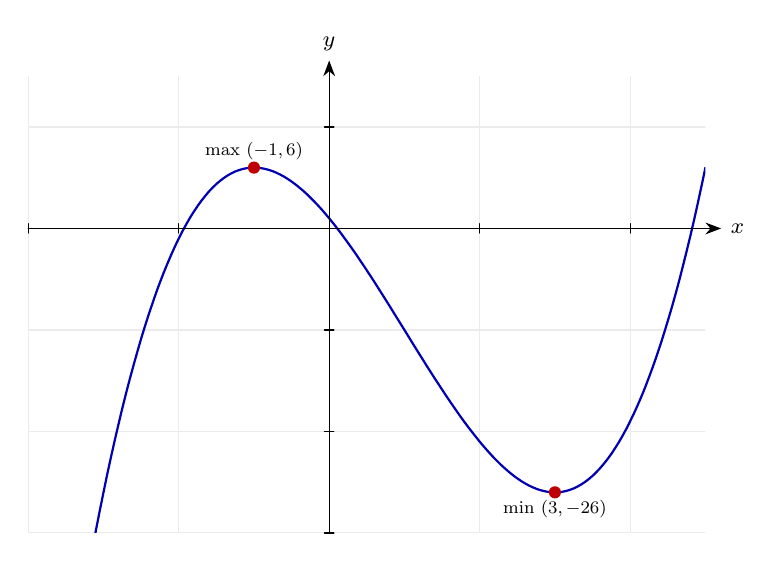
\begin{tikzpicture}[>={Stealth[length=2mm]},font=\footnotesize,line cap=round,line join=round]
\begin{scope}
\clip (0,0) rectangle (8.6,5.8);
\draw[gray!16] (0,0) grid[xstep=1.911,ystep=1.289] (8.6,5.8);
\draw[blue!70!black,thick] (0,-5.8) -- (0.048,-5.399) -- (0.096,-5.007) -- (0.143,-4.625) -- (0.191,-4.252) -- (0.239,-3.889) -- (0.287,-3.535) -- (0.334,-3.189) -- (0.382,-2.853) -- (0.43,-2.526) -- (0.478,-2.207) -- (0.526,-1.897) -- (0.573,-1.596) -- (0.621,-1.303) -- (0.669,-1.019) -- (0.717,-0.743) -- (0.764,-0.475) -- (0.812,-0.216) -- (0.86,0.036) -- (0.908,0.28) -- (0.956,0.516) -- (1.003,0.744) -- (1.051,0.964) -- (1.099,1.177) -- (1.147,1.383) -- (1.194,1.581) -- (1.242,1.772) -- (1.29,1.956) -- (1.338,2.132) -- (1.386,2.302) -- (1.433,2.465) -- (1.481,2.621) -- (1.529,2.771) -- (1.577,2.913) -- (1.624,3.05) -- (1.672,3.18) -- (1.72,3.304) -- (1.768,3.421) -- (1.816,3.533) -- (1.863,3.638) -- (1.911,3.738) -- (1.959,3.832) -- (2.007,3.92) -- (2.054,4.002) -- (2.102,4.079) -- (2.15,4.151) -- (2.198,4.217) -- (2.246,4.278) -- (2.293,4.334) -- (2.341,4.385) -- (2.389,4.431) -- (2.437,4.472) -- (2.484,4.508) -- (2.532,4.54) -- (2.58,4.567) -- (2.628,4.59) -- (2.676,4.608) -- (2.723,4.622) -- (2.771,4.632) -- (2.819,4.638) -- (2.867,4.64) -- (2.914,4.638) -- (2.962,4.632) -- (3.01,4.623) -- (3.058,4.61) -- (3.106,4.594) -- (3.153,4.574) -- (3.201,4.551) -- (3.249,4.525) -- (3.297,4.495) -- (3.344,4.463) -- (3.392,4.428) -- (3.44,4.389) -- (3.488,4.349) -- (3.536,4.305) -- (3.583,4.259) -- (3.631,4.211) -- (3.679,4.16) -- (3.727,4.108) -- (3.774,4.053) -- (3.822,3.996) -- (3.87,3.937) -- (3.918,3.876) -- (3.966,3.813) -- (4.013,3.749) -- (4.061,3.683) -- (4.109,3.616) -- (4.157,3.548) -- (4.204,3.478) -- (4.252,3.407) -- (4.3,3.335) -- (4.348,3.262) -- (4.396,3.188) -- (4.443,3.114) -- (4.491,3.038) -- (4.539,2.962) -- (4.587,2.886) -- (4.634,2.809) -- (4.682,2.732) -- (4.73,2.655) -- (4.778,2.578) -- (4.826,2.5) -- (4.873,2.423) -- (4.921,2.346) -- (4.969,2.269) -- (5.017,2.193) -- (5.064,2.117) -- (5.112,2.042) -- (5.16,1.967) -- (5.208,1.894) -- (5.256,1.821) -- (5.303,1.749) -- (5.351,1.678) -- (5.399,1.608) -- (5.447,1.539) -- (5.494,1.472) -- (5.542,1.406) -- (5.59,1.342) -- (5.638,1.28) -- (5.686,1.219) -- (5.733,1.16) -- (5.781,1.103) -- (5.829,1.048) -- (5.877,0.995) -- (5.924,0.944) -- (5.972,0.896) -- (6.02,0.85) -- (6.068,0.807) -- (6.116,0.766) -- (6.163,0.728) -- (6.211,0.693) -- (6.259,0.66) -- (6.307,0.631) -- (6.354,0.605) -- (6.402,0.582) -- (6.45,0.562) -- (6.498,0.545) -- (6.546,0.533) -- (6.593,0.523) -- (6.641,0.517) -- (6.689,0.516) -- (6.737,0.518) -- (6.784,0.523) -- (6.832,0.533) -- (6.88,0.548) -- (6.928,0.566) -- (6.976,0.589) -- (7.023,0.616) -- (7.071,0.648) -- (7.119,0.684) -- (7.167,0.725) -- (7.214,0.771) -- (7.262,0.822) -- (7.31,0.878) -- (7.358,0.939) -- (7.406,1.005) -- (7.453,1.076) -- (7.501,1.153) -- (7.549,1.236) -- (7.597,1.324) -- (7.644,1.418) -- (7.692,1.517) -- (7.74,1.623) -- (7.788,1.734) -- (7.836,1.852) -- (7.883,1.976) -- (7.931,2.106) -- (7.979,2.242) -- (8.027,2.385) -- (8.074,2.534) -- (8.122,2.691) -- (8.17,2.853) -- (8.218,3.023) -- (8.266,3.2) -- (8.313,3.384) -- (8.361,3.575) -- (8.409,3.773) -- (8.457,3.978) -- (8.504,4.191) -- (8.552,4.412) -- (8.6,4.64);
\end{scope}
\draw[->] (0,3.867) -- (8.8,3.867) node[right]{$x$};
\draw[->] (3.822,0) -- (3.822,6) node[above]{$y$};
\draw (0,3.807) -- (0,3.927);
\draw (1.911,3.807) -- (1.911,3.927);
\draw (5.733,3.807) -- (5.733,3.927);
\draw (7.644,3.807) -- (7.644,3.927);
\draw (3.762,0) -- (3.882,0);
\draw (3.762,1.289) -- (3.882,1.289);
\draw (3.762,2.578) -- (3.882,2.578);
\draw (3.762,5.156) -- (3.882,5.156);
\fill[red!75!black] (2.867,4.64) circle (2.2pt);
\node[above,scale=0.8] at (2.867,4.64) {max $(-1,6)$};
\fill[red!75!black] (6.689,0.516) circle (2.2pt);
\node[below,scale=0.8] at (6.689,0.516) {min $(3,-26)$};
\end{tikzpicture}
}
\end{center}
\small Curve with classified stationary points marked.\normalsize

\medskip\hrule

\section*{Derivatives and Graphs 37\quad\small\texttt{(d4-037)}}
\addcontentsline{toc}{section}{Derivatives and Graphs 37 (d4-037)}
\textit{Difficulty: Standard \quad\textbar\quad Marks: 6}

\question{Find the stationary points of \( y = x^3 + 3x^2 - 24x + 5 \) and classify them using the first-derivative sign test.}

\textbf{Worked solution.}

\textit{Step 1: Differentiate.}
\[\begin{gathered}
\frac{\mathrm{d}y}{\mathrm{d}x} = 3x^2 + 6x - 24
\end{gathered}\]
Apply the power rule.

\textit{Step 2: Factorise and solve.}
\[\begin{gathered}
3(x^2 + 2x - 8) = 0 \Rightarrow (x+4)(x-2) = 0
\end{gathered}\]
Two stationary points at \( x = -4 \) and \( x = 2 \).

\textit{Step 3: Compute \( y \).}
\[\begin{gathered}
y(-4) = -64 + 48 + 96 + 5 = 85 \\ y(2) = 8 + 12 - 48 + 5 = -23
\end{gathered}\]
Substitute.

\textit{Step 4: Sign test.}
\[\begin{gathered}
y'(-5) = 21 > 0,\; y'(0) = -24 < 0 \Rightarrow \text{max at } x = -4 \\ y'(0) = -24 < 0,\; y'(3) = 21 > 0 \Rightarrow \text{min at } x = 2
\end{gathered}\]
Gradient changes + $\to$ $-$ $\to$ +.

\begin{answerbox}
\textbf{Final answer:}\quad Maximum at \(\displaystyle  (-4, 85) \); minimum at \(\displaystyle  (2, -23) \).
\end{answerbox}
\textbf{Diagram.}

\begin{center}
\resizebox{\ifdim\width>\linewidth \linewidth\else \width\fi}{!}{%
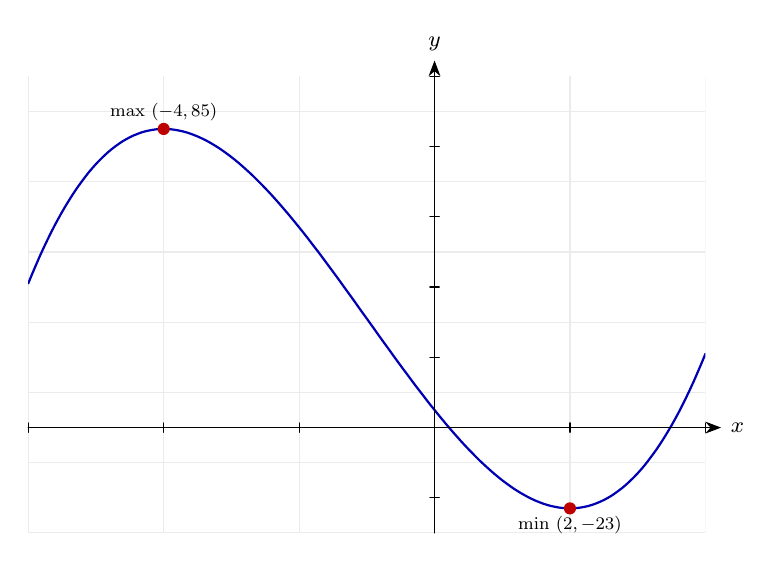
\begin{tikzpicture}[>={Stealth[length=2mm]},font=\footnotesize,line cap=round,line join=round]
\begin{scope}
\clip (0,0) rectangle (8.6,5.8);
\draw[gray!16] (0,-0.446) grid[xstep=1.72,ystep=0.892] (8.6,5.8);
\draw[blue!70!black,thick] (0,3.168) -- (0.048,3.285) -- (0.096,3.397) -- (0.143,3.506) -- (0.191,3.611) -- (0.239,3.712) -- (0.287,3.809) -- (0.334,3.902) -- (0.382,3.991) -- (0.43,4.077) -- (0.478,4.159) -- (0.526,4.237) -- (0.573,4.311) -- (0.621,4.382) -- (0.669,4.449) -- (0.717,4.513) -- (0.764,4.574) -- (0.812,4.631) -- (0.86,4.685) -- (0.908,4.735) -- (0.956,4.782) -- (1.003,4.826) -- (1.051,4.867) -- (1.099,4.905) -- (1.147,4.939) -- (1.194,4.971) -- (1.242,4.999) -- (1.29,5.025) -- (1.338,5.048) -- (1.386,5.067) -- (1.433,5.085) -- (1.481,5.099) -- (1.529,5.11) -- (1.577,5.119) -- (1.624,5.126) -- (1.672,5.13) -- (1.72,5.131) -- (1.768,5.13) -- (1.816,5.126) -- (1.863,5.12) -- (1.911,5.111) -- (1.959,5.101) -- (2.007,5.088) -- (2.054,5.073) -- (2.102,5.055) -- (2.15,5.036) -- (2.198,5.014) -- (2.246,4.991) -- (2.293,4.966) -- (2.341,4.938) -- (2.389,4.909) -- (2.437,4.878) -- (2.484,4.845) -- (2.532,4.81) -- (2.58,4.774) -- (2.628,4.736) -- (2.676,4.696) -- (2.723,4.655) -- (2.771,4.612) -- (2.819,4.568) -- (2.867,4.523) -- (2.914,4.476) -- (2.962,4.427) -- (3.01,4.378) -- (3.058,4.327) -- (3.106,4.275) -- (3.153,4.222) -- (3.201,4.168) -- (3.249,4.112) -- (3.297,4.056) -- (3.344,3.999) -- (3.392,3.941) -- (3.44,3.882) -- (3.488,3.822) -- (3.536,3.761) -- (3.583,3.7) -- (3.631,3.637) -- (3.679,3.575) -- (3.727,3.511) -- (3.774,3.448) -- (3.822,3.383) -- (3.87,3.318) -- (3.918,3.253) -- (3.966,3.187) -- (4.013,3.121) -- (4.061,3.055) -- (4.109,2.989) -- (4.157,2.922) -- (4.204,2.855) -- (4.252,2.788) -- (4.3,2.722) -- (4.348,2.655) -- (4.396,2.588) -- (4.443,2.521) -- (4.491,2.454) -- (4.539,2.388) -- (4.587,2.322) -- (4.634,2.256) -- (4.682,2.19) -- (4.73,2.125) -- (4.778,2.06) -- (4.826,1.996) -- (4.873,1.932) -- (4.921,1.868) -- (4.969,1.806) -- (5.017,1.744) -- (5.064,1.682) -- (5.112,1.621) -- (5.16,1.562) -- (5.208,1.502) -- (5.256,1.444) -- (5.303,1.387) -- (5.351,1.331) -- (5.399,1.275) -- (5.447,1.221) -- (5.494,1.168) -- (5.542,1.116) -- (5.59,1.065) -- (5.638,1.016) -- (5.686,0.967) -- (5.733,0.92) -- (5.781,0.875) -- (5.829,0.831) -- (5.877,0.788) -- (5.924,0.747) -- (5.972,0.707) -- (6.02,0.669) -- (6.068,0.633) -- (6.116,0.598) -- (6.163,0.565) -- (6.211,0.534) -- (6.259,0.505) -- (6.307,0.478) -- (6.354,0.452) -- (6.402,0.429) -- (6.45,0.407) -- (6.498,0.388) -- (6.546,0.37) -- (6.593,0.355) -- (6.641,0.342) -- (6.689,0.332) -- (6.737,0.323) -- (6.784,0.317) -- (6.832,0.314) -- (6.88,0.312) -- (6.928,0.314) -- (6.976,0.317) -- (7.023,0.324) -- (7.071,0.333) -- (7.119,0.344) -- (7.167,0.359) -- (7.214,0.376) -- (7.262,0.396) -- (7.31,0.418) -- (7.358,0.444) -- (7.406,0.472) -- (7.453,0.504) -- (7.501,0.539) -- (7.549,0.576) -- (7.597,0.617) -- (7.644,0.661) -- (7.692,0.708) -- (7.74,0.758) -- (7.788,0.812) -- (7.836,0.869) -- (7.883,0.93) -- (7.931,0.994) -- (7.979,1.061) -- (8.027,1.132) -- (8.074,1.206) -- (8.122,1.285) -- (8.17,1.366) -- (8.218,1.452) -- (8.266,1.541) -- (8.313,1.634) -- (8.361,1.731) -- (8.409,1.832) -- (8.457,1.937) -- (8.504,2.046) -- (8.552,2.158) -- (8.6,2.275);
\end{scope}
\draw[->] (0,1.338) -- (8.8,1.338) node[right]{$x$};
\draw[->] (5.16,0) -- (5.16,6) node[above]{$y$};
\draw (0,1.278) -- (0,1.398);
\draw (1.72,1.278) -- (1.72,1.398);
\draw (3.44,1.278) -- (3.44,1.398);
\draw (6.88,1.278) -- (6.88,1.398);
\draw (8.6,1.278) -- (8.6,1.398);
\draw (5.1,0.446) -- (5.22,0.446);
\draw (5.1,2.231) -- (5.22,2.231);
\draw (5.1,3.123) -- (5.22,3.123);
\draw (5.1,4.015) -- (5.22,4.015);
\draw (5.1,4.908) -- (5.22,4.908);
\draw (5.1,5.8) -- (5.22,5.8);
\fill[red!75!black] (1.72,5.131) circle (2.2pt);
\node[above,scale=0.8] at (1.72,5.131) {max $(-4,85)$};
\fill[red!75!black] (6.88,0.312) circle (2.2pt);
\node[below,scale=0.8] at (6.88,0.312) {min $(2,-23)$};
\end{tikzpicture}
}
\end{center}
\small Curve with classified stationary points marked.\normalsize

\medskip\hrule

\section*{Derivatives and Graphs 38\quad\small\texttt{(d4-038)}}
\addcontentsline{toc}{section}{Derivatives and Graphs 38 (d4-038)}
\textit{Difficulty: Standard \quad\textbar\quad Marks: 5}

\question{Find the stationary point of \( y = 2x^3 - 3x^2 + 1 \) and determine its nature.}

\textbf{Worked solution.}

\textit{Step 1: Differentiate.}
\[\begin{gathered}
\frac{\mathrm{d}y}{\mathrm{d}x} = 6x^2 - 6x = 6x(x-1)
\end{gathered}\]
Factor out 6x.

\textit{Step 2: Solve.}
\[\begin{gathered}
x = 0 \text{ or } x = 1
\end{gathered}\]
Two stationary points.

\textit{Step 3: Find \( y \).}
\[\begin{gathered}
y(0) = 1,\; y(1) = 2 - 3 + 1 = 0
\end{gathered}\]
Substitute.

\textit{Step 4: Second derivative test.}
\[\begin{gathered}
y'' = 12x - 6 \\ y''(0) = -6 < 0\; (\text{max}) \\ y''(1) = 6 > 0\; (\text{min})
\end{gathered}\]
Apply the test at each point.

\begin{answerbox}
\textbf{Final answer:}\quad Maximum at \(\displaystyle  (0, 1) \); minimum at \(\displaystyle  (1, 0) \).
\end{answerbox}
\textbf{Diagram.}

\begin{center}
\resizebox{\ifdim\width>\linewidth \linewidth\else \width\fi}{!}{%
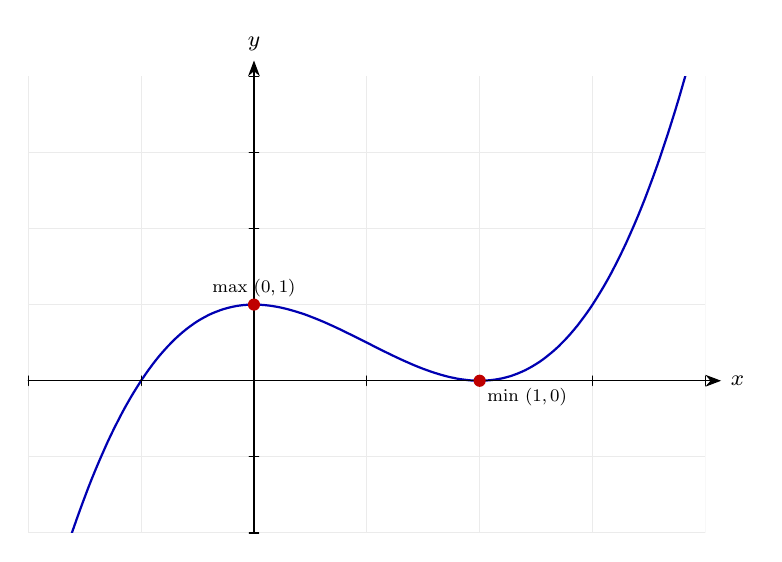
\begin{tikzpicture}[>={Stealth[length=2mm]},font=\footnotesize,line cap=round,line join=round]
\begin{scope}
\clip (0,0) rectangle (8.6,5.8);
\draw[gray!16] (0,0) grid[xstep=1.433,ystep=0.967] (8.6,5.8);
\draw[blue!70!black,thick] (0,-1.933) -- (0.048,-1.742) -- (0.096,-1.556) -- (0.143,-1.375) -- (0.191,-1.198) -- (0.239,-1.026) -- (0.287,-0.858) -- (0.334,-0.695) -- (0.382,-0.537) -- (0.43,-0.383) -- (0.478,-0.233) -- (0.526,-0.087) -- (0.573,0.054) -- (0.621,0.191) -- (0.669,0.324) -- (0.717,0.453) -- (0.764,0.578) -- (0.812,0.699) -- (0.86,0.816) -- (0.908,0.929) -- (0.956,1.038) -- (1.003,1.144) -- (1.051,1.246) -- (1.099,1.344) -- (1.147,1.438) -- (1.194,1.529) -- (1.242,1.617) -- (1.29,1.701) -- (1.338,1.782) -- (1.386,1.859) -- (1.433,1.933) -- (1.481,2.004) -- (1.529,2.072) -- (1.577,2.137) -- (1.624,2.198) -- (1.672,2.257) -- (1.72,2.312) -- (1.768,2.365) -- (1.816,2.415) -- (1.863,2.462) -- (1.911,2.506) -- (1.959,2.548) -- (2.007,2.587) -- (2.054,2.623) -- (2.102,2.657) -- (2.15,2.689) -- (2.198,2.718) -- (2.246,2.744) -- (2.293,2.769) -- (2.341,2.791) -- (2.389,2.81) -- (2.437,2.828) -- (2.484,2.844) -- (2.532,2.857) -- (2.58,2.869) -- (2.628,2.879) -- (2.676,2.887) -- (2.723,2.893) -- (2.771,2.897) -- (2.819,2.899) -- (2.867,2.9) -- (2.914,2.899) -- (2.962,2.897) -- (3.01,2.893) -- (3.058,2.888) -- (3.106,2.881) -- (3.153,2.873) -- (3.201,2.864) -- (3.249,2.853) -- (3.297,2.841) -- (3.344,2.828) -- (3.392,2.814) -- (3.44,2.799) -- (3.488,2.784) -- (3.536,2.767) -- (3.583,2.749) -- (3.631,2.73) -- (3.679,2.711) -- (3.727,2.691) -- (3.774,2.671) -- (3.822,2.649) -- (3.87,2.628) -- (3.918,2.605) -- (3.966,2.583) -- (4.013,2.56) -- (4.061,2.536) -- (4.109,2.513) -- (4.157,2.489) -- (4.204,2.465) -- (4.252,2.441) -- (4.3,2.417) -- (4.348,2.393) -- (4.396,2.368) -- (4.443,2.344) -- (4.491,2.321) -- (4.539,2.297) -- (4.587,2.274) -- (4.634,2.251) -- (4.682,2.228) -- (4.73,2.206) -- (4.778,2.184) -- (4.826,2.163) -- (4.873,2.142) -- (4.921,2.122) -- (4.969,2.103) -- (5.017,2.084) -- (5.064,2.067) -- (5.112,2.05) -- (5.16,2.034) -- (5.208,2.019) -- (5.256,2.005) -- (5.303,1.992) -- (5.351,1.98) -- (5.399,1.97) -- (5.447,1.96) -- (5.494,1.952) -- (5.542,1.946) -- (5.59,1.94) -- (5.638,1.936) -- (5.686,1.934) -- (5.733,1.933) -- (5.781,1.934) -- (5.829,1.937) -- (5.877,1.941) -- (5.924,1.947) -- (5.972,1.955) -- (6.02,1.964) -- (6.068,1.976) -- (6.116,1.989) -- (6.163,2.005) -- (6.211,2.023) -- (6.259,2.043) -- (6.307,2.065) -- (6.354,2.089) -- (6.402,2.116) -- (6.45,2.145) -- (6.498,2.176) -- (6.546,2.21) -- (6.593,2.247) -- (6.641,2.286) -- (6.689,2.327) -- (6.737,2.371) -- (6.784,2.419) -- (6.832,2.468) -- (6.88,2.521) -- (6.928,2.577) -- (6.976,2.635) -- (7.023,2.697) -- (7.071,2.761) -- (7.119,2.829) -- (7.167,2.9) -- (7.214,2.974) -- (7.262,3.052) -- (7.31,3.132) -- (7.358,3.216) -- (7.406,3.304) -- (7.453,3.395) -- (7.501,3.49) -- (7.549,3.588) -- (7.597,3.69) -- (7.644,3.795) -- (7.692,3.904) -- (7.74,4.017) -- (7.788,4.134) -- (7.836,4.255) -- (7.883,4.38) -- (7.931,4.509) -- (7.979,4.642) -- (8.027,4.779) -- (8.074,4.921) -- (8.122,5.066) -- (8.17,5.216) -- (8.218,5.37) -- (8.266,5.529) -- (8.313,5.692) -- (8.361,5.859) -- (8.409,6.031) -- (8.457,6.208) -- (8.504,6.39) -- (8.552,6.576) -- (8.6,6.767);
\end{scope}
\draw[->] (0,1.933) -- (8.8,1.933) node[right]{$x$};
\draw[->] (2.867,0) -- (2.867,6) node[above]{$y$};
\draw (0,1.873) -- (0,1.993);
\draw (1.433,1.873) -- (1.433,1.993);
\draw (4.3,1.873) -- (4.3,1.993);
\draw (5.733,1.873) -- (5.733,1.993);
\draw (7.167,1.873) -- (7.167,1.993);
\draw (8.6,1.873) -- (8.6,1.993);
\draw (2.807,0) -- (2.927,0);
\draw (2.807,0.967) -- (2.927,0.967);
\draw (2.807,2.9) -- (2.927,2.9);
\draw (2.807,3.867) -- (2.927,3.867);
\draw (2.807,4.833) -- (2.927,4.833);
\draw (2.807,5.8) -- (2.927,5.8);
\fill[red!75!black] (2.867,2.9) circle (2.2pt);
\node[above,scale=0.8] at (2.867,2.9) {max $(0,1)$};
\fill[red!75!black] (5.733,1.933) circle (2.2pt);
\node[below right,scale=0.8] at (5.733,1.933) {min $(1,0)$};
\end{tikzpicture}
}
\end{center}
\small Curve with classified stationary points marked.\normalsize

\medskip\hrule

\section*{Derivatives and Graphs 39\quad\small\texttt{(d4-039)}}
\addcontentsline{toc}{section}{Derivatives and Graphs 39 (d4-039)}
\textit{Difficulty: Standard \quad\textbar\quad Marks: 6}

\question{Find and classify the stationary points of \( y = 3x^4 - 8x^3 + 5 \).}

\textbf{Worked solution.}

\textit{Step 1: Differentiate.}
\[\begin{gathered}
\frac{\mathrm{d}y}{\mathrm{d}x} = 12x^3 - 24x^2 = 12x^2(x - 2)
\end{gathered}\]
Factor out \( 12x^2 \).

\textit{Step 2: Solve.}
\[\begin{gathered}
x = 0 \text{ (double root) or } x = 2
\end{gathered}\]
Two candidate stationary points.

\textit{Step 3: Find \( y \).}
\[\begin{gathered}
y(0) = 5,\; y(2) = 48 - 64 + 5 = -11
\end{gathered}\]
Substitute.

\textit{Step 4: Sign test near \( x = 0 \).}
\[\begin{gathered}
y'(-1) = -12 - 24 = -36 < 0,\; y'(0.5) = 1.5 - 6 = -4.5 < 0
\end{gathered}\]
No sign change at \( x = 0 \), so this is a stationary point of inflection.

\textit{Step 5: Sign test near \( x = 2 \).}
\[\begin{gathered}
y'(1) = 12 - 24 = -12 < 0,\; y'(3) = 324 - 216 = 108 > 0
\end{gathered}\]
Sign changes $-$ $\to$ +, so minimum.

\begin{answerbox}
\textbf{Final answer:}\quad Stationary point of inflection at \(\displaystyle  (0, 5) \); minimum at \(\displaystyle  (2, -11) \).
\end{answerbox}
\textbf{Diagram.}

\begin{center}
\resizebox{\ifdim\width>\linewidth \linewidth\else \width\fi}{!}{%
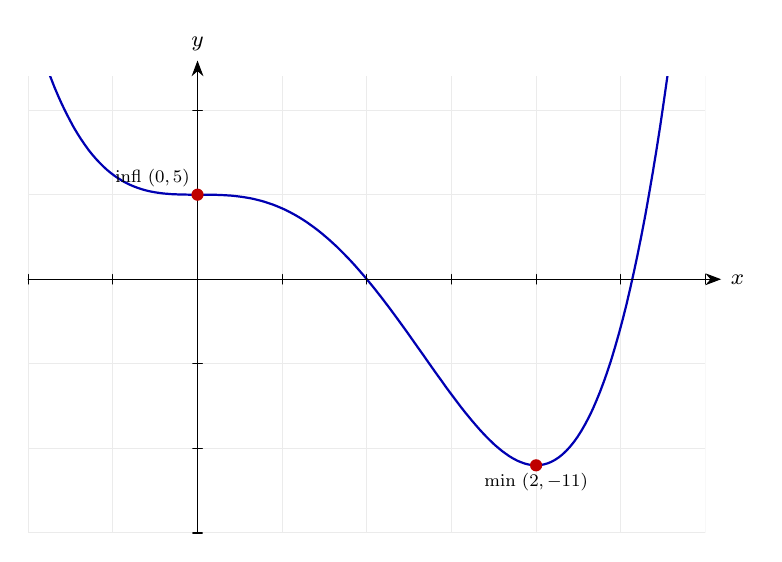
\begin{tikzpicture}[>={Stealth[length=2mm]},font=\footnotesize,line cap=round,line join=round]
\begin{scope}
\clip (0,0) rectangle (8.6,5.8);
\draw[gray!16] (0,0) grid[xstep=1.075,ystep=1.074] (8.6,5.8);
\draw[blue!70!black,thick] (0,6.659) -- (0.048,6.492) -- (0.096,6.333) -- (0.143,6.183) -- (0.191,6.04) -- (0.239,5.906) -- (0.287,5.779) -- (0.334,5.659) -- (0.382,5.546) -- (0.43,5.44) -- (0.478,5.341) -- (0.526,5.248) -- (0.573,5.16) -- (0.621,5.079) -- (0.669,5.003) -- (0.717,4.933) -- (0.764,4.867) -- (0.812,4.807) -- (0.86,4.751) -- (0.908,4.7) -- (0.956,4.652) -- (1.003,4.609) -- (1.051,4.57) -- (1.099,4.534) -- (1.147,4.502) -- (1.194,4.472) -- (1.242,4.446) -- (1.29,4.423) -- (1.338,4.402) -- (1.386,4.384) -- (1.433,4.368) -- (1.481,4.354) -- (1.529,4.342) -- (1.577,4.332) -- (1.624,4.324) -- (1.672,4.317) -- (1.72,4.311) -- (1.768,4.307) -- (1.816,4.303) -- (1.863,4.301) -- (1.911,4.299) -- (1.959,4.298) -- (2.007,4.297) -- (2.054,4.296) -- (2.102,4.296) -- (2.15,4.296) -- (2.198,4.296) -- (2.246,4.296) -- (2.293,4.296) -- (2.341,4.295) -- (2.389,4.294) -- (2.437,4.292) -- (2.484,4.29) -- (2.532,4.287) -- (2.58,4.284) -- (2.628,4.279) -- (2.676,4.273) -- (2.723,4.267) -- (2.771,4.259) -- (2.819,4.251) -- (2.867,4.241) -- (2.914,4.229) -- (2.962,4.217) -- (3.01,4.203) -- (3.058,4.187) -- (3.106,4.171) -- (3.153,4.152) -- (3.201,4.132) -- (3.249,4.111) -- (3.297,4.088) -- (3.344,4.063) -- (3.392,4.037) -- (3.44,4.009) -- (3.488,3.979) -- (3.536,3.948) -- (3.583,3.914) -- (3.631,3.88) -- (3.679,3.843) -- (3.727,3.805) -- (3.774,3.765) -- (3.822,3.724) -- (3.87,3.68) -- (3.918,3.636) -- (3.966,3.589) -- (4.013,3.541) -- (4.061,3.492) -- (4.109,3.441) -- (4.157,3.388) -- (4.204,3.334) -- (4.252,3.279) -- (4.3,3.222) -- (4.348,3.164) -- (4.396,3.105) -- (4.443,3.045) -- (4.491,2.984) -- (4.539,2.921) -- (4.587,2.858) -- (4.634,2.794) -- (4.682,2.729) -- (4.73,2.663) -- (4.778,2.597) -- (4.826,2.53) -- (4.873,2.463) -- (4.921,2.395) -- (4.969,2.327) -- (5.017,2.26) -- (5.064,2.192) -- (5.112,2.124) -- (5.16,2.056) -- (5.208,1.989) -- (5.256,1.923) -- (5.303,1.856) -- (5.351,1.791) -- (5.399,1.727) -- (5.447,1.663) -- (5.494,1.601) -- (5.542,1.54) -- (5.59,1.481) -- (5.638,1.423) -- (5.686,1.367) -- (5.733,1.313) -- (5.781,1.261) -- (5.829,1.211) -- (5.877,1.164) -- (5.924,1.119) -- (5.972,1.078) -- (6.02,1.039) -- (6.068,1.004) -- (6.116,0.971) -- (6.163,0.943) -- (6.211,0.918) -- (6.259,0.898) -- (6.307,0.881) -- (6.354,0.869) -- (6.402,0.862) -- (6.45,0.859) -- (6.498,0.862) -- (6.546,0.87) -- (6.593,0.883) -- (6.641,0.902) -- (6.689,0.928) -- (6.737,0.959) -- (6.784,0.997) -- (6.832,1.042) -- (6.88,1.094) -- (6.928,1.153) -- (6.976,1.22) -- (7.023,1.294) -- (7.071,1.377) -- (7.119,1.468) -- (7.167,1.567) -- (7.214,1.676) -- (7.262,1.793) -- (7.31,1.921) -- (7.358,2.058) -- (7.406,2.205) -- (7.453,2.362) -- (7.501,2.53) -- (7.549,2.709) -- (7.597,2.899) -- (7.644,3.101) -- (7.692,3.315) -- (7.74,3.541) -- (7.788,3.78) -- (7.836,4.031) -- (7.883,4.296) -- (7.931,4.575) -- (7.979,4.867) -- (8.027,5.174) -- (8.074,5.495) -- (8.122,5.831) -- (8.17,6.183) -- (8.218,6.55) -- (8.266,6.933) -- (8.313,7.333) -- (8.361,7.749) -- (8.409,8.183) -- (8.457,8.634) -- (8.504,9.103) -- (8.552,9.59) -- (8.6,10.096);
\end{scope}
\draw[->] (0,3.222) -- (8.8,3.222) node[right]{$x$};
\draw[->] (2.15,0) -- (2.15,6) node[above]{$y$};
\draw (0,3.162) -- (0,3.282);
\draw (1.075,3.162) -- (1.075,3.282);
\draw (3.225,3.162) -- (3.225,3.282);
\draw (4.3,3.162) -- (4.3,3.282);
\draw (5.375,3.162) -- (5.375,3.282);
\draw (6.45,3.162) -- (6.45,3.282);
\draw (7.525,3.162) -- (7.525,3.282);
\draw (8.6,3.162) -- (8.6,3.282);
\draw (2.09,0) -- (2.21,0);
\draw (2.09,1.074) -- (2.21,1.074);
\draw (2.09,2.148) -- (2.21,2.148);
\draw (2.09,4.296) -- (2.21,4.296);
\draw (2.09,5.37) -- (2.21,5.37);
\fill[red!75!black] (2.15,4.296) circle (2.2pt);
\node[above left,scale=0.8] at (2.15,4.296) {infl $(0,5)$};
\fill[red!75!black] (6.45,0.859) circle (2.2pt);
\node[below,scale=0.8] at (6.45,0.859) {min $(2,-11)$};
\end{tikzpicture}
}
\end{center}
\small Curve with classified stationary points marked.\normalsize

\medskip\hrule

\section*{Derivatives and Graphs 40\quad\small\texttt{(d4-040)}}
\addcontentsline{toc}{section}{Derivatives and Graphs 40 (d4-040)}
\textit{Difficulty: Standard \quad\textbar\quad Marks: 5}

\question{Find the stationary points of \( f(x) = x^3 - 6x^2 + 12x - 3 \) and determine their nature.}

\textbf{Worked solution.}

\textit{Step 1: Differentiate.}
\[\begin{gathered}
f'(x) = 3x^2 - 12x + 12 = 3(x - 2)^2
\end{gathered}\]
Complete the square after factoring 3.

\textit{Step 2: Set to zero.}
\[\begin{gathered}
(x - 2)^2 = 0 \Rightarrow x = 2
\end{gathered}\]
Repeated root.

\textit{Step 3: Find \( y \).}
\[\begin{gathered}
f(2) = 8 - 24 + 24 - 3 = 5
\end{gathered}\]
Substitute.

\textit{Step 4: Sign of \( f'(x) \) around \( x = 2 \).}
\[\begin{gathered}
f'(1) = 3 > 0,\; f'(3) = 3 > 0
\end{gathered}\]
No change of sign, so stationary point of inflection.

\begin{answerbox}
\textbf{Final answer:}\quad Stationary point of inflection at \(\displaystyle  (2, 5) \).
\end{answerbox}
\textbf{Diagram.}

\begin{center}
\resizebox{\ifdim\width>\linewidth \linewidth\else \width\fi}{!}{%
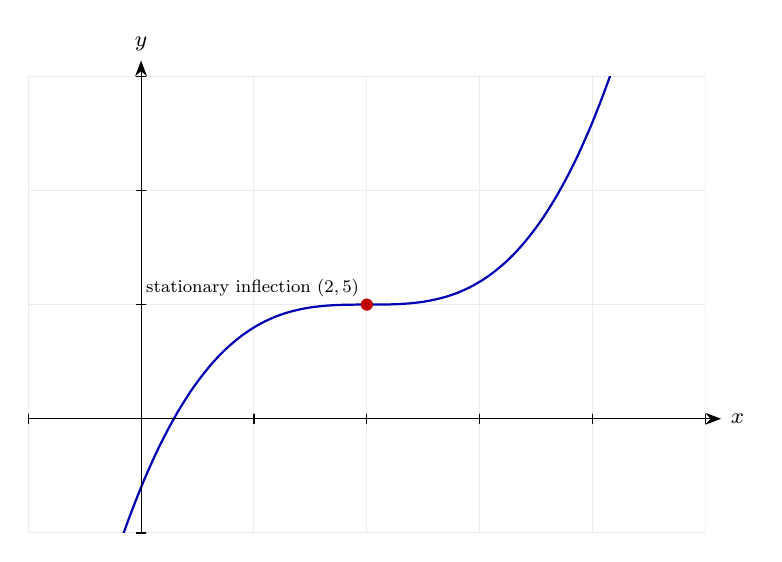
\begin{tikzpicture}[>={Stealth[length=2mm]},font=\footnotesize,line cap=round,line join=round]
\begin{scope}
\clip (0,0) rectangle (8.6,5.8);
\draw[gray!16] (0,0) grid[xstep=1.433,ystep=1.45] (8.6,5.8);
\draw[blue!70!black,thick] (0,-4.93) -- (0.048,-4.672) -- (0.096,-4.42) -- (0.143,-4.173) -- (0.191,-3.932) -- (0.239,-3.696) -- (0.287,-3.466) -- (0.334,-3.241) -- (0.382,-3.022) -- (0.43,-2.808) -- (0.478,-2.599) -- (0.526,-2.396) -- (0.573,-2.197) -- (0.621,-2.004) -- (0.669,-1.815) -- (0.717,-1.631) -- (0.764,-1.452) -- (0.812,-1.278) -- (0.86,-1.109) -- (0.908,-0.944) -- (0.956,-0.784) -- (1.003,-0.628) -- (1.051,-0.477) -- (1.099,-0.33) -- (1.147,-0.188) -- (1.194,-0.05) -- (1.242,0.084) -- (1.29,0.214) -- (1.338,0.34) -- (1.386,0.462) -- (1.433,0.58) -- (1.481,0.694) -- (1.529,0.804) -- (1.577,0.911) -- (1.624,1.014) -- (1.672,1.113) -- (1.72,1.209) -- (1.768,1.301) -- (1.816,1.39) -- (1.863,1.475) -- (1.911,1.557) -- (1.959,1.636) -- (2.007,1.712) -- (2.054,1.785) -- (2.102,1.855) -- (2.15,1.921) -- (2.198,1.985) -- (2.246,2.046) -- (2.293,2.104) -- (2.341,2.16) -- (2.389,2.213) -- (2.437,2.263) -- (2.484,2.311) -- (2.532,2.356) -- (2.58,2.399) -- (2.628,2.439) -- (2.676,2.478) -- (2.723,2.514) -- (2.771,2.548) -- (2.819,2.58) -- (2.867,2.61) -- (2.914,2.638) -- (2.962,2.664) -- (3.01,2.689) -- (3.058,2.711) -- (3.106,2.732) -- (3.153,2.752) -- (3.201,2.769) -- (3.249,2.786) -- (3.297,2.801) -- (3.344,2.814) -- (3.392,2.826) -- (3.44,2.837) -- (3.488,2.847) -- (3.536,2.856) -- (3.583,2.864) -- (3.631,2.871) -- (3.679,2.876) -- (3.727,2.881) -- (3.774,2.886) -- (3.822,2.889) -- (3.87,2.892) -- (3.918,2.895) -- (3.966,2.896) -- (4.013,2.898) -- (4.061,2.899) -- (4.109,2.899) -- (4.157,2.9) -- (4.204,2.9) -- (4.252,2.9) -- (4.3,2.9) -- (4.348,2.9) -- (4.396,2.9) -- (4.443,2.9) -- (4.491,2.901) -- (4.539,2.901) -- (4.587,2.902) -- (4.634,2.904) -- (4.682,2.905) -- (4.73,2.908) -- (4.778,2.911) -- (4.826,2.914) -- (4.873,2.919) -- (4.921,2.924) -- (4.969,2.929) -- (5.017,2.936) -- (5.064,2.944) -- (5.112,2.953) -- (5.16,2.963) -- (5.208,2.974) -- (5.256,2.986) -- (5.303,2.999) -- (5.351,3.014) -- (5.399,3.031) -- (5.447,3.048) -- (5.494,3.068) -- (5.542,3.089) -- (5.59,3.111) -- (5.638,3.136) -- (5.686,3.162) -- (5.733,3.19) -- (5.781,3.22) -- (5.829,3.252) -- (5.877,3.286) -- (5.924,3.322) -- (5.972,3.361) -- (6.02,3.401) -- (6.068,3.444) -- (6.116,3.489) -- (6.163,3.537) -- (6.211,3.587) -- (6.259,3.64) -- (6.307,3.696) -- (6.354,3.754) -- (6.402,3.815) -- (6.45,3.879) -- (6.498,3.945) -- (6.546,4.015) -- (6.593,4.088) -- (6.641,4.164) -- (6.689,4.243) -- (6.737,4.325) -- (6.784,4.41) -- (6.832,4.499) -- (6.88,4.591) -- (6.928,4.687) -- (6.976,4.786) -- (7.023,4.889) -- (7.071,4.996) -- (7.119,5.106) -- (7.167,5.22) -- (7.214,5.338) -- (7.262,5.46) -- (7.31,5.586) -- (7.358,5.716) -- (7.406,5.85) -- (7.453,5.988) -- (7.501,6.13) -- (7.549,6.277) -- (7.597,6.428) -- (7.644,6.584) -- (7.692,6.744) -- (7.74,6.909) -- (7.788,7.078) -- (7.836,7.252) -- (7.883,7.431) -- (7.931,7.615) -- (7.979,7.804) -- (8.027,7.997) -- (8.074,8.196) -- (8.122,8.399) -- (8.17,8.608) -- (8.218,8.822) -- (8.266,9.041) -- (8.313,9.266) -- (8.361,9.496) -- (8.409,9.732) -- (8.457,9.973) -- (8.504,10.22) -- (8.552,10.472) -- (8.6,10.73);
\end{scope}
\draw[->] (0,1.45) -- (8.8,1.45) node[right]{$x$};
\draw[->] (1.433,0) -- (1.433,6) node[above]{$y$};
\draw (0,1.39) -- (0,1.51);
\draw (2.867,1.39) -- (2.867,1.51);
\draw (4.3,1.39) -- (4.3,1.51);
\draw (5.733,1.39) -- (5.733,1.51);
\draw (7.167,1.39) -- (7.167,1.51);
\draw (8.6,1.39) -- (8.6,1.51);
\draw (1.373,0) -- (1.493,0);
\draw (1.373,2.9) -- (1.493,2.9);
\draw (1.373,4.35) -- (1.493,4.35);
\draw (1.373,5.8) -- (1.493,5.8);
\fill[red!75!black] (4.3,2.9) circle (2.2pt);
\node[above left,scale=0.8] at (4.3,2.9) {stationary inflection $(2,5)$};
\end{tikzpicture}
}
\end{center}
\small Curve with classified stationary points marked.\normalsize

\medskip\hrule

\section*{Derivatives and Graphs 41\quad\small\texttt{(d4-041)}}
\addcontentsline{toc}{section}{Derivatives and Graphs 41 (d4-041)}
\textit{Difficulty: Standard \quad\textbar\quad Marks: 6}

\question{Find the stationary points of \( y = x(x - 4)^2 \) and classify them.}

\textbf{Worked solution.}

\textit{Step 1: Expand.}
\[\begin{gathered}
y = x(x^2 - 8x + 16) = x^3 - 8x^2 + 16x
\end{gathered}\]
Prepare to differentiate.

\textit{Step 2: Differentiate.}
\[\begin{gathered}
\frac{\mathrm{d}y}{\mathrm{d}x} = 3x^2 - 16x + 16
\end{gathered}\]
Apply the power rule.

\textit{Step 3: Factorise.}
\[\begin{gathered}
(3x - 4)(x - 4) = 0 \Rightarrow x = \tfrac{4}{3} \text{ or } x = 4
\end{gathered}\]
Split into two factors.

\textit{Step 4: Find \( y \).}
\[\begin{gathered}
y\!\left(\tfrac{4}{3}\right) = \tfrac{4}{3} \cdot \tfrac{64}{9} = \tfrac{256}{27} \\ y(4) = 0
\end{gathered}\]
Substitute back.

\textit{Step 5: Second derivative test.}
\[\begin{gathered}
y'' = 6x - 16 \\ y''(\tfrac{4}{3}) = 8 - 16 = -8 < 0\; (\text{max}) \\ y''(4) = 24 - 16 = 8 > 0\; (\text{min})
\end{gathered}\]
Classify each.

\begin{answerbox}
\textbf{Final answer:}\quad Maximum at \(\displaystyle  (\tfrac{4}{3}, \tfrac{256}{27}) \); minimum at \(\displaystyle  (4, 0) \).
\end{answerbox}
\textbf{Diagram.}

\begin{center}
\resizebox{\ifdim\width>\linewidth \linewidth\else \width\fi}{!}{%
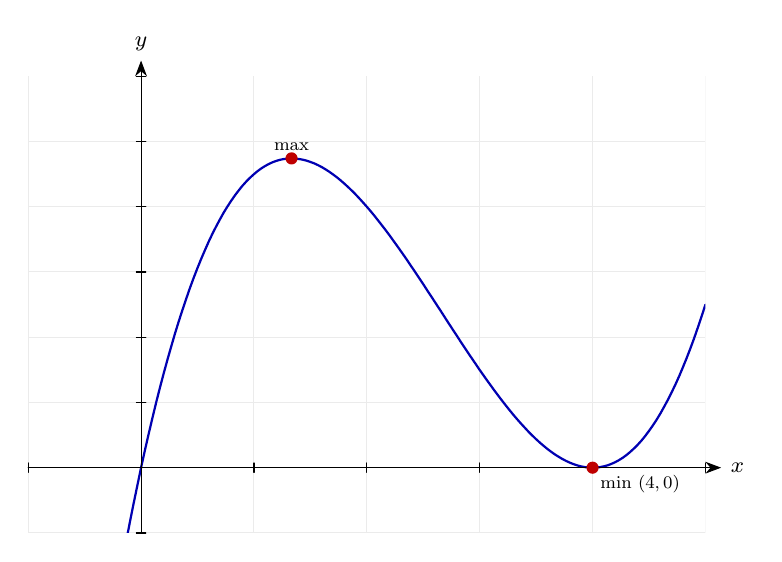
\begin{tikzpicture}[>={Stealth[length=2mm]},font=\footnotesize,line cap=round,line join=round]
\begin{scope}
\clip (0,0) rectangle (8.6,5.8);
\draw[gray!16] (0,0) grid[xstep=1.433,ystep=0.829] (8.6,5.8);
\draw[blue!70!black,thick] (0,-5.8) -- (0.048,-5.8) -- (0.096,-5.8) -- (0.143,-5.8) -- (0.191,-5.8) -- (0.239,-5.8) -- (0.287,-5.8) -- (0.334,-5.8) -- (0.382,-5.8) -- (0.43,-5.578) -- (0.478,-5.186) -- (0.526,-4.804) -- (0.573,-4.431) -- (0.621,-4.067) -- (0.669,-3.712) -- (0.717,-3.366) -- (0.764,-3.029) -- (0.812,-2.7) -- (0.86,-2.38) -- (0.908,-2.068) -- (0.956,-1.765) -- (1.003,-1.469) -- (1.051,-1.183) -- (1.099,-0.904) -- (1.147,-0.633) -- (1.194,-0.37) -- (1.242,-0.115) -- (1.29,0.132) -- (1.338,0.372) -- (1.386,0.604) -- (1.433,0.829) -- (1.481,1.046) -- (1.529,1.256) -- (1.577,1.459) -- (1.624,1.654) -- (1.672,1.843) -- (1.72,2.025) -- (1.768,2.2) -- (1.816,2.368) -- (1.863,2.53) -- (1.911,2.685) -- (1.959,2.834) -- (2.007,2.976) -- (2.054,3.112) -- (2.102,3.242) -- (2.15,3.366) -- (2.198,3.484) -- (2.246,3.596) -- (2.293,3.702) -- (2.341,3.803) -- (2.389,3.897) -- (2.437,3.987) -- (2.484,4.071) -- (2.532,4.149) -- (2.58,4.222) -- (2.628,4.291) -- (2.676,4.354) -- (2.723,4.412) -- (2.771,4.465) -- (2.819,4.513) -- (2.867,4.557) -- (2.914,4.596) -- (2.962,4.631) -- (3.01,4.661) -- (3.058,4.687) -- (3.106,4.709) -- (3.153,4.726) -- (3.201,4.74) -- (3.249,4.749) -- (3.297,4.755) -- (3.344,4.757) -- (3.392,4.755) -- (3.44,4.749) -- (3.488,4.74) -- (3.536,4.728) -- (3.583,4.712) -- (3.631,4.694) -- (3.679,4.672) -- (3.727,4.647) -- (3.774,4.619) -- (3.822,4.588) -- (3.87,4.554) -- (3.918,4.518) -- (3.966,4.479) -- (4.013,4.438) -- (4.061,4.394) -- (4.109,4.348) -- (4.157,4.3) -- (4.204,4.25) -- (4.252,4.197) -- (4.3,4.143) -- (4.348,4.087) -- (4.396,4.029) -- (4.443,3.969) -- (4.491,3.908) -- (4.539,3.846) -- (4.587,3.782) -- (4.634,3.716) -- (4.682,3.65) -- (4.73,3.582) -- (4.778,3.514) -- (4.826,3.444) -- (4.873,3.374) -- (4.921,3.303) -- (4.969,3.231) -- (5.017,3.159) -- (5.064,3.086) -- (5.112,3.013) -- (5.16,2.94) -- (5.208,2.866) -- (5.256,2.793) -- (5.303,2.719) -- (5.351,2.645) -- (5.399,2.572) -- (5.447,2.499) -- (5.494,2.426) -- (5.542,2.354) -- (5.59,2.282) -- (5.638,2.211) -- (5.686,2.141) -- (5.733,2.071) -- (5.781,2.003) -- (5.829,1.935) -- (5.877,1.869) -- (5.924,1.804) -- (5.972,1.74) -- (6.02,1.677) -- (6.068,1.616) -- (6.116,1.556) -- (6.163,1.498) -- (6.211,1.442) -- (6.259,1.388) -- (6.307,1.336) -- (6.354,1.285) -- (6.402,1.237) -- (6.45,1.191) -- (6.498,1.147) -- (6.546,1.106) -- (6.593,1.067) -- (6.641,1.031) -- (6.689,0.997) -- (6.737,0.967) -- (6.784,0.939) -- (6.832,0.914) -- (6.88,0.892) -- (6.928,0.873) -- (6.976,0.857) -- (7.023,0.845) -- (7.071,0.836) -- (7.119,0.83) -- (7.167,0.829) -- (7.214,0.83) -- (7.262,0.836) -- (7.31,0.846) -- (7.358,0.859) -- (7.406,0.877) -- (7.453,0.898) -- (7.501,0.924) -- (7.549,0.954) -- (7.597,0.989) -- (7.644,1.028) -- (7.692,1.072) -- (7.74,1.12) -- (7.788,1.173) -- (7.836,1.232) -- (7.883,1.295) -- (7.931,1.363) -- (7.979,1.436) -- (8.027,1.515) -- (8.074,1.599) -- (8.122,1.688) -- (8.17,1.783) -- (8.218,1.883) -- (8.266,1.989) -- (8.313,2.101) -- (8.361,2.219) -- (8.409,2.343) -- (8.457,2.473) -- (8.504,2.609) -- (8.552,2.751) -- (8.6,2.9);
\end{scope}
\draw[->] (0,0.829) -- (8.8,0.829) node[right]{$x$};
\draw[->] (1.433,0) -- (1.433,6) node[above]{$y$};
\draw (0,0.769) -- (0,0.889);
\draw (2.867,0.769) -- (2.867,0.889);
\draw (4.3,0.769) -- (4.3,0.889);
\draw (5.733,0.769) -- (5.733,0.889);
\draw (7.167,0.769) -- (7.167,0.889);
\draw (8.6,0.769) -- (8.6,0.889);
\draw (1.373,0) -- (1.493,0);
\draw (1.373,1.657) -- (1.493,1.657);
\draw (1.373,2.486) -- (1.493,2.486);
\draw (1.373,3.314) -- (1.493,3.314);
\draw (1.373,4.143) -- (1.493,4.143);
\draw (1.373,4.971) -- (1.493,4.971);
\draw (1.373,5.8) -- (1.493,5.8);
\fill[red!75!black] (3.344,4.757) circle (2.2pt);
\node[above,scale=0.8] at (3.344,4.757) {max};
\fill[red!75!black] (7.167,0.829) circle (2.2pt);
\node[below right,scale=0.8] at (7.167,0.829) {min $(4,0)$};
\end{tikzpicture}
}
\end{center}
\small Curve with classified stationary points marked.\normalsize

\medskip\hrule

\section*{Derivatives and Graphs 42\quad\small\texttt{(d4-042)}}
\addcontentsline{toc}{section}{Derivatives and Graphs 42 (d4-042)}
\textit{Difficulty: Standard \quad\textbar\quad Marks: 5}

\question{A curve has equation \( y = x^3 - 3x^2 + 3x + 2 \). Show that the curve has no turning points and state the nature of any stationary points.}

\textbf{Worked solution.}

\textit{Step 1: Differentiate.}
\[\begin{gathered}
\frac{\mathrm{d}y}{\mathrm{d}x} = 3x^2 - 6x + 3
\end{gathered}\]
Apply the power rule.

\textit{Step 2: Factorise.}
\[\begin{gathered}
3(x - 1)^2
\end{gathered}\]
A perfect square.

\textit{Step 3: Stationary at \( x = 1 \), but gradient \( \geq 0 \) everywhere.}
\[\begin{gathered}
3(x-1)^2 \geq 0 \; \text{for all } x
\end{gathered}\]
The derivative is never negative, so there are no turning points.

\textit{Step 4: Nature at \( x = 1 \).}
\[\begin{gathered}
y(1) = 1 - 3 + 3 + 2 = 3
\end{gathered}\]
Since \( y' \) doesn't change sign, \( (1, 3) \) is a stationary point of inflection.

\begin{answerbox}
\textbf{Final answer:}\quad No turning points --- stationary point of inflection at \(\displaystyle  (1, 3) \).
\end{answerbox}
\textbf{Diagram.}

\begin{center}
\resizebox{\ifdim\width>\linewidth \linewidth\else \width\fi}{!}{%
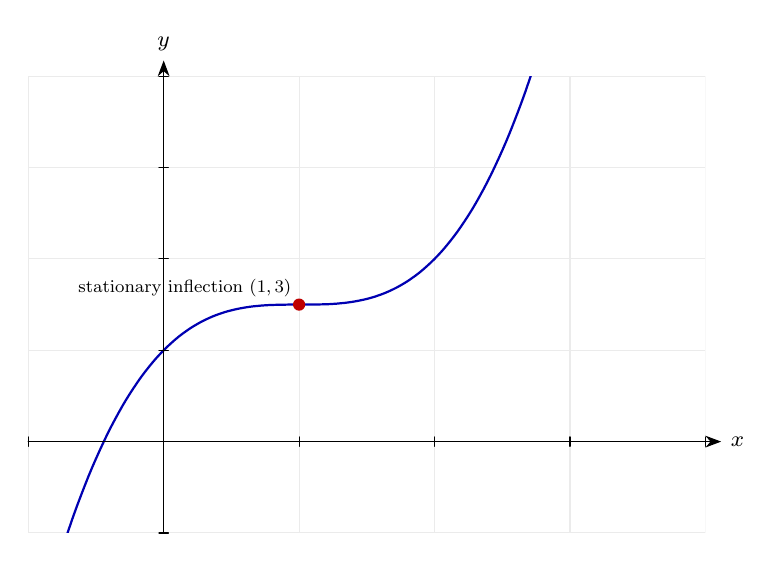
\begin{tikzpicture}[>={Stealth[length=2mm]},font=\footnotesize,line cap=round,line join=round]
\begin{scope}
\clip (0,0) rectangle (8.6,5.8);
\draw[gray!16] (0,0) grid[xstep=1.72,ystep=1.16] (8.6,5.8);
\draw[blue!70!black,thick] (0,-1.74) -- (0.048,-1.549) -- (0.096,-1.364) -- (0.143,-1.184) -- (0.191,-1.009) -- (0.239,-0.839) -- (0.287,-0.674) -- (0.334,-0.514) -- (0.382,-0.359) -- (0.43,-0.208) -- (0.478,-0.063) -- (0.526,0.078) -- (0.573,0.215) -- (0.621,0.347) -- (0.669,0.474) -- (0.717,0.598) -- (0.764,0.717) -- (0.812,0.832) -- (0.86,0.942) -- (0.908,1.049) -- (0.956,1.152) -- (1.003,1.251) -- (1.051,1.346) -- (1.099,1.437) -- (1.147,1.525) -- (1.194,1.609) -- (1.242,1.69) -- (1.29,1.767) -- (1.338,1.841) -- (1.386,1.912) -- (1.433,1.979) -- (1.481,2.043) -- (1.529,2.104) -- (1.577,2.163) -- (1.624,2.218) -- (1.672,2.27) -- (1.72,2.32) -- (1.768,2.367) -- (1.816,2.411) -- (1.863,2.453) -- (1.911,2.493) -- (1.959,2.53) -- (2.007,2.564) -- (2.054,2.597) -- (2.102,2.627) -- (2.15,2.655) -- (2.198,2.682) -- (2.246,2.706) -- (2.293,2.728) -- (2.341,2.749) -- (2.389,2.768) -- (2.437,2.785) -- (2.484,2.801) -- (2.532,2.815) -- (2.58,2.827) -- (2.628,2.839) -- (2.676,2.849) -- (2.723,2.858) -- (2.771,2.866) -- (2.819,2.873) -- (2.867,2.879) -- (2.914,2.883) -- (2.962,2.888) -- (3.01,2.891) -- (3.058,2.894) -- (3.106,2.896) -- (3.153,2.897) -- (3.201,2.898) -- (3.249,2.899) -- (3.297,2.9) -- (3.344,2.9) -- (3.392,2.9) -- (3.44,2.9) -- (3.488,2.9) -- (3.536,2.9) -- (3.583,2.9) -- (3.631,2.901) -- (3.679,2.902) -- (3.727,2.903) -- (3.774,2.904) -- (3.822,2.906) -- (3.87,2.909) -- (3.918,2.912) -- (3.966,2.917) -- (4.013,2.921) -- (4.061,2.927) -- (4.109,2.934) -- (4.157,2.942) -- (4.204,2.951) -- (4.252,2.961) -- (4.3,2.972) -- (4.348,2.985) -- (4.396,2.999) -- (4.443,3.015) -- (4.491,3.032) -- (4.539,3.051) -- (4.587,3.072) -- (4.634,3.094) -- (4.682,3.118) -- (4.73,3.145) -- (4.778,3.173) -- (4.826,3.203) -- (4.873,3.236) -- (4.921,3.27) -- (4.969,3.307) -- (5.017,3.347) -- (5.064,3.389) -- (5.112,3.433) -- (5.16,3.48) -- (5.208,3.53) -- (5.256,3.582) -- (5.303,3.637) -- (5.351,3.696) -- (5.399,3.757) -- (5.447,3.821) -- (5.494,3.888) -- (5.542,3.959) -- (5.59,4.033) -- (5.638,4.11) -- (5.686,4.191) -- (5.733,4.275) -- (5.781,4.363) -- (5.829,4.454) -- (5.877,4.549) -- (5.924,4.648) -- (5.972,4.751) -- (6.02,4.857) -- (6.068,4.968) -- (6.116,5.083) -- (6.163,5.202) -- (6.211,5.326) -- (6.259,5.453) -- (6.307,5.585) -- (6.354,5.722) -- (6.402,5.863) -- (6.45,6.008) -- (6.498,6.159) -- (6.546,6.314) -- (6.593,6.474) -- (6.641,6.639) -- (6.689,6.809) -- (6.737,6.984) -- (6.784,7.164) -- (6.832,7.349) -- (6.88,7.54) -- (6.928,7.736) -- (6.976,7.938) -- (7.023,8.145) -- (7.071,8.357) -- (7.119,8.575) -- (7.167,8.799) -- (7.214,9.029) -- (7.262,9.265) -- (7.31,9.507) -- (7.358,9.754) -- (7.406,10.008) -- (7.453,10.268) -- (7.501,10.534) -- (7.549,10.807) -- (7.597,11.086) -- (7.644,11.372) -- (7.692,11.6) -- (7.74,11.6) -- (7.788,11.6) -- (7.836,11.6) -- (7.883,11.6) -- (7.931,11.6) -- (7.979,11.6) -- (8.027,11.6) -- (8.074,11.6) -- (8.122,11.6) -- (8.17,11.6) -- (8.218,11.6) -- (8.266,11.6) -- (8.313,11.6) -- (8.361,11.6) -- (8.409,11.6) -- (8.457,11.6) -- (8.504,11.6) -- (8.552,11.6) -- (8.6,11.6);
\end{scope}
\draw[->] (0,1.16) -- (8.8,1.16) node[right]{$x$};
\draw[->] (1.72,0) -- (1.72,6) node[above]{$y$};
\draw (0,1.1) -- (0,1.22);
\draw (3.44,1.1) -- (3.44,1.22);
\draw (5.16,1.1) -- (5.16,1.22);
\draw (6.88,1.1) -- (6.88,1.22);
\draw (8.6,1.1) -- (8.6,1.22);
\draw (1.66,0) -- (1.78,0);
\draw (1.66,2.32) -- (1.78,2.32);
\draw (1.66,3.48) -- (1.78,3.48);
\draw (1.66,4.64) -- (1.78,4.64);
\draw (1.66,5.8) -- (1.78,5.8);
\fill[red!75!black] (3.44,2.9) circle (2.2pt);
\node[above left,scale=0.8] at (3.44,2.9) {stationary inflection $(1,3)$};
\end{tikzpicture}
}
\end{center}
\small Curve with classified stationary points marked.\normalsize

\medskip\hrule

\section*{Derivatives and Graphs 43\quad\small\texttt{(d4-043)}}
\addcontentsline{toc}{section}{Derivatives and Graphs 43 (d4-043)}
\textit{Difficulty: Standard \quad\textbar\quad Marks: 5}

\question{Find the range of values of \( x \) for which \( f(x) = x^4 - 2x^2 \) is increasing.}

\textbf{Worked solution.}

\textit{Step 1: Differentiate.}
\[\begin{gathered}
f'(x) = 4x^3 - 4x = 4x(x - 1)(x + 1)
\end{gathered}\]
Factor out \( 4x \), then factorise the difference of squares.

\textit{Step 2: Find where \( f'(x) > 0 \).}
\[\begin{gathered}
4x(x - 1)(x + 1) > 0
\end{gathered}\]
Solve using a sign table for three roots at \( -1, 0, 1 \).

\textit{Step 3: Sign analysis.}
\[\begin{gathered}
x < -1: \; (+)(-)(-)(-) \Rightarrow - \\ -1 < x < 0: \; (+)(-)(-)(+) \Rightarrow + \\ 0 < x < 1: \; (+)(+)(-)(+) \Rightarrow - \\ x > 1: \; (+)(+)(+)(+) \Rightarrow +
\end{gathered}\]
Track sign on each interval.

\begin{answerbox}
\textbf{Final answer:}\quad Increasing on \(\displaystyle  -1 < x < 0 \) and \(\displaystyle  x > 1 \).
\end{answerbox}
\textbf{Diagram.}

\begin{center}
\resizebox{\ifdim\width>\linewidth \linewidth\else \width\fi}{!}{%
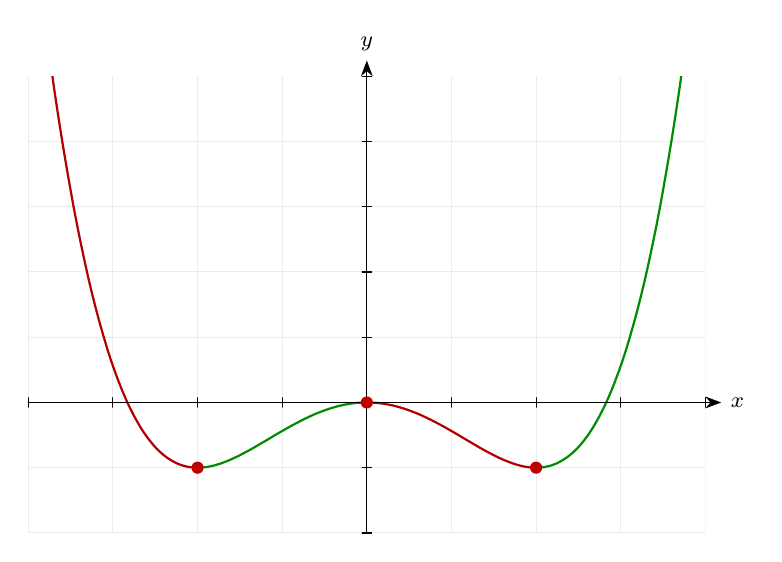
\begin{tikzpicture}[>={Stealth[length=2mm]},font=\footnotesize,line cap=round,line join=round]
\begin{scope}
\clip (0,0) rectangle (8.6,5.8);
\draw[gray!16] (0,0) grid[xstep=1.075,ystep=0.829] (8.6,5.8);
\draw[red!70!black,thick] (0,8.286) -- (0.048,7.853) -- (0.096,7.437) -- (0.143,7.039) -- (0.191,6.658) -- (0.239,6.292) -- (0.287,5.943) -- (0.334,5.609) -- (0.382,5.29) -- (0.43,4.986) -- (0.478,4.696) -- (0.526,4.42) -- (0.573,4.158) -- (0.621,3.908) -- (0.669,3.672) -- (0.717,3.447) -- (0.764,3.235) -- (0.812,3.034) -- (0.86,2.845) -- (0.908,2.667) -- (0.956,2.499) -- (1.003,2.341) -- (1.051,2.193) -- (1.099,2.055) -- (1.147,1.926) -- (1.194,1.807) -- (1.242,1.695) -- (1.29,1.592) -- (1.338,1.497) -- (1.386,1.41) -- (1.433,1.33) -- (1.481,1.257) -- (1.529,1.191) -- (1.577,1.131) -- (1.624,1.078) -- (1.672,1.031) -- (1.72,0.989) -- (1.768,0.953) -- (1.816,0.922) -- (1.863,0.896) -- (1.911,0.874) -- (1.959,0.857) -- (2.007,0.844) -- (2.054,0.835) -- (2.102,0.83) -- (2.15,0.829);
\draw[green!55!black,thick] (2.15,0.829) -- (2.198,0.83) -- (2.246,0.835) -- (2.293,0.842) -- (2.341,0.852) -- (2.389,0.865) -- (2.437,0.88) -- (2.484,0.897) -- (2.532,0.916) -- (2.58,0.936) -- (2.628,0.958) -- (2.676,0.981) -- (2.723,1.006) -- (2.771,1.031) -- (2.819,1.057) -- (2.867,1.084) -- (2.914,1.112) -- (2.962,1.14) -- (3.01,1.168) -- (3.058,1.196) -- (3.106,1.225) -- (3.153,1.253) -- (3.201,1.281) -- (3.249,1.308) -- (3.297,1.336) -- (3.344,1.362) -- (3.392,1.388) -- (3.44,1.413) -- (3.488,1.438) -- (3.536,1.461) -- (3.583,1.483) -- (3.631,1.505) -- (3.679,1.525) -- (3.727,1.543) -- (3.774,1.561) -- (3.822,1.577) -- (3.87,1.592) -- (3.918,1.606) -- (3.966,1.618) -- (4.013,1.628) -- (4.061,1.637) -- (4.109,1.644) -- (4.157,1.65) -- (4.204,1.654) -- (4.252,1.656) -- (4.3,1.657);
\draw[red!70!black,thick] (4.3,1.657) -- (4.348,1.656) -- (4.396,1.654) -- (4.443,1.65) -- (4.491,1.644) -- (4.539,1.637) -- (4.587,1.628) -- (4.634,1.618) -- (4.682,1.606) -- (4.73,1.592) -- (4.778,1.577) -- (4.826,1.561) -- (4.873,1.543) -- (4.921,1.525) -- (4.969,1.505) -- (5.017,1.483) -- (5.064,1.461) -- (5.112,1.438) -- (5.16,1.413) -- (5.208,1.388) -- (5.256,1.362) -- (5.303,1.336) -- (5.351,1.308) -- (5.399,1.281) -- (5.447,1.253) -- (5.494,1.225) -- (5.542,1.196) -- (5.59,1.168) -- (5.638,1.14) -- (5.686,1.112) -- (5.733,1.084) -- (5.781,1.057) -- (5.829,1.031) -- (5.877,1.006) -- (5.924,0.981) -- (5.972,0.958) -- (6.02,0.936) -- (6.068,0.916) -- (6.116,0.897) -- (6.163,0.88) -- (6.211,0.865) -- (6.259,0.852) -- (6.307,0.842) -- (6.354,0.835) -- (6.402,0.83) -- (6.45,0.829);
\draw[green!55!black,thick] (6.45,0.829) -- (6.498,0.83) -- (6.546,0.835) -- (6.593,0.844) -- (6.641,0.857) -- (6.689,0.874) -- (6.737,0.896) -- (6.784,0.922) -- (6.832,0.953) -- (6.88,0.989) -- (6.928,1.031) -- (6.976,1.078) -- (7.023,1.131) -- (7.071,1.191) -- (7.119,1.257) -- (7.167,1.33) -- (7.214,1.41) -- (7.262,1.497) -- (7.31,1.592) -- (7.358,1.695) -- (7.406,1.807) -- (7.453,1.926) -- (7.501,2.055) -- (7.549,2.193) -- (7.597,2.341) -- (7.644,2.499) -- (7.692,2.667) -- (7.74,2.845) -- (7.788,3.034) -- (7.836,3.235) -- (7.883,3.447) -- (7.931,3.672) -- (7.979,3.908) -- (8.027,4.158) -- (8.074,4.42) -- (8.122,4.696) -- (8.17,4.986) -- (8.218,5.29) -- (8.266,5.609) -- (8.313,5.943) -- (8.361,6.292) -- (8.409,6.658) -- (8.457,7.039) -- (8.504,7.437) -- (8.552,7.853) -- (8.6,8.286);
\end{scope}
\draw[->] (0,1.657) -- (8.8,1.657) node[right]{$x$};
\draw[->] (4.3,0) -- (4.3,6) node[above]{$y$};
\draw (0,1.597) -- (0,1.717);
\draw (1.075,1.597) -- (1.075,1.717);
\draw (2.15,1.597) -- (2.15,1.717);
\draw (3.225,1.597) -- (3.225,1.717);
\draw (5.375,1.597) -- (5.375,1.717);
\draw (6.45,1.597) -- (6.45,1.717);
\draw (7.525,1.597) -- (7.525,1.717);
\draw (8.6,1.597) -- (8.6,1.717);
\draw (4.24,0) -- (4.36,0);
\draw (4.24,0.829) -- (4.36,0.829);
\draw (4.24,2.486) -- (4.36,2.486);
\draw (4.24,3.314) -- (4.36,3.314);
\draw (4.24,4.143) -- (4.36,4.143);
\draw (4.24,4.971) -- (4.36,4.971);
\draw (4.24,5.8) -- (4.36,5.8);
\fill[red!75!black] (2.15,0.829) circle (2.2pt);
\fill[red!75!black] (4.3,1.657) circle (2.2pt);
\fill[red!75!black] (6.45,0.829) circle (2.2pt);
\end{tikzpicture}
}
\end{center}
\small Curve coloured green where increasing, red where decreasing.\normalsize

\medskip\hrule

\section*{Derivatives and Graphs 44\quad\small\texttt{(d4-044)}}
\addcontentsline{toc}{section}{Derivatives and Graphs 44 (d4-044)}
\textit{Difficulty: Standard \quad\textbar\quad Marks: 4}

\question{Find the range of values of \( x \) for which \( f(x) = x^3 - 12x \) is decreasing.}

\textbf{Worked solution.}

\textit{Step 1: Differentiate.}
\[\begin{gathered}
f'(x) = 3x^2 - 12 = 3(x-2)(x+2)
\end{gathered}\]
Factor out 3, then difference of squares.

\textit{Step 2: Solve \( f'(x) < 0 \).}
\[\begin{gathered}
3(x-2)(x+2) < 0 \Rightarrow -2 < x < 2
\end{gathered}\]
Quadratic negative between its roots.

\begin{answerbox}
\textbf{Final answer:}\quad Decreasing on \(\displaystyle  -2 < x < 2 \).
\end{answerbox}
\textbf{Diagram.}

\begin{center}
\resizebox{\ifdim\width>\linewidth \linewidth\else \width\fi}{!}{%
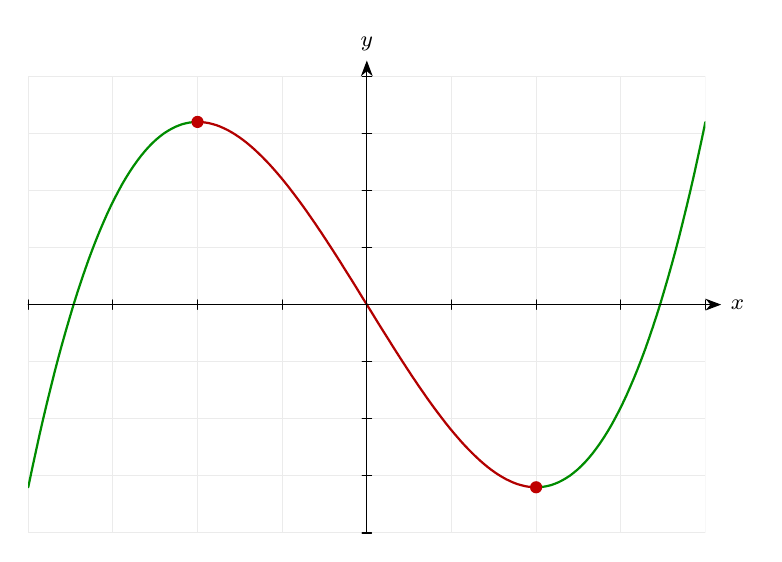
\begin{tikzpicture}[>={Stealth[length=2mm]},font=\footnotesize,line cap=round,line join=round]
\begin{scope}
\clip (0,0) rectangle (8.6,5.8);
\draw[gray!16] (0,0) grid[xstep=1.075,ystep=0.725] (8.6,5.8);
\draw[green!55!black,thick] (0,0.58) -- (0.048,0.809) -- (0.096,1.03) -- (0.143,1.245) -- (0.191,1.454) -- (0.239,1.656) -- (0.287,1.851) -- (0.334,2.04) -- (0.382,2.223) -- (0.43,2.399) -- (0.478,2.569) -- (0.526,2.733) -- (0.573,2.891) -- (0.621,3.043) -- (0.669,3.189) -- (0.717,3.33) -- (0.764,3.464) -- (0.812,3.593) -- (0.86,3.717) -- (0.908,3.835) -- (0.956,3.947) -- (1.003,4.054) -- (1.051,4.156) -- (1.099,4.253) -- (1.147,4.344) -- (1.194,4.431) -- (1.242,4.512) -- (1.29,4.589) -- (1.338,4.661) -- (1.386,4.728) -- (1.433,4.79) -- (1.481,4.848) -- (1.529,4.902) -- (1.577,4.951) -- (1.624,4.995) -- (1.672,5.035) -- (1.72,5.072) -- (1.768,5.103) -- (1.816,5.131) -- (1.863,5.155) -- (1.911,5.175) -- (1.959,5.192) -- (2.007,5.204) -- (2.054,5.213) -- (2.102,5.218) -- (2.15,5.22);
\draw[red!70!black,thick] (2.15,5.22) -- (2.198,5.218) -- (2.246,5.213) -- (2.293,5.205) -- (2.341,5.193) -- (2.389,5.179) -- (2.437,5.161) -- (2.484,5.14) -- (2.532,5.117) -- (2.58,5.09) -- (2.628,5.061) -- (2.676,5.029) -- (2.723,4.995) -- (2.771,4.958) -- (2.819,4.918) -- (2.867,4.876) -- (2.914,4.832) -- (2.962,4.786) -- (3.01,4.737) -- (3.058,4.687) -- (3.106,4.634) -- (3.153,4.58) -- (3.201,4.524) -- (3.249,4.466) -- (3.297,4.406) -- (3.344,4.345) -- (3.392,4.282) -- (3.44,4.218) -- (3.488,4.152) -- (3.536,4.085) -- (3.583,4.017) -- (3.631,3.948) -- (3.679,3.877) -- (3.727,3.806) -- (3.774,3.734) -- (3.822,3.661) -- (3.87,3.587) -- (3.918,3.512) -- (3.966,3.437) -- (4.013,3.361) -- (4.061,3.285) -- (4.109,3.209) -- (4.157,3.132) -- (4.204,3.055) -- (4.252,2.977) -- (4.3,2.9) -- (4.348,2.823) -- (4.396,2.745) -- (4.443,2.668) -- (4.491,2.591) -- (4.539,2.515) -- (4.587,2.439) -- (4.634,2.363) -- (4.682,2.288) -- (4.73,2.213) -- (4.778,2.139) -- (4.826,2.066) -- (4.873,1.994) -- (4.921,1.923) -- (4.969,1.852) -- (5.017,1.783) -- (5.064,1.715) -- (5.112,1.648) -- (5.16,1.582) -- (5.208,1.518) -- (5.256,1.455) -- (5.303,1.394) -- (5.351,1.334) -- (5.399,1.276) -- (5.447,1.22) -- (5.494,1.166) -- (5.542,1.113) -- (5.59,1.063) -- (5.638,1.014) -- (5.686,0.968) -- (5.733,0.924) -- (5.781,0.882) -- (5.829,0.842) -- (5.877,0.805) -- (5.924,0.771) -- (5.972,0.739) -- (6.02,0.71) -- (6.068,0.683) -- (6.116,0.66) -- (6.163,0.639) -- (6.211,0.621) -- (6.259,0.607) -- (6.307,0.595) -- (6.354,0.587) -- (6.402,0.582) -- (6.45,0.58);
\draw[green!55!black,thick] (6.45,0.58) -- (6.498,0.582) -- (6.546,0.587) -- (6.593,0.596) -- (6.641,0.608) -- (6.689,0.625) -- (6.737,0.645) -- (6.784,0.669) -- (6.832,0.697) -- (6.88,0.728) -- (6.928,0.765) -- (6.976,0.805) -- (7.023,0.849) -- (7.071,0.898) -- (7.119,0.952) -- (7.167,1.01) -- (7.214,1.072) -- (7.262,1.139) -- (7.31,1.211) -- (7.358,1.288) -- (7.406,1.369) -- (7.453,1.456) -- (7.501,1.547) -- (7.549,1.644) -- (7.597,1.746) -- (7.644,1.853) -- (7.692,1.965) -- (7.74,2.083) -- (7.788,2.207) -- (7.836,2.336) -- (7.883,2.47) -- (7.931,2.611) -- (7.979,2.757) -- (8.027,2.909) -- (8.074,3.067) -- (8.122,3.231) -- (8.17,3.401) -- (8.218,3.577) -- (8.266,3.76) -- (8.313,3.949) -- (8.361,4.144) -- (8.409,4.346) -- (8.457,4.555) -- (8.504,4.77) -- (8.552,4.991) -- (8.6,5.22);
\end{scope}
\draw[->] (0,2.9) -- (8.8,2.9) node[right]{$x$};
\draw[->] (4.3,0) -- (4.3,6) node[above]{$y$};
\draw (0,2.84) -- (0,2.96);
\draw (1.075,2.84) -- (1.075,2.96);
\draw (2.15,2.84) -- (2.15,2.96);
\draw (3.225,2.84) -- (3.225,2.96);
\draw (5.375,2.84) -- (5.375,2.96);
\draw (6.45,2.84) -- (6.45,2.96);
\draw (7.525,2.84) -- (7.525,2.96);
\draw (8.6,2.84) -- (8.6,2.96);
\draw (4.24,0) -- (4.36,0);
\draw (4.24,0.725) -- (4.36,0.725);
\draw (4.24,1.45) -- (4.36,1.45);
\draw (4.24,2.175) -- (4.36,2.175);
\draw (4.24,3.625) -- (4.36,3.625);
\draw (4.24,4.35) -- (4.36,4.35);
\draw (4.24,5.075) -- (4.36,5.075);
\draw (4.24,5.8) -- (4.36,5.8);
\fill[red!75!black] (2.15,5.22) circle (2.2pt);
\fill[red!75!black] (6.45,0.58) circle (2.2pt);
\end{tikzpicture}
}
\end{center}
\small Curve coloured green where increasing, red where decreasing.\normalsize

\medskip\hrule

\section*{Derivatives and Graphs 45\quad\small\texttt{(d4-045)}}
\addcontentsline{toc}{section}{Derivatives and Graphs 45 (d4-045)}
\textit{Difficulty: Standard \quad\textbar\quad Marks: 4}

\question{Find the values of \( x \) for which the curve \( y = x^4 - 4x^3 \) is increasing.}

\textbf{Worked solution.}

\textit{Step 1: Differentiate.}
\[\begin{gathered}
\frac{\mathrm{d}y}{\mathrm{d}x} = 4x^3 - 12x^2 = 4x^2(x - 3)
\end{gathered}\]
Factor out \( 4x^2 \).

\textit{Step 2: Sign analysis.}
\[\begin{gathered}
4x^2 \geq 0 \Rightarrow \text{sign depends on } (x - 3)
\end{gathered}\]
\( 4x^2 = 0 \) at \( x = 0 \) (boundary only).

\textit{Step 3: \( \frac{\mathrm{d}y}{\mathrm{d}x} > 0 \) when \( x - 3 > 0 \).}
\[\begin{gathered}
x > 3
\end{gathered}\]
For \( x = 0 \) the derivative is zero; elsewhere negative for \( x < 3, x \ne 0 \).

\begin{answerbox}
\textbf{Final answer:}\quad Increasing for \(\displaystyle  x > 3 \).
\end{answerbox}
\textbf{Diagram.}

\begin{center}
\resizebox{\ifdim\width>\linewidth \linewidth\else \width\fi}{!}{%
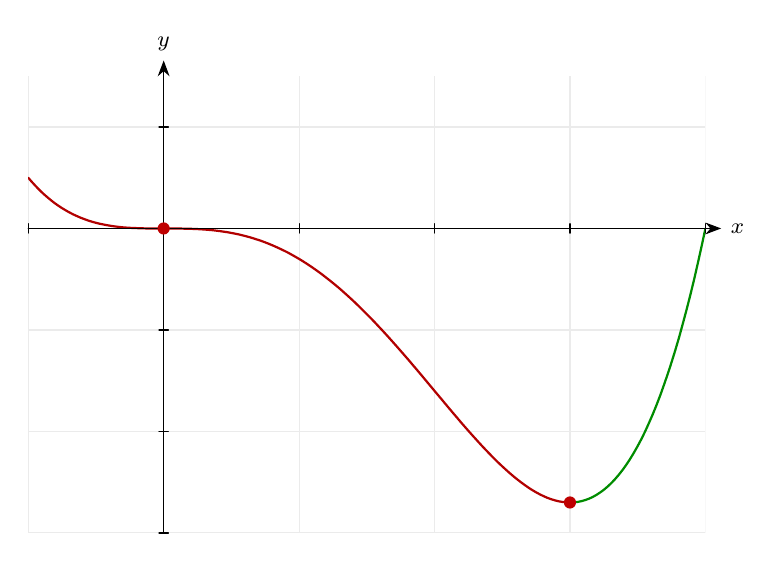
\begin{tikzpicture}[>={Stealth[length=2mm]},font=\footnotesize,line cap=round,line join=round]
\begin{scope}
\clip (0,0) rectangle (8.6,5.8);
\draw[gray!16] (0,0) grid[xstep=1.72,ystep=1.289] (8.6,5.8);
\draw[red!70!black,thick] (0,4.511) -- (0.048,4.456) -- (0.096,4.404) -- (0.143,4.355) -- (0.191,4.309) -- (0.239,4.267) -- (0.287,4.227) -- (0.334,4.19) -- (0.382,4.156) -- (0.43,4.125) -- (0.478,4.096) -- (0.526,4.069) -- (0.573,4.045) -- (0.621,4.023) -- (0.669,4.002) -- (0.717,3.984) -- (0.764,3.967) -- (0.812,3.952) -- (0.86,3.939) -- (0.908,3.927) -- (0.956,3.917) -- (1.003,3.908) -- (1.051,3.9) -- (1.099,3.893) -- (1.147,3.887) -- (1.194,3.882) -- (1.242,3.878) -- (1.29,3.875) -- (1.338,3.873) -- (1.386,3.871) -- (1.433,3.869) -- (1.481,3.868) -- (1.529,3.867) -- (1.577,3.867) -- (1.624,3.867) -- (1.672,3.867) -- (1.72,3.867);
\draw[red!70!black,thick] (1.72,3.867) -- (1.768,3.867) -- (1.816,3.867) -- (1.863,3.866) -- (1.911,3.866) -- (1.959,3.865) -- (2.007,3.864) -- (2.054,3.863) -- (2.102,3.861) -- (2.15,3.859) -- (2.198,3.856) -- (2.246,3.853) -- (2.293,3.849) -- (2.341,3.845) -- (2.389,3.839) -- (2.437,3.833) -- (2.484,3.826) -- (2.532,3.819) -- (2.58,3.81) -- (2.628,3.801) -- (2.676,3.791) -- (2.723,3.779) -- (2.771,3.767) -- (2.819,3.754) -- (2.867,3.739) -- (2.914,3.724) -- (2.962,3.708) -- (3.01,3.69) -- (3.058,3.671) -- (3.106,3.651) -- (3.153,3.63) -- (3.201,3.608) -- (3.249,3.585) -- (3.297,3.561) -- (3.344,3.535) -- (3.392,3.508) -- (3.44,3.48) -- (3.488,3.451) -- (3.536,3.42) -- (3.583,3.389) -- (3.631,3.356) -- (3.679,3.322) -- (3.727,3.287) -- (3.774,3.25) -- (3.822,3.213) -- (3.87,3.174) -- (3.918,3.135) -- (3.966,3.094) -- (4.013,3.052) -- (4.061,3.009) -- (4.109,2.965) -- (4.157,2.92) -- (4.204,2.874) -- (4.252,2.827) -- (4.3,2.779) -- (4.348,2.73) -- (4.396,2.681) -- (4.443,2.63) -- (4.491,2.579) -- (4.539,2.527) -- (4.587,2.474) -- (4.634,2.421) -- (4.682,2.367) -- (4.73,2.312) -- (4.778,2.257) -- (4.826,2.202) -- (4.873,2.146) -- (4.921,2.09) -- (4.969,2.033) -- (5.017,1.976) -- (5.064,1.919) -- (5.112,1.862) -- (5.16,1.804) -- (5.208,1.747) -- (5.256,1.69) -- (5.303,1.633) -- (5.351,1.576) -- (5.399,1.519) -- (5.447,1.463) -- (5.494,1.407) -- (5.542,1.352) -- (5.59,1.297) -- (5.638,1.243) -- (5.686,1.19) -- (5.733,1.138) -- (5.781,1.086) -- (5.829,1.036) -- (5.877,0.986) -- (5.924,0.938) -- (5.972,0.891) -- (6.02,0.846) -- (6.068,0.802) -- (6.116,0.759) -- (6.163,0.719) -- (6.211,0.68) -- (6.259,0.643) -- (6.307,0.608) -- (6.354,0.575) -- (6.402,0.544) -- (6.45,0.516) -- (6.498,0.49) -- (6.546,0.467) -- (6.593,0.446) -- (6.641,0.429) -- (6.689,0.414) -- (6.737,0.402) -- (6.784,0.394) -- (6.832,0.388) -- (6.88,0.387);
\draw[green!55!black,thick] (6.88,0.387) -- (6.928,0.388) -- (6.976,0.394) -- (7.023,0.403) -- (7.071,0.417) -- (7.119,0.434) -- (7.167,0.456) -- (7.214,0.482) -- (7.262,0.513) -- (7.31,0.548) -- (7.358,0.589) -- (7.406,0.634) -- (7.453,0.684) -- (7.501,0.74) -- (7.549,0.801) -- (7.597,0.868) -- (7.644,0.94) -- (7.692,1.019) -- (7.74,1.104) -- (7.788,1.194) -- (7.836,1.292) -- (7.883,1.396) -- (7.931,1.506) -- (7.979,1.624) -- (8.027,1.749) -- (8.074,1.881) -- (8.122,2.02) -- (8.17,2.167) -- (8.218,2.322) -- (8.266,2.485) -- (8.313,2.657) -- (8.361,2.836) -- (8.409,3.024) -- (8.457,3.221) -- (8.504,3.427) -- (8.552,3.642) -- (8.6,3.867);
\end{scope}
\draw[->] (0,3.867) -- (8.8,3.867) node[right]{$x$};
\draw[->] (1.72,0) -- (1.72,6) node[above]{$y$};
\draw (0,3.807) -- (0,3.927);
\draw (3.44,3.807) -- (3.44,3.927);
\draw (5.16,3.807) -- (5.16,3.927);
\draw (6.88,3.807) -- (6.88,3.927);
\draw (8.6,3.807) -- (8.6,3.927);
\draw (1.66,0) -- (1.78,0);
\draw (1.66,1.289) -- (1.78,1.289);
\draw (1.66,2.578) -- (1.78,2.578);
\draw (1.66,5.156) -- (1.78,5.156);
\fill[red!75!black] (1.72,3.867) circle (2.2pt);
\fill[red!75!black] (6.88,0.387) circle (2.2pt);
\end{tikzpicture}
}
\end{center}
\small Curve coloured green where increasing, red where decreasing.\normalsize

\medskip\hrule

\section*{Derivatives and Graphs 46\quad\small\texttt{(d4-046)}}
\addcontentsline{toc}{section}{Derivatives and Graphs 46 (d4-046)}
\textit{Difficulty: Standard \quad\textbar\quad Marks: 5}

\question{For \( f(x) = x + \dfrac{4}{x} \), \( x > 0 \), find the range of values of \( x \) for which \( f \) is increasing.}

\textbf{Worked solution.}

\textit{Step 1: Rewrite and differentiate.}
\[\begin{gathered}
f(x) = x + 4x^{-1} \Rightarrow f'(x) = 1 - 4x^{-2} = 1 - \dfrac{4}{x^2}
\end{gathered}\]
Apply the power rule.

\textit{Step 2: Solve \( f'(x) > 0 \).}
\[\begin{gathered}
1 > \dfrac{4}{x^2} \Rightarrow x^2 > 4 \Rightarrow x > 2 \text{ (since } x > 0\text{)}
\end{gathered}\]
Rearrange carefully.

\begin{answerbox}
\textbf{Final answer:}\quad \(\displaystyle  f \) is increasing on \(\displaystyle  x > 2 \).
\end{answerbox}
\textbf{Diagram.}

\begin{center}
\resizebox{\ifdim\width>\linewidth \linewidth\else \width\fi}{!}{%
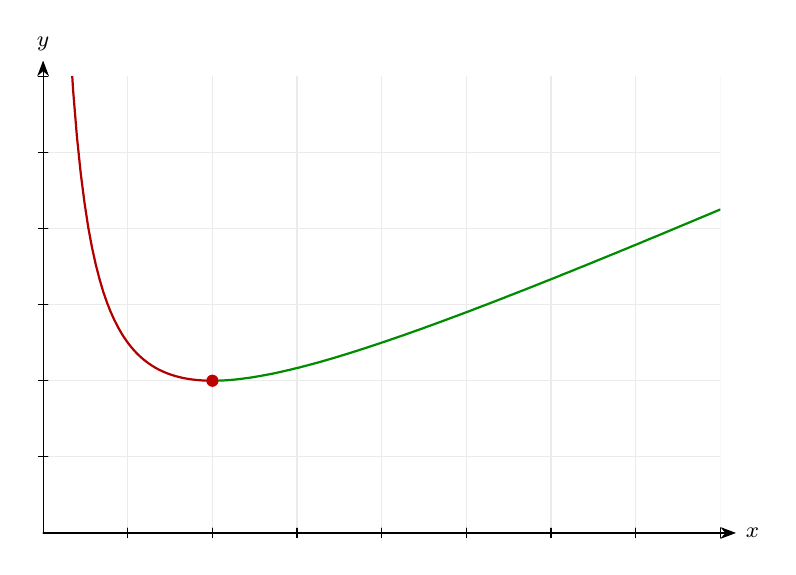
\begin{tikzpicture}[>={Stealth[length=2mm]},font=\footnotesize,line cap=round,line join=round]
\begin{scope}
\clip (0,0) rectangle (8.6,5.8);
\draw[gray!16] (0,0) grid[xstep=1.075,ystep=0.967] (8.6,5.8);
\draw[red!70!black,thick] (0.048,11.6) -- (0.096,11.6) -- (0.143,11.6) -- (0.191,10.961) -- (0.239,8.807) -- (0.287,7.379) -- (0.334,6.365) -- (0.382,5.609) -- (0.43,5.027) -- (0.478,4.565) -- (0.526,4.191) -- (0.573,3.883) -- (0.621,3.625) -- (0.669,3.408) -- (0.717,3.222) -- (0.764,3.062) -- (0.812,2.924) -- (0.86,2.803) -- (0.908,2.698) -- (0.956,2.605) -- (1.003,2.523) -- (1.051,2.45) -- (1.099,2.385) -- (1.147,2.328) -- (1.194,2.277) -- (1.242,2.232) -- (1.29,2.191) -- (1.338,2.155) -- (1.386,2.123) -- (1.433,2.094) -- (1.481,2.069) -- (1.529,2.047) -- (1.577,2.027) -- (1.624,2.01) -- (1.672,1.995) -- (1.72,1.982) -- (1.768,1.97) -- (1.816,1.961) -- (1.863,1.953) -- (1.911,1.947) -- (1.959,1.942) -- (2.007,1.938) -- (2.054,1.935) -- (2.102,1.934) -- (2.15,1.933);
\draw[green!55!black,thick] (2.15,1.933) -- (2.198,1.934) -- (2.246,1.935) -- (2.293,1.937) -- (2.341,1.94) -- (2.389,1.944) -- (2.437,1.948) -- (2.484,1.954) -- (2.532,1.959) -- (2.58,1.966) -- (2.628,1.972) -- (2.676,1.98) -- (2.723,1.988) -- (2.771,1.996) -- (2.819,2.005) -- (2.867,2.014) -- (2.914,2.023) -- (2.962,2.033) -- (3.01,2.044) -- (3.058,2.055) -- (3.106,2.066) -- (3.153,2.077) -- (3.201,2.089) -- (3.249,2.1) -- (3.297,2.113) -- (3.344,2.125) -- (3.392,2.138) -- (3.44,2.151) -- (3.488,2.164) -- (3.536,2.177) -- (3.583,2.191) -- (3.631,2.205) -- (3.679,2.219) -- (3.727,2.233) -- (3.774,2.248) -- (3.822,2.262) -- (3.87,2.277) -- (3.918,2.292) -- (3.966,2.307) -- (4.013,2.322) -- (4.061,2.338) -- (4.109,2.353) -- (4.157,2.369) -- (4.204,2.385) -- (4.252,2.401) -- (4.3,2.417) -- (4.348,2.433) -- (4.396,2.449) -- (4.443,2.466) -- (4.491,2.482) -- (4.539,2.499) -- (4.587,2.515) -- (4.634,2.532) -- (4.682,2.549) -- (4.73,2.566) -- (4.778,2.583) -- (4.826,2.6) -- (4.873,2.618) -- (4.921,2.635) -- (4.969,2.652) -- (5.017,2.67) -- (5.064,2.687) -- (5.112,2.705) -- (5.16,2.723) -- (5.208,2.741) -- (5.256,2.758) -- (5.303,2.776) -- (5.351,2.794) -- (5.399,2.812) -- (5.447,2.83) -- (5.494,2.849) -- (5.542,2.867) -- (5.59,2.885) -- (5.638,2.903) -- (5.686,2.922) -- (5.733,2.94) -- (5.781,2.959) -- (5.829,2.977) -- (5.877,2.996) -- (5.924,3.015) -- (5.972,3.033) -- (6.02,3.052) -- (6.068,3.071) -- (6.116,3.089) -- (6.163,3.108) -- (6.211,3.127) -- (6.259,3.146) -- (6.307,3.165) -- (6.354,3.184) -- (6.402,3.203) -- (6.45,3.222) -- (6.498,3.241) -- (6.546,3.26) -- (6.593,3.28) -- (6.641,3.299) -- (6.689,3.318) -- (6.737,3.337) -- (6.784,3.357) -- (6.832,3.376) -- (6.88,3.395) -- (6.928,3.415) -- (6.976,3.434) -- (7.023,3.454) -- (7.071,3.473) -- (7.119,3.493) -- (7.167,3.512) -- (7.214,3.532) -- (7.262,3.551) -- (7.31,3.571) -- (7.358,3.591) -- (7.406,3.61) -- (7.453,3.63) -- (7.501,3.65) -- (7.549,3.669) -- (7.597,3.689) -- (7.644,3.709) -- (7.692,3.729) -- (7.74,3.749) -- (7.788,3.768) -- (7.836,3.788) -- (7.883,3.808) -- (7.931,3.828) -- (7.979,3.848) -- (8.027,3.868) -- (8.074,3.888) -- (8.122,3.908) -- (8.17,3.928) -- (8.218,3.948) -- (8.266,3.968) -- (8.313,3.988) -- (8.361,4.008) -- (8.409,4.028) -- (8.457,4.048) -- (8.504,4.068) -- (8.552,4.088) -- (8.6,4.108);
\end{scope}
\draw[->] (0,0) -- (8.8,0) node[right]{$x$};
\draw[->] (0,0) -- (0,6) node[above]{$y$};
\draw (1.075,-0.06) -- (1.075,0.06);
\draw (2.15,-0.06) -- (2.15,0.06);
\draw (3.225,-0.06) -- (3.225,0.06);
\draw (4.3,-0.06) -- (4.3,0.06);
\draw (5.375,-0.06) -- (5.375,0.06);
\draw (6.45,-0.06) -- (6.45,0.06);
\draw (7.525,-0.06) -- (7.525,0.06);
\draw (8.6,-0.06) -- (8.6,0.06);
\draw (-0.06,0.967) -- (0.06,0.967);
\draw (-0.06,1.933) -- (0.06,1.933);
\draw (-0.06,2.9) -- (0.06,2.9);
\draw (-0.06,3.867) -- (0.06,3.867);
\draw (-0.06,4.833) -- (0.06,4.833);
\draw (-0.06,5.8) -- (0.06,5.8);
\fill[red!75!black] (2.15,1.933) circle (2.2pt);
\end{tikzpicture}
}
\end{center}
\small Curve coloured green where increasing, red where decreasing.\normalsize

\medskip\hrule

\section*{Derivatives and Graphs 47\quad\small\texttt{(d4-047)}}
\addcontentsline{toc}{section}{Derivatives and Graphs 47 (d4-047)}
\textit{Difficulty: Standard \quad\textbar\quad Marks: 5}

\question{Show that \( f(x) = \dfrac{x^3}{3} - 2x^2 + 5x + 1 \) is an increasing function for all real \( x \).}

\textbf{Worked solution.}

\textit{Step 1: Differentiate.}
\[\begin{gathered}
f'(x) = x^2 - 4x + 5
\end{gathered}\]
Apply the power rule.

\textit{Step 2: Complete the square.}
\[\begin{gathered}
f'(x) = (x - 2)^2 + 1
\end{gathered}\]
Rewrite to show the minimum value.

\textit{Step 3: Minimum value.}
\[\begin{gathered}
f'(x) \geq 1 > 0 \text{ for all } x
\end{gathered}\]
Since a square is non-negative, the minimum is 1.

\begin{answerbox}
\textbf{Final answer:}\quad \(\displaystyle  f'(x) \geq 1 > 0 \) for all \(\displaystyle  x \), so \(\displaystyle  f \) is always increasing.
\end{answerbox}
\textbf{Diagram.}

\begin{center}
\resizebox{\ifdim\width>\linewidth \linewidth\else \width\fi}{!}{%
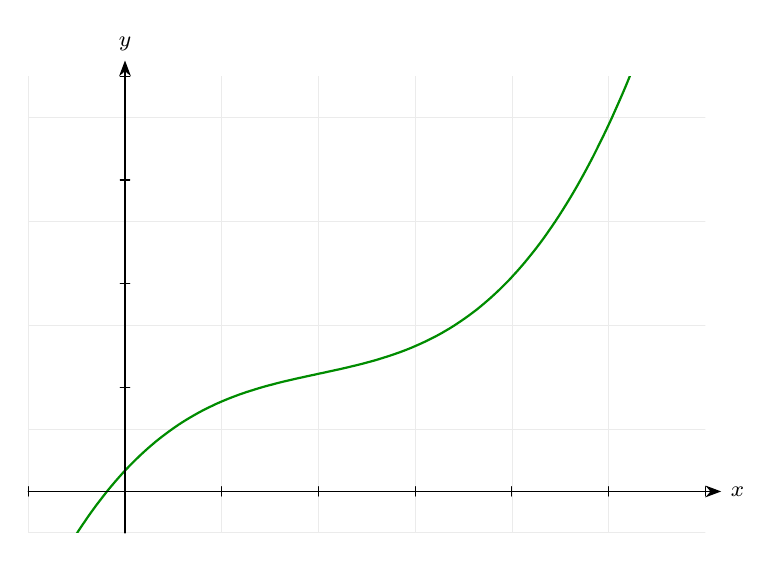
\begin{tikzpicture}[>={Stealth[length=2mm]},font=\footnotesize,line cap=round,line join=round]
\begin{scope}
\clip (0,0) rectangle (8.6,5.8);
\draw[gray!16] (0,-0.791) grid[xstep=1.229,ystep=1.318] (8.6,5.8);
\draw[green!55!black,thick] (0,-1.142) -- (0.048,-1.041) -- (0.096,-0.942) -- (0.143,-0.845) -- (0.191,-0.751) -- (0.239,-0.659) -- (0.287,-0.569) -- (0.334,-0.482) -- (0.382,-0.396) -- (0.43,-0.313) -- (0.478,-0.232) -- (0.526,-0.152) -- (0.573,-0.075) -- (0.621,0) -- (0.669,0.073) -- (0.717,0.144) -- (0.764,0.213) -- (0.812,0.28) -- (0.86,0.346) -- (0.908,0.409) -- (0.956,0.471) -- (1.003,0.531) -- (1.051,0.589) -- (1.099,0.646) -- (1.147,0.701) -- (1.194,0.754) -- (1.242,0.805) -- (1.29,0.856) -- (1.338,0.904) -- (1.386,0.951) -- (1.433,0.996) -- (1.481,1.04) -- (1.529,1.083) -- (1.577,1.124) -- (1.624,1.164) -- (1.672,1.202) -- (1.72,1.239) -- (1.768,1.275) -- (1.816,1.31) -- (1.863,1.343) -- (1.911,1.376) -- (1.959,1.407) -- (2.007,1.437) -- (2.054,1.465) -- (2.102,1.493) -- (2.15,1.52) -- (2.198,1.546) -- (2.246,1.571) -- (2.293,1.594) -- (2.341,1.617) -- (2.389,1.64) -- (2.437,1.661) -- (2.484,1.681) -- (2.532,1.701) -- (2.58,1.72) -- (2.628,1.738) -- (2.676,1.756) -- (2.723,1.772) -- (2.771,1.789) -- (2.819,1.804) -- (2.867,1.819) -- (2.914,1.834) -- (2.962,1.848) -- (3.01,1.862) -- (3.058,1.875) -- (3.106,1.887) -- (3.153,1.9) -- (3.201,1.912) -- (3.249,1.924) -- (3.297,1.935) -- (3.344,1.946) -- (3.392,1.957) -- (3.44,1.968) -- (3.488,1.978) -- (3.536,1.989) -- (3.583,1.999) -- (3.631,2.009) -- (3.679,2.02) -- (3.727,2.03) -- (3.774,2.04) -- (3.822,2.051) -- (3.87,2.061) -- (3.918,2.072) -- (3.966,2.082) -- (4.013,2.093) -- (4.061,2.104) -- (4.109,2.116) -- (4.157,2.127) -- (4.204,2.139) -- (4.252,2.151) -- (4.3,2.164) -- (4.348,2.177) -- (4.396,2.19) -- (4.443,2.204) -- (4.491,2.219) -- (4.539,2.234) -- (4.587,2.249) -- (4.634,2.265) -- (4.682,2.282) -- (4.73,2.299) -- (4.778,2.317) -- (4.826,2.336) -- (4.873,2.355) -- (4.921,2.376) -- (4.969,2.397) -- (5.017,2.419) -- (5.064,2.441) -- (5.112,2.465) -- (5.16,2.489) -- (5.208,2.515) -- (5.256,2.541) -- (5.303,2.569) -- (5.351,2.597) -- (5.399,2.627) -- (5.447,2.658) -- (5.494,2.69) -- (5.542,2.723) -- (5.59,2.757) -- (5.638,2.793) -- (5.686,2.829) -- (5.733,2.867) -- (5.781,2.907) -- (5.829,2.948) -- (5.877,2.99) -- (5.924,3.033) -- (5.972,3.078) -- (6.02,3.125) -- (6.068,3.173) -- (6.116,3.222) -- (6.163,3.274) -- (6.211,3.326) -- (6.259,3.381) -- (6.307,3.437) -- (6.354,3.495) -- (6.402,3.554) -- (6.45,3.615) -- (6.498,3.678) -- (6.546,3.743) -- (6.593,3.81) -- (6.641,3.879) -- (6.689,3.949) -- (6.737,4.022) -- (6.784,4.096) -- (6.832,4.173) -- (6.88,4.251) -- (6.928,4.332) -- (6.976,4.415) -- (7.023,4.499) -- (7.071,4.586) -- (7.119,4.676) -- (7.167,4.767) -- (7.214,4.861) -- (7.262,4.957) -- (7.31,5.055) -- (7.358,5.156) -- (7.406,5.259) -- (7.453,5.364) -- (7.501,5.472) -- (7.549,5.582) -- (7.597,5.695) -- (7.644,5.811) -- (7.692,5.929) -- (7.74,6.049) -- (7.788,6.173) -- (7.836,6.298) -- (7.883,6.427) -- (7.931,6.558) -- (7.979,6.692) -- (8.027,6.829) -- (8.074,6.969) -- (8.122,7.111) -- (8.17,7.257) -- (8.218,7.405) -- (8.266,7.556) -- (8.313,7.711) -- (8.361,7.868) -- (8.409,8.028) -- (8.457,8.191) -- (8.504,8.358) -- (8.552,8.527) -- (8.6,8.7);
\end{scope}
\draw[->] (0,0.527) -- (8.8,0.527) node[right]{$x$};
\draw[->] (1.229,0) -- (1.229,6) node[above]{$y$};
\draw (0,0.467) -- (0,0.587);
\draw (2.457,0.467) -- (2.457,0.587);
\draw (3.686,0.467) -- (3.686,0.587);
\draw (4.914,0.467) -- (4.914,0.587);
\draw (6.143,0.467) -- (6.143,0.587);
\draw (7.371,0.467) -- (7.371,0.587);
\draw (8.6,0.467) -- (8.6,0.587);
\draw (1.169,1.845) -- (1.289,1.845);
\draw (1.169,3.164) -- (1.289,3.164);
\draw (1.169,4.482) -- (1.289,4.482);
\draw (1.169,5.8) -- (1.289,5.8);
\end{tikzpicture}
}
\end{center}
\small Curve coloured green where increasing, red where decreasing.\normalsize

\medskip\hrule

\section*{Derivatives and Graphs 48\quad\small\texttt{(d4-048)}}
\addcontentsline{toc}{section}{Derivatives and Graphs 48 (d4-048)}
\textit{Difficulty: Standard \quad\textbar\quad Marks: 5}

\question{The function \( y = x^3 - 3x^2 - 24x \) is increasing for \( x < a \) and \( x > b \), where \( a < b \). Find \( a \) and \( b \).}

\textbf{Worked solution.}

\textit{Step 1: Differentiate.}
\[\begin{gathered}
\frac{\mathrm{d}y}{\mathrm{d}x} = 3x^2 - 6x - 24
\end{gathered}\]
Apply the power rule.

\textit{Step 2: Factorise.}
\[\begin{gathered}
3(x^2 - 2x - 8) = 3(x - 4)(x + 2)
\end{gathered}\]
Factor out 3 and factorise the quadratic.

\textit{Step 3: \( y' > 0 \) outside the roots.}
\[\begin{gathered}
x < -2 \text{ or } x > 4
\end{gathered}\]
Quadratic opens upwards.

\begin{answerbox}
\textbf{Final answer:}\quad \(\displaystyle  a = -2 \) and \(\displaystyle  b = 4 \).
\end{answerbox}
\textbf{Diagram.}

\begin{center}
\resizebox{\ifdim\width>\linewidth \linewidth\else \width\fi}{!}{%
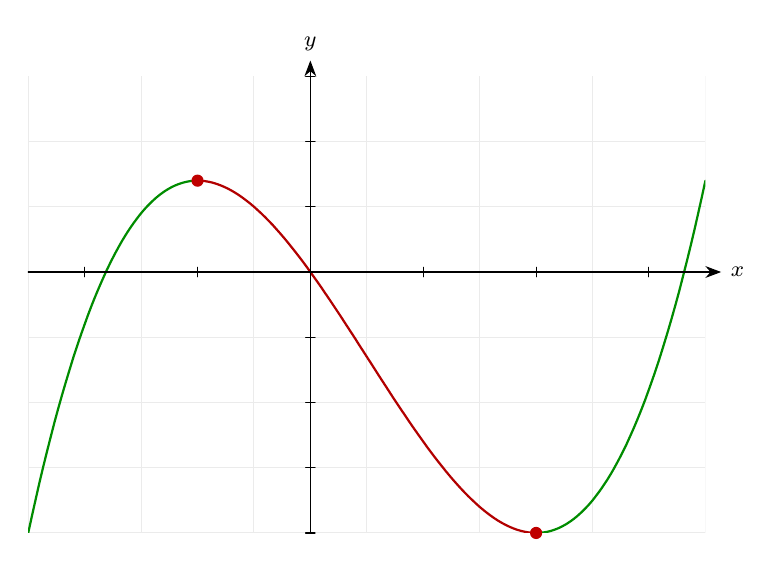
\begin{tikzpicture}[>={Stealth[length=2mm]},font=\footnotesize,line cap=round,line join=round]
\begin{scope}
\clip (0,0) rectangle (8.6,5.8);
\draw[gray!16] (-0.717,0) grid[xstep=1.433,ystep=0.829] (8.6,5.8);
\draw[green!55!black,thick] (0,0) -- (0.048,0.22) -- (0.096,0.434) -- (0.143,0.642) -- (0.191,0.843) -- (0.239,1.037) -- (0.287,1.226) -- (0.334,1.408) -- (0.382,1.584) -- (0.43,1.754) -- (0.478,1.918) -- (0.526,2.076) -- (0.573,2.229) -- (0.621,2.375) -- (0.669,2.516) -- (0.717,2.651) -- (0.764,2.781) -- (0.812,2.906) -- (0.86,3.025) -- (0.908,3.138) -- (0.956,3.247) -- (1.003,3.35) -- (1.051,3.448) -- (1.099,3.542) -- (1.147,3.63) -- (1.194,3.713) -- (1.242,3.792) -- (1.29,3.866) -- (1.338,3.935) -- (1.386,4) -- (1.433,4.06) -- (1.481,4.116) -- (1.529,4.167) -- (1.577,4.214) -- (1.624,4.257) -- (1.672,4.296) -- (1.72,4.331) -- (1.768,4.362) -- (1.816,4.389) -- (1.863,4.412) -- (1.911,4.431) -- (1.959,4.447) -- (2.007,4.459) -- (2.054,4.468) -- (2.102,4.473) -- (2.15,4.474);
\draw[red!70!black,thick] (2.15,4.474) -- (2.198,4.473) -- (2.246,4.468) -- (2.293,4.46) -- (2.341,4.449) -- (2.389,4.434) -- (2.437,4.417) -- (2.484,4.397) -- (2.532,4.375) -- (2.58,4.349) -- (2.628,4.321) -- (2.676,4.29) -- (2.723,4.257) -- (2.771,4.221) -- (2.819,4.183) -- (2.867,4.143) -- (2.914,4.1) -- (2.962,4.056) -- (3.01,4.009) -- (3.058,3.96) -- (3.106,3.91) -- (3.153,3.857) -- (3.201,3.803) -- (3.249,3.747) -- (3.297,3.689) -- (3.344,3.63) -- (3.392,3.57) -- (3.44,3.508) -- (3.488,3.445) -- (3.536,3.38) -- (3.583,3.314) -- (3.631,3.247) -- (3.679,3.18) -- (3.727,3.111) -- (3.774,3.041) -- (3.822,2.971) -- (3.87,2.899) -- (3.918,2.827) -- (3.966,2.755) -- (4.013,2.682) -- (4.061,2.608) -- (4.109,2.535) -- (4.157,2.461) -- (4.204,2.386) -- (4.252,2.312) -- (4.3,2.237) -- (4.348,2.163) -- (4.396,2.088) -- (4.443,2.014) -- (4.491,1.94) -- (4.539,1.866) -- (4.587,1.792) -- (4.634,1.719) -- (4.682,1.647) -- (4.73,1.575) -- (4.778,1.504) -- (4.826,1.433) -- (4.873,1.363) -- (4.921,1.295) -- (4.969,1.227) -- (5.017,1.16) -- (5.064,1.094) -- (5.112,1.03) -- (5.16,0.966) -- (5.208,0.904) -- (5.256,0.844) -- (5.303,0.785) -- (5.351,0.727) -- (5.399,0.671) -- (5.447,0.617) -- (5.494,0.565) -- (5.542,0.514) -- (5.59,0.465) -- (5.638,0.419) -- (5.686,0.374) -- (5.733,0.331) -- (5.781,0.291) -- (5.829,0.253) -- (5.877,0.217) -- (5.924,0.184) -- (5.972,0.153) -- (6.02,0.125) -- (6.068,0.1) -- (6.116,0.077) -- (6.163,0.057) -- (6.211,0.04) -- (6.259,0.026) -- (6.307,0.015) -- (6.354,0.007) -- (6.402,0.002) -- (6.45,0);
\draw[green!55!black,thick] (6.45,0) -- (6.498,0.002) -- (6.546,0.007) -- (6.593,0.015) -- (6.641,0.027) -- (6.689,0.043) -- (6.737,0.062) -- (6.784,0.085) -- (6.832,0.112) -- (6.88,0.143) -- (6.928,0.178) -- (6.976,0.217) -- (7.023,0.26) -- (7.071,0.307) -- (7.119,0.358) -- (7.167,0.414) -- (7.214,0.475) -- (7.262,0.539) -- (7.31,0.609) -- (7.358,0.682) -- (7.406,0.761) -- (7.453,0.844) -- (7.501,0.933) -- (7.549,1.026) -- (7.597,1.124) -- (7.644,1.228) -- (7.692,1.336) -- (7.74,1.45) -- (7.788,1.569) -- (7.836,1.693) -- (7.883,1.823) -- (7.931,1.958) -- (7.979,2.099) -- (8.027,2.246) -- (8.074,2.398) -- (8.122,2.556) -- (8.17,2.72) -- (8.218,2.89) -- (8.266,3.066) -- (8.313,3.249) -- (8.361,3.437) -- (8.409,3.632) -- (8.457,3.833) -- (8.504,4.04) -- (8.552,4.254) -- (8.6,4.474);
\end{scope}
\draw[->] (0,3.314) -- (8.8,3.314) node[right]{$x$};
\draw[->] (3.583,0) -- (3.583,6) node[above]{$y$};
\draw (0.717,3.254) -- (0.717,3.374);
\draw (2.15,3.254) -- (2.15,3.374);
\draw (5.017,3.254) -- (5.017,3.374);
\draw (6.45,3.254) -- (6.45,3.374);
\draw (7.883,3.254) -- (7.883,3.374);
\draw (3.523,0) -- (3.643,0);
\draw (3.523,0.829) -- (3.643,0.829);
\draw (3.523,1.657) -- (3.643,1.657);
\draw (3.523,2.486) -- (3.643,2.486);
\draw (3.523,4.143) -- (3.643,4.143);
\draw (3.523,4.971) -- (3.643,4.971);
\draw (3.523,5.8) -- (3.643,5.8);
\fill[red!75!black] (2.15,4.474) circle (2.2pt);
\fill[red!75!black] (6.45,0) circle (2.2pt);
\end{tikzpicture}
}
\end{center}
\small Curve coloured green where increasing, red where decreasing.\normalsize

\medskip\hrule

\section*{Derivatives and Graphs 49\quad\small\texttt{(d4-049)}}
\addcontentsline{toc}{section}{Derivatives and Graphs 49 (d4-049)}
\textit{Difficulty: Standard \quad\textbar\quad Marks: 8}

\question{For the curve \( y = x^3 - 6x^2 + 9x \): (a) find the axis intercepts, (b) find the coordinates of the stationary points and classify each, (c) describe the shape of the curve.}

\textbf{Worked solution.}

\textit{Step 1: (a) \( x \)-intercepts: set \( y = 0 \).}
\[\begin{gathered}
x(x^2 - 6x + 9) = 0 \Rightarrow x(x - 3)^2 = 0
\end{gathered}\]
Factor out \( x \), then a perfect square.

\textit{Step 2: Intercepts.}
\[\begin{gathered}
x = 0 \text{ or } x = 3; \; y\text{-intercept} = 0
\end{gathered}\]
Curve crosses at origin and touches at \( (3, 0) \).

\textit{Step 3: (b) Differentiate.}
\[\begin{gathered}
\frac{\mathrm{d}y}{\mathrm{d}x} = 3x^2 - 12x + 9 = 3(x - 1)(x - 3)
\end{gathered}\]
Factorise.

\textit{Step 4: Stationary points.}
\[\begin{gathered}
x = 1: \; y = 1 - 6 + 9 = 4 \\ x = 3: \; y = 27 - 54 + 27 = 0
\end{gathered}\]
Substitute.

\textit{Step 5: Classify with second derivative.}
\[\begin{gathered}
y'' = 6x - 12 \\ y''(1) = -6 < 0\; (\text{max}) \\ y''(3) = 6 > 0\; (\text{min})
\end{gathered}\]
Second derivative test.

\begin{answerbox}
\textbf{Final answer:}\quad (a) Through origin; touches \(\displaystyle  x \)-axis at \(\displaystyle  (3, 0) \). \\[3pt]  (b) Maximum at \(\displaystyle  (1, 4) \), minimum at \(\displaystyle  (3, 0) \). \\[3pt]  (c) Cubic starting from \(\displaystyle  -\infty \), rising to a max at \(\displaystyle  (1, 4) \), falling to touch the \(\displaystyle  x \)-axis at \(\displaystyle  (3, 0) \), then rising to \(\displaystyle  +\infty \).
\end{answerbox}
\textbf{Diagram.}

\begin{center}
\resizebox{\ifdim\width>\linewidth \linewidth\else \width\fi}{!}{%
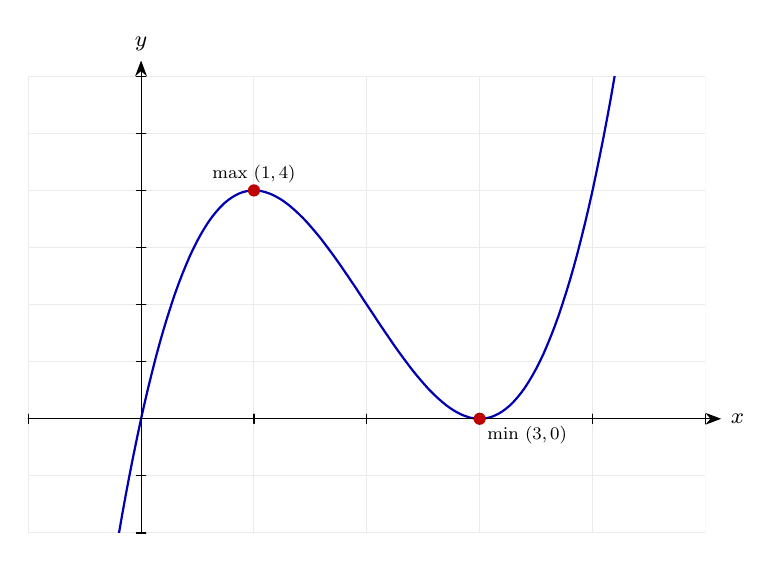
\begin{tikzpicture}[>={Stealth[length=2mm]},font=\footnotesize,line cap=round,line join=round]
\begin{scope}
\clip (0,0) rectangle (8.6,5.8);
\draw[gray!16] (0,0) grid[xstep=1.433,ystep=0.725] (8.6,5.8);
\draw[blue!70!black,thick] (0,-5.8) -- (0.048,-5.8) -- (0.096,-5.8) -- (0.143,-5.8) -- (0.191,-5.8) -- (0.239,-5.8) -- (0.287,-5.8) -- (0.334,-5.8) -- (0.382,-5.8) -- (0.43,-5.498) -- (0.478,-5.048) -- (0.526,-4.612) -- (0.573,-4.188) -- (0.621,-3.776) -- (0.669,-3.377) -- (0.717,-2.991) -- (0.764,-2.616) -- (0.812,-2.253) -- (0.86,-1.902) -- (0.908,-1.563) -- (0.956,-1.235) -- (1.003,-0.919) -- (1.051,-0.613) -- (1.099,-0.319) -- (1.147,-0.035) -- (1.194,0.238) -- (1.242,0.501) -- (1.29,0.753) -- (1.338,0.995) -- (1.386,1.228) -- (1.433,1.45) -- (1.481,1.663) -- (1.529,1.866) -- (1.577,2.06) -- (1.624,2.244) -- (1.672,2.42) -- (1.72,2.587) -- (1.768,2.745) -- (1.816,2.894) -- (1.863,3.036) -- (1.911,3.169) -- (1.959,3.293) -- (2.007,3.41) -- (2.054,3.52) -- (2.102,3.621) -- (2.15,3.716) -- (2.198,3.803) -- (2.246,3.883) -- (2.293,3.956) -- (2.341,4.022) -- (2.389,4.081) -- (2.437,4.135) -- (2.484,4.182) -- (2.532,4.222) -- (2.58,4.257) -- (2.628,4.286) -- (2.676,4.31) -- (2.723,4.328) -- (2.771,4.34) -- (2.819,4.348) -- (2.867,4.35) -- (2.914,4.348) -- (2.962,4.341) -- (3.01,4.329) -- (3.058,4.313) -- (3.106,4.293) -- (3.153,4.269) -- (3.201,4.241) -- (3.249,4.209) -- (3.297,4.174) -- (3.344,4.135) -- (3.392,4.093) -- (3.44,4.048) -- (3.488,4.001) -- (3.536,3.95) -- (3.583,3.897) -- (3.631,3.841) -- (3.679,3.784) -- (3.727,3.724) -- (3.774,3.662) -- (3.822,3.598) -- (3.87,3.533) -- (3.918,3.466) -- (3.966,3.398) -- (4.013,3.329) -- (4.061,3.259) -- (4.109,3.188) -- (4.157,3.117) -- (4.204,3.045) -- (4.252,2.972) -- (4.3,2.9) -- (4.348,2.828) -- (4.396,2.755) -- (4.443,2.683) -- (4.491,2.612) -- (4.539,2.541) -- (4.587,2.471) -- (4.634,2.402) -- (4.682,2.334) -- (4.73,2.267) -- (4.778,2.202) -- (4.826,2.138) -- (4.873,2.076) -- (4.921,2.016) -- (4.969,1.959) -- (5.017,1.903) -- (5.064,1.85) -- (5.112,1.799) -- (5.16,1.752) -- (5.208,1.707) -- (5.256,1.665) -- (5.303,1.626) -- (5.351,1.591) -- (5.399,1.559) -- (5.447,1.531) -- (5.494,1.507) -- (5.542,1.487) -- (5.59,1.471) -- (5.638,1.459) -- (5.686,1.452) -- (5.733,1.45) -- (5.781,1.452) -- (5.829,1.46) -- (5.877,1.472) -- (5.924,1.49) -- (5.972,1.514) -- (6.02,1.543) -- (6.068,1.578) -- (6.116,1.618) -- (6.163,1.665) -- (6.211,1.719) -- (6.259,1.778) -- (6.307,1.844) -- (6.354,1.917) -- (6.402,1.997) -- (6.45,2.084) -- (6.498,2.179) -- (6.546,2.28) -- (6.593,2.39) -- (6.641,2.507) -- (6.689,2.631) -- (6.737,2.764) -- (6.784,2.906) -- (6.832,3.055) -- (6.88,3.213) -- (6.928,3.38) -- (6.976,3.556) -- (7.023,3.74) -- (7.071,3.934) -- (7.119,4.137) -- (7.167,4.35) -- (7.214,4.572) -- (7.262,4.805) -- (7.31,5.047) -- (7.358,5.299) -- (7.406,5.562) -- (7.453,5.835) -- (7.501,6.119) -- (7.549,6.413) -- (7.597,6.719) -- (7.644,7.035) -- (7.692,7.363) -- (7.74,7.702) -- (7.788,8.053) -- (7.836,8.416) -- (7.883,8.791) -- (7.931,9.177) -- (7.979,9.576) -- (8.027,9.988) -- (8.074,10.412) -- (8.122,10.848) -- (8.17,11.298) -- (8.218,11.6) -- (8.266,11.6) -- (8.313,11.6) -- (8.361,11.6) -- (8.409,11.6) -- (8.457,11.6) -- (8.504,11.6) -- (8.552,11.6) -- (8.6,11.6);
\end{scope}
\draw[->] (0,1.45) -- (8.8,1.45) node[right]{$x$};
\draw[->] (1.433,0) -- (1.433,6) node[above]{$y$};
\draw (0,1.39) -- (0,1.51);
\draw (2.867,1.39) -- (2.867,1.51);
\draw (4.3,1.39) -- (4.3,1.51);
\draw (5.733,1.39) -- (5.733,1.51);
\draw (7.167,1.39) -- (7.167,1.51);
\draw (8.6,1.39) -- (8.6,1.51);
\draw (1.373,0) -- (1.493,0);
\draw (1.373,0.725) -- (1.493,0.725);
\draw (1.373,2.175) -- (1.493,2.175);
\draw (1.373,2.9) -- (1.493,2.9);
\draw (1.373,3.625) -- (1.493,3.625);
\draw (1.373,4.35) -- (1.493,4.35);
\draw (1.373,5.075) -- (1.493,5.075);
\draw (1.373,5.8) -- (1.493,5.8);
\fill[red!75!black] (2.867,4.35) circle (2.2pt);
\node[above,scale=0.8] at (2.867,4.35) {max $(1,4)$};
\fill[red!75!black] (5.733,1.45) circle (2.2pt);
\node[below right,scale=0.8] at (5.733,1.45) {min $(3,0)$};
\end{tikzpicture}
}
\end{center}
\small Curve with classified stationary points marked.\normalsize

\medskip\hrule

\section*{Derivatives and Graphs 50\quad\small\texttt{(d4-050)}}
\addcontentsline{toc}{section}{Derivatives and Graphs 50 (d4-050)}
\textit{Difficulty: Standard \quad\textbar\quad Marks: 7}

\question{Sketch the curve \( y = -x^3 + 6x^2 - 9x \), labelling the coordinates of any intercepts and stationary points.}

\textbf{Worked solution.}

\textit{Step 1: Factorise for roots.}
\[\begin{gathered}
y = -x(x^2 - 6x + 9) = -x(x - 3)^2
\end{gathered}\]
Factor out \( -x \), then a perfect square.

\textit{Step 2: Intercepts.}
\[\begin{gathered}
(0, 0) \text{ and } (3, 0)
\end{gathered}\]
Crosses at origin; touches at \( (3, 0) \).

\textit{Step 3: Differentiate.}
\[\begin{gathered}
\frac{\mathrm{d}y}{\mathrm{d}x} = -3x^2 + 12x - 9 = -3(x - 1)(x - 3)
\end{gathered}\]
Factorise.

\textit{Step 4: Stationary points.}
\[\begin{gathered}
x = 1: \; y = -1 + 6 - 9 = -4 \\ x = 3: \; y = 0
\end{gathered}\]
Substitute.

\textit{Step 5: Classify.}
\[\begin{gathered}
y'' = -6x + 12 \\ y''(1) = 6 > 0\; (\text{min}) \\ y''(3) = -6 < 0\; (\text{max})
\end{gathered}\]
Apply the test.

\begin{answerbox}
\textbf{Final answer:}\quad Intercepts: \(\displaystyle  (0, 0) \), \(\displaystyle  (3, 0) \). Minimum at \(\displaystyle  (1, -4) \), maximum at \(\displaystyle  (3, 0) \). Shape: starts from \(\displaystyle  +\infty \), falls to min, rises to \(\displaystyle  (3, 0) \), then falls to \(\displaystyle  -\infty \).
\end{answerbox}
\textbf{Diagram.}

\begin{center}
\resizebox{\ifdim\width>\linewidth \linewidth\else \width\fi}{!}{%
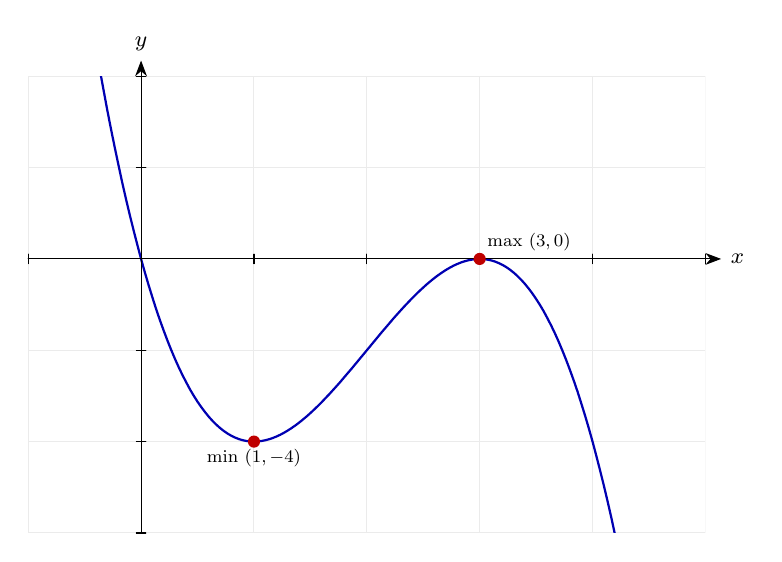
\begin{tikzpicture}[>={Stealth[length=2mm]},font=\footnotesize,line cap=round,line join=round]
\begin{scope}
\clip (0,0) rectangle (8.6,5.8);
\draw[gray!16] (0,0) grid[xstep=1.433,ystep=1.16] (8.6,5.8);
\draw[blue!70!black,thick] (0,11.6) -- (0.048,11.6) -- (0.096,11.6) -- (0.143,11.42) -- (0.191,10.995) -- (0.239,10.582) -- (0.287,10.18) -- (0.334,9.789) -- (0.382,9.408) -- (0.43,9.038) -- (0.478,8.679) -- (0.526,8.329) -- (0.573,7.99) -- (0.621,7.661) -- (0.669,7.342) -- (0.717,7.032) -- (0.764,6.733) -- (0.812,6.443) -- (0.86,6.162) -- (0.908,5.89) -- (0.956,5.628) -- (1.003,5.375) -- (1.051,5.13) -- (1.099,4.895) -- (1.147,4.668) -- (1.194,4.449) -- (1.242,4.239) -- (1.29,4.037) -- (1.338,3.844) -- (1.386,3.658) -- (1.433,3.48) -- (1.481,3.31) -- (1.529,3.147) -- (1.577,2.992) -- (1.624,2.844) -- (1.672,2.704) -- (1.72,2.571) -- (1.768,2.444) -- (1.816,2.324) -- (1.863,2.212) -- (1.911,2.105) -- (1.959,2.005) -- (2.007,1.912) -- (2.054,1.824) -- (2.102,1.743) -- (2.15,1.667) -- (2.198,1.598) -- (2.246,1.534) -- (2.293,1.476) -- (2.341,1.423) -- (2.389,1.375) -- (2.437,1.332) -- (2.484,1.295) -- (2.532,1.262) -- (2.58,1.234) -- (2.628,1.211) -- (2.676,1.192) -- (2.723,1.178) -- (2.771,1.168) -- (2.819,1.162) -- (2.867,1.16) -- (2.914,1.162) -- (2.962,1.168) -- (3.01,1.177) -- (3.058,1.19) -- (3.106,1.206) -- (3.153,1.225) -- (3.201,1.247) -- (3.249,1.273) -- (3.297,1.301) -- (3.344,1.332) -- (3.392,1.365) -- (3.44,1.401) -- (3.488,1.44) -- (3.536,1.48) -- (3.583,1.522) -- (3.631,1.567) -- (3.679,1.613) -- (3.727,1.661) -- (3.774,1.711) -- (3.822,1.761) -- (3.87,1.814) -- (3.918,1.867) -- (3.966,1.921) -- (4.013,1.977) -- (4.061,2.033) -- (4.109,2.089) -- (4.157,2.147) -- (4.204,2.204) -- (4.252,2.262) -- (4.3,2.32) -- (4.348,2.378) -- (4.396,2.436) -- (4.443,2.493) -- (4.491,2.551) -- (4.539,2.607) -- (4.587,2.663) -- (4.634,2.719) -- (4.682,2.773) -- (4.73,2.826) -- (4.778,2.879) -- (4.826,2.929) -- (4.873,2.979) -- (4.921,3.027) -- (4.969,3.073) -- (5.017,3.117) -- (5.064,3.16) -- (5.112,3.2) -- (5.16,3.239) -- (5.208,3.275) -- (5.256,3.308) -- (5.303,3.339) -- (5.351,3.367) -- (5.399,3.393) -- (5.447,3.415) -- (5.494,3.434) -- (5.542,3.45) -- (5.59,3.463) -- (5.638,3.472) -- (5.686,3.478) -- (5.733,3.48) -- (5.781,3.478) -- (5.829,3.472) -- (5.877,3.462) -- (5.924,3.448) -- (5.972,3.429) -- (6.02,3.406) -- (6.068,3.378) -- (6.116,3.345) -- (6.163,3.308) -- (6.211,3.265) -- (6.259,3.217) -- (6.307,3.164) -- (6.354,3.106) -- (6.402,3.042) -- (6.45,2.972) -- (6.498,2.897) -- (6.546,2.816) -- (6.593,2.728) -- (6.641,2.635) -- (6.689,2.535) -- (6.737,2.428) -- (6.784,2.316) -- (6.832,2.196) -- (6.88,2.069) -- (6.928,1.936) -- (6.976,1.796) -- (7.023,1.648) -- (7.071,1.493) -- (7.119,1.33) -- (7.167,1.16) -- (7.214,0.982) -- (7.262,0.796) -- (7.31,0.603) -- (7.358,0.401) -- (7.406,0.191) -- (7.453,-0.028) -- (7.501,-0.255) -- (7.549,-0.49) -- (7.597,-0.735) -- (7.644,-0.988) -- (7.692,-1.25) -- (7.74,-1.522) -- (7.788,-1.803) -- (7.836,-2.093) -- (7.883,-2.392) -- (7.931,-2.702) -- (7.979,-3.021) -- (8.027,-3.35) -- (8.074,-3.689) -- (8.122,-4.039) -- (8.17,-4.398) -- (8.218,-4.768) -- (8.266,-5.149) -- (8.313,-5.54) -- (8.361,-5.8) -- (8.409,-5.8) -- (8.457,-5.8) -- (8.504,-5.8) -- (8.552,-5.8) -- (8.6,-5.8);
\end{scope}
\draw[->] (0,3.48) -- (8.8,3.48) node[right]{$x$};
\draw[->] (1.433,0) -- (1.433,6) node[above]{$y$};
\draw (0,3.42) -- (0,3.54);
\draw (2.867,3.42) -- (2.867,3.54);
\draw (4.3,3.42) -- (4.3,3.54);
\draw (5.733,3.42) -- (5.733,3.54);
\draw (7.167,3.42) -- (7.167,3.54);
\draw (8.6,3.42) -- (8.6,3.54);
\draw (1.373,0) -- (1.493,0);
\draw (1.373,1.16) -- (1.493,1.16);
\draw (1.373,2.32) -- (1.493,2.32);
\draw (1.373,4.64) -- (1.493,4.64);
\draw (1.373,5.8) -- (1.493,5.8);
\fill[red!75!black] (2.867,1.16) circle (2.2pt);
\node[below,scale=0.8] at (2.867,1.16) {min $(1,-4)$};
\fill[red!75!black] (5.733,3.48) circle (2.2pt);
\node[above right,scale=0.8] at (5.733,3.48) {max $(3,0)$};
\end{tikzpicture}
}
\end{center}
\small Curve with classified stationary points marked.\normalsize

\medskip\hrule

\section*{Derivatives and Graphs 51\quad\small\texttt{(d4-051)}}
\addcontentsline{toc}{section}{Derivatives and Graphs 51 (d4-051)}
\textit{Difficulty: Standard \quad\textbar\quad Marks: 8}

\question{For the curve \( y = x^4 - 4x^2 + 3 \): (a) find the axis intercepts, (b) find and classify the stationary points.}

\textbf{Worked solution.}

\textit{Step 1: (a) Factorise as a biquadratic.}
\[\begin{gathered}
y = (x^2 - 1)(x^2 - 3) = (x-1)(x+1)(x - \sqrt{3})(x + \sqrt{3})
\end{gathered}\]
Let \( u = x^2 \) and factorise \( u^2 - 4u + 3 \).

\textit{Step 2: Intercepts.}
\[\begin{gathered}
\text{Roots: } x = \pm 1, \pm\sqrt{3}; \; y\text{-intercept} = 3
\end{gathered}\]
Four real roots.

\textit{Step 3: (b) Differentiate.}
\[\begin{gathered}
\frac{\mathrm{d}y}{\mathrm{d}x} = 4x^3 - 8x = 4x(x^2 - 2)
\end{gathered}\]
Factor out \( 4x \).

\textit{Step 4: Solve for stationary points.}
\[\begin{gathered}
x = 0 \text{ or } x = \pm\sqrt{2}
\end{gathered}\]
Three stationary points.

\textit{Step 5: Find \( y \) values.}
\[\begin{gathered}
y(0) = 3 \\ y(\pm\sqrt{2}) = 4 - 8 + 3 = -1
\end{gathered}\]
Substitute.

\textit{Step 6: Second derivative test.}
\[\begin{gathered}
y'' = 12x^2 - 8 \\ y''(0) = -8 < 0\; (\text{max}) \\ y''(\pm\sqrt{2}) = 16 > 0\; (\text{min})
\end{gathered}\]
Classify each.

\begin{answerbox}
\textbf{Final answer:}\quad (a) \(\displaystyle  (\pm 1, 0) \), \(\displaystyle  (\pm\sqrt{3}, 0) \), \(\displaystyle  (0, 3) \). \\[3pt]  (b) Maximum at \(\displaystyle  (0, 3) \); minima at \(\displaystyle  (\pm\sqrt{2}, -1) \).
\end{answerbox}
\textbf{Diagram.}

\begin{center}
\resizebox{\ifdim\width>\linewidth \linewidth\else \width\fi}{!}{%
\begin{tikzpicture}[>={Stealth[length=2mm]},font=\footnotesize,line cap=round,line join=round]
\begin{scope}
\clip (0,0) rectangle (8.6,5.8);
\draw[gray!16] (-0.86,0) grid[xstep=1.72,ystep=0.725] (8.6,5.8);
\draw[blue!70!black,thick] (0,11.6) -- (0.048,11.6) -- (0.096,11.6) -- (0.143,11.417) -- (0.191,10.687) -- (0.239,9.99) -- (0.287,9.327) -- (0.334,8.695) -- (0.382,8.095) -- (0.43,7.525) -- (0.478,6.984) -- (0.526,6.472) -- (0.573,5.989) -- (0.621,5.532) -- (0.669,5.101) -- (0.717,4.696) -- (0.764,4.315) -- (0.812,3.959) -- (0.86,3.625) -- (0.908,3.314) -- (0.956,3.024) -- (1.003,2.756) -- (1.051,2.507) -- (1.099,2.278) -- (1.147,2.068) -- (1.194,1.876) -- (1.242,1.701) -- (1.29,1.543) -- (1.338,1.402) -- (1.386,1.275) -- (1.433,1.164) -- (1.481,1.066) -- (1.529,0.982) -- (1.577,0.911) -- (1.624,0.853) -- (1.672,0.806) -- (1.72,0.77) -- (1.768,0.745) -- (1.816,0.73) -- (1.863,0.725) -- (1.911,0.729) -- (1.959,0.741) -- (2.007,0.761) -- (2.054,0.788) -- (2.102,0.823) -- (2.15,0.864) -- (2.198,0.911) -- (2.246,0.963) -- (2.293,1.021) -- (2.341,1.083) -- (2.389,1.15) -- (2.437,1.22) -- (2.484,1.294) -- (2.532,1.371) -- (2.58,1.45) -- (2.628,1.532) -- (2.676,1.615) -- (2.723,1.7) -- (2.771,1.786) -- (2.819,1.873) -- (2.867,1.961) -- (2.914,2.048) -- (2.962,2.136) -- (3.01,2.223) -- (3.058,2.31) -- (3.106,2.395) -- (3.153,2.479) -- (3.201,2.562) -- (3.249,2.643) -- (3.297,2.722) -- (3.344,2.799) -- (3.392,2.873) -- (3.44,2.945) -- (3.488,3.014) -- (3.536,3.08) -- (3.583,3.143) -- (3.631,3.203) -- (3.679,3.259) -- (3.727,3.312) -- (3.774,3.361) -- (3.822,3.406) -- (3.87,3.447) -- (3.918,3.484) -- (3.966,3.516) -- (4.013,3.545) -- (4.061,3.569) -- (4.109,3.589) -- (4.157,3.605) -- (4.204,3.616) -- (4.252,3.623) -- (4.3,3.625) -- (4.348,3.623) -- (4.396,3.616) -- (4.443,3.605) -- (4.491,3.589) -- (4.539,3.569) -- (4.587,3.545) -- (4.634,3.516) -- (4.682,3.484) -- (4.73,3.447) -- (4.778,3.406) -- (4.826,3.361) -- (4.873,3.312) -- (4.921,3.259) -- (4.969,3.203) -- (5.017,3.143) -- (5.064,3.08) -- (5.112,3.014) -- (5.16,2.945) -- (5.208,2.873) -- (5.256,2.799) -- (5.303,2.722) -- (5.351,2.643) -- (5.399,2.562) -- (5.447,2.479) -- (5.494,2.395) -- (5.542,2.31) -- (5.59,2.223) -- (5.638,2.136) -- (5.686,2.048) -- (5.733,1.961) -- (5.781,1.873) -- (5.829,1.786) -- (5.877,1.7) -- (5.924,1.615) -- (5.972,1.532) -- (6.02,1.45) -- (6.068,1.371) -- (6.116,1.294) -- (6.163,1.22) -- (6.211,1.15) -- (6.259,1.083) -- (6.307,1.021) -- (6.354,0.963) -- (6.402,0.911) -- (6.45,0.864) -- (6.498,0.823) -- (6.546,0.788) -- (6.593,0.761) -- (6.641,0.741) -- (6.689,0.729) -- (6.737,0.725) -- (6.784,0.73) -- (6.832,0.745) -- (6.88,0.77) -- (6.928,0.806) -- (6.976,0.853) -- (7.023,0.911) -- (7.071,0.982) -- (7.119,1.066) -- (7.167,1.164) -- (7.214,1.275) -- (7.262,1.402) -- (7.31,1.543) -- (7.358,1.701) -- (7.406,1.876) -- (7.453,2.068) -- (7.501,2.278) -- (7.549,2.507) -- (7.597,2.756) -- (7.644,3.024) -- (7.692,3.314) -- (7.74,3.625) -- (7.788,3.959) -- (7.836,4.315) -- (7.883,4.696) -- (7.931,5.101) -- (7.979,5.532) -- (8.027,5.989) -- (8.074,6.472) -- (8.122,6.984) -- (8.17,7.525) -- (8.218,8.095) -- (8.266,8.695) -- (8.313,9.327) -- (8.361,9.99) -- (8.409,10.687) -- (8.457,11.417) -- (8.504,11.6) -- (8.552,11.6) -- (8.6,11.6);
\end{scope}
\draw[->] (0,1.45) -- (8.8,1.45) node[right]{$x$};
\draw[->] (4.3,0) -- (4.3,6) node[above]{$y$};
\draw (0.86,1.39) -- (0.86,1.51);
\draw (2.58,1.39) -- (2.58,1.51);
\draw (6.02,1.39) -- (6.02,1.51);
\draw (7.74,1.39) -- (7.74,1.51);
\draw (4.24,0) -- (4.36,0);
\draw (4.24,0.725) -- (4.36,0.725);
\draw (4.24,2.175) -- (4.36,2.175);
\draw (4.24,2.9) -- (4.36,2.9);
\draw (4.24,3.625) -- (4.36,3.625);
\draw (4.24,4.35) -- (4.36,4.35);
\draw (4.24,5.075) -- (4.36,5.075);
\draw (4.24,5.8) -- (4.36,5.8);
\fill[red!75!black] (4.3,3.625) circle (2.2pt);
\node[above,scale=0.8] at (4.3,3.625) {max $(0,3)$};
\fill[red!75!black] (6.732,0.725) circle (2.2pt);
\node[below,scale=0.8] at (6.732,0.725) {min};
\fill[red!75!black] (1.868,0.725) circle (2.2pt);
\node[below,scale=0.8] at (1.868,0.725) {min};
\end{tikzpicture}
}
\end{center}
\small Curve with classified stationary points marked.\normalsize

\medskip\hrule

\section*{Derivatives and Graphs 52\quad\small\texttt{(d4-052)}}
\addcontentsline{toc}{section}{Derivatives and Graphs 52 (d4-052)}
\textit{Difficulty: Standard \quad\textbar\quad Marks: 8}

\question{Sketch the curve \( y = x^3 - 3x^2 + 4 \), labelling intercepts and stationary points.}

\textbf{Worked solution.}

\textit{Step 1: \( y \)-intercept.}
\[\begin{gathered}
y(0) = 4
\end{gathered}\]
\( (0, 4) \).

\textit{Step 2: Try \( x = -1 \) as a root.}
\[\begin{gathered}
y(-1) = -1 - 3 + 4 = 0 \Rightarrow (x + 1) \text{ is a factor}
\end{gathered}\]
Factor theorem.

\textit{Step 3: Divide to factorise.}
\[\begin{gathered}
y = (x + 1)(x^2 - 4x + 4) = (x + 1)(x - 2)^2
\end{gathered}\]
Perfect square in the quadratic.

\textit{Step 4: \( x \)-intercepts.}
\[\begin{gathered}
x = -1 \text{ (crosses)},\; x = 2 \text{ (touches)}
\end{gathered}\]
\( (x - 2)^2 \) means the curve touches.

\textit{Step 5: Differentiate.}
\[\begin{gathered}
\frac{\mathrm{d}y}{\mathrm{d}x} = 3x^2 - 6x = 3x(x - 2)
\end{gathered}\]
Factorise.

\textit{Step 6: Stationary points.}
\[\begin{gathered}
x = 0: \; y = 4 \\ x = 2: \; y = 0
\end{gathered}\]
Substitute.

\textit{Step 7: Classify.}
\[\begin{gathered}
y'' = 6x - 6 \\ y''(0) = -6 < 0\; (\text{max}) \\ y''(2) = 6 > 0\; (\text{min})
\end{gathered}\]
Second derivative test.

\begin{answerbox}
\textbf{Final answer:}\quad Intercepts: \(\displaystyle  (-1, 0) \), \(\displaystyle  (2, 0) \), \(\displaystyle  (0, 4) \). Maximum at \(\displaystyle  (0, 4) \); minimum at \(\displaystyle  (2, 0) \).
\end{answerbox}
\textbf{Diagram.}

\begin{center}
\resizebox{\ifdim\width>\linewidth \linewidth\else \width\fi}{!}{%
\begin{tikzpicture}[>={Stealth[length=2mm]},font=\footnotesize,line cap=round,line join=round]
\begin{scope}
\clip (0,0) rectangle (8.6,5.8);
\draw[gray!16] (0,0) grid[xstep=1.229,ystep=1.16] (8.6,5.8);
\draw[blue!70!black,thick] (0,-5.8) -- (0.048,-5.8) -- (0.096,-5.8) -- (0.143,-5.8) -- (0.191,-5.8) -- (0.239,-5.8) -- (0.287,-5.8) -- (0.334,-5.8) -- (0.382,-5.8) -- (0.43,-5.8) -- (0.478,-5.8) -- (0.526,-5.8) -- (0.573,-5.8) -- (0.621,-5.8) -- (0.669,-5.8) -- (0.717,-5.8) -- (0.764,-5.8) -- (0.812,-5.8) -- (0.86,-5.8) -- (0.908,-5.8) -- (0.956,-5.8) -- (1.003,-5.8) -- (1.051,-5.8) -- (1.099,-5.8) -- (1.147,-5.8) -- (1.194,-5.8) -- (1.242,-5.8) -- (1.29,-5.8) -- (1.338,-5.8) -- (1.386,-5.8) -- (1.433,-5.8) -- (1.481,-5.474) -- (1.529,-5.021) -- (1.577,-4.582) -- (1.624,-4.157) -- (1.672,-3.747) -- (1.72,-3.35) -- (1.768,-2.967) -- (1.816,-2.598) -- (1.863,-2.241) -- (1.911,-1.898) -- (1.959,-1.568) -- (2.007,-1.25) -- (2.054,-0.945) -- (2.102,-0.652) -- (2.15,-0.372) -- (2.198,-0.103) -- (2.246,0.155) -- (2.293,0.401) -- (2.341,0.635) -- (2.389,0.859) -- (2.437,1.072) -- (2.484,1.274) -- (2.532,1.466) -- (2.58,1.648) -- (2.628,1.819) -- (2.676,1.981) -- (2.723,2.134) -- (2.771,2.276) -- (2.819,2.41) -- (2.867,2.535) -- (2.914,2.651) -- (2.962,2.758) -- (3.01,2.857) -- (3.058,2.948) -- (3.106,3.031) -- (3.153,3.106) -- (3.201,3.174) -- (3.249,3.234) -- (3.297,3.287) -- (3.344,3.333) -- (3.392,3.373) -- (3.44,3.406) -- (3.488,3.432) -- (3.536,3.453) -- (3.583,3.468) -- (3.631,3.477) -- (3.679,3.48) -- (3.727,3.478) -- (3.774,3.471) -- (3.822,3.459) -- (3.87,3.443) -- (3.918,3.422) -- (3.966,3.397) -- (4.013,3.367) -- (4.061,3.334) -- (4.109,3.297) -- (4.157,3.257) -- (4.204,3.213) -- (4.252,3.167) -- (4.3,3.117) -- (4.348,3.065) -- (4.396,3.011) -- (4.443,2.954) -- (4.491,2.896) -- (4.539,2.835) -- (4.587,2.773) -- (4.634,2.709) -- (4.682,2.645) -- (4.73,2.579) -- (4.778,2.513) -- (4.826,2.445) -- (4.873,2.378) -- (4.921,2.31) -- (4.969,2.243) -- (5.017,2.175) -- (5.064,2.108) -- (5.112,2.042) -- (5.16,1.977) -- (5.208,1.912) -- (5.256,1.849) -- (5.303,1.787) -- (5.351,1.727) -- (5.399,1.669) -- (5.447,1.613) -- (5.494,1.559) -- (5.542,1.508) -- (5.59,1.459) -- (5.638,1.414) -- (5.686,1.371) -- (5.733,1.332) -- (5.781,1.296) -- (5.829,1.264) -- (5.877,1.236) -- (5.924,1.212) -- (5.972,1.192) -- (6.02,1.177) -- (6.068,1.166) -- (6.116,1.161) -- (6.163,1.16) -- (6.211,1.165) -- (6.259,1.176) -- (6.307,1.192) -- (6.354,1.215) -- (6.402,1.243) -- (6.45,1.278) -- (6.498,1.319) -- (6.546,1.367) -- (6.593,1.423) -- (6.641,1.485) -- (6.689,1.555) -- (6.737,1.632) -- (6.784,1.717) -- (6.832,1.81) -- (6.88,1.912) -- (6.928,2.021) -- (6.976,2.14) -- (7.023,2.267) -- (7.071,2.403) -- (7.119,2.549) -- (7.167,2.704) -- (7.214,2.869) -- (7.262,3.043) -- (7.31,3.228) -- (7.358,3.422) -- (7.406,3.628) -- (7.453,3.844) -- (7.501,4.07) -- (7.549,4.308) -- (7.597,4.558) -- (7.644,4.818) -- (7.692,5.091) -- (7.74,5.375) -- (7.788,5.671) -- (7.836,5.98) -- (7.883,6.301) -- (7.931,6.635) -- (7.979,6.982) -- (8.027,7.342) -- (8.074,7.715) -- (8.122,8.102) -- (8.17,8.503) -- (8.218,8.917) -- (8.266,9.346) -- (8.313,9.789) -- (8.361,10.246) -- (8.409,10.719) -- (8.457,11.206) -- (8.504,11.6) -- (8.552,11.6) -- (8.6,11.6);
\end{scope}
\draw[->] (0,1.16) -- (8.8,1.16) node[right]{$x$};
\draw[->] (3.686,0) -- (3.686,6) node[above]{$y$};
\draw (0,1.1) -- (0,1.22);
\draw (1.229,1.1) -- (1.229,1.22);
\draw (2.457,1.1) -- (2.457,1.22);
\draw (4.914,1.1) -- (4.914,1.22);
\draw (6.143,1.1) -- (6.143,1.22);
\draw (7.371,1.1) -- (7.371,1.22);
\draw (8.6,1.1) -- (8.6,1.22);
\draw (3.626,0) -- (3.746,0);
\draw (3.626,2.32) -- (3.746,2.32);
\draw (3.626,3.48) -- (3.746,3.48);
\draw (3.626,4.64) -- (3.746,4.64);
\draw (3.626,5.8) -- (3.746,5.8);
\fill[red!75!black] (3.686,3.48) circle (2.2pt);
\node[above,scale=0.8] at (3.686,3.48) {max $(0,4)$};
\fill[red!75!black] (6.143,1.16) circle (2.2pt);
\node[below right,scale=0.8] at (6.143,1.16) {min $(2,0)$};
\fill[red!75!black] (2.457,1.16) circle (2.2pt);
\node[below left,scale=0.8] at (2.457,1.16) {$-1$};
\end{tikzpicture}
}
\end{center}
\small Curve with classified stationary points marked.\normalsize

\medskip\hrule

\section*{Derivatives and Graphs 53\quad\small\texttt{(d4-053)}}
\addcontentsline{toc}{section}{Derivatives and Graphs 53 (d4-053)}
\textit{Difficulty: Standard \quad\textbar\quad Marks: 7}

\question{For \( y = x^4 - 2x^2 \): (a) find the \( x \)-intercepts, (b) find and classify all stationary points.}

\textbf{Worked solution.}

\textit{Step 1: (a) Factorise.}
\[\begin{gathered}
y = x^2(x^2 - 2) = x^2(x - \sqrt{2})(x + \sqrt{2})
\end{gathered}\]
Factor out \( x^2 \), then difference of squares.

\textit{Step 2: Intercepts.}
\[\begin{gathered}
x = 0 \text{ (double)},\; x = \pm\sqrt{2}
\end{gathered}\]
Touches at origin, crosses at \( \pm\sqrt{2} \).

\textit{Step 3: (b) Differentiate.}
\[\begin{gathered}
\frac{\mathrm{d}y}{\mathrm{d}x} = 4x^3 - 4x = 4x(x^2 - 1) = 4x(x - 1)(x + 1)
\end{gathered}\]
Factorise.

\textit{Step 4: Stationary points.}
\[\begin{gathered}
x = 0: \; y = 0 \\ x = \pm 1: \; y = 1 - 2 = -1
\end{gathered}\]
Substitute.

\textit{Step 5: Second derivative test.}
\[\begin{gathered}
y'' = 12x^2 - 4 \\ y''(0) = -4 < 0\; (\text{max}) \\ y''(\pm 1) = 8 > 0\; (\text{min})
\end{gathered}\]
Classify each.

\begin{answerbox}
\textbf{Final answer:}\quad (a) \(\displaystyle  (0, 0), (\pm\sqrt{2}, 0) \). \\[3pt]  (b) Maximum at \(\displaystyle  (0, 0) \); minima at \(\displaystyle  (\pm 1, -1) \).
\end{answerbox}
\textbf{Diagram.}

\begin{center}
\resizebox{\ifdim\width>\linewidth \linewidth\else \width\fi}{!}{%
\begin{tikzpicture}[>={Stealth[length=2mm]},font=\footnotesize,line cap=round,line join=round]
\begin{scope}
\clip (0,0) rectangle (8.6,5.8);
\draw[gray!16] (0,0) grid[xstep=1.075,ystep=0.967] (8.6,5.8);
\draw[blue!70!black,thick] (0,9.667) -- (0.048,9.162) -- (0.096,8.677) -- (0.143,8.212) -- (0.191,7.767) -- (0.239,7.341) -- (0.287,6.933) -- (0.334,6.544) -- (0.382,6.172) -- (0.43,5.817) -- (0.478,5.479) -- (0.526,5.157) -- (0.573,4.851) -- (0.621,4.56) -- (0.669,4.283) -- (0.717,4.022) -- (0.764,3.774) -- (0.812,3.54) -- (0.86,3.319) -- (0.908,3.111) -- (0.956,2.915) -- (1.003,2.731) -- (1.051,2.559) -- (1.099,2.398) -- (1.147,2.248) -- (1.194,2.108) -- (1.242,1.978) -- (1.29,1.858) -- (1.338,1.747) -- (1.386,1.645) -- (1.433,1.551) -- (1.481,1.466) -- (1.529,1.389) -- (1.577,1.32) -- (1.624,1.258) -- (1.672,1.202) -- (1.72,1.154) -- (1.768,1.112) -- (1.816,1.075) -- (1.863,1.045) -- (1.911,1.02) -- (1.959,1) -- (2.007,0.985) -- (2.054,0.975) -- (2.102,0.969) -- (2.15,0.967) -- (2.198,0.969) -- (2.246,0.974) -- (2.293,0.983) -- (2.341,0.995) -- (2.389,1.009) -- (2.437,1.027) -- (2.484,1.046) -- (2.532,1.068) -- (2.58,1.092) -- (2.628,1.118) -- (2.676,1.145) -- (2.723,1.173) -- (2.771,1.203) -- (2.819,1.234) -- (2.867,1.265) -- (2.914,1.297) -- (2.962,1.33) -- (3.01,1.363) -- (3.058,1.396) -- (3.106,1.429) -- (3.153,1.462) -- (3.201,1.494) -- (3.249,1.526) -- (3.297,1.558) -- (3.344,1.589) -- (3.392,1.619) -- (3.44,1.649) -- (3.488,1.677) -- (3.536,1.704) -- (3.583,1.73) -- (3.631,1.755) -- (3.679,1.779) -- (3.727,1.801) -- (3.774,1.821) -- (3.822,1.84) -- (3.87,1.858) -- (3.918,1.873) -- (3.966,1.887) -- (4.013,1.899) -- (4.061,1.91) -- (4.109,1.918) -- (4.157,1.925) -- (4.204,1.93) -- (4.252,1.932) -- (4.3,1.933) -- (4.348,1.932) -- (4.396,1.93) -- (4.443,1.925) -- (4.491,1.918) -- (4.539,1.91) -- (4.587,1.899) -- (4.634,1.887) -- (4.682,1.873) -- (4.73,1.858) -- (4.778,1.84) -- (4.826,1.821) -- (4.873,1.801) -- (4.921,1.779) -- (4.969,1.755) -- (5.017,1.73) -- (5.064,1.704) -- (5.112,1.677) -- (5.16,1.649) -- (5.208,1.619) -- (5.256,1.589) -- (5.303,1.558) -- (5.351,1.526) -- (5.399,1.494) -- (5.447,1.462) -- (5.494,1.429) -- (5.542,1.396) -- (5.59,1.363) -- (5.638,1.33) -- (5.686,1.297) -- (5.733,1.265) -- (5.781,1.234) -- (5.829,1.203) -- (5.877,1.173) -- (5.924,1.145) -- (5.972,1.118) -- (6.02,1.092) -- (6.068,1.068) -- (6.116,1.046) -- (6.163,1.027) -- (6.211,1.009) -- (6.259,0.995) -- (6.307,0.983) -- (6.354,0.974) -- (6.402,0.969) -- (6.45,0.967) -- (6.498,0.969) -- (6.546,0.975) -- (6.593,0.985) -- (6.641,1) -- (6.689,1.02) -- (6.737,1.045) -- (6.784,1.075) -- (6.832,1.112) -- (6.88,1.154) -- (6.928,1.202) -- (6.976,1.258) -- (7.023,1.32) -- (7.071,1.389) -- (7.119,1.466) -- (7.167,1.551) -- (7.214,1.645) -- (7.262,1.747) -- (7.31,1.858) -- (7.358,1.978) -- (7.406,2.108) -- (7.453,2.248) -- (7.501,2.398) -- (7.549,2.559) -- (7.597,2.731) -- (7.644,2.915) -- (7.692,3.111) -- (7.74,3.319) -- (7.788,3.54) -- (7.836,3.774) -- (7.883,4.022) -- (7.931,4.283) -- (7.979,4.56) -- (8.027,4.851) -- (8.074,5.157) -- (8.122,5.479) -- (8.17,5.817) -- (8.218,6.172) -- (8.266,6.544) -- (8.313,6.933) -- (8.361,7.341) -- (8.409,7.767) -- (8.457,8.212) -- (8.504,8.677) -- (8.552,9.162) -- (8.6,9.667);
\end{scope}
\draw[->] (0,1.933) -- (8.8,1.933) node[right]{$x$};
\draw[->] (4.3,0) -- (4.3,6) node[above]{$y$};
\draw (0,1.873) -- (0,1.993);
\draw (1.075,1.873) -- (1.075,1.993);
\draw (2.15,1.873) -- (2.15,1.993);
\draw (3.225,1.873) -- (3.225,1.993);
\draw (5.375,1.873) -- (5.375,1.993);
\draw (6.45,1.873) -- (6.45,1.993);
\draw (7.525,1.873) -- (7.525,1.993);
\draw (8.6,1.873) -- (8.6,1.993);
\draw (4.24,0) -- (4.36,0);
\draw (4.24,0.967) -- (4.36,0.967);
\draw (4.24,2.9) -- (4.36,2.9);
\draw (4.24,3.867) -- (4.36,3.867);
\draw (4.24,4.833) -- (4.36,4.833);
\draw (4.24,5.8) -- (4.36,5.8);
\fill[red!75!black] (4.3,1.933) circle (2.2pt);
\node[above,scale=0.8] at (4.3,1.933) {max $(0,0)$};
\fill[red!75!black] (6.45,0.967) circle (2.2pt);
\node[below,scale=0.8] at (6.45,0.967) {min};
\fill[red!75!black] (2.15,0.967) circle (2.2pt);
\node[below,scale=0.8] at (2.15,0.967) {min};
\end{tikzpicture}
}
\end{center}
\small Curve with classified stationary points marked.\normalsize

\medskip\hrule

\section*{Derivatives and Graphs 54\quad\small\texttt{(d4-054)}}
\addcontentsline{toc}{section}{Derivatives and Graphs 54 (d4-054)}
\textit{Difficulty: Standard \quad\textbar\quad Marks: 8}

\question{Sketch \( y = x^3 - 12x + 16 \), labelling any stationary points and the \( y \)-intercept. Determine the nature of each stationary point.}

\textbf{Worked solution.}

\textit{Step 1: \( y \)-intercept.}
\[\begin{gathered}
y(0) = 16
\end{gathered}\]
\( (0, 16) \).

\textit{Step 2: Differentiate.}
\[\begin{gathered}
\frac{\mathrm{d}y}{\mathrm{d}x} = 3x^2 - 12 = 3(x - 2)(x + 2)
\end{gathered}\]
Factorise.

\textit{Step 3: Stationary points.}
\[\begin{gathered}
x = 2: \; y = 8 - 24 + 16 = 0 \\ x = -2: \; y = -8 + 24 + 16 = 32
\end{gathered}\]
Substitute.

\textit{Step 4: Classify.}
\[\begin{gathered}
y'' = 6x \\ y''(2) = 12 > 0\; (\text{min}) \\ y''(-2) = -12 < 0\; (\text{max})
\end{gathered}\]
Second derivative test.

\begin{answerbox}
\textbf{Final answer:}\quad Maximum at \(\displaystyle  (-2, 32) \); minimum at \(\displaystyle  (2, 0) \); \(\displaystyle  y \)-intercept \(\displaystyle  (0, 16) \).
\end{answerbox}
\textbf{Diagram.}

\begin{center}
\resizebox{\ifdim\width>\linewidth \linewidth\else \width\fi}{!}{%
\begin{tikzpicture}[>={Stealth[length=2mm]},font=\footnotesize,line cap=round,line join=round]
\begin{scope}
\clip (0,0) rectangle (8.6,5.8);
\draw[gray!16] (0,-0.644) grid[xstep=1.075,ystep=1.289] (8.6,5.8);
\draw[blue!70!black,thick] (0,0.644) -- (0.048,0.848) -- (0.096,1.045) -- (0.143,1.236) -- (0.191,1.421) -- (0.239,1.601) -- (0.287,1.774) -- (0.334,1.942) -- (0.382,2.104) -- (0.43,2.261) -- (0.478,2.412) -- (0.526,2.558) -- (0.573,2.699) -- (0.621,2.834) -- (0.669,2.964) -- (0.717,3.089) -- (0.764,3.208) -- (0.812,3.323) -- (0.86,3.433) -- (0.908,3.537) -- (0.956,3.637) -- (1.003,3.733) -- (1.051,3.823) -- (1.099,3.909) -- (1.147,3.99) -- (1.194,4.067) -- (1.242,4.14) -- (1.29,4.208) -- (1.338,4.272) -- (1.386,4.331) -- (1.433,4.387) -- (1.481,4.438) -- (1.529,4.486) -- (1.577,4.529) -- (1.624,4.569) -- (1.672,4.605) -- (1.72,4.637) -- (1.768,4.665) -- (1.816,4.69) -- (1.863,4.711) -- (1.911,4.729) -- (1.959,4.744) -- (2.007,4.755) -- (2.054,4.763) -- (2.102,4.767) -- (2.15,4.769) -- (2.198,4.767) -- (2.246,4.763) -- (2.293,4.755) -- (2.341,4.745) -- (2.389,4.732) -- (2.437,4.716) -- (2.484,4.698) -- (2.532,4.677) -- (2.58,4.653) -- (2.628,4.627) -- (2.676,4.599) -- (2.723,4.568) -- (2.771,4.536) -- (2.819,4.501) -- (2.867,4.463) -- (2.914,4.424) -- (2.962,4.383) -- (3.01,4.34) -- (3.058,4.295) -- (3.106,4.248) -- (3.153,4.2) -- (3.201,4.15) -- (3.249,4.098) -- (3.297,4.045) -- (3.344,3.991) -- (3.392,3.935) -- (3.44,3.878) -- (3.488,3.82) -- (3.536,3.76) -- (3.583,3.7) -- (3.631,3.638) -- (3.679,3.575) -- (3.727,3.512) -- (3.774,3.448) -- (3.822,3.383) -- (3.87,3.317) -- (3.918,3.251) -- (3.966,3.184) -- (4.013,3.117) -- (4.061,3.049) -- (4.109,2.981) -- (4.157,2.913) -- (4.204,2.844) -- (4.252,2.775) -- (4.3,2.707) -- (4.348,2.638) -- (4.396,2.569) -- (4.443,2.501) -- (4.491,2.432) -- (4.539,2.364) -- (4.587,2.297) -- (4.634,2.229) -- (4.682,2.163) -- (4.73,2.096) -- (4.778,2.031) -- (4.826,1.966) -- (4.873,1.901) -- (4.921,1.838) -- (4.969,1.775) -- (5.017,1.714) -- (5.064,1.653) -- (5.112,1.594) -- (5.16,1.535) -- (5.208,1.478) -- (5.256,1.422) -- (5.303,1.368) -- (5.351,1.315) -- (5.399,1.263) -- (5.447,1.213) -- (5.494,1.165) -- (5.542,1.118) -- (5.59,1.073) -- (5.638,1.03) -- (5.686,0.989) -- (5.733,0.95) -- (5.781,0.913) -- (5.829,0.878) -- (5.877,0.845) -- (5.924,0.814) -- (5.972,0.786) -- (6.02,0.76) -- (6.068,0.736) -- (6.116,0.715) -- (6.163,0.697) -- (6.211,0.681) -- (6.259,0.668) -- (6.307,0.658) -- (6.354,0.65) -- (6.402,0.646) -- (6.45,0.644) -- (6.498,0.646) -- (6.546,0.651) -- (6.593,0.658) -- (6.641,0.67) -- (6.689,0.684) -- (6.737,0.702) -- (6.784,0.723) -- (6.832,0.748) -- (6.88,0.776) -- (6.928,0.809) -- (6.976,0.844) -- (7.023,0.884) -- (7.071,0.927) -- (7.119,0.975) -- (7.167,1.026) -- (7.214,1.082) -- (7.262,1.142) -- (7.31,1.205) -- (7.358,1.274) -- (7.406,1.346) -- (7.453,1.423) -- (7.501,1.504) -- (7.549,1.59) -- (7.597,1.681) -- (7.644,1.776) -- (7.692,1.876) -- (7.74,1.981) -- (7.788,2.09) -- (7.836,2.205) -- (7.883,2.325) -- (7.931,2.45) -- (7.979,2.579) -- (8.027,2.715) -- (8.074,2.855) -- (8.122,3.001) -- (8.17,3.152) -- (8.218,3.309) -- (8.266,3.471) -- (8.313,3.639) -- (8.361,3.813) -- (8.409,3.992) -- (8.457,4.177) -- (8.504,4.369) -- (8.552,4.566) -- (8.6,4.769);
\end{scope}
\draw[->] (0,0.644) -- (8.8,0.644) node[right]{$x$};
\draw[->] (4.3,0) -- (4.3,6) node[above]{$y$};
\draw (0,0.584) -- (0,0.704);
\draw (1.075,0.584) -- (1.075,0.704);
\draw (2.15,0.584) -- (2.15,0.704);
\draw (3.225,0.584) -- (3.225,0.704);
\draw (5.375,0.584) -- (5.375,0.704);
\draw (6.45,0.584) -- (6.45,0.704);
\draw (7.525,0.584) -- (7.525,0.704);
\draw (8.6,0.584) -- (8.6,0.704);
\draw (4.24,1.933) -- (4.36,1.933);
\draw (4.24,3.222) -- (4.36,3.222);
\draw (4.24,4.511) -- (4.36,4.511);
\draw (4.24,5.8) -- (4.36,5.8);
\fill[red!75!black] (2.15,4.769) circle (2.2pt);
\node[above,scale=0.8] at (2.15,4.769) {max $(-2,32)$};
\fill[red!75!black] (6.45,0.644) circle (2.2pt);
\node[below right,scale=0.8] at (6.45,0.644) {min $(2,0)$};
\fill[red!75!black] (4.3,2.707) circle (2.2pt);
\node[right,scale=0.8] at (4.3,2.707) {$(0,16)$};
\end{tikzpicture}
}
\end{center}
\small Curve with classified stationary points marked.\normalsize

\medskip\hrule

\section*{Derivatives and Graphs 55\quad\small\texttt{(d4-055)}}
\addcontentsline{toc}{section}{Derivatives and Graphs 55 (d4-055)}
\textit{Difficulty: Standard \quad\textbar\quad Marks: 5}

\question{The curve \( y = x^3 + ax^2 + bx \) has a stationary point at \( x = -1 \) and passes through \( (2, 6) \). Find \( a \) and \( b \).}

\textbf{Worked solution.}

\textit{Step 1: Differentiate.}
\[\begin{gathered}
\frac{\mathrm{d}y}{\mathrm{d}x} = 3x^2 + 2ax + b
\end{gathered}\]
Apply the power rule.

\textit{Step 2: Stationary at \( x = -1 \): \( y'(-1) = 0 \).}
\[\begin{gathered}
3 - 2a + b = 0
\end{gathered}\]
First equation.

\textit{Step 3: Curve passes through \( (2, 6) \).}
\[\begin{gathered}
8 + 4a + 2b = 6 \Rightarrow 4a + 2b = -2 \Rightarrow 2a + b = -1
\end{gathered}\]
Second equation.

\textit{Step 4: Solve the system.}
\[\begin{gathered}
\begin{cases} -2a + b = -3 \\ 2a + b = -1 \end{cases} \Rightarrow 2b = -4 \Rightarrow b = -2
\end{gathered}\]
Add the two equations.

\textit{Step 5: Find \( a \).}
\[\begin{gathered}
2a - 2 = -1 \Rightarrow a = \tfrac{1}{2}
\end{gathered}\]
Substitute back.

\begin{answerbox}
\textbf{Final answer:}\quad \(\displaystyle  a = \dfrac{1}{2},\; b = -2 \).
\end{answerbox}
\textbf{Diagram.}

\begin{center}
\resizebox{\ifdim\width>\linewidth \linewidth\else \width\fi}{!}{%
\begin{tikzpicture}[>={Stealth[length=2mm]},font=\footnotesize,line cap=round,line join=round]
\begin{scope}
\clip (0,0) rectangle (8.6,5.8);
\draw[gray!16] (0,-0.58) grid[xstep=1.433,ystep=1.16] (8.6,5.8);
\draw[blue!70!black,thick] (0,-5.8) -- (0.048,-5.8) -- (0.096,-5.8) -- (0.143,-5.443) -- (0.191,-5.055) -- (0.239,-4.678) -- (0.287,-4.311) -- (0.334,-3.954) -- (0.382,-3.607) -- (0.43,-3.27) -- (0.478,-2.943) -- (0.526,-2.626) -- (0.573,-2.318) -- (0.621,-2.019) -- (0.669,-1.73) -- (0.717,-1.45) -- (0.764,-1.179) -- (0.812,-0.917) -- (0.86,-0.664) -- (0.908,-0.419) -- (0.956,-0.183) -- (1.003,0.045) -- (1.051,0.265) -- (1.099,0.476) -- (1.147,0.68) -- (1.194,0.875) -- (1.242,1.063) -- (1.29,1.244) -- (1.338,1.416) -- (1.386,1.582) -- (1.433,1.74) -- (1.481,1.891) -- (1.529,2.035) -- (1.577,2.173) -- (1.624,2.303) -- (1.672,2.427) -- (1.72,2.545) -- (1.768,2.656) -- (1.816,2.761) -- (1.863,2.861) -- (1.911,2.954) -- (1.959,3.041) -- (2.007,3.123) -- (2.054,3.199) -- (2.102,3.27) -- (2.15,3.335) -- (2.198,3.395) -- (2.246,3.451) -- (2.293,3.501) -- (2.341,3.546) -- (2.389,3.587) -- (2.437,3.624) -- (2.484,3.656) -- (2.532,3.684) -- (2.58,3.707) -- (2.628,3.727) -- (2.676,3.743) -- (2.723,3.755) -- (2.771,3.763) -- (2.819,3.768) -- (2.867,3.77) -- (2.914,3.768) -- (2.962,3.764) -- (3.01,3.756) -- (3.058,3.746) -- (3.106,3.732) -- (3.153,3.717) -- (3.201,3.698) -- (3.249,3.678) -- (3.297,3.655) -- (3.344,3.63) -- (3.392,3.604) -- (3.44,3.575) -- (3.488,3.545) -- (3.536,3.513) -- (3.583,3.48) -- (3.631,3.446) -- (3.679,3.41) -- (3.727,3.373) -- (3.774,3.336) -- (3.822,3.297) -- (3.87,3.258) -- (3.918,3.219) -- (3.966,3.179) -- (4.013,3.139) -- (4.061,3.099) -- (4.109,3.058) -- (4.157,3.018) -- (4.204,2.978) -- (4.252,2.939) -- (4.3,2.9) -- (4.348,2.862) -- (4.396,2.824) -- (4.443,2.787) -- (4.491,2.752) -- (4.539,2.717) -- (4.587,2.684) -- (4.634,2.652) -- (4.682,2.622) -- (4.73,2.594) -- (4.778,2.567) -- (4.826,2.542) -- (4.873,2.52) -- (4.921,2.499) -- (4.969,2.481) -- (5.017,2.465) -- (5.064,2.452) -- (5.112,2.441) -- (5.16,2.434) -- (5.208,2.429) -- (5.256,2.427) -- (5.303,2.429) -- (5.351,2.434) -- (5.399,2.442) -- (5.447,2.455) -- (5.494,2.47) -- (5.542,2.49) -- (5.59,2.514) -- (5.638,2.542) -- (5.686,2.574) -- (5.733,2.61) -- (5.781,2.651) -- (5.829,2.697) -- (5.877,2.747) -- (5.924,2.802) -- (5.972,2.862) -- (6.02,2.928) -- (6.068,2.999) -- (6.116,3.075) -- (6.163,3.156) -- (6.211,3.244) -- (6.259,3.337) -- (6.307,3.436) -- (6.354,3.541) -- (6.402,3.652) -- (6.45,3.77) -- (6.498,3.894) -- (6.546,4.025) -- (6.593,4.162) -- (6.641,4.306) -- (6.689,4.457) -- (6.737,4.616) -- (6.784,4.781) -- (6.832,4.954) -- (6.88,5.134) -- (6.928,5.322) -- (6.976,5.518) -- (7.023,5.721) -- (7.071,5.933) -- (7.119,6.152) -- (7.167,6.38) -- (7.214,6.616) -- (7.262,6.861) -- (7.31,7.114) -- (7.358,7.376) -- (7.406,7.647) -- (7.453,7.927) -- (7.501,8.217) -- (7.549,8.515) -- (7.597,8.823) -- (7.644,9.14) -- (7.692,9.467) -- (7.74,9.804) -- (7.788,10.151) -- (7.836,10.508) -- (7.883,10.875) -- (7.931,11.252) -- (7.979,11.6) -- (8.027,11.6) -- (8.074,11.6) -- (8.122,11.6) -- (8.17,11.6) -- (8.218,11.6) -- (8.266,11.6) -- (8.313,11.6) -- (8.361,11.6) -- (8.409,11.6) -- (8.457,11.6) -- (8.504,11.6) -- (8.552,11.6) -- (8.6,11.6);
\end{scope}
\draw[->] (0,2.9) -- (8.8,2.9) node[right]{$x$};
\draw[->] (4.3,0) -- (4.3,6) node[above]{$y$};
\draw (0,2.84) -- (0,2.96);
\draw (1.433,2.84) -- (1.433,2.96);
\draw (2.867,2.84) -- (2.867,2.96);
\draw (5.733,2.84) -- (5.733,2.96);
\draw (7.167,2.84) -- (7.167,2.96);
\draw (8.6,2.84) -- (8.6,2.96);
\draw (4.24,0.58) -- (4.36,0.58);
\draw (4.24,1.74) -- (4.36,1.74);
\draw (4.24,4.06) -- (4.36,4.06);
\draw (4.24,5.22) -- (4.36,5.22);
\fill[red!75!black] (2.867,3.77) circle (2.2pt);
\node[above left,scale=0.8] at (2.867,3.77) {stationary $x{=}-1$};
\end{tikzpicture}
}
\end{center}
\small Curve with classified stationary points marked.\normalsize

\medskip\hrule

\section*{Derivatives and Graphs 56\quad\small\texttt{(d4-056)}}
\addcontentsline{toc}{section}{Derivatives and Graphs 56 (d4-056)}
\textit{Difficulty: Standard \quad\textbar\quad Marks: 5}

\question{A curve \( y = ax^3 + bx \) has a local maximum of 4 at \( x = -1 \). Find \( a \) and \( b \).}

\textbf{Worked solution.}

\textit{Step 1: Differentiate.}
\[\begin{gathered}
\frac{\mathrm{d}y}{\mathrm{d}x} = 3ax^2 + b
\end{gathered}\]
Apply the power rule.

\textit{Step 2: Stationary at \( x = -1 \): \( y'(-1) = 0 \).}
\[\begin{gathered}
3a + b = 0
\end{gathered}\]
First equation.

\textit{Step 3: Curve passes through \( (-1, 4) \).}
\[\begin{gathered}
-a - b = 4
\end{gathered}\]
Second equation.

\textit{Step 4: Solve.}
\[\begin{gathered}
\begin{cases} 3a + b = 0 \\ -a - b = 4 \end{cases} \Rightarrow 2a = 4 \Rightarrow a = 2
\end{gathered}\]
Add both equations.

\textit{Step 5: Find \( b \).}
\[\begin{gathered}
b = -3a = -6
\end{gathered}\]
Back-substitute.

\begin{answerbox}
\textbf{Final answer:}\quad \(\displaystyle  a = 2,\; b = -6 \).
\end{answerbox}
\textbf{Diagram.}

\begin{center}
\resizebox{\ifdim\width>\linewidth \linewidth\else \width\fi}{!}{%
\begin{tikzpicture}[>={Stealth[length=2mm]},font=\footnotesize,line cap=round,line join=round]
\begin{scope}
\clip (0,0) rectangle (8.6,5.8);
\draw[gray!16] (0,0) grid[xstep=1.433,ystep=0.967] (8.6,5.8);
\draw[blue!70!black,thick] (0,-5.8) -- (0.048,-5.8) -- (0.096,-5.8) -- (0.143,-5.8) -- (0.191,-5.8) -- (0.239,-5.8) -- (0.287,-5.8) -- (0.334,-5.8) -- (0.382,-5.8) -- (0.43,-5.8) -- (0.478,-5.8) -- (0.526,-5.8) -- (0.573,-5.8) -- (0.621,-5.8) -- (0.669,-5.47) -- (0.717,-4.954) -- (0.764,-4.455) -- (0.812,-3.971) -- (0.86,-3.503) -- (0.908,-3.051) -- (0.956,-2.614) -- (1.003,-2.191) -- (1.051,-1.784) -- (1.099,-1.391) -- (1.147,-1.013) -- (1.194,-0.649) -- (1.242,-0.299) -- (1.29,0.038) -- (1.338,0.361) -- (1.386,0.67) -- (1.433,0.967) -- (1.481,1.25) -- (1.529,1.521) -- (1.577,1.78) -- (1.624,2.026) -- (1.672,2.26) -- (1.72,2.482) -- (1.768,2.693) -- (1.816,2.893) -- (1.863,3.081) -- (1.911,3.258) -- (1.959,3.425) -- (2.007,3.581) -- (2.054,3.726) -- (2.102,3.862) -- (2.15,3.987) -- (2.198,4.104) -- (2.246,4.21) -- (2.293,4.307) -- (2.341,4.396) -- (2.389,4.475) -- (2.437,4.546) -- (2.484,4.609) -- (2.532,4.663) -- (2.58,4.71) -- (2.628,4.748) -- (2.676,4.779) -- (2.723,4.803) -- (2.771,4.82) -- (2.819,4.83) -- (2.867,4.833) -- (2.914,4.83) -- (2.962,4.821) -- (3.01,4.805) -- (3.058,4.784) -- (3.106,4.757) -- (3.153,4.725) -- (3.201,4.688) -- (3.249,4.645) -- (3.297,4.598) -- (3.344,4.547) -- (3.392,4.491) -- (3.44,4.431) -- (3.488,4.367) -- (3.536,4.3) -- (3.583,4.229) -- (3.631,4.155) -- (3.679,4.078) -- (3.727,3.998) -- (3.774,3.916) -- (3.822,3.831) -- (3.87,3.744) -- (3.918,3.655) -- (3.966,3.564) -- (4.013,3.472) -- (4.061,3.379) -- (4.109,3.284) -- (4.157,3.189) -- (4.204,3.093) -- (4.252,2.997) -- (4.3,2.9) -- (4.348,2.803) -- (4.396,2.707) -- (4.443,2.611) -- (4.491,2.516) -- (4.539,2.421) -- (4.587,2.328) -- (4.634,2.236) -- (4.682,2.145) -- (4.73,2.056) -- (4.778,1.969) -- (4.826,1.884) -- (4.873,1.802) -- (4.921,1.722) -- (4.969,1.645) -- (5.017,1.571) -- (5.064,1.5) -- (5.112,1.433) -- (5.16,1.369) -- (5.208,1.309) -- (5.256,1.253) -- (5.303,1.202) -- (5.351,1.155) -- (5.399,1.112) -- (5.447,1.075) -- (5.494,1.043) -- (5.542,1.016) -- (5.59,0.995) -- (5.638,0.979) -- (5.686,0.97) -- (5.733,0.967) -- (5.781,0.97) -- (5.829,0.98) -- (5.877,0.997) -- (5.924,1.021) -- (5.972,1.052) -- (6.02,1.09) -- (6.068,1.137) -- (6.116,1.191) -- (6.163,1.254) -- (6.211,1.325) -- (6.259,1.404) -- (6.307,1.493) -- (6.354,1.59) -- (6.402,1.696) -- (6.45,1.813) -- (6.498,1.938) -- (6.546,2.074) -- (6.593,2.219) -- (6.641,2.375) -- (6.689,2.542) -- (6.737,2.719) -- (6.784,2.907) -- (6.832,3.107) -- (6.88,3.318) -- (6.928,3.54) -- (6.976,3.774) -- (7.023,4.02) -- (7.071,4.279) -- (7.119,4.55) -- (7.167,4.833) -- (7.214,5.13) -- (7.262,5.439) -- (7.31,5.762) -- (7.358,6.099) -- (7.406,6.449) -- (7.453,6.813) -- (7.501,7.191) -- (7.549,7.584) -- (7.597,7.991) -- (7.644,8.414) -- (7.692,8.851) -- (7.74,9.303) -- (7.788,9.771) -- (7.836,10.255) -- (7.883,10.754) -- (7.931,11.27) -- (7.979,11.6) -- (8.027,11.6) -- (8.074,11.6) -- (8.122,11.6) -- (8.17,11.6) -- (8.218,11.6) -- (8.266,11.6) -- (8.313,11.6) -- (8.361,11.6) -- (8.409,11.6) -- (8.457,11.6) -- (8.504,11.6) -- (8.552,11.6) -- (8.6,11.6);
\end{scope}
\draw[->] (0,2.9) -- (8.8,2.9) node[right]{$x$};
\draw[->] (4.3,0) -- (4.3,6) node[above]{$y$};
\draw (0,2.84) -- (0,2.96);
\draw (1.433,2.84) -- (1.433,2.96);
\draw (2.867,2.84) -- (2.867,2.96);
\draw (5.733,2.84) -- (5.733,2.96);
\draw (7.167,2.84) -- (7.167,2.96);
\draw (8.6,2.84) -- (8.6,2.96);
\draw (4.24,0) -- (4.36,0);
\draw (4.24,0.967) -- (4.36,0.967);
\draw (4.24,1.933) -- (4.36,1.933);
\draw (4.24,3.867) -- (4.36,3.867);
\draw (4.24,4.833) -- (4.36,4.833);
\draw (4.24,5.8) -- (4.36,5.8);
\fill[red!75!black] (2.867,4.833) circle (2.2pt);
\node[above,scale=0.8] at (2.867,4.833) {max $(-1,4)$};
\fill[red!75!black] (5.733,0.967) circle (2.2pt);
\node[below,scale=0.8] at (5.733,0.967) {min $(1,-4)$};
\end{tikzpicture}
}
\end{center}
\small Curve with classified stationary points marked.\normalsize

\medskip\hrule

\section*{Derivatives and Graphs 57\quad\small\texttt{(d4-057)}}
\addcontentsline{toc}{section}{Derivatives and Graphs 57 (d4-057)}
\textit{Difficulty: Standard \quad\textbar\quad Marks: 5}

\question{The function \( f(x) = x^3 + px^2 + qx + 5 \) has stationary points at \( x = 1 \) and \( x = 3 \). Find \( p \) and \( q \).}

\textbf{Worked solution.}

\textit{Step 1: Differentiate.}
\[\begin{gathered}
f'(x) = 3x^2 + 2px + q
\end{gathered}\]
Apply the power rule.

\textit{Step 2: Two conditions: \( f'(1) = 0 \) and \( f'(3) = 0 \).}
\[\begin{gathered}
3 + 2p + q = 0 \\ 27 + 6p + q = 0
\end{gathered}\]
Two equations.

\textit{Step 3: Subtract.}
\[\begin{gathered}
24 + 4p = 0 \Rightarrow p = -6
\end{gathered}\]
Solve for \( p \).

\textit{Step 4: Find \( q \).}
\[\begin{gathered}
q = -3 - 2(-6) = 9
\end{gathered}\]
Back-substitute.

\begin{answerbox}
\textbf{Final answer:}\quad \(\displaystyle  p = -6,\; q = 9 \).
\end{answerbox}
\textbf{Diagram.}

\begin{center}
\resizebox{\ifdim\width>\linewidth \linewidth\else \width\fi}{!}{%
\begin{tikzpicture}[>={Stealth[length=2mm]},font=\footnotesize,line cap=round,line join=round]
\begin{scope}
\clip (0,0) rectangle (8.6,5.8);
\draw[gray!16] (0,0) grid[xstep=1.433,ystep=0.967] (8.6,5.8);
\draw[blue!70!black,thick] (0,-5.317) -- (0.048,-4.935) -- (0.096,-4.563) -- (0.143,-4.2) -- (0.191,-3.846) -- (0.239,-3.502) -- (0.287,-3.167) -- (0.334,-2.841) -- (0.382,-2.524) -- (0.43,-2.215) -- (0.478,-1.915) -- (0.526,-1.624) -- (0.573,-1.342) -- (0.621,-1.068) -- (0.669,-0.802) -- (0.717,-0.544) -- (0.764,-0.294) -- (0.812,-0.052) -- (0.86,0.182) -- (0.908,0.408) -- (0.956,0.627) -- (1.003,0.838) -- (1.051,1.041) -- (1.099,1.238) -- (1.147,1.427) -- (1.194,1.609) -- (1.242,1.784) -- (1.29,1.952) -- (1.338,2.114) -- (1.386,2.268) -- (1.433,2.417) -- (1.481,2.558) -- (1.529,2.694) -- (1.577,2.823) -- (1.624,2.946) -- (1.672,3.063) -- (1.72,3.175) -- (1.768,3.28) -- (1.816,3.38) -- (1.863,3.474) -- (1.911,3.562) -- (1.959,3.646) -- (2.007,3.724) -- (2.054,3.796) -- (2.102,3.864) -- (2.15,3.927) -- (2.198,3.985) -- (2.246,4.038) -- (2.293,4.087) -- (2.341,4.131) -- (2.389,4.171) -- (2.437,4.206) -- (2.484,4.238) -- (2.532,4.265) -- (2.58,4.288) -- (2.628,4.307) -- (2.676,4.323) -- (2.723,4.335) -- (2.771,4.343) -- (2.819,4.348) -- (2.867,4.35) -- (2.914,4.348) -- (2.962,4.344) -- (3.01,4.336) -- (3.058,4.325) -- (3.106,4.312) -- (3.153,4.296) -- (3.201,4.277) -- (3.249,4.256) -- (3.297,4.233) -- (3.344,4.207) -- (3.392,4.179) -- (3.44,4.149) -- (3.488,4.117) -- (3.536,4.083) -- (3.583,4.048) -- (3.631,4.011) -- (3.679,3.972) -- (3.727,3.932) -- (3.774,3.891) -- (3.822,3.849) -- (3.87,3.805) -- (3.918,3.761) -- (3.966,3.716) -- (4.013,3.669) -- (4.061,3.623) -- (4.109,3.576) -- (4.157,3.528) -- (4.204,3.48) -- (4.252,3.432) -- (4.3,3.383) -- (4.348,3.335) -- (4.396,3.287) -- (4.443,3.239) -- (4.491,3.191) -- (4.539,3.144) -- (4.587,3.097) -- (4.634,3.051) -- (4.682,3.006) -- (4.73,2.961) -- (4.778,2.918) -- (4.826,2.875) -- (4.873,2.834) -- (4.921,2.794) -- (4.969,2.756) -- (5.017,2.719) -- (5.064,2.683) -- (5.112,2.65) -- (5.16,2.618) -- (5.208,2.588) -- (5.256,2.56) -- (5.303,2.534) -- (5.351,2.511) -- (5.399,2.489) -- (5.447,2.471) -- (5.494,2.455) -- (5.542,2.441) -- (5.59,2.431) -- (5.638,2.423) -- (5.686,2.418) -- (5.733,2.417) -- (5.781,2.418) -- (5.829,2.423) -- (5.877,2.432) -- (5.924,2.444) -- (5.972,2.459) -- (6.02,2.479) -- (6.068,2.502) -- (6.116,2.529) -- (6.163,2.56) -- (6.211,2.596) -- (6.259,2.635) -- (6.307,2.68) -- (6.354,2.728) -- (6.402,2.782) -- (6.45,2.84) -- (6.498,2.902) -- (6.546,2.97) -- (6.593,3.043) -- (6.641,3.121) -- (6.689,3.204) -- (6.737,3.293) -- (6.784,3.387) -- (6.832,3.487) -- (6.88,3.592) -- (6.928,3.703) -- (6.976,3.82) -- (7.023,3.944) -- (7.071,4.073) -- (7.119,4.208) -- (7.167,4.35) -- (7.214,4.498) -- (7.262,4.653) -- (7.31,4.814) -- (7.358,4.983) -- (7.406,5.158) -- (7.453,5.34) -- (7.501,5.529) -- (7.549,5.725) -- (7.597,5.929) -- (7.644,6.14) -- (7.692,6.359) -- (7.74,6.585) -- (7.788,6.819) -- (7.836,7.061) -- (7.883,7.31) -- (7.931,7.568) -- (7.979,7.834) -- (8.027,8.108) -- (8.074,8.391) -- (8.122,8.682) -- (8.17,8.982) -- (8.218,9.29) -- (8.266,9.607) -- (8.313,9.933) -- (8.361,10.269) -- (8.409,10.613) -- (8.457,10.966) -- (8.504,11.329) -- (8.552,11.6) -- (8.6,11.6);
\end{scope}
\draw[->] (0,0) -- (8.8,0) node[right]{$x$};
\draw[->] (1.433,0) -- (1.433,6) node[above]{$y$};
\draw (0,-0.06) -- (0,0.06);
\draw (2.867,-0.06) -- (2.867,0.06);
\draw (4.3,-0.06) -- (4.3,0.06);
\draw (5.733,-0.06) -- (5.733,0.06);
\draw (7.167,-0.06) -- (7.167,0.06);
\draw (8.6,-0.06) -- (8.6,0.06);
\draw (1.373,0.967) -- (1.493,0.967);
\draw (1.373,1.933) -- (1.493,1.933);
\draw (1.373,2.9) -- (1.493,2.9);
\draw (1.373,3.867) -- (1.493,3.867);
\draw (1.373,4.833) -- (1.493,4.833);
\draw (1.373,5.8) -- (1.493,5.8);
\fill[red!75!black] (2.867,4.35) circle (2.2pt);
\node[above,scale=0.8] at (2.867,4.35) {max $(1,9)$};
\fill[red!75!black] (5.733,2.417) circle (2.2pt);
\node[below,scale=0.8] at (5.733,2.417) {min $(3,5)$};
\end{tikzpicture}
}
\end{center}
\small Curve with classified stationary points marked.\normalsize

\medskip\hrule

\section*{Derivatives and Graphs 58\quad\small\texttt{(d4-058)}}
\addcontentsline{toc}{section}{Derivatives and Graphs 58 (d4-058)}
\textit{Difficulty: Standard \quad\textbar\quad Marks: 5}

\question{The curve \( y = x^2 + \dfrac{k}{x} \) for \( x > 0 \) has a minimum at \( x = 2 \). Find \( k \) and the minimum value.}

\textbf{Worked solution.}

\textit{Step 1: Differentiate.}
\[\begin{gathered}
\frac{\mathrm{d}y}{\mathrm{d}x} = 2x - \dfrac{k}{x^2}
\end{gathered}\]
Apply the power rule.

\textit{Step 2: Set to zero at \( x = 2 \).}
\[\begin{gathered}
4 - \dfrac{k}{4} = 0 \Rightarrow k = 16
\end{gathered}\]
Solve for \( k \).

\textit{Step 3: Minimum value.}
\[\begin{gathered}
y(2) = 4 + \dfrac{16}{2} = 4 + 8 = 12
\end{gathered}\]
Substitute.

\textit{Step 4: Second derivative to confirm.}
\[\begin{gathered}
y'' = 2 + \dfrac{2k}{x^3} > 0 \text{ for } x > 0
\end{gathered}\]
Positive, so it is a minimum.

\begin{answerbox}
\textbf{Final answer:}\quad \(\displaystyle  k = 16 \); minimum value is 12 (at \(\displaystyle  x = 2 \)).
\end{answerbox}
\textbf{Diagram.}

\begin{center}
\resizebox{\ifdim\width>\linewidth \linewidth\else \width\fi}{!}{%
\begin{tikzpicture}[>={Stealth[length=2mm]},font=\footnotesize,line cap=round,line join=round]
\begin{scope}
\clip (0,0) rectangle (8.6,5.8);
\draw[gray!16] (0,0) grid[xstep=1.433,ystep=0.967] (8.6,5.8);
\draw[blue!70!black,thick] (0.048,11.6) -- (0.096,11.6) -- (0.143,11.6) -- (0.191,11.6) -- (0.239,11.6) -- (0.287,11.6) -- (0.334,11.6) -- (0.382,11.6) -- (0.43,10.329) -- (0.478,9.301) -- (0.526,8.462) -- (0.573,7.764) -- (0.621,7.175) -- (0.669,6.671) -- (0.717,6.235) -- (0.764,5.855) -- (0.812,5.521) -- (0.86,5.225) -- (0.908,4.962) -- (0.956,4.726) -- (1.003,4.514) -- (1.051,4.322) -- (1.099,4.148) -- (1.147,3.99) -- (1.194,3.846) -- (1.242,3.714) -- (1.29,3.594) -- (1.338,3.483) -- (1.386,3.381) -- (1.433,3.287) -- (1.481,3.2) -- (1.529,3.12) -- (1.577,3.046) -- (1.624,2.978) -- (1.672,2.915) -- (1.72,2.856) -- (1.768,2.802) -- (1.816,2.752) -- (1.863,2.706) -- (1.911,2.664) -- (1.959,2.625) -- (2.007,2.588) -- (2.054,2.555) -- (2.102,2.525) -- (2.15,2.497) -- (2.198,2.472) -- (2.246,2.449) -- (2.293,2.428) -- (2.341,2.41) -- (2.389,2.393) -- (2.437,2.378) -- (2.484,2.365) -- (2.532,2.354) -- (2.58,2.345) -- (2.628,2.337) -- (2.676,2.331) -- (2.723,2.326) -- (2.771,2.323) -- (2.819,2.321) -- (2.867,2.32) -- (2.914,2.321) -- (2.962,2.323) -- (3.01,2.326) -- (3.058,2.33) -- (3.106,2.335) -- (3.153,2.342) -- (3.201,2.349) -- (3.249,2.358) -- (3.297,2.368) -- (3.344,2.378) -- (3.392,2.39) -- (3.44,2.402) -- (3.488,2.416) -- (3.536,2.43) -- (3.583,2.446) -- (3.631,2.462) -- (3.679,2.479) -- (3.727,2.497) -- (3.774,2.515) -- (3.822,2.535) -- (3.87,2.555) -- (3.918,2.576) -- (3.966,2.598) -- (4.013,2.62) -- (4.061,2.644) -- (4.109,2.668) -- (4.157,2.693) -- (4.204,2.718) -- (4.252,2.744) -- (4.3,2.771) -- (4.348,2.799) -- (4.396,2.827) -- (4.443,2.856) -- (4.491,2.885) -- (4.539,2.916) -- (4.587,2.946) -- (4.634,2.978) -- (4.682,3.01) -- (4.73,3.043) -- (4.778,3.076) -- (4.826,3.11) -- (4.873,3.145) -- (4.921,3.18) -- (4.969,3.216) -- (5.017,3.252) -- (5.064,3.289) -- (5.112,3.327) -- (5.16,3.365) -- (5.208,3.404) -- (5.256,3.443) -- (5.303,3.483) -- (5.351,3.523) -- (5.399,3.564) -- (5.447,3.606) -- (5.494,3.648) -- (5.542,3.691) -- (5.59,3.734) -- (5.638,3.778) -- (5.686,3.822) -- (5.733,3.867) -- (5.781,3.912) -- (5.829,3.958) -- (5.877,4.004) -- (5.924,4.051) -- (5.972,4.099) -- (6.02,4.147) -- (6.068,4.195) -- (6.116,4.245) -- (6.163,4.294) -- (6.211,4.344) -- (6.259,4.395) -- (6.307,4.446) -- (6.354,4.498) -- (6.402,4.55) -- (6.45,4.602) -- (6.498,4.656) -- (6.546,4.709) -- (6.593,4.763) -- (6.641,4.818) -- (6.689,4.873) -- (6.737,4.929) -- (6.784,4.985) -- (6.832,5.042) -- (6.88,5.099) -- (6.928,5.156) -- (6.976,5.215) -- (7.023,5.273) -- (7.071,5.332) -- (7.119,5.392) -- (7.167,5.452) -- (7.214,5.513) -- (7.262,5.574) -- (7.31,5.635) -- (7.358,5.697) -- (7.406,5.76) -- (7.453,5.823) -- (7.501,5.886) -- (7.549,5.95) -- (7.597,6.014) -- (7.644,6.079) -- (7.692,6.145) -- (7.74,6.21) -- (7.788,6.277) -- (7.836,6.344) -- (7.883,6.411) -- (7.931,6.478) -- (7.979,6.547) -- (8.027,6.615) -- (8.074,6.684) -- (8.122,6.754) -- (8.17,6.824) -- (8.218,6.895) -- (8.266,6.966) -- (8.313,7.037) -- (8.361,7.109) -- (8.409,7.181) -- (8.457,7.254) -- (8.504,7.328) -- (8.552,7.401) -- (8.6,7.476);
\end{scope}
\draw[->] (0,0) -- (8.8,0) node[right]{$x$};
\draw[->] (0,0) -- (0,6) node[above]{$y$};
\draw (1.433,-0.06) -- (1.433,0.06);
\draw (2.867,-0.06) -- (2.867,0.06);
\draw (4.3,-0.06) -- (4.3,0.06);
\draw (5.733,-0.06) -- (5.733,0.06);
\draw (7.167,-0.06) -- (7.167,0.06);
\draw (8.6,-0.06) -- (8.6,0.06);
\draw (-0.06,0.967) -- (0.06,0.967);
\draw (-0.06,1.933) -- (0.06,1.933);
\draw (-0.06,2.9) -- (0.06,2.9);
\draw (-0.06,3.867) -- (0.06,3.867);
\draw (-0.06,4.833) -- (0.06,4.833);
\draw (-0.06,5.8) -- (0.06,5.8);
\fill[red!75!black] (2.867,2.32) circle (2.2pt);
\node[above right,scale=0.8] at (2.867,2.32) {min $(2,12)$};
\end{tikzpicture}
}
\end{center}
\small Curve with classified stationary points marked.\normalsize

\medskip\hrule

\section*{Derivatives and Graphs 59\quad\small\texttt{(d4-059)}}
\addcontentsline{toc}{section}{Derivatives and Graphs 59 (d4-059)}
\textit{Difficulty: Standard \quad\textbar\quad Marks: 6}

\question{A curve has equation \( y = x^3 + ax^2 + bx + c \). It has a stationary point at \( (2, -9) \) and passes through \( (0, 3) \). Find \( a \), \( b \), and \( c \).}

\textbf{Worked solution.}

\textit{Step 1: Passes through \( (0, 3) \).}
\[\begin{gathered}
c = 3
\end{gathered}\]
Directly gives \( c \).

\textit{Step 2: Passes through \( (2, -9) \).}
\[\begin{gathered}
8 + 4a + 2b + 3 = -9 \Rightarrow 4a + 2b = -20 \Rightarrow 2a + b = -10
\end{gathered}\]
First equation in \( a \) and \( b \).

\textit{Step 3: Stationary at \( x = 2 \): \( y'(2) = 0 \).}
\[\begin{gathered}
y'(x) = 3x^2 + 2ax + b \Rightarrow 12 + 4a + b = 0
\end{gathered}\]
Second equation.

\textit{Step 4: Solve.}
\[\begin{gathered}
\begin{cases} 2a + b = -10 \\ 4a + b = -12 \end{cases} \Rightarrow 2a = -2 \Rightarrow a = -1
\end{gathered}\]
Subtract.

\textit{Step 5: Find \( b \).}
\[\begin{gathered}
b = -10 - 2(-1) = -8
\end{gathered}\]
Back-substitute.

\begin{answerbox}
\textbf{Final answer:}\quad \(\displaystyle  a = -1,\; b = -8,\; c = 3 \).
\end{answerbox}
\textbf{Diagram.}

\begin{center}
\resizebox{\ifdim\width>\linewidth \linewidth\else \width\fi}{!}{%
\begin{tikzpicture}[>={Stealth[length=2mm]},font=\footnotesize,line cap=round,line join=round]
\begin{scope}
\clip (0,0) rectangle (8.6,5.8);
\draw[gray!16] (0,0) grid[xstep=1.075,ystep=0.967] (8.6,5.8);
\draw[blue!70!black,thick] (0,-5.8) -- (0.048,-5.393) -- (0.096,-4.995) -- (0.143,-4.607) -- (0.191,-4.229) -- (0.239,-3.86) -- (0.287,-3.5) -- (0.334,-3.15) -- (0.382,-2.809) -- (0.43,-2.478) -- (0.478,-2.155) -- (0.526,-1.841) -- (0.573,-1.536) -- (0.621,-1.24) -- (0.669,-0.952) -- (0.717,-0.673) -- (0.764,-0.402) -- (0.812,-0.14) -- (0.86,0.114) -- (0.908,0.361) -- (0.956,0.599) -- (1.003,0.829) -- (1.051,1.052) -- (1.099,1.266) -- (1.147,1.474) -- (1.194,1.673) -- (1.242,1.866) -- (1.29,2.051) -- (1.338,2.229) -- (1.386,2.4) -- (1.433,2.563) -- (1.481,2.72) -- (1.529,2.871) -- (1.577,3.014) -- (1.624,3.151) -- (1.672,3.282) -- (1.72,3.406) -- (1.768,3.524) -- (1.816,3.635) -- (1.863,3.741) -- (1.911,3.841) -- (1.959,3.935) -- (2.007,4.023) -- (2.054,4.105) -- (2.102,4.182) -- (2.15,4.253) -- (2.198,4.319) -- (2.246,4.38) -- (2.293,4.436) -- (2.341,4.487) -- (2.389,4.532) -- (2.437,4.573) -- (2.484,4.609) -- (2.532,4.641) -- (2.58,4.668) -- (2.628,4.69) -- (2.676,4.709) -- (2.723,4.723) -- (2.771,4.732) -- (2.819,4.738) -- (2.867,4.74) -- (2.914,4.738) -- (2.962,4.733) -- (3.01,4.724) -- (3.058,4.711) -- (3.106,4.695) -- (3.153,4.675) -- (3.201,4.653) -- (3.249,4.627) -- (3.297,4.598) -- (3.344,4.566) -- (3.392,4.532) -- (3.44,4.495) -- (3.488,4.455) -- (3.536,4.413) -- (3.583,4.368) -- (3.631,4.321) -- (3.679,4.272) -- (3.727,4.221) -- (3.774,4.167) -- (3.822,4.112) -- (3.87,4.055) -- (3.918,3.997) -- (3.966,3.937) -- (4.013,3.875) -- (4.061,3.812) -- (4.109,3.748) -- (4.157,3.682) -- (4.204,3.616) -- (4.252,3.548) -- (4.3,3.48) -- (4.348,3.411) -- (4.396,3.341) -- (4.443,3.271) -- (4.491,3.2) -- (4.539,3.129) -- (4.587,3.057) -- (4.634,2.986) -- (4.682,2.914) -- (4.73,2.843) -- (4.778,2.771) -- (4.826,2.7) -- (4.873,2.629) -- (4.921,2.559) -- (4.969,2.489) -- (5.017,2.42) -- (5.064,2.352) -- (5.112,2.284) -- (5.16,2.218) -- (5.208,2.152) -- (5.256,2.088) -- (5.303,2.025) -- (5.351,1.964) -- (5.399,1.903) -- (5.447,1.845) -- (5.494,1.788) -- (5.542,1.733) -- (5.59,1.68) -- (5.638,1.628) -- (5.686,1.579) -- (5.733,1.532) -- (5.781,1.488) -- (5.829,1.445) -- (5.877,1.406) -- (5.924,1.368) -- (5.972,1.334) -- (6.02,1.302) -- (6.068,1.274) -- (6.116,1.248) -- (6.163,1.225) -- (6.211,1.206) -- (6.259,1.189) -- (6.307,1.177) -- (6.354,1.168) -- (6.402,1.162) -- (6.45,1.16) -- (6.498,1.162) -- (6.546,1.168) -- (6.593,1.178) -- (6.641,1.192) -- (6.689,1.21) -- (6.737,1.232) -- (6.784,1.259) -- (6.832,1.291) -- (6.88,1.327) -- (6.928,1.368) -- (6.976,1.414) -- (7.023,1.464) -- (7.071,1.52) -- (7.119,1.581) -- (7.167,1.647) -- (7.214,1.718) -- (7.262,1.795) -- (7.31,1.878) -- (7.358,1.966) -- (7.406,2.06) -- (7.453,2.159) -- (7.501,2.265) -- (7.549,2.377) -- (7.597,2.494) -- (7.644,2.619) -- (7.692,2.749) -- (7.74,2.886) -- (7.788,3.03) -- (7.836,3.18) -- (7.883,3.337) -- (7.931,3.501) -- (7.979,3.671) -- (8.027,3.849) -- (8.074,4.034) -- (8.122,4.227) -- (8.17,4.427) -- (8.218,4.634) -- (8.266,4.849) -- (8.313,5.071) -- (8.361,5.301) -- (8.409,5.54) -- (8.457,5.786) -- (8.504,6.04) -- (8.552,6.303) -- (8.6,6.573);
\end{scope}
\draw[->] (0,2.9) -- (8.8,2.9) node[right]{$x$};
\draw[->] (4.3,0) -- (4.3,6) node[above]{$y$};
\draw (0,2.84) -- (0,2.96);
\draw (1.075,2.84) -- (1.075,2.96);
\draw (2.15,2.84) -- (2.15,2.96);
\draw (3.225,2.84) -- (3.225,2.96);
\draw (5.375,2.84) -- (5.375,2.96);
\draw (6.45,2.84) -- (6.45,2.96);
\draw (7.525,2.84) -- (7.525,2.96);
\draw (8.6,2.84) -- (8.6,2.96);
\draw (4.24,0) -- (4.36,0);
\draw (4.24,0.967) -- (4.36,0.967);
\draw (4.24,1.933) -- (4.36,1.933);
\draw (4.24,3.867) -- (4.36,3.867);
\draw (4.24,4.833) -- (4.36,4.833);
\draw (4.24,5.8) -- (4.36,5.8);
\fill[red!75!black] (6.45,1.16) circle (2.2pt);
\node[below,scale=0.8] at (6.45,1.16) {stationary $(2,-9)$};
\end{tikzpicture}
}
\end{center}
\small Curve with classified stationary points marked.\normalsize

\medskip\hrule

\section*{Derivatives and Graphs 60\quad\small\texttt{(d4-060)}}
\addcontentsline{toc}{section}{Derivatives and Graphs 60 (d4-060)}
\textit{Difficulty: Standard \quad\textbar\quad Marks: 5}

\question{The quartic \( y = x^4 + ax^2 + b \) has a minimum value of \( -3 \) at \( x = 2 \). Find \( a \) and \( b \).}

\textbf{Worked solution.}

\textit{Step 1: Differentiate.}
\[\begin{gathered}
\frac{\mathrm{d}y}{\mathrm{d}x} = 4x^3 + 2ax
\end{gathered}\]
Apply the power rule.

\textit{Step 2: Stationary at \( x = 2 \): \( y'(2) = 0 \).}
\[\begin{gathered}
32 + 4a = 0 \Rightarrow a = -8
\end{gathered}\]
Solve for \( a \).

\textit{Step 3: Use \( y(2) = -3 \).}
\[\begin{gathered}
16 + 4(-8) + b = -3 \Rightarrow 16 - 32 + b = -3 \Rightarrow b = 13
\end{gathered}\]
Solve for \( b \).

\begin{answerbox}
\textbf{Final answer:}\quad \(\displaystyle  a = -8,\; b = 13 \).
\end{answerbox}
\textbf{Diagram.}

\begin{center}
\resizebox{\ifdim\width>\linewidth \linewidth\else \width\fi}{!}{%
\begin{tikzpicture}[>={Stealth[length=2mm]},font=\footnotesize,line cap=round,line join=round]
\begin{scope}
\clip (0,0) rectangle (8.6,5.8);
\draw[gray!16] (0,0) grid[xstep=1.433,ystep=1.45] (8.6,5.8);
\draw[blue!70!black,thick] (0,7.83) -- (0.048,7.265) -- (0.096,6.728) -- (0.143,6.22) -- (0.191,5.739) -- (0.239,5.285) -- (0.287,4.856) -- (0.334,4.453) -- (0.382,4.074) -- (0.43,3.719) -- (0.478,3.387) -- (0.526,3.077) -- (0.573,2.789) -- (0.621,2.522) -- (0.669,2.275) -- (0.717,2.048) -- (0.764,1.84) -- (0.812,1.65) -- (0.86,1.478) -- (0.908,1.323) -- (0.956,1.185) -- (1.003,1.063) -- (1.051,0.955) -- (1.099,0.863) -- (1.147,0.785) -- (1.194,0.72) -- (1.242,0.668) -- (1.29,0.629) -- (1.338,0.601) -- (1.386,0.585) -- (1.433,0.58) -- (1.481,0.585) -- (1.529,0.6) -- (1.577,0.624) -- (1.624,0.657) -- (1.672,0.698) -- (1.72,0.748) -- (1.768,0.804) -- (1.816,0.867) -- (1.863,0.937) -- (1.911,1.013) -- (1.959,1.095) -- (2.007,1.181) -- (2.054,1.273) -- (2.102,1.368) -- (2.15,1.468) -- (2.198,1.571) -- (2.246,1.678) -- (2.293,1.787) -- (2.341,1.898) -- (2.389,2.012) -- (2.437,2.127) -- (2.484,2.244) -- (2.532,2.362) -- (2.58,2.481) -- (2.628,2.599) -- (2.676,2.719) -- (2.723,2.837) -- (2.771,2.956) -- (2.819,3.073) -- (2.867,3.19) -- (2.914,3.305) -- (2.962,3.419) -- (3.01,3.531) -- (3.058,3.641) -- (3.106,3.749) -- (3.153,3.854) -- (3.201,3.957) -- (3.249,4.056) -- (3.297,4.153) -- (3.344,4.246) -- (3.392,4.336) -- (3.44,4.422) -- (3.488,4.505) -- (3.536,4.584) -- (3.583,4.658) -- (3.631,4.729) -- (3.679,4.795) -- (3.727,4.856) -- (3.774,4.913) -- (3.822,4.966) -- (3.87,5.014) -- (3.918,5.056) -- (3.966,5.095) -- (4.013,5.128) -- (4.061,5.156) -- (4.109,5.179) -- (4.157,5.197) -- (4.204,5.21) -- (4.252,5.217) -- (4.3,5.22) -- (4.348,5.217) -- (4.396,5.21) -- (4.443,5.197) -- (4.491,5.179) -- (4.539,5.156) -- (4.587,5.128) -- (4.634,5.095) -- (4.682,5.056) -- (4.73,5.014) -- (4.778,4.966) -- (4.826,4.913) -- (4.873,4.856) -- (4.921,4.795) -- (4.969,4.729) -- (5.017,4.658) -- (5.064,4.584) -- (5.112,4.505) -- (5.16,4.422) -- (5.208,4.336) -- (5.256,4.246) -- (5.303,4.153) -- (5.351,4.056) -- (5.399,3.957) -- (5.447,3.854) -- (5.494,3.749) -- (5.542,3.641) -- (5.59,3.531) -- (5.638,3.419) -- (5.686,3.305) -- (5.733,3.19) -- (5.781,3.073) -- (5.829,2.956) -- (5.877,2.837) -- (5.924,2.719) -- (5.972,2.599) -- (6.02,2.481) -- (6.068,2.362) -- (6.116,2.244) -- (6.163,2.127) -- (6.211,2.012) -- (6.259,1.898) -- (6.307,1.787) -- (6.354,1.678) -- (6.402,1.571) -- (6.45,1.468) -- (6.498,1.368) -- (6.546,1.273) -- (6.593,1.181) -- (6.641,1.095) -- (6.689,1.013) -- (6.737,0.937) -- (6.784,0.867) -- (6.832,0.804) -- (6.88,0.748) -- (6.928,0.698) -- (6.976,0.657) -- (7.023,0.624) -- (7.071,0.6) -- (7.119,0.585) -- (7.167,0.58) -- (7.214,0.585) -- (7.262,0.601) -- (7.31,0.629) -- (7.358,0.668) -- (7.406,0.72) -- (7.453,0.785) -- (7.501,0.863) -- (7.549,0.955) -- (7.597,1.063) -- (7.644,1.185) -- (7.692,1.323) -- (7.74,1.478) -- (7.788,1.65) -- (7.836,1.84) -- (7.883,2.048) -- (7.931,2.275) -- (7.979,2.522) -- (8.027,2.789) -- (8.074,3.077) -- (8.122,3.387) -- (8.17,3.719) -- (8.218,4.074) -- (8.266,4.453) -- (8.313,4.856) -- (8.361,5.285) -- (8.409,5.739) -- (8.457,6.22) -- (8.504,6.728) -- (8.552,7.265) -- (8.6,7.83);
\end{scope}
\draw[->] (0,1.45) -- (8.8,1.45) node[right]{$x$};
\draw[->] (4.3,0) -- (4.3,6) node[above]{$y$};
\draw (0,1.39) -- (0,1.51);
\draw (1.433,1.39) -- (1.433,1.51);
\draw (2.867,1.39) -- (2.867,1.51);
\draw (5.733,1.39) -- (5.733,1.51);
\draw (7.167,1.39) -- (7.167,1.51);
\draw (8.6,1.39) -- (8.6,1.51);
\draw (4.24,0) -- (4.36,0);
\draw (4.24,2.9) -- (4.36,2.9);
\draw (4.24,4.35) -- (4.36,4.35);
\draw (4.24,5.8) -- (4.36,5.8);
\fill[red!75!black] (4.3,5.22) circle (2.2pt);
\node[above,scale=0.8] at (4.3,5.22) {max $(0,13)$};
\fill[red!75!black] (7.167,0.58) circle (2.2pt);
\node[below,scale=0.8] at (7.167,0.58) {min};
\fill[red!75!black] (1.433,0.58) circle (2.2pt);
\node[below,scale=0.8] at (1.433,0.58) {min};
\end{tikzpicture}
}
\end{center}
\small Curve with classified stationary points marked.\normalsize

\medskip\hrule

\section*{Derivatives and Graphs 61\quad\small\texttt{(d4-061)}}
\addcontentsline{toc}{section}{Derivatives and Graphs 61 (d4-061)}
\textit{Difficulty: Standard \quad\textbar\quad Marks: 6}

\question{A rectangle has perimeter 40 m. Let \( x \) be the length of one side. (a) Write the area \( A \) as a function of \( x \). (b) Find the value of \( x \) that maximises \( A \) and state the maximum area.}

\textbf{Worked solution.}

\textit{Step 1: (a) Perimeter gives width.}
\[\begin{gathered}
2(x + w) = 40 \Rightarrow w = 20 - x
\end{gathered}\]
Solve for the other side.

\textit{Step 2: Area.}
\[\begin{gathered}
A = x(20 - x) = 20x - x^2
\end{gathered}\]
Quadratic in \( x \).

\textit{Step 3: (b) Differentiate and solve.}
\[\begin{gathered}
\frac{\mathrm{d}A}{\mathrm{d}x} = 20 - 2x = 0 \Rightarrow x = 10
\end{gathered}\]
Stationary point.

\textit{Step 4: Second derivative test.}
\[\begin{gathered}
\frac{\mathrm{d}^2A}{\mathrm{d}x^2} = -2 < 0 \Rightarrow \text{maximum}
\end{gathered}\]
Confirms a maximum.

\textit{Step 5: Maximum area.}
\[\begin{gathered}
A(10) = 100
\end{gathered}\]
The maximum area is 100 m\textsuperscript{2} (a square).

\begin{answerbox}
\textbf{Final answer:}\quad (a) \(\displaystyle  A = 20x - x^2 \); (b) \(\displaystyle  x = 10 \) m, maximum area 100 m\textsuperscript{2}.
\end{answerbox}
\textbf{Diagram.}

\begin{center}
\resizebox{\ifdim\width>\linewidth \linewidth\else \width\fi}{!}{%
\begin{tikzpicture}[>={Stealth[length=2mm]},font=\footnotesize,line cap=round,line join=round]
\begin{scope}
\clip (0,0) rectangle (8.6,5.8);
\draw[gray!16] (0,0) grid[xstep=2.15,ystep=0.967] (8.6,5.8);
\draw[blue!70!black,thick] (0,0) -- (0.048,0.107) -- (0.096,0.212) -- (0.143,0.317) -- (0.191,0.42) -- (0.239,0.522) -- (0.287,0.623) -- (0.334,0.723) -- (0.382,0.821) -- (0.43,0.918) -- (0.478,1.014) -- (0.526,1.109) -- (0.573,1.203) -- (0.621,1.295) -- (0.669,1.387) -- (0.717,1.477) -- (0.764,1.566) -- (0.812,1.653) -- (0.86,1.74) -- (0.908,1.825) -- (0.956,1.909) -- (1.003,1.992) -- (1.051,2.074) -- (1.099,2.155) -- (1.147,2.234) -- (1.194,2.312) -- (1.242,2.389) -- (1.29,2.465) -- (1.338,2.54) -- (1.386,2.613) -- (1.433,2.685) -- (1.481,2.756) -- (1.529,2.826) -- (1.577,2.895) -- (1.624,2.962) -- (1.672,3.028) -- (1.72,3.093) -- (1.768,3.157) -- (1.816,3.22) -- (1.863,3.281) -- (1.911,3.342) -- (1.959,3.401) -- (2.007,3.459) -- (2.054,3.515) -- (2.102,3.571) -- (2.15,3.625) -- (2.198,3.678) -- (2.246,3.73) -- (2.293,3.781) -- (2.341,3.83) -- (2.389,3.879) -- (2.437,3.926) -- (2.484,3.972) -- (2.532,4.016) -- (2.58,4.06) -- (2.628,4.102) -- (2.676,4.144) -- (2.723,4.184) -- (2.771,4.222) -- (2.819,4.26) -- (2.867,4.296) -- (2.914,4.332) -- (2.962,4.366) -- (3.01,4.398) -- (3.058,4.43) -- (3.106,4.46) -- (3.153,4.49) -- (3.201,4.518) -- (3.249,4.545) -- (3.297,4.57) -- (3.344,4.595) -- (3.392,4.618) -- (3.44,4.64) -- (3.488,4.661) -- (3.536,4.681) -- (3.583,4.699) -- (3.631,4.716) -- (3.679,4.732) -- (3.727,4.747) -- (3.774,4.761) -- (3.822,4.774) -- (3.87,4.785) -- (3.918,4.795) -- (3.966,4.804) -- (4.013,4.812) -- (4.061,4.818) -- (4.109,4.824) -- (4.157,4.828) -- (4.204,4.831) -- (4.252,4.833) -- (4.3,4.833) -- (4.348,4.833) -- (4.396,4.831) -- (4.443,4.828) -- (4.491,4.824) -- (4.539,4.818) -- (4.587,4.812) -- (4.634,4.804) -- (4.682,4.795) -- (4.73,4.785) -- (4.778,4.774) -- (4.826,4.761) -- (4.873,4.747) -- (4.921,4.732) -- (4.969,4.716) -- (5.017,4.699) -- (5.064,4.681) -- (5.112,4.661) -- (5.16,4.64) -- (5.208,4.618) -- (5.256,4.595) -- (5.303,4.57) -- (5.351,4.545) -- (5.399,4.518) -- (5.447,4.49) -- (5.494,4.46) -- (5.542,4.43) -- (5.59,4.398) -- (5.638,4.366) -- (5.686,4.332) -- (5.733,4.296) -- (5.781,4.26) -- (5.829,4.222) -- (5.877,4.184) -- (5.924,4.144) -- (5.972,4.102) -- (6.02,4.06) -- (6.068,4.016) -- (6.116,3.972) -- (6.163,3.926) -- (6.211,3.879) -- (6.259,3.83) -- (6.307,3.781) -- (6.354,3.73) -- (6.402,3.678) -- (6.45,3.625) -- (6.498,3.571) -- (6.546,3.515) -- (6.593,3.459) -- (6.641,3.401) -- (6.689,3.342) -- (6.737,3.281) -- (6.784,3.22) -- (6.832,3.157) -- (6.88,3.093) -- (6.928,3.028) -- (6.976,2.962) -- (7.023,2.895) -- (7.071,2.826) -- (7.119,2.756) -- (7.167,2.685) -- (7.214,2.613) -- (7.262,2.54) -- (7.31,2.465) -- (7.358,2.389) -- (7.406,2.312) -- (7.453,2.234) -- (7.501,2.155) -- (7.549,2.074) -- (7.597,1.992) -- (7.644,1.909) -- (7.692,1.825) -- (7.74,1.74) -- (7.788,1.653) -- (7.836,1.566) -- (7.883,1.477) -- (7.931,1.387) -- (7.979,1.295) -- (8.027,1.203) -- (8.074,1.109) -- (8.122,1.014) -- (8.17,0.918) -- (8.218,0.821) -- (8.266,0.723) -- (8.313,0.623) -- (8.361,0.522) -- (8.409,0.42) -- (8.457,0.317) -- (8.504,0.212) -- (8.552,0.107) -- (8.6,0);
\end{scope}
\draw[->] (0,0) -- (8.8,0) node[right]{$x$};
\draw[->] (0,0) -- (0,6) node[above]{$A$};
\draw (2.15,-0.06) -- (2.15,0.06);
\draw (4.3,-0.06) -- (4.3,0.06);
\draw (6.45,-0.06) -- (6.45,0.06);
\draw (8.6,-0.06) -- (8.6,0.06);
\draw (-0.06,0.967) -- (0.06,0.967);
\draw (-0.06,1.933) -- (0.06,1.933);
\draw (-0.06,2.9) -- (0.06,2.9);
\draw (-0.06,3.867) -- (0.06,3.867);
\draw (-0.06,4.833) -- (0.06,4.833);
\draw (-0.06,5.8) -- (0.06,5.8);
\fill[red!75!black] (4.3,4.833) circle (2.2pt);
\node[above,scale=0.8] at (4.3,4.833) {max $(10,100)$};
\end{tikzpicture}
}
\end{center}
\small Curve with classified stationary points marked.\normalsize

\medskip\hrule

\section*{Derivatives and Graphs 62\quad\small\texttt{(d4-062)}}
\addcontentsline{toc}{section}{Derivatives and Graphs 62 (d4-062)}
\textit{Difficulty: Standard \quad\textbar\quad Marks: 7}

\question{A closed cylindrical can has volume 500 cm\textsuperscript{3}. Its surface area in terms of the radius \( r \) is \( S = 2\pi r^2 + \dfrac{1000}{r} \). Find the value of \( r \) that minimises \( S \).}

\textbf{Worked solution.}

\textit{Step 1: Rewrite.}
\[\begin{gathered}
S = 2\pi r^2 + 1000 r^{-1}
\end{gathered}\]
Prepare for differentiation.

\textit{Step 2: Differentiate.}
\[\begin{gathered}
\frac{\mathrm{d}S}{\mathrm{d}r} = 4\pi r - 1000 r^{-2}
\end{gathered}\]
Apply the power rule.

\textit{Step 3: Set to zero.}
\[\begin{gathered}
4\pi r = \dfrac{1000}{r^2} \Rightarrow r^3 = \dfrac{250}{\pi} \Rightarrow r = \sqrt[3]{\dfrac{250}{\pi}}
\end{gathered}\]
Solve for \( r \).

\textit{Step 4: Second derivative test.}
\[\begin{gathered}
\frac{\mathrm{d}^2S}{\mathrm{d}r^2} = 4\pi + 2000 r^{-3} > 0 \Rightarrow \text{minimum}
\end{gathered}\]
Confirms a minimum.

\begin{answerbox}
\textbf{Final answer:}\quad \(\displaystyle  r = \sqrt[3]{\dfrac{250}{\pi}} \) cm gives the minimum surface area.
\end{answerbox}
\textbf{Diagram.}

\begin{center}
\resizebox{\ifdim\width>\linewidth \linewidth\else \width\fi}{!}{%
\begin{tikzpicture}[>={Stealth[length=2mm]},font=\footnotesize,line cap=round,line join=round]
\begin{scope}
\clip (0,0) rectangle (8.6,5.8);
\draw[gray!16] (0,0) grid[xstep=1.911,ystep=0.725] (8.6,5.8);
\draw[blue!70!black,thick] (0.048,11.6) -- (0.096,11.6) -- (0.143,11.6) -- (0.191,11.6) -- (0.239,11.6) -- (0.287,11.6) -- (0.334,11.6) -- (0.382,11.6) -- (0.43,11.6) -- (0.478,11.6) -- (0.526,11.6) -- (0.573,11.6) -- (0.621,11.173) -- (0.669,10.379) -- (0.717,9.692) -- (0.764,9.092) -- (0.812,8.562) -- (0.86,8.092) -- (0.908,7.673) -- (0.956,7.296) -- (1.003,6.955) -- (1.051,6.646) -- (1.099,6.365) -- (1.147,6.107) -- (1.194,5.871) -- (1.242,5.654) -- (1.29,5.453) -- (1.338,5.268) -- (1.386,5.096) -- (1.433,4.936) -- (1.481,4.787) -- (1.529,4.648) -- (1.577,4.518) -- (1.624,4.396) -- (1.672,4.282) -- (1.72,4.175) -- (1.768,4.075) -- (1.816,3.98) -- (1.863,3.891) -- (1.911,3.807) -- (1.959,3.728) -- (2.007,3.653) -- (2.054,3.583) -- (2.102,3.516) -- (2.15,3.453) -- (2.198,3.393) -- (2.246,3.337) -- (2.293,3.283) -- (2.341,3.233) -- (2.389,3.185) -- (2.437,3.139) -- (2.484,3.096) -- (2.532,3.056) -- (2.58,3.017) -- (2.628,2.981) -- (2.676,2.946) -- (2.723,2.914) -- (2.771,2.883) -- (2.819,2.854) -- (2.867,2.827) -- (2.914,2.801) -- (2.962,2.776) -- (3.01,2.754) -- (3.058,2.732) -- (3.106,2.712) -- (3.153,2.693) -- (3.201,2.675) -- (3.249,2.659) -- (3.297,2.644) -- (3.344,2.629) -- (3.392,2.616) -- (3.44,2.604) -- (3.488,2.593) -- (3.536,2.583) -- (3.583,2.574) -- (3.631,2.566) -- (3.679,2.558) -- (3.727,2.552) -- (3.774,2.546) -- (3.822,2.541) -- (3.87,2.537) -- (3.918,2.534) -- (3.966,2.532) -- (4.013,2.53) -- (4.061,2.529) -- (4.109,2.528) -- (4.157,2.529) -- (4.204,2.53) -- (4.252,2.531) -- (4.3,2.534) -- (4.348,2.536) -- (4.396,2.54) -- (4.443,2.544) -- (4.491,2.549) -- (4.539,2.554) -- (4.587,2.56) -- (4.634,2.566) -- (4.682,2.573) -- (4.73,2.581) -- (4.778,2.589) -- (4.826,2.597) -- (4.873,2.606) -- (4.921,2.616) -- (4.969,2.626) -- (5.017,2.637) -- (5.064,2.648) -- (5.112,2.659) -- (5.16,2.671) -- (5.208,2.683) -- (5.256,2.696) -- (5.303,2.709) -- (5.351,2.723) -- (5.399,2.737) -- (5.447,2.752) -- (5.494,2.767) -- (5.542,2.782) -- (5.59,2.798) -- (5.638,2.815) -- (5.686,2.831) -- (5.733,2.848) -- (5.781,2.866) -- (5.829,2.884) -- (5.877,2.902) -- (5.924,2.92) -- (5.972,2.939) -- (6.02,2.959) -- (6.068,2.979) -- (6.116,2.999) -- (6.163,3.019) -- (6.211,3.04) -- (6.259,3.061) -- (6.307,3.083) -- (6.354,3.105) -- (6.402,3.127) -- (6.45,3.15) -- (6.498,3.173) -- (6.546,3.196) -- (6.593,3.22) -- (6.641,3.243) -- (6.689,3.268) -- (6.737,3.292) -- (6.784,3.317) -- (6.832,3.343) -- (6.88,3.368) -- (6.928,3.394) -- (6.976,3.421) -- (7.023,3.447) -- (7.071,3.474) -- (7.119,3.501) -- (7.167,3.529) -- (7.214,3.557) -- (7.262,3.585) -- (7.31,3.614) -- (7.358,3.642) -- (7.406,3.672) -- (7.453,3.701) -- (7.501,3.731) -- (7.549,3.761) -- (7.597,3.791) -- (7.644,3.822) -- (7.692,3.853) -- (7.74,3.884) -- (7.788,3.915) -- (7.836,3.947) -- (7.883,3.979) -- (7.931,4.012) -- (7.979,4.044) -- (8.027,4.077) -- (8.074,4.111) -- (8.122,4.144) -- (8.17,4.178) -- (8.218,4.212) -- (8.266,4.247) -- (8.313,4.281) -- (8.361,4.316) -- (8.409,4.351) -- (8.457,4.387) -- (8.504,4.423) -- (8.552,4.459) -- (8.6,4.495);
\end{scope}
\draw[->] (0,0) -- (8.8,0) node[right]{$r$};
\draw[->] (0,0) -- (0,6) node[above]{$S$};
\draw (1.911,-0.06) -- (1.911,0.06);
\draw (3.822,-0.06) -- (3.822,0.06);
\draw (5.733,-0.06) -- (5.733,0.06);
\draw (7.644,-0.06) -- (7.644,0.06);
\draw (-0.06,0.725) -- (0.06,0.725);
\draw (-0.06,1.45) -- (0.06,1.45);
\draw (-0.06,2.175) -- (0.06,2.175);
\draw (-0.06,2.9) -- (0.06,2.9);
\draw (-0.06,3.625) -- (0.06,3.625);
\draw (-0.06,4.35) -- (0.06,4.35);
\draw (-0.06,5.075) -- (0.06,5.075);
\draw (-0.06,5.8) -- (0.06,5.8);
\fill[red!75!black] (4.11,2.528) circle (2.2pt);
\node[above right,scale=0.8] at (4.11,2.528) {min};
\end{tikzpicture}
}
\end{center}
\small Curve with classified stationary points marked.\normalsize

\medskip\hrule

\section*{Derivatives and Graphs 63\quad\small\texttt{(d4-063)}}
\addcontentsline{toc}{section}{Derivatives and Graphs 63 (d4-063)}
\textit{Difficulty: Standard \quad\textbar\quad Marks: 6}

\question{A farmer has 120 m of fencing to make a rectangular enclosure against an existing wall; no fence is needed on the wall side. Let \( x \) m be the length perpendicular to the wall. (a) Express the area \( A \) as a function of \( x \). (b) Find the maximum area.}

\textbf{Worked solution.}

\textit{Step 1: (a) Parameterise the other side.}
\[\begin{gathered}
2x + y = 120 \Rightarrow y = 120 - 2x
\end{gathered}\]
Fence length constraint.

\textit{Step 2: Area.}
\[\begin{gathered}
A = xy = x(120 - 2x) = 120x - 2x^2
\end{gathered}\]
Quadratic in \( x \).

\textit{Step 3: (b) Differentiate and solve.}
\[\begin{gathered}
\frac{\mathrm{d}A}{\mathrm{d}x} = 120 - 4x = 0 \Rightarrow x = 30
\end{gathered}\]
Stationary point.

\textit{Step 4: Confirm maximum.}
\[\begin{gathered}
\frac{\mathrm{d}^2A}{\mathrm{d}x^2} = -4 < 0
\end{gathered}\]
Second derivative test.

\textit{Step 5: Maximum area.}
\[\begin{gathered}
A(30) = 30 \times 60 = 1800
\end{gathered}\]
Substitute back.

\begin{answerbox}
\textbf{Final answer:}\quad (a) \(\displaystyle  A = 120x - 2x^2 \); (b) Maximum area is 1800 m\textsuperscript{2} at \(\displaystyle  x = 30 \) m.
\end{answerbox}
\textbf{Diagram.}

\begin{center}
\resizebox{\ifdim\width>\linewidth \linewidth\else \width\fi}{!}{%
\begin{tikzpicture}[>={Stealth[length=2mm]},font=\footnotesize,line cap=round,line join=round]
\begin{scope}
\clip (0,0) rectangle (8.6,5.8);
\draw[gray!16] (0,0) grid[xstep=1.433,ystep=1.45] (8.6,5.8);
\draw[blue!70!black,thick] (0,0) -- (0.048,0.115) -- (0.096,0.229) -- (0.143,0.342) -- (0.191,0.454) -- (0.239,0.564) -- (0.287,0.673) -- (0.334,0.78) -- (0.382,0.887) -- (0.43,0.992) -- (0.478,1.096) -- (0.526,1.198) -- (0.573,1.299) -- (0.621,1.399) -- (0.669,1.498) -- (0.717,1.595) -- (0.764,1.691) -- (0.812,1.786) -- (0.86,1.879) -- (0.908,1.971) -- (0.956,2.062) -- (1.003,2.152) -- (1.051,2.24) -- (1.099,2.327) -- (1.147,2.413) -- (1.194,2.497) -- (1.242,2.58) -- (1.29,2.662) -- (1.338,2.743) -- (1.386,2.822) -- (1.433,2.9) -- (1.481,2.977) -- (1.529,3.052) -- (1.577,3.126) -- (1.624,3.199) -- (1.672,3.271) -- (1.72,3.341) -- (1.768,3.41) -- (1.816,3.477) -- (1.863,3.544) -- (1.911,3.609) -- (1.959,3.673) -- (2.007,3.735) -- (2.054,3.796) -- (2.102,3.856) -- (2.15,3.915) -- (2.198,3.972) -- (2.246,4.028) -- (2.293,4.083) -- (2.341,4.137) -- (2.389,4.189) -- (2.437,4.24) -- (2.484,4.289) -- (2.532,4.338) -- (2.58,4.385) -- (2.628,4.431) -- (2.676,4.475) -- (2.723,4.518) -- (2.771,4.56) -- (2.819,4.601) -- (2.867,4.64) -- (2.914,4.678) -- (2.962,4.715) -- (3.01,4.75) -- (3.058,4.784) -- (3.106,4.817) -- (3.153,4.849) -- (3.201,4.879) -- (3.249,4.908) -- (3.297,4.936) -- (3.344,4.962) -- (3.392,4.987) -- (3.44,5.011) -- (3.488,5.034) -- (3.536,5.055) -- (3.583,5.075) -- (3.631,5.094) -- (3.679,5.111) -- (3.727,5.127) -- (3.774,5.142) -- (3.822,5.156) -- (3.87,5.168) -- (3.918,5.179) -- (3.966,5.188) -- (4.013,5.197) -- (4.061,5.204) -- (4.109,5.21) -- (4.157,5.214) -- (4.204,5.217) -- (4.252,5.219) -- (4.3,5.22) -- (4.348,5.219) -- (4.396,5.217) -- (4.443,5.214) -- (4.491,5.21) -- (4.539,5.204) -- (4.587,5.197) -- (4.634,5.188) -- (4.682,5.179) -- (4.73,5.168) -- (4.778,5.156) -- (4.826,5.142) -- (4.873,5.127) -- (4.921,5.111) -- (4.969,5.094) -- (5.017,5.075) -- (5.064,5.055) -- (5.112,5.034) -- (5.16,5.011) -- (5.208,4.987) -- (5.256,4.962) -- (5.303,4.936) -- (5.351,4.908) -- (5.399,4.879) -- (5.447,4.849) -- (5.494,4.817) -- (5.542,4.784) -- (5.59,4.75) -- (5.638,4.715) -- (5.686,4.678) -- (5.733,4.64) -- (5.781,4.601) -- (5.829,4.56) -- (5.877,4.518) -- (5.924,4.475) -- (5.972,4.431) -- (6.02,4.385) -- (6.068,4.338) -- (6.116,4.289) -- (6.163,4.24) -- (6.211,4.189) -- (6.259,4.137) -- (6.307,4.083) -- (6.354,4.028) -- (6.402,3.972) -- (6.45,3.915) -- (6.498,3.856) -- (6.546,3.796) -- (6.593,3.735) -- (6.641,3.673) -- (6.689,3.609) -- (6.737,3.544) -- (6.784,3.477) -- (6.832,3.41) -- (6.88,3.341) -- (6.928,3.271) -- (6.976,3.199) -- (7.023,3.126) -- (7.071,3.052) -- (7.119,2.977) -- (7.167,2.9) -- (7.214,2.822) -- (7.262,2.743) -- (7.31,2.662) -- (7.358,2.58) -- (7.406,2.497) -- (7.453,2.413) -- (7.501,2.327) -- (7.549,2.24) -- (7.597,2.152) -- (7.644,2.062) -- (7.692,1.971) -- (7.74,1.879) -- (7.788,1.786) -- (7.836,1.691) -- (7.883,1.595) -- (7.931,1.498) -- (7.979,1.399) -- (8.027,1.299) -- (8.074,1.198) -- (8.122,1.096) -- (8.17,0.992) -- (8.218,0.887) -- (8.266,0.78) -- (8.313,0.673) -- (8.361,0.564) -- (8.409,0.454) -- (8.457,0.342) -- (8.504,0.229) -- (8.552,0.115) -- (8.6,0);
\end{scope}
\draw[->] (0,0) -- (8.8,0) node[right]{$x$};
\draw[->] (0,0) -- (0,6) node[above]{$A$};
\draw (1.433,-0.06) -- (1.433,0.06);
\draw (2.867,-0.06) -- (2.867,0.06);
\draw (4.3,-0.06) -- (4.3,0.06);
\draw (5.733,-0.06) -- (5.733,0.06);
\draw (7.167,-0.06) -- (7.167,0.06);
\draw (8.6,-0.06) -- (8.6,0.06);
\draw (-0.06,1.45) -- (0.06,1.45);
\draw (-0.06,2.9) -- (0.06,2.9);
\draw (-0.06,4.35) -- (0.06,4.35);
\draw (-0.06,5.8) -- (0.06,5.8);
\fill[red!75!black] (4.3,5.22) circle (2.2pt);
\node[above,scale=0.8] at (4.3,5.22) {max $(30,1800)$};
\end{tikzpicture}
}
\end{center}
\small Curve with classified stationary points marked.\normalsize

\medskip\hrule

\section*{Derivatives and Graphs 64\quad\small\texttt{(d4-064)}}
\addcontentsline{toc}{section}{Derivatives and Graphs 64 (d4-064)}
\textit{Difficulty: Standard \quad\textbar\quad Marks: 4}

\question{The height of a ball in metres above the ground after \( t \) seconds is \( h = 40t - 5t^2 \). Find the time at which the ball is at its maximum height and state the maximum height.}

\textbf{Worked solution.}

\textit{Step 1: Differentiate.}
\[\begin{gathered}
\frac{\mathrm{d}h}{\mathrm{d}t} = 40 - 10t
\end{gathered}\]
Velocity.

\textit{Step 2: Set to zero.}
\[\begin{gathered}
40 - 10t = 0 \Rightarrow t = 4
\end{gathered}\]
Maximum height when velocity is zero.

\textit{Step 3: Maximum height.}
\[\begin{gathered}
h(4) = 160 - 80 = 80
\end{gathered}\]
Substitute.

\begin{answerbox}
\textbf{Final answer:}\quad Maximum height of 80 m at \(\displaystyle  t = 4 \) s.
\end{answerbox}
\textbf{Diagram.}

\begin{center}
\resizebox{\ifdim\width>\linewidth \linewidth\else \width\fi}{!}{%
\begin{tikzpicture}[>={Stealth[length=2mm]},font=\footnotesize,line cap=round,line join=round]
\begin{scope}
\clip (0,0) rectangle (8.6,5.8);
\draw[gray!16] (0,0) grid[xstep=1.075,ystep=1.289] (8.6,5.8);
\draw[blue!70!black,thick] (0,0) -- (0.048,0.114) -- (0.096,0.227) -- (0.143,0.338) -- (0.191,0.448) -- (0.239,0.557) -- (0.287,0.664) -- (0.334,0.771) -- (0.382,0.876) -- (0.43,0.98) -- (0.478,1.082) -- (0.526,1.183) -- (0.573,1.283) -- (0.621,1.382) -- (0.669,1.479) -- (0.717,1.575) -- (0.764,1.67) -- (0.812,1.764) -- (0.86,1.856) -- (0.908,1.947) -- (0.956,2.037) -- (1.003,2.125) -- (1.051,2.212) -- (1.099,2.298) -- (1.147,2.383) -- (1.194,2.466) -- (1.242,2.548) -- (1.29,2.629) -- (1.338,2.709) -- (1.386,2.787) -- (1.433,2.864) -- (1.481,2.94) -- (1.529,3.014) -- (1.577,3.088) -- (1.624,3.16) -- (1.672,3.23) -- (1.72,3.3) -- (1.768,3.368) -- (1.816,3.434) -- (1.863,3.5) -- (1.911,3.564) -- (1.959,3.627) -- (2.007,3.689) -- (2.054,3.75) -- (2.102,3.809) -- (2.15,3.867) -- (2.198,3.923) -- (2.246,3.979) -- (2.293,4.033) -- (2.341,4.086) -- (2.389,4.137) -- (2.437,4.187) -- (2.484,4.236) -- (2.532,4.284) -- (2.58,4.331) -- (2.628,4.376) -- (2.676,4.42) -- (2.723,4.462) -- (2.771,4.504) -- (2.819,4.544) -- (2.867,4.583) -- (2.914,4.62) -- (2.962,4.657) -- (3.01,4.692) -- (3.058,4.725) -- (3.106,4.758) -- (3.153,4.789) -- (3.201,4.819) -- (3.249,4.847) -- (3.297,4.875) -- (3.344,4.901) -- (3.392,4.926) -- (3.44,4.949) -- (3.488,4.972) -- (3.536,4.993) -- (3.583,5.012) -- (3.631,5.031) -- (3.679,5.048) -- (3.727,5.064) -- (3.774,5.079) -- (3.822,5.092) -- (3.87,5.104) -- (3.918,5.115) -- (3.966,5.124) -- (4.013,5.133) -- (4.061,5.14) -- (4.109,5.145) -- (4.157,5.15) -- (4.204,5.153) -- (4.252,5.155) -- (4.3,5.156) -- (4.348,5.155) -- (4.396,5.153) -- (4.443,5.15) -- (4.491,5.145) -- (4.539,5.14) -- (4.587,5.133) -- (4.634,5.124) -- (4.682,5.115) -- (4.73,5.104) -- (4.778,5.092) -- (4.826,5.079) -- (4.873,5.064) -- (4.921,5.048) -- (4.969,5.031) -- (5.017,5.012) -- (5.064,4.993) -- (5.112,4.972) -- (5.16,4.949) -- (5.208,4.926) -- (5.256,4.901) -- (5.303,4.875) -- (5.351,4.847) -- (5.399,4.819) -- (5.447,4.789) -- (5.494,4.758) -- (5.542,4.725) -- (5.59,4.692) -- (5.638,4.657) -- (5.686,4.62) -- (5.733,4.583) -- (5.781,4.544) -- (5.829,4.504) -- (5.877,4.462) -- (5.924,4.42) -- (5.972,4.376) -- (6.02,4.331) -- (6.068,4.284) -- (6.116,4.236) -- (6.163,4.187) -- (6.211,4.137) -- (6.259,4.086) -- (6.307,4.033) -- (6.354,3.979) -- (6.402,3.923) -- (6.45,3.867) -- (6.498,3.809) -- (6.546,3.75) -- (6.593,3.689) -- (6.641,3.627) -- (6.689,3.564) -- (6.737,3.5) -- (6.784,3.434) -- (6.832,3.368) -- (6.88,3.3) -- (6.928,3.23) -- (6.976,3.16) -- (7.023,3.088) -- (7.071,3.014) -- (7.119,2.94) -- (7.167,2.864) -- (7.214,2.787) -- (7.262,2.709) -- (7.31,2.629) -- (7.358,2.548) -- (7.406,2.466) -- (7.453,2.383) -- (7.501,2.298) -- (7.549,2.212) -- (7.597,2.125) -- (7.644,2.037) -- (7.692,1.947) -- (7.74,1.856) -- (7.788,1.764) -- (7.836,1.67) -- (7.883,1.575) -- (7.931,1.479) -- (7.979,1.382) -- (8.027,1.283) -- (8.074,1.183) -- (8.122,1.082) -- (8.17,0.98) -- (8.218,0.876) -- (8.266,0.771) -- (8.313,0.664) -- (8.361,0.557) -- (8.409,0.448) -- (8.457,0.338) -- (8.504,0.227) -- (8.552,0.114) -- (8.6,0);
\end{scope}
\draw[->] (0,0) -- (8.8,0) node[right]{$t$};
\draw[->] (0,0) -- (0,6) node[above]{$h$};
\draw (1.075,-0.06) -- (1.075,0.06);
\draw (2.15,-0.06) -- (2.15,0.06);
\draw (3.225,-0.06) -- (3.225,0.06);
\draw (4.3,-0.06) -- (4.3,0.06);
\draw (5.375,-0.06) -- (5.375,0.06);
\draw (6.45,-0.06) -- (6.45,0.06);
\draw (7.525,-0.06) -- (7.525,0.06);
\draw (8.6,-0.06) -- (8.6,0.06);
\draw (-0.06,1.289) -- (0.06,1.289);
\draw (-0.06,2.578) -- (0.06,2.578);
\draw (-0.06,3.867) -- (0.06,3.867);
\draw (-0.06,5.156) -- (0.06,5.156);
\fill[red!75!black] (4.3,5.156) circle (2.2pt);
\node[above,scale=0.8] at (4.3,5.156) {max $(4,80)$};
\end{tikzpicture}
}
\end{center}
\small Curve with classified stationary points marked.\normalsize

\medskip\hrule

\section*{Derivatives and Graphs 65\quad\small\texttt{(d4-065)}}
\addcontentsline{toc}{section}{Derivatives and Graphs 65 (d4-065)}
\textit{Difficulty: Standard \quad\textbar\quad Marks: 8}

\question{An open-top box is made from a 20 cm by 12 cm sheet of card by cutting equal squares of side \( x \) cm from each corner. (a) Show that the volume is \( V = x(20 - 2x)(12 - 2x) \). (b) Find, to 1 decimal place, the value of \( x \) that maximises \( V \).}

\textbf{Worked solution.}

\textit{Step 1: (a) Dimensions of box.}
\[\begin{gathered}
\text{base} = (20 - 2x)(12 - 2x), \; \text{height} = x
\end{gathered}\]
Subtract squares from length and width.

\textit{Step 2: Volume.}
\[\begin{gathered}
V = x(20 - 2x)(12 - 2x) \;\checkmark
\end{gathered}\]
As required.

\textit{Step 3: Expand.}
\[\begin{gathered}
V = x(240 - 64x + 4x^2) = 4x^3 - 64x^2 + 240x
\end{gathered}\]
Multiply out.

\textit{Step 4: Differentiate.}
\[\begin{gathered}
\frac{\mathrm{d}V}{\mathrm{d}x} = 12x^2 - 128x + 240
\end{gathered}\]
Apply the power rule.

\textit{Step 5: Solve.}
\[\begin{gathered}
12x^2 - 128x + 240 = 0 \Rightarrow 3x^2 - 32x + 60 = 0
\end{gathered}\]
Divide by 4.

\textit{Step 6: Quadratic formula.}
\[\begin{gathered}
x = \dfrac{32 \pm \sqrt{1024 - 720}}{6} = \dfrac{32 \pm \sqrt{304}}{6}
\end{gathered}\]
\( \sqrt{304} \approx 17.436 \).

\textit{Step 7: Valid root.}
\[\begin{gathered}
x \approx \dfrac{32 - 17.44}{6} \approx 2.4 \text{ (must have } 0 < x < 6\text{)}
\end{gathered}\]
The larger root exceeds the domain.

\begin{answerbox}
\textbf{Final answer:}\quad (a) Shown. (b) \(\displaystyle  x \approx 2.4 \) cm gives the maximum volume.
\end{answerbox}
\textbf{Diagram.}

\begin{center}
\resizebox{\ifdim\width>\linewidth \linewidth\else \width\fi}{!}{%
\begin{tikzpicture}[>={Stealth[length=2mm]},font=\footnotesize,line cap=round,line join=round]
\begin{scope}
\clip (0,0) rectangle (8.6,5.8);
\draw[gray!16] (0,0) grid[xstep=1.433,ystep=0.967] (8.6,5.8);
\draw[blue!70!black,thick] (0,0) -- (0.048,0.153) -- (0.096,0.304) -- (0.143,0.452) -- (0.191,0.597) -- (0.239,0.739) -- (0.287,0.879) -- (0.334,1.016) -- (0.382,1.151) -- (0.43,1.283) -- (0.478,1.412) -- (0.526,1.539) -- (0.573,1.663) -- (0.621,1.785) -- (0.669,1.904) -- (0.717,2.02) -- (0.764,2.134) -- (0.812,2.246) -- (0.86,2.355) -- (0.908,2.462) -- (0.956,2.566) -- (1.003,2.668) -- (1.051,2.768) -- (1.099,2.865) -- (1.147,2.96) -- (1.194,3.052) -- (1.242,3.142) -- (1.29,3.23) -- (1.338,3.316) -- (1.386,3.399) -- (1.433,3.48) -- (1.481,3.559) -- (1.529,3.635) -- (1.577,3.71) -- (1.624,3.782) -- (1.672,3.852) -- (1.72,3.92) -- (1.768,3.986) -- (1.816,4.049) -- (1.863,4.111) -- (1.911,4.17) -- (1.959,4.228) -- (2.007,4.283) -- (2.054,4.336) -- (2.102,4.388) -- (2.15,4.437) -- (2.198,4.484) -- (2.246,4.53) -- (2.293,4.573) -- (2.341,4.615) -- (2.389,4.654) -- (2.437,4.692) -- (2.484,4.728) -- (2.532,4.762) -- (2.58,4.794) -- (2.628,4.824) -- (2.676,4.853) -- (2.723,4.88) -- (2.771,4.905) -- (2.819,4.928) -- (2.867,4.949) -- (2.914,4.969) -- (2.962,4.987) -- (3.01,5.004) -- (3.058,5.018) -- (3.106,5.031) -- (3.153,5.043) -- (3.201,5.053) -- (3.249,5.061) -- (3.297,5.067) -- (3.344,5.072) -- (3.392,5.076) -- (3.44,5.078) -- (3.488,5.079) -- (3.536,5.077) -- (3.583,5.075) -- (3.631,5.071) -- (3.679,5.066) -- (3.727,5.059) -- (3.774,5.051) -- (3.822,5.041) -- (3.87,5.03) -- (3.918,5.018) -- (3.966,5.004) -- (4.013,4.989) -- (4.061,4.973) -- (4.109,4.955) -- (4.157,4.936) -- (4.204,4.916) -- (4.252,4.895) -- (4.3,4.872) -- (4.348,4.848) -- (4.396,4.823) -- (4.443,4.797) -- (4.491,4.77) -- (4.539,4.741) -- (4.587,4.712) -- (4.634,4.681) -- (4.682,4.649) -- (4.73,4.617) -- (4.778,4.583) -- (4.826,4.548) -- (4.873,4.512) -- (4.921,4.475) -- (4.969,4.437) -- (5.017,4.398) -- (5.064,4.359) -- (5.112,4.318) -- (5.16,4.276) -- (5.208,4.234) -- (5.256,4.19) -- (5.303,4.146) -- (5.351,4.101) -- (5.399,4.055) -- (5.447,4.008) -- (5.494,3.961) -- (5.542,3.913) -- (5.59,3.863) -- (5.638,3.814) -- (5.686,3.763) -- (5.733,3.712) -- (5.781,3.66) -- (5.829,3.608) -- (5.877,3.554) -- (5.924,3.5) -- (5.972,3.446) -- (6.02,3.391) -- (6.068,3.335) -- (6.116,3.279) -- (6.163,3.222) -- (6.211,3.165) -- (6.259,3.107) -- (6.307,3.049) -- (6.354,2.99) -- (6.402,2.931) -- (6.45,2.871) -- (6.498,2.811) -- (6.546,2.75) -- (6.593,2.689) -- (6.641,2.628) -- (6.689,2.566) -- (6.737,2.504) -- (6.784,2.442) -- (6.832,2.379) -- (6.88,2.316) -- (6.928,2.253) -- (6.976,2.19) -- (7.023,2.126) -- (7.071,2.062) -- (7.119,1.998) -- (7.167,1.933) -- (7.214,1.869) -- (7.262,1.804) -- (7.31,1.739) -- (7.358,1.674) -- (7.406,1.609) -- (7.453,1.544) -- (7.501,1.479) -- (7.549,1.414) -- (7.597,1.348) -- (7.644,1.283) -- (7.692,1.218) -- (7.74,1.153) -- (7.788,1.087) -- (7.836,1.022) -- (7.883,0.957) -- (7.931,0.892) -- (7.979,0.827) -- (8.027,0.762) -- (8.074,0.698) -- (8.122,0.633) -- (8.17,0.569) -- (8.218,0.504) -- (8.266,0.441) -- (8.313,0.377) -- (8.361,0.313) -- (8.409,0.25) -- (8.457,0.187) -- (8.504,0.124) -- (8.552,0.062) -- (8.6,0);
\end{scope}
\draw[->] (0,0) -- (8.8,0) node[right]{$x$};
\draw[->] (0,0) -- (0,6) node[above]{$V$};
\draw (1.433,-0.06) -- (1.433,0.06);
\draw (2.867,-0.06) -- (2.867,0.06);
\draw (4.3,-0.06) -- (4.3,0.06);
\draw (5.733,-0.06) -- (5.733,0.06);
\draw (7.167,-0.06) -- (7.167,0.06);
\draw (8.6,-0.06) -- (8.6,0.06);
\draw (-0.06,0.967) -- (0.06,0.967);
\draw (-0.06,1.933) -- (0.06,1.933);
\draw (-0.06,2.9) -- (0.06,2.9);
\draw (-0.06,3.867) -- (0.06,3.867);
\draw (-0.06,4.833) -- (0.06,4.833);
\draw (-0.06,5.8) -- (0.06,5.8);
\fill[red!75!black] (3.483,5.079) circle (2.2pt);
\node[above,scale=0.8] at (3.483,5.079) {max};
\end{tikzpicture}
}
\end{center}
\small Curve with classified stationary points marked.\normalsize

\medskip\hrule

\section*{Derivatives and Graphs 66\quad\small\texttt{(d4-066)}}
\addcontentsline{toc}{section}{Derivatives and Graphs 66 (d4-066)}
\textit{Difficulty: Challenge \quad\textbar\quad Marks: 9}

\question{The curve \( C \) has equation \( y = x^3 - 3x^2 + 4 \).\\[3pt]  (a) Find \( \dfrac{\mathrm{d}y}{\mathrm{d}x} \) and the coordinates of the stationary points of \( C \).\\[3pt]  (b) Determine the nature of each stationary point.\\[3pt]  (c) Show that the equation of the tangent to \( C \) at the point where \( x = 1 \) is \( y = -3x + 5 \).}

\textbf{Worked solution.}

\textit{Step 1: (a) Differentiate.}
\[\begin{gathered}
\frac{\mathrm{d}y}{\mathrm{d}x} = 3x^2 - 6x = 3x(x - 2)
\end{gathered}\]
Factorise.

\textit{Step 2: Stationary points.}
\[\begin{gathered}
x = 0: \; y = 4 \\ x = 2: \; y = 8 - 12 + 4 = 0
\end{gathered}\]
Two stationary points.

\textit{Step 3: (b) Second derivative test.}
\[\begin{gathered}
y'' = 6x - 6 \\ y''(0) = -6 < 0\; (\text{max}) \\ y''(2) = 6 > 0\; (\text{min})
\end{gathered}\]
Classify each.

\textit{Step 4: (c) At \( x = 1 \), find \( y \) and gradient.}
\[\begin{gathered}
y(1) = 1 - 3 + 4 = 2, \; y'(1) = -3
\end{gathered}\]
Tangent passes through \( (1, 2) \) with gradient \( -3 \).

\textit{Step 5: Tangent equation.}
\[\begin{gathered}
y - 2 = -3(x - 1) \Rightarrow y = -3x + 5 \;\checkmark
\end{gathered}\]
As required.

\begin{answerbox}
\textbf{Final answer:}\quad (a) \(\displaystyle  (0, 4) \) and \(\displaystyle  (2, 0) \). \\[3pt]  (b) Maximum at \(\displaystyle  (0, 4) \); minimum at \(\displaystyle  (2, 0) \). \\[3pt]  (c) Tangent: \(\displaystyle  y = -3x + 5 \).
\end{answerbox}
\textbf{Diagram.}

\begin{center}
\resizebox{\ifdim\width>\linewidth \linewidth\else \width\fi}{!}{%
\begin{tikzpicture}[>={Stealth[length=2mm]},font=\footnotesize,line cap=round,line join=round]
\begin{scope}
\clip (0,0) rectangle (8.6,5.8);
\draw[gray!16] (0,0) grid[xstep=1.433,ystep=1.16] (8.6,5.8);
\draw[blue!70!black,thick] (0,-5.8) -- (0.048,-5.8) -- (0.096,-5.8) -- (0.143,-5.8) -- (0.191,-5.8) -- (0.239,-5.8) -- (0.287,-5.54) -- (0.334,-5.149) -- (0.382,-4.768) -- (0.43,-4.398) -- (0.478,-4.039) -- (0.526,-3.689) -- (0.573,-3.35) -- (0.621,-3.021) -- (0.669,-2.702) -- (0.717,-2.392) -- (0.764,-2.093) -- (0.812,-1.803) -- (0.86,-1.522) -- (0.908,-1.25) -- (0.956,-0.988) -- (1.003,-0.735) -- (1.051,-0.49) -- (1.099,-0.255) -- (1.147,-0.028) -- (1.194,0.191) -- (1.242,0.401) -- (1.29,0.603) -- (1.338,0.796) -- (1.386,0.982) -- (1.433,1.16) -- (1.481,1.33) -- (1.529,1.493) -- (1.577,1.648) -- (1.624,1.796) -- (1.672,1.936) -- (1.72,2.069) -- (1.768,2.196) -- (1.816,2.316) -- (1.863,2.428) -- (1.911,2.535) -- (1.959,2.635) -- (2.007,2.728) -- (2.054,2.816) -- (2.102,2.897) -- (2.15,2.972) -- (2.198,3.042) -- (2.246,3.106) -- (2.293,3.164) -- (2.341,3.217) -- (2.389,3.265) -- (2.437,3.308) -- (2.484,3.345) -- (2.532,3.378) -- (2.58,3.406) -- (2.628,3.429) -- (2.676,3.448) -- (2.723,3.462) -- (2.771,3.472) -- (2.819,3.478) -- (2.867,3.48) -- (2.914,3.478) -- (2.962,3.472) -- (3.01,3.463) -- (3.058,3.45) -- (3.106,3.434) -- (3.153,3.415) -- (3.201,3.393) -- (3.249,3.367) -- (3.297,3.339) -- (3.344,3.308) -- (3.392,3.275) -- (3.44,3.239) -- (3.488,3.2) -- (3.536,3.16) -- (3.583,3.117) -- (3.631,3.073) -- (3.679,3.027) -- (3.727,2.979) -- (3.774,2.929) -- (3.822,2.879) -- (3.87,2.826) -- (3.918,2.773) -- (3.966,2.719) -- (4.013,2.663) -- (4.061,2.607) -- (4.109,2.551) -- (4.157,2.493) -- (4.204,2.436) -- (4.252,2.378) -- (4.3,2.32) -- (4.348,2.262) -- (4.396,2.204) -- (4.443,2.147) -- (4.491,2.089) -- (4.539,2.033) -- (4.587,1.977) -- (4.634,1.921) -- (4.682,1.867) -- (4.73,1.814) -- (4.778,1.761) -- (4.826,1.711) -- (4.873,1.661) -- (4.921,1.613) -- (4.969,1.567) -- (5.017,1.522) -- (5.064,1.48) -- (5.112,1.44) -- (5.16,1.401) -- (5.208,1.365) -- (5.256,1.332) -- (5.303,1.301) -- (5.351,1.273) -- (5.399,1.247) -- (5.447,1.225) -- (5.494,1.206) -- (5.542,1.19) -- (5.59,1.177) -- (5.638,1.168) -- (5.686,1.162) -- (5.733,1.16) -- (5.781,1.162) -- (5.829,1.168) -- (5.877,1.178) -- (5.924,1.192) -- (5.972,1.211) -- (6.02,1.234) -- (6.068,1.262) -- (6.116,1.295) -- (6.163,1.332) -- (6.211,1.375) -- (6.259,1.423) -- (6.307,1.476) -- (6.354,1.534) -- (6.402,1.598) -- (6.45,1.667) -- (6.498,1.743) -- (6.546,1.824) -- (6.593,1.912) -- (6.641,2.005) -- (6.689,2.105) -- (6.737,2.212) -- (6.784,2.324) -- (6.832,2.444) -- (6.88,2.571) -- (6.928,2.704) -- (6.976,2.844) -- (7.023,2.992) -- (7.071,3.147) -- (7.119,3.31) -- (7.167,3.48) -- (7.214,3.658) -- (7.262,3.844) -- (7.31,4.037) -- (7.358,4.239) -- (7.406,4.449) -- (7.453,4.668) -- (7.501,4.895) -- (7.549,5.13) -- (7.597,5.375) -- (7.644,5.628) -- (7.692,5.89) -- (7.74,6.162) -- (7.788,6.443) -- (7.836,6.733) -- (7.883,7.032) -- (7.931,7.342) -- (7.979,7.661) -- (8.027,7.99) -- (8.074,8.329) -- (8.122,8.679) -- (8.17,9.038) -- (8.218,9.408) -- (8.266,9.789) -- (8.313,10.18) -- (8.361,10.582) -- (8.409,10.995) -- (8.457,11.42) -- (8.504,11.6) -- (8.552,11.6) -- (8.6,11.6);
\end{scope}
\draw[->] (0,1.16) -- (8.8,1.16) node[right]{$x$};
\draw[->] (2.867,0) -- (2.867,6) node[above]{$y$};
\draw (0,1.1) -- (0,1.22);
\draw (1.433,1.1) -- (1.433,1.22);
\draw (4.3,1.1) -- (4.3,1.22);
\draw (5.733,1.1) -- (5.733,1.22);
\draw (7.167,1.1) -- (7.167,1.22);
\draw (8.6,1.1) -- (8.6,1.22);
\draw (2.807,0) -- (2.927,0);
\draw (2.807,2.32) -- (2.927,2.32);
\draw (2.807,3.48) -- (2.927,3.48);
\draw (2.807,4.64) -- (2.927,4.64);
\draw (2.807,5.8) -- (2.927,5.8);
\fill[red!75!black] (2.867,3.48) circle (2.2pt);
\node[above,scale=0.8] at (2.867,3.48) {max $(0,4)$};
\fill[red!75!black] (5.733,1.16) circle (2.2pt);
\node[below right,scale=0.8] at (5.733,1.16) {min $(2,0)$};
\end{tikzpicture}
}
\end{center}
\small Curve with classified stationary points marked.\normalsize

\medskip\hrule

\section*{Derivatives and Graphs 67\quad\small\texttt{(d4-067)}}
\addcontentsline{toc}{section}{Derivatives and Graphs 67 (d4-067)}
\textit{Difficulty: Challenge \quad\textbar\quad Marks: 9}

\question{A curve has equation \( y = \dfrac{x^3}{3} - \dfrac{3x^2}{2} + 2x + 1 \).\\[3pt]  (a) Find \( \dfrac{\mathrm{d}y}{\mathrm{d}x} \).\\[3pt]  (b) Find the stationary points and classify them.\\[3pt]  (c) Find the range of values of \( x \) for which the curve is concave up.}

\textbf{Worked solution.}

\textit{Step 1: (a) Differentiate.}
\[\begin{gathered}
\frac{\mathrm{d}y}{\mathrm{d}x} = x^2 - 3x + 2
\end{gathered}\]
Apply the power rule.

\textit{Step 2: (b) Factorise and solve.}
\[\begin{gathered}
(x - 1)(x - 2) = 0 \Rightarrow x = 1 \text{ or } x = 2
\end{gathered}\]
Two stationary points.

\textit{Step 3: Find \( y \).}
\[\begin{gathered}
y(1) = \tfrac{1}{3} - \tfrac{3}{2} + 2 + 1 = \tfrac{11}{6} \\ y(2) = \tfrac{8}{3} - 6 + 4 + 1 = \tfrac{5}{3}
\end{gathered}\]
Substitute back.

\textit{Step 4: Classify.}
\[\begin{gathered}
y'' = 2x - 3 \\ y''(1) = -1 < 0\; (\text{max}) \\ y''(2) = 1 > 0\; (\text{min})
\end{gathered}\]
Second derivative test.

\textit{Step 5: (c) \( y'' > 0 \).}
\[\begin{gathered}
2x - 3 > 0 \Rightarrow x > \tfrac{3}{2}
\end{gathered}\]
Solve the inequality.

\begin{answerbox}
\textbf{Final answer:}\quad (a) \(\displaystyle  y' = x^2 - 3x + 2 \) \\[3pt]  (b) Max at \(\displaystyle  (1, \tfrac{11}{6}) \); min at \(\displaystyle  (2, \tfrac{5}{3}) \) \\[3pt]  (c) Concave up for \(\displaystyle  x > \tfrac{3}{2} \).
\end{answerbox}
\textbf{Diagram.}

\begin{center}
\resizebox{\ifdim\width>\linewidth \linewidth\else \width\fi}{!}{%
\begin{tikzpicture}[>={Stealth[length=2mm]},font=\footnotesize,line cap=round,line join=round]
\begin{scope}
\clip (0,0) rectangle (8.6,5.8);
\draw[gray!16] (0,0) grid[xstep=1.72,ystep=0.725] (8.6,5.8);
\draw[blue!70!black,thick] (0,-4.108) -- (0.048,-3.869) -- (0.096,-3.636) -- (0.143,-3.408) -- (0.191,-3.186) -- (0.239,-2.969) -- (0.287,-2.757) -- (0.334,-2.55) -- (0.382,-2.349) -- (0.43,-2.152) -- (0.478,-1.961) -- (0.526,-1.775) -- (0.573,-1.593) -- (0.621,-1.417) -- (0.669,-1.245) -- (0.717,-1.078) -- (0.764,-0.915) -- (0.812,-0.757) -- (0.86,-0.604) -- (0.908,-0.455) -- (0.956,-0.311) -- (1.003,-0.171) -- (1.051,-0.035) -- (1.099,0.096) -- (1.147,0.224) -- (1.194,0.347) -- (1.242,0.466) -- (1.29,0.582) -- (1.338,0.693) -- (1.386,0.8) -- (1.433,0.904) -- (1.481,1.004) -- (1.529,1.1) -- (1.577,1.193) -- (1.624,1.282) -- (1.672,1.368) -- (1.72,1.45) -- (1.768,1.529) -- (1.816,1.604) -- (1.863,1.677) -- (1.911,1.746) -- (1.959,1.812) -- (2.007,1.875) -- (2.054,1.935) -- (2.102,1.992) -- (2.15,2.047) -- (2.198,2.098) -- (2.246,2.147) -- (2.293,2.193) -- (2.341,2.236) -- (2.389,2.277) -- (2.437,2.316) -- (2.484,2.352) -- (2.532,2.385) -- (2.58,2.417) -- (2.628,2.446) -- (2.676,2.473) -- (2.723,2.498) -- (2.771,2.52) -- (2.819,2.541) -- (2.867,2.56) -- (2.914,2.577) -- (2.962,2.592) -- (3.01,2.605) -- (3.058,2.617) -- (3.106,2.627) -- (3.153,2.636) -- (3.201,2.643) -- (3.249,2.649) -- (3.297,2.653) -- (3.344,2.656) -- (3.392,2.658) -- (3.44,2.658) -- (3.488,2.658) -- (3.536,2.656) -- (3.583,2.654) -- (3.631,2.65) -- (3.679,2.646) -- (3.727,2.64) -- (3.774,2.634) -- (3.822,2.628) -- (3.87,2.621) -- (3.918,2.613) -- (3.966,2.604) -- (4.013,2.596) -- (4.061,2.587) -- (4.109,2.577) -- (4.157,2.567) -- (4.204,2.558) -- (4.252,2.548) -- (4.3,2.538) -- (4.348,2.527) -- (4.396,2.517) -- (4.443,2.508) -- (4.491,2.498) -- (4.539,2.488) -- (4.587,2.479) -- (4.634,2.471) -- (4.682,2.462) -- (4.73,2.454) -- (4.778,2.447) -- (4.826,2.441) -- (4.873,2.435) -- (4.921,2.429) -- (4.969,2.425) -- (5.017,2.421) -- (5.064,2.419) -- (5.112,2.417) -- (5.16,2.417) -- (5.208,2.417) -- (5.256,2.419) -- (5.303,2.422) -- (5.351,2.426) -- (5.399,2.432) -- (5.447,2.439) -- (5.494,2.448) -- (5.542,2.458) -- (5.59,2.47) -- (5.638,2.483) -- (5.686,2.498) -- (5.733,2.515) -- (5.781,2.534) -- (5.829,2.555) -- (5.877,2.577) -- (5.924,2.602) -- (5.972,2.629) -- (6.02,2.658) -- (6.068,2.69) -- (6.116,2.723) -- (6.163,2.759) -- (6.211,2.798) -- (6.259,2.839) -- (6.307,2.882) -- (6.354,2.928) -- (6.402,2.977) -- (6.45,3.028) -- (6.498,3.083) -- (6.546,3.14) -- (6.593,3.2) -- (6.641,3.263) -- (6.689,3.329) -- (6.737,3.398) -- (6.784,3.471) -- (6.832,3.546) -- (6.88,3.625) -- (6.928,3.707) -- (6.976,3.793) -- (7.023,3.882) -- (7.071,3.975) -- (7.119,4.071) -- (7.167,4.171) -- (7.214,4.275) -- (7.262,4.382) -- (7.31,4.493) -- (7.358,4.609) -- (7.406,4.728) -- (7.453,4.851) -- (7.501,4.979) -- (7.549,5.11) -- (7.597,5.246) -- (7.644,5.386) -- (7.692,5.53) -- (7.74,5.679) -- (7.788,5.832) -- (7.836,5.99) -- (7.883,6.153) -- (7.931,6.32) -- (7.979,6.492) -- (8.027,6.668) -- (8.074,6.85) -- (8.122,7.036) -- (8.17,7.227) -- (8.218,7.424) -- (8.266,7.625) -- (8.313,7.832) -- (8.361,8.044) -- (8.409,8.261) -- (8.457,8.483) -- (8.504,8.711) -- (8.552,8.944) -- (8.6,9.183);
\end{scope}
\draw[->] (0,0) -- (8.8,0) node[right]{$x$};
\draw[->] (1.72,0) -- (1.72,6) node[above]{$y$};
\draw (0,-0.06) -- (0,0.06);
\draw (3.44,-0.06) -- (3.44,0.06);
\draw (5.16,-0.06) -- (5.16,0.06);
\draw (6.88,-0.06) -- (6.88,0.06);
\draw (8.6,-0.06) -- (8.6,0.06);
\draw (1.66,0.725) -- (1.78,0.725);
\draw (1.66,1.45) -- (1.78,1.45);
\draw (1.66,2.175) -- (1.78,2.175);
\draw (1.66,2.9) -- (1.78,2.9);
\draw (1.66,3.625) -- (1.78,3.625);
\draw (1.66,4.35) -- (1.78,4.35);
\draw (1.66,5.075) -- (1.78,5.075);
\draw (1.66,5.8) -- (1.78,5.8);
\fill[red!75!black] (3.44,2.658) circle (2.2pt);
\node[above,scale=0.8] at (3.44,2.658) {max};
\fill[red!75!black] (5.16,2.417) circle (2.2pt);
\node[below,scale=0.8] at (5.16,2.417) {min};
\end{tikzpicture}
}
\end{center}
\small Curve with classified stationary points marked.\normalsize

\medskip\hrule

\section*{Derivatives and Graphs 68\quad\small\texttt{(d4-068)}}
\addcontentsline{toc}{section}{Derivatives and Graphs 68 (d4-068)}
\textit{Difficulty: Challenge \quad\textbar\quad Marks: 9}

\question{The curve \( C \) has equation \( y = x^4 - 8x^2 + 16 \).\\[3pt]  (a) Show that \( y \geq 0 \) for all \( x \) and find where equality holds.\\[3pt]  (b) Find the coordinates of all stationary points and classify them.}

\textbf{Worked solution.}

\textit{Step 1: (a) Rewrite.}
\[\begin{gathered}
y = (x^2 - 4)^2 \geq 0 \;\checkmark
\end{gathered}\]
A perfect square is always non-negative.

\textit{Step 2: Equality.}
\[\begin{gathered}
(x^2 - 4)^2 = 0 \Rightarrow x^2 = 4 \Rightarrow x = \pm 2
\end{gathered}\]
Curve touches the \( x \)-axis at \( (\pm 2, 0) \).

\textit{Step 3: (b) Differentiate.}
\[\begin{gathered}
\frac{\mathrm{d}y}{\mathrm{d}x} = 4x^3 - 16x = 4x(x^2 - 4) = 4x(x - 2)(x + 2)
\end{gathered}\]
Factorise.

\textit{Step 4: Stationary points.}
\[\begin{gathered}
x = -2: \; y = 0 \\ x = 0: \; y = 16 \\ x = 2: \; y = 0
\end{gathered}\]
Substitute.

\textit{Step 5: Second derivative.}
\[\begin{gathered}
y'' = 12x^2 - 16
\end{gathered}\]
Differentiate once more.

\textit{Step 6: Test each.}
\[\begin{gathered}
y''(-2) = 32 > 0\; (\text{min}) \\ y''(0) = -16 < 0\; (\text{max}) \\ y''(2) = 32 > 0\; (\text{min})
\end{gathered}\]
Classify.

\begin{answerbox}
\textbf{Final answer:}\quad (a) Shown; \(\displaystyle  y = 0 \) at \(\displaystyle  x = \pm 2 \). \\[3pt]  (b) Minima at \(\displaystyle  (\pm 2, 0) \); maximum at \(\displaystyle  (0, 16) \).
\end{answerbox}
\textbf{Diagram.}

\begin{center}
\resizebox{\ifdim\width>\linewidth \linewidth\else \width\fi}{!}{%
\begin{tikzpicture}[>={Stealth[length=2mm]},font=\footnotesize,line cap=round,line join=round]
\begin{scope}
\clip (0,0) rectangle (8.6,5.8);
\draw[gray!16] (0,-0.791) grid[xstep=1.433,ystep=1.318] (8.6,5.8);
\draw[blue!70!black,thick] (0,7.118) -- (0.048,6.604) -- (0.096,6.117) -- (0.143,5.654) -- (0.191,5.217) -- (0.239,4.804) -- (0.287,4.415) -- (0.334,4.048) -- (0.382,3.704) -- (0.43,3.381) -- (0.478,3.079) -- (0.526,2.797) -- (0.573,2.536) -- (0.621,2.293) -- (0.669,2.068) -- (0.717,1.862) -- (0.764,1.673) -- (0.812,1.5) -- (0.86,1.344) -- (0.908,1.203) -- (0.956,1.077) -- (1.003,0.966) -- (1.051,0.869) -- (1.099,0.785) -- (1.147,0.713) -- (1.194,0.654) -- (1.242,0.607) -- (1.29,0.572) -- (1.338,0.547) -- (1.386,0.532) -- (1.433,0.527) -- (1.481,0.532) -- (1.529,0.545) -- (1.577,0.567) -- (1.624,0.597) -- (1.672,0.635) -- (1.72,0.68) -- (1.768,0.731) -- (1.816,0.789) -- (1.863,0.852) -- (1.911,0.921) -- (1.959,0.995) -- (2.007,1.074) -- (2.054,1.157) -- (2.102,1.244) -- (2.15,1.335) -- (2.198,1.428) -- (2.246,1.525) -- (2.293,1.624) -- (2.341,1.726) -- (2.389,1.829) -- (2.437,1.934) -- (2.484,2.04) -- (2.532,2.147) -- (2.58,2.255) -- (2.628,2.363) -- (2.676,2.471) -- (2.723,2.579) -- (2.771,2.687) -- (2.819,2.794) -- (2.867,2.9) -- (2.914,3.005) -- (2.962,3.108) -- (3.01,3.21) -- (3.058,3.31) -- (3.106,3.408) -- (3.153,3.504) -- (3.201,3.597) -- (3.249,3.687) -- (3.297,3.775) -- (3.344,3.86) -- (3.392,3.942) -- (3.44,4.02) -- (3.488,4.095) -- (3.536,4.167) -- (3.583,4.235) -- (3.631,4.299) -- (3.679,4.359) -- (3.727,4.415) -- (3.774,4.467) -- (3.822,4.514) -- (3.87,4.558) -- (3.918,4.597) -- (3.966,4.631) -- (4.013,4.662) -- (4.061,4.687) -- (4.109,4.708) -- (4.157,4.724) -- (4.204,4.736) -- (4.252,4.743) -- (4.3,4.745) -- (4.348,4.743) -- (4.396,4.736) -- (4.443,4.724) -- (4.491,4.708) -- (4.539,4.687) -- (4.587,4.662) -- (4.634,4.631) -- (4.682,4.597) -- (4.73,4.558) -- (4.778,4.514) -- (4.826,4.467) -- (4.873,4.415) -- (4.921,4.359) -- (4.969,4.299) -- (5.017,4.235) -- (5.064,4.167) -- (5.112,4.095) -- (5.16,4.02) -- (5.208,3.942) -- (5.256,3.86) -- (5.303,3.775) -- (5.351,3.687) -- (5.399,3.597) -- (5.447,3.504) -- (5.494,3.408) -- (5.542,3.31) -- (5.59,3.21) -- (5.638,3.108) -- (5.686,3.005) -- (5.733,2.9) -- (5.781,2.794) -- (5.829,2.687) -- (5.877,2.579) -- (5.924,2.471) -- (5.972,2.363) -- (6.02,2.255) -- (6.068,2.147) -- (6.116,2.04) -- (6.163,1.934) -- (6.211,1.829) -- (6.259,1.726) -- (6.307,1.624) -- (6.354,1.525) -- (6.402,1.428) -- (6.45,1.335) -- (6.498,1.244) -- (6.546,1.157) -- (6.593,1.074) -- (6.641,0.995) -- (6.689,0.921) -- (6.737,0.852) -- (6.784,0.789) -- (6.832,0.731) -- (6.88,0.68) -- (6.928,0.635) -- (6.976,0.597) -- (7.023,0.567) -- (7.071,0.545) -- (7.119,0.532) -- (7.167,0.527) -- (7.214,0.532) -- (7.262,0.547) -- (7.31,0.572) -- (7.358,0.607) -- (7.406,0.654) -- (7.453,0.713) -- (7.501,0.785) -- (7.549,0.869) -- (7.597,0.966) -- (7.644,1.077) -- (7.692,1.203) -- (7.74,1.344) -- (7.788,1.5) -- (7.836,1.673) -- (7.883,1.862) -- (7.931,2.068) -- (7.979,2.293) -- (8.027,2.536) -- (8.074,2.797) -- (8.122,3.079) -- (8.17,3.381) -- (8.218,3.704) -- (8.266,4.048) -- (8.313,4.415) -- (8.361,4.804) -- (8.409,5.217) -- (8.457,5.654) -- (8.504,6.117) -- (8.552,6.604) -- (8.6,7.118);
\end{scope}
\draw[->] (0,0.527) -- (8.8,0.527) node[right]{$x$};
\draw[->] (4.3,0) -- (4.3,6) node[above]{$y$};
\draw (0,0.467) -- (0,0.587);
\draw (1.433,0.467) -- (1.433,0.587);
\draw (2.867,0.467) -- (2.867,0.587);
\draw (5.733,0.467) -- (5.733,0.587);
\draw (7.167,0.467) -- (7.167,0.587);
\draw (8.6,0.467) -- (8.6,0.587);
\draw (4.24,1.845) -- (4.36,1.845);
\draw (4.24,3.164) -- (4.36,3.164);
\draw (4.24,4.482) -- (4.36,4.482);
\draw (4.24,5.8) -- (4.36,5.8);
\fill[red!75!black] (4.3,4.745) circle (2.2pt);
\node[above,scale=0.8] at (4.3,4.745) {max $(0,16)$};
\fill[red!75!black] (7.167,0.527) circle (2.2pt);
\node[below right,scale=0.8] at (7.167,0.527) {min $(2,0)$};
\fill[red!75!black] (1.433,0.527) circle (2.2pt);
\node[below left,scale=0.8] at (1.433,0.527) {min $(-2,0)$};
\end{tikzpicture}
}
\end{center}
\small Curve with classified stationary points marked.\normalsize

\medskip\hrule

\section*{Derivatives and Graphs 69\quad\small\texttt{(d4-069)}}
\addcontentsline{toc}{section}{Derivatives and Graphs 69 (d4-069)}
\textit{Difficulty: Challenge \quad\textbar\quad Marks: 12}

\question{A function \( f \) is defined by \( f(x) = 2x^3 - 9x^2 + 12x - 4 \).\\[3pt]  (a) Find \( f'(x) \) and \( f''(x) \).\\[3pt]  (b) Find the stationary points of \( f \) and determine their nature.\\[3pt]  (c) Find the range of values of \( x \) for which \( f \) is decreasing.\\[3pt]  (d) Sketch \( y = f(x) \), labelling key features.}

\textbf{Worked solution.}

\textit{Step 1: (a) Differentiate.}
\[\begin{gathered}
f'(x) = 6x^2 - 18x + 12, \quad f''(x) = 12x - 18
\end{gathered}\]
Apply the power rule.

\textit{Step 2: (b) Factorise.}
\[\begin{gathered}
f'(x) = 6(x - 1)(x - 2)
\end{gathered}\]
Two stationary points: \( x = 1, 2 \).

\textit{Step 3: Find \( y \).}
\[\begin{gathered}
f(1) = 2 - 9 + 12 - 4 = 1 \\ f(2) = 16 - 36 + 24 - 4 = 0
\end{gathered}\]
Substitute.

\textit{Step 4: Classify.}
\[\begin{gathered}
f''(1) = -6 < 0\; (\text{max}) \\ f''(2) = 6 > 0\; (\text{min})
\end{gathered}\]
Second derivative test.

\textit{Step 5: (c) Decreasing: \( f'(x) < 0 \).}
\[\begin{gathered}
6(x - 1)(x - 2) < 0 \Rightarrow 1 < x < 2
\end{gathered}\]
Quadratic negative between roots.

\textit{Step 6: (d) Sketch.}
\[\begin{gathered}
\text{Max}(1, 1),\; \text{Min}(2, 0),\; f(0) = -4
\end{gathered}\]
Standard positive cubic shape with a max then min; crosses at \( (2, 0) \) (touches).

\begin{answerbox}
\textbf{Final answer:}\quad (a) \(\displaystyle  f'(x) = 6x^2 - 18x + 12 \), \(\displaystyle  f''(x) = 12x - 18 \) \\[3pt]  (b) Max at \(\displaystyle  (1, 1) \); min at \(\displaystyle  (2, 0) \) \\[3pt]  (c) Decreasing for \(\displaystyle  1 < x < 2 \) \\[3pt]  (d) Cubic: from \(\displaystyle  -\infty \) through \(\displaystyle  (0, -4) \), up to max \(\displaystyle  (1, 1) \), down to min \(\displaystyle  (2, 0) \), then up to \(\displaystyle  +\infty \).
\end{answerbox}
\textbf{Diagram.}

\begin{center}
\resizebox{\ifdim\width>\linewidth \linewidth\else \width\fi}{!}{%
\begin{tikzpicture}[>={Stealth[length=2mm]},font=\footnotesize,line cap=round,line join=round]
\begin{scope}
\clip (0,0) rectangle (8.6,5.8);
\draw[gray!16] (0,0) grid[xstep=1.72,ystep=0.967] (8.6,5.8);
\draw[blue!70!black,thick] (0,-5.8) -- (0.048,-5.8) -- (0.096,-5.8) -- (0.143,-5.8) -- (0.191,-5.8) -- (0.239,-5.8) -- (0.287,-5.8) -- (0.334,-5.8) -- (0.382,-5.8) -- (0.43,-5.8) -- (0.478,-5.8) -- (0.526,-5.483) -- (0.573,-5.12) -- (0.621,-4.767) -- (0.669,-4.423) -- (0.717,-4.089) -- (0.764,-3.764) -- (0.812,-3.448) -- (0.86,-3.142) -- (0.908,-2.844) -- (0.956,-2.555) -- (1.003,-2.275) -- (1.051,-2.004) -- (1.099,-1.741) -- (1.147,-1.486) -- (1.194,-1.239) -- (1.242,-1.001) -- (1.29,-0.77) -- (1.338,-0.548) -- (1.386,-0.333) -- (1.433,-0.125) -- (1.481,0.075) -- (1.529,0.267) -- (1.577,0.453) -- (1.624,0.631) -- (1.672,0.802) -- (1.72,0.967) -- (1.768,1.124) -- (1.816,1.276) -- (1.863,1.42) -- (1.911,1.559) -- (1.959,1.691) -- (2.007,1.817) -- (2.054,1.937) -- (2.102,2.051) -- (2.15,2.16) -- (2.198,2.263) -- (2.246,2.36) -- (2.293,2.452) -- (2.341,2.539) -- (2.389,2.621) -- (2.437,2.698) -- (2.484,2.77) -- (2.532,2.837) -- (2.58,2.9) -- (2.628,2.958) -- (2.676,3.012) -- (2.723,3.062) -- (2.771,3.107) -- (2.819,3.149) -- (2.867,3.186) -- (2.914,3.22) -- (2.962,3.251) -- (3.01,3.278) -- (3.058,3.301) -- (3.106,3.321) -- (3.153,3.339) -- (3.201,3.353) -- (3.249,3.364) -- (3.297,3.373) -- (3.344,3.379) -- (3.392,3.382) -- (3.44,3.383) -- (3.488,3.382) -- (3.536,3.379) -- (3.583,3.374) -- (3.631,3.367) -- (3.679,3.358) -- (3.727,3.348) -- (3.774,3.336) -- (3.822,3.322) -- (3.87,3.308) -- (3.918,3.292) -- (3.966,3.276) -- (4.013,3.258) -- (4.061,3.24) -- (4.109,3.221) -- (4.157,3.202) -- (4.204,3.182) -- (4.252,3.162) -- (4.3,3.142) -- (4.348,3.122) -- (4.396,3.102) -- (4.443,3.082) -- (4.491,3.062) -- (4.539,3.044) -- (4.587,3.025) -- (4.634,3.008) -- (4.682,2.991) -- (4.73,2.976) -- (4.778,2.961) -- (4.826,2.948) -- (4.873,2.936) -- (4.921,2.925) -- (4.969,2.917) -- (5.017,2.91) -- (5.064,2.904) -- (5.112,2.901) -- (5.16,2.9) -- (5.208,2.901) -- (5.256,2.905) -- (5.303,2.911) -- (5.351,2.919) -- (5.399,2.931) -- (5.447,2.945) -- (5.494,2.962) -- (5.542,2.982) -- (5.59,3.006) -- (5.638,3.033) -- (5.686,3.063) -- (5.733,3.097) -- (5.781,3.135) -- (5.829,3.176) -- (5.877,3.222) -- (5.924,3.271) -- (5.972,3.325) -- (6.02,3.383) -- (6.068,3.446) -- (6.116,3.513) -- (6.163,3.585) -- (6.211,3.662) -- (6.259,3.744) -- (6.307,3.831) -- (6.354,3.923) -- (6.402,4.02) -- (6.45,4.123) -- (6.498,4.232) -- (6.546,4.346) -- (6.593,4.466) -- (6.641,4.592) -- (6.689,4.725) -- (6.737,4.863) -- (6.784,5.008) -- (6.832,5.159) -- (6.88,5.317) -- (6.928,5.481) -- (6.976,5.652) -- (7.023,5.831) -- (7.071,6.016) -- (7.119,6.209) -- (7.167,6.409) -- (7.214,6.616) -- (7.262,6.831) -- (7.31,7.054) -- (7.358,7.284) -- (7.406,7.523) -- (7.453,7.769) -- (7.501,8.024) -- (7.549,8.287) -- (7.597,8.558) -- (7.644,8.839) -- (7.692,9.127) -- (7.74,9.425) -- (7.788,9.732) -- (7.836,10.047) -- (7.883,10.372) -- (7.931,10.706) -- (7.979,11.05) -- (8.027,11.403) -- (8.074,11.6) -- (8.122,11.6) -- (8.17,11.6) -- (8.218,11.6) -- (8.266,11.6) -- (8.313,11.6) -- (8.361,11.6) -- (8.409,11.6) -- (8.457,11.6) -- (8.504,11.6) -- (8.552,11.6) -- (8.6,11.6);
\end{scope}
\draw[->] (0,2.9) -- (8.8,2.9) node[right]{$x$};
\draw[->] (1.72,0) -- (1.72,6) node[above]{$y$};
\draw (0,2.84) -- (0,2.96);
\draw (3.44,2.84) -- (3.44,2.96);
\draw (5.16,2.84) -- (5.16,2.96);
\draw (6.88,2.84) -- (6.88,2.96);
\draw (8.6,2.84) -- (8.6,2.96);
\draw (1.66,0) -- (1.78,0);
\draw (1.66,0.967) -- (1.78,0.967);
\draw (1.66,1.933) -- (1.78,1.933);
\draw (1.66,3.867) -- (1.78,3.867);
\draw (1.66,4.833) -- (1.78,4.833);
\draw (1.66,5.8) -- (1.78,5.8);
\fill[red!75!black] (3.44,3.383) circle (2.2pt);
\node[above,scale=0.8] at (3.44,3.383) {max $(1,1)$};
\fill[red!75!black] (5.16,2.9) circle (2.2pt);
\node[below right,scale=0.8] at (5.16,2.9) {min $(2,0)$};
\fill[red!75!black] (1.72,0.967) circle (2.2pt);
\node[left,scale=0.8] at (1.72,0.967) {$(0,-4)$};
\end{tikzpicture}
}
\end{center}
\small Curve with classified stationary points marked.\normalsize

\medskip\hrule

\section*{Derivatives and Graphs 70\quad\small\texttt{(d4-070)}}
\addcontentsline{toc}{section}{Derivatives and Graphs 70 (d4-070)}
\textit{Difficulty: Challenge \quad\textbar\quad Marks: 10}

\question{A cyclist's speed \( v \) (m/s) along a straight road after \( t \) seconds is given by \( v(t) = 0.5t^3 - 4.5t^2 + 12t \) for \( 0 \leq t \leq 8 \).\\[3pt]  (a) Find the times at which the acceleration is zero.\\[3pt]  (b) Find the times at which the speed is greatest and least in the interval and state both values.}

\textbf{Worked solution.}

\textit{Step 1: (a) Acceleration is \( v'(t) \).}
\[\begin{gathered}
v'(t) = 1.5t^2 - 9t + 12
\end{gathered}\]
Differentiate speed.

\textit{Step 2: Set to zero.}
\[\begin{gathered}
1.5t^2 - 9t + 12 = 0 \Rightarrow t^2 - 6t + 8 = 0 \Rightarrow (t - 2)(t - 4) = 0
\end{gathered}\]
Factorise.

\textit{Step 3: Acceleration zero at two times.}
\[\begin{gathered}
t = 2 \text{ and } t = 4
\end{gathered}\]
Both within the interval.

\textit{Step 4: (b) Classify these.}
\[\begin{gathered}
v''(t) = 3t - 9 \\ v''(2) = -3 < 0\; (\text{local max in } v) \\ v''(4) = 3 > 0\; (\text{local min in } v)
\end{gathered}\]
Second derivative test on \( v \).

\textit{Step 5: Compute interior stationary values.}
\[\begin{gathered}
v(2) = 4 - 18 + 24 = 10 \\ v(4) = 32 - 72 + 48 = 8
\end{gathered}\]
Substitute.

\textit{Step 6: Check endpoints.}
\[\begin{gathered}
v(0) = 0 \\ v(8) = 256 - 288 + 96 = 64
\end{gathered}\]
Boundary values can be largest/smallest.

\textit{Step 7: Max and min over \( [0, 8] \).}
\[\begin{gathered}
\max\{0, 10, 8, 64\} = 64 \text{ at } t = 8 \\ \min\{0, 10, 8, 64\} = 0 \text{ at } t = 0
\end{gathered}\]
Compare all candidate values.

\begin{answerbox}
\textbf{Final answer:}\quad (a) Acceleration zero at \(\displaystyle  t = 2 \) s and \(\displaystyle  t = 4 \) s. \\[3pt]  (b) Greatest speed 64 m/s at \(\displaystyle  t = 8 \) s; least speed 0 m/s at \(\displaystyle  t = 0 \) s.
\end{answerbox}
\textbf{Diagram.}

\begin{center}
\resizebox{\ifdim\width>\linewidth \linewidth\else \width\fi}{!}{%
\begin{tikzpicture}[>={Stealth[length=2mm]},font=\footnotesize,line cap=round,line join=round]
\begin{scope}
\clip (0,0) rectangle (8.6,5.8);
\draw[gray!16] (0,0) grid[xstep=1.075,ystep=0.829] (8.6,5.8);
\draw[blue!70!black,thick] (0,0) -- (0.048,0.043) -- (0.096,0.085) -- (0.143,0.126) -- (0.191,0.165) -- (0.239,0.203) -- (0.287,0.239) -- (0.334,0.274) -- (0.382,0.308) -- (0.43,0.341) -- (0.478,0.372) -- (0.526,0.402) -- (0.573,0.431) -- (0.621,0.458) -- (0.669,0.484) -- (0.717,0.509) -- (0.764,0.533) -- (0.812,0.556) -- (0.86,0.578) -- (0.908,0.599) -- (0.956,0.618) -- (1.003,0.637) -- (1.051,0.654) -- (1.099,0.671) -- (1.147,0.687) -- (1.194,0.701) -- (1.242,0.715) -- (1.29,0.728) -- (1.338,0.74) -- (1.386,0.751) -- (1.433,0.761) -- (1.481,0.77) -- (1.529,0.779) -- (1.577,0.787) -- (1.624,0.794) -- (1.672,0.8) -- (1.72,0.806) -- (1.768,0.811) -- (1.816,0.815) -- (1.863,0.819) -- (1.911,0.822) -- (1.959,0.824) -- (2.007,0.826) -- (2.054,0.828) -- (2.102,0.828) -- (2.15,0.829) -- (2.198,0.828) -- (2.246,0.828) -- (2.293,0.826) -- (2.341,0.825) -- (2.389,0.823) -- (2.437,0.821) -- (2.484,0.818) -- (2.532,0.815) -- (2.58,0.811) -- (2.628,0.808) -- (2.676,0.804) -- (2.723,0.8) -- (2.771,0.795) -- (2.819,0.79) -- (2.867,0.786) -- (2.914,0.781) -- (2.962,0.775) -- (3.01,0.77) -- (3.058,0.765) -- (3.106,0.759) -- (3.153,0.754) -- (3.201,0.748) -- (3.249,0.743) -- (3.297,0.737) -- (3.344,0.732) -- (3.392,0.727) -- (3.44,0.721) -- (3.488,0.716) -- (3.536,0.711) -- (3.583,0.706) -- (3.631,0.701) -- (3.679,0.696) -- (3.727,0.692) -- (3.774,0.688) -- (3.822,0.684) -- (3.87,0.68) -- (3.918,0.677) -- (3.966,0.674) -- (4.013,0.671) -- (4.061,0.669) -- (4.109,0.667) -- (4.157,0.665) -- (4.204,0.664) -- (4.252,0.663) -- (4.3,0.663) -- (4.348,0.663) -- (4.396,0.664) -- (4.443,0.665) -- (4.491,0.667) -- (4.539,0.669) -- (4.587,0.672) -- (4.634,0.676) -- (4.682,0.68) -- (4.73,0.685) -- (4.778,0.691) -- (4.826,0.697) -- (4.873,0.704) -- (4.921,0.712) -- (4.969,0.721) -- (5.017,0.73) -- (5.064,0.741) -- (5.112,0.752) -- (5.16,0.764) -- (5.208,0.776) -- (5.256,0.79) -- (5.303,0.805) -- (5.351,0.82) -- (5.399,0.837) -- (5.447,0.855) -- (5.494,0.873) -- (5.542,0.893) -- (5.59,0.913) -- (5.638,0.935) -- (5.686,0.958) -- (5.733,0.982) -- (5.781,1.007) -- (5.829,1.033) -- (5.877,1.061) -- (5.924,1.09) -- (5.972,1.12) -- (6.02,1.151) -- (6.068,1.183) -- (6.116,1.217) -- (6.163,1.252) -- (6.211,1.288) -- (6.259,1.326) -- (6.307,1.365) -- (6.354,1.406) -- (6.402,1.448) -- (6.45,1.491) -- (6.498,1.536) -- (6.546,1.583) -- (6.593,1.631) -- (6.641,1.68) -- (6.689,1.731) -- (6.737,1.784) -- (6.784,1.838) -- (6.832,1.894) -- (6.88,1.951) -- (6.928,2.011) -- (6.976,2.071) -- (7.023,2.134) -- (7.071,2.198) -- (7.119,2.264) -- (7.167,2.332) -- (7.214,2.402) -- (7.262,2.473) -- (7.31,2.547) -- (7.358,2.622) -- (7.406,2.699) -- (7.453,2.778) -- (7.501,2.859) -- (7.549,2.942) -- (7.597,3.027) -- (7.644,3.113) -- (7.692,3.202) -- (7.74,3.293) -- (7.788,3.386) -- (7.836,3.481) -- (7.883,3.578) -- (7.931,3.677) -- (7.979,3.779) -- (8.027,3.882) -- (8.074,3.988) -- (8.122,4.096) -- (8.17,4.206) -- (8.218,4.319) -- (8.266,4.434) -- (8.313,4.551) -- (8.361,4.67) -- (8.409,4.792) -- (8.457,4.916) -- (8.504,5.043) -- (8.552,5.172) -- (8.6,5.303);
\end{scope}
\draw[->] (0,0) -- (8.8,0) node[right]{$t$};
\draw[->] (0,0) -- (0,6) node[above]{$v$};
\draw (1.075,-0.06) -- (1.075,0.06);
\draw (2.15,-0.06) -- (2.15,0.06);
\draw (3.225,-0.06) -- (3.225,0.06);
\draw (4.3,-0.06) -- (4.3,0.06);
\draw (5.375,-0.06) -- (5.375,0.06);
\draw (6.45,-0.06) -- (6.45,0.06);
\draw (7.525,-0.06) -- (7.525,0.06);
\draw (8.6,-0.06) -- (8.6,0.06);
\draw (-0.06,0.829) -- (0.06,0.829);
\draw (-0.06,1.657) -- (0.06,1.657);
\draw (-0.06,2.486) -- (0.06,2.486);
\draw (-0.06,3.314) -- (0.06,3.314);
\draw (-0.06,4.143) -- (0.06,4.143);
\draw (-0.06,4.971) -- (0.06,4.971);
\draw (-0.06,5.8) -- (0.06,5.8);
\fill[red!75!black] (2.15,0.829) circle (2.2pt);
\node[above,scale=0.8] at (2.15,0.829) {local max};
\fill[red!75!black] (4.3,0.663) circle (2.2pt);
\node[above,scale=0.8] at (4.3,0.663) {local min};
\fill[red!75!black] (8.6,5.303) circle (2.2pt);
\node[left,scale=0.8] at (8.6,5.303) {$(8,64)$};
\fill[red!75!black] (0,0) circle (2.2pt);
\node[below right,scale=0.8] at (0,0) {$O$};
\end{tikzpicture}
}
\end{center}
\small Curve with classified stationary points marked.\normalsize

\medskip\hrule

\end{document}
